\documentclass[]{book}
\usepackage{lmodern}
\usepackage{amssymb,amsmath}
\usepackage{ifxetex,ifluatex}
\usepackage{fixltx2e} % provides \textsubscript
\ifnum 0\ifxetex 1\fi\ifluatex 1\fi=0 % if pdftex
  \usepackage[T1]{fontenc}
  \usepackage[utf8]{inputenc}
\else % if luatex or xelatex
  \ifxetex
    \usepackage{mathspec}
  \else
    \usepackage{fontspec}
  \fi
  \defaultfontfeatures{Ligatures=TeX,Scale=MatchLowercase}
\fi
% use upquote if available, for straight quotes in verbatim environments
\IfFileExists{upquote.sty}{\usepackage{upquote}}{}
% use microtype if available
\IfFileExists{microtype.sty}{%
\usepackage{microtype}
\UseMicrotypeSet[protrusion]{basicmath} % disable protrusion for tt fonts
}{}
\usepackage[margin=1in]{geometry}
\usepackage{hyperref}
\hypersetup{unicode=true,
            pdftitle={Statistical Foundations for Engineers and Scientists},
            pdfauthor={Eric M Reyes},
            pdfborder={0 0 0},
            breaklinks=true}
\urlstyle{same}  % don't use monospace font for urls
\usepackage{longtable,booktabs}
\usepackage{graphicx,grffile}
\makeatletter
\def\maxwidth{\ifdim\Gin@nat@width>\linewidth\linewidth\else\Gin@nat@width\fi}
\def\maxheight{\ifdim\Gin@nat@height>\textheight\textheight\else\Gin@nat@height\fi}
\makeatother
% Scale images if necessary, so that they will not overflow the page
% margins by default, and it is still possible to overwrite the defaults
% using explicit options in \includegraphics[width, height, ...]{}
\setkeys{Gin}{width=\maxwidth,height=\maxheight,keepaspectratio}
\IfFileExists{parskip.sty}{%
\usepackage{parskip}
}{% else
\setlength{\parindent}{0pt}
\setlength{\parskip}{6pt plus 2pt minus 1pt}
}
\setlength{\emergencystretch}{3em}  % prevent overfull lines
\providecommand{\tightlist}{%
  \setlength{\itemsep}{0pt}\setlength{\parskip}{0pt}}
\setcounter{secnumdepth}{5}
% Redefines (sub)paragraphs to behave more like sections
\ifx\paragraph\undefined\else
\let\oldparagraph\paragraph
\renewcommand{\paragraph}[1]{\oldparagraph{#1}\mbox{}}
\fi
\ifx\subparagraph\undefined\else
\let\oldsubparagraph\subparagraph
\renewcommand{\subparagraph}[1]{\oldsubparagraph{#1}\mbox{}}
\fi

%%% Use protect on footnotes to avoid problems with footnotes in titles
\let\rmarkdownfootnote\footnote%
\def\footnote{\protect\rmarkdownfootnote}

%%% Change title format to be more compact
\usepackage{titling}

% Create subtitle command for use in maketitle
\newcommand{\subtitle}[1]{
  \posttitle{
    \begin{center}\large#1\end{center}
    }
}

\setlength{\droptitle}{-2em}
  \title{Statistical Foundations for Engineers and Scientists}
  \pretitle{\vspace{\droptitle}\centering\huge}
  \posttitle{\par}
  \author{Eric M Reyes}
  \preauthor{\centering\large\emph}
  \postauthor{\par}
  \predate{\centering\large\emph}
  \postdate{\par}
  \date{Last Updated: 2018-08-11}

%%%%%%%%%%%%%%%%%%%%%%%%%%%%%%%%%%%%%%%%%%%%%%%%%%%%%%%%%%%%%%%%%%%%%%%%%%%%%%%%
% File: style.tex
% Description: Create look for PDF version of text.




%%%%%%%%%%%%%%%%%%%%%%%%%%%%%%%%%%%%%%%%%%%%%%%%%%%%%%%%%%%%%%%%%%%%%%%%%%%%%%%%
% Theorem Environments
\usepackage{amsthm}

\makeatletter
\newtheoremstyle{mydefn}% name of the style to be used
{\baselineskip}% measure of space to leave above the theorem. E.g.: 3pt
{\baselineskip}% measure of space to leave below the theorem. E.g.: 3pt
{\addtolength{\@totalleftmargin}{1em}%
  \addtolength{\linewidth}{-1em}%
  \parshape 1 1em \linewidth
  \slshape}% name of font to use in the body of the theorem
{}% measure of space to indent
{\bfseries}% name of head font
{:}% punctuation between head and body
{\newline}% space after theorem head; " " = normal interword space
{}% Manually specify head
\makeatother

\makeatletter
\newtheoremstyle{myexmpl}% name of the style to be used
{\baselineskip}% measure of space to leave above the theorem. E.g.: 3pt
{\baselineskip}% measure of space to leave below the theorem. E.g.: 3pt
{\addtolength{\@totalleftmargin}{1em}%
  \addtolength{\linewidth}{-1em}%
  \parshape 1 1em \linewidth}% name of font to use in the body of the theorem
{}% measure of space to indent
{\bfseries}% name of head font
{}% punctuation between head and body
{\newline}% space after theorem head; " " = normal interword space
{\thmname{#1}\thmnumber{ #2}:\thmnote{ {\mdseries``#3''}}}% Manually specify head
\makeatother


\theoremstyle{plain}
\newtheorem{theorem}{Theorem}[chapter]
\newtheorem{lemma}{Lemma}[chapter]

\theoremstyle{mydefn}
\newtheorem{definition}{Definition}[chapter]
\newtheorem{corollary}{Corollary}[chapter]
\newtheorem{proposition}{Proposition}[chapter]

\theoremstyle{myexmpl}
\newtheorem{example}{Example}[chapter]
\newtheorem{exercise}{Exercise}[chapter]

\theoremstyle{remark}
\newtheorem*{remark}{Remark}
\newtheorem*{solution}{Solution}


%%%%%%%%%%%%%%%%%%%%%%%%%%%%%%%%%%%%%%%%%%%%%%%%%%%%%%%%%%%%%%%%%%%%%%%%%%%%%%%%
% New Environments for Custom Blocks

\graphicspath{{./images/}}
\usepackage{tikz}
\usepackage{tcolorbox}
\tcbuselibrary{skins}

\definecolor{rhitred}{HTML}{800000}


\newcommand{\mytitle}[1]{
  \node[fill=rhitred,
  rounded corners,
  draw=white,
  line width=2pt,
  text width=4cm,
  inner sep=8pt,
  xshift=-2cm]
  at (frame.north){\bfseries\textcolor{white}{#1}};
}

\newtcolorbox{rmdfivefund}{
  enhanced,
  overlay={\mytitle{Fundamental Idea:}},
  borderline={2pt}{0mm}{rhitred},
  borderline={.7pt}{1mm}{rhitred},
  frame hidden,
  sidebyside,
  sidebyside align = top seam,
  lefthand width = 2em,
  arc=3mm,
  segmentation hidden,
  top=15pt,
  before upper={
\includegraphics[scale=0.05]{Icon_FundamentalIdea.png}\tcblower}
}

\newtcolorbox{rmdkeyidea}{
  enhanced,
  borderline={2pt}{0mm}{rhitred},
  borderline={.7pt}{1mm}{rhitred},
  frame hidden,
  sidebyside,
  sidebyside align = top seam,
  lefthand width = 2em,
  arc=3mm,
  segmentation hidden,
  top=15pt,
  before upper={
\includegraphics[scale=0.05]{Icon_KeyIdea.png}\tcblower}
}

\newtcolorbox{rmdwarning}{
  enhanced,
  borderline={2pt}{0mm}{rhitred},
  borderline={.7pt}{1mm}{rhitred},
  frame hidden,
  sidebyside,
  sidebyside align = top seam,
  lefthand width = 2em,
  arc=3mm,
  segmentation hidden,
  top=15pt,
  before upper={
\includegraphics[scale=0.04]{Icon_Tip.png}\tcblower}
}

\newtcolorbox{rmdtip}{
  enhanced,
  borderline={2pt}{0mm}{rhitred},
  borderline={.7pt}{1mm}{rhitred},
  frame hidden,
  sidebyside,
  sidebyside align = top seam,
  lefthand width = 2em,
  arc=3mm,
  segmentation hidden,
  top=15pt,
  before upper={
\includegraphics[scale=0.035]{Icon_Warning.png}\tcblower}
}

\let\BeginKnitrBlock\begin \let\EndKnitrBlock\end

%\newenvironment{rmdkeyidea}%
%  {\begin{center}
%    \begin{tabular}{|p{0.9\textwidth}|}
%    \hline\\
%    \textbf{Key Idea: }
%  }
%  {
%  \\\\\hline
%  \end{tabular}
%  \end{center}
%  }
%
%\newenvironment{rmdfivefund}%
%  {\begin{center}
%    \begin{tabular}{|p{0.9\textwidth}|}
%    \hline\\
%    \textbf{Fundamental Idea: }
%  }
%  {
%  \\\\\hline
%  \end{tabular}
%  \end{center}
%  }
%
%\newenvironment{rmdwarning}%
%  {\begin{center}
%    \begin{tabular}{|p{0.9\textwidth}|}
%    \hline\\
%    \textbf{Warning: }
%  }
%  {
%  \\\\\hline
%  \end{tabular}
%  \end{center}
%  }
%
%\newenvironment{rmdtip}%
%  {\begin{center}
%    \begin{tabular}{|p{0.9\textwidth}|}
%    \hline\\
%    \textbf{Tip: }
%  }
%  {
%  \\\\\hline
%  \end{tabular}
%  \end{center}
%  }

\let\BeginKnitrBlock\begin \let\EndKnitrBlock\end
\begin{document}
\maketitle

{
\setcounter{tocdepth}{1}
\tableofcontents
}
\part{Unit I: Language and Logic of
Inference}\label{part-unit-i-language-and-logic-of-inference}

\chapter{The Statistical Process}\label{Basics}

Is driving while texting as dangerous as driving while intoxicated? Is
there evidence that my measurement device is calibrated inappropriately?
How much force, on average, can our concrete blocks withstand before
failing? Regardless of your future career path, you will eventually need
to answer a question. The discipline of statistics is about using data
to address questions by converting that data into valuable information.

\BeginKnitrBlock{rmdkeyidea}
Statistics is the discipline of converting data into information.
\EndKnitrBlock{rmdkeyidea}

It might be natural at this point to ask ``do I really need an entire
class about answering questions with data? Isn't this simple?''
Sometimes, it is simple; other times, it can be far from it. Let's
illustrate with the following example from Tintle et al.
(\protect\hyperlink{ref-Tintle2015}{2015}).

\BeginKnitrBlock{example}[Organ Donation]
\protect\hypertarget{exm:basics-organ-donation}{}{\label{exm:basics-organ-donation}
\iffalse (Organ Donation) \fi{} }Even though organ donations save lives,
recruiting organ donors is difficult. Interestingly, surveys show that
about 85\% of Americans approve of organ donation in principle and many
states offer a simple organ donor registration process when people apply
for a driver's license. However, only about 38\% of licensed drivers in
the United States are registered to be organ donors. Some people prefer
not to make an active decision about organ donation because the topic
can be unpleasant to think about. But perhaps phrasing the question
differently could affect a person's willingness to become a donor.

Johnson and Goldstein (\protect\hyperlink{ref-Johnson2003}{2003})
recruited 161 participants for a study, published in the journal
\emph{Science}, to address the question of organ donor recruitment. The
participants were asked to imagine they had moved to a new state and
were applying for a driver's license. As part of this application, the
participants were to decide whether or not to become an organ donor.
Participants were presented with one of three different default choices:

\begin{itemize}
\tightlist
\item
  Some of the participants were forced to make a choice of becoming a
  donor or not, without being given a default option (the ``neutral''
  group).
\item
  Other participants were told that the default option was not to be a
  donor but that they could choose to become a donor if they wished (the
  ``opt-in'' group).
\item
  The remaining participants were told that the default option was to be
  a donor but that they could choose not to become a donor if they
  wished (the ``opt-out'' group).
\end{itemize}

The study found that 79\% of those in the neutral group, 42\% of those
in the opt-in group, and 82.0\% of those in the opt-out group agreed to
become donors.
\EndKnitrBlock{example}

The results of the study are presented in Figure
\ref{fig:basics-organ-plot}. It seems obvious that using the ``opt-in''
strategy results in fewer people agreeing to organ donation. However,
does the ``opt-out'' strategy, in which people are by default declared
organ donors, result in more people agreeing to organ donation compared
to the ``neutral'' strategy? On the one hand, a higher percentage did
agree to organ donation under the ``opt-out'' (82\% compared to 79\%).
However, since this study involved only a subset of Americans, is this
enough evidence to claim the ``opt-out'' strategy is really superior
compared to the ``neutral'' strategy in the broader population? The
discipline of statistics provides a framework for addressing such
ambiguity.




\begin{figure}

{\centering 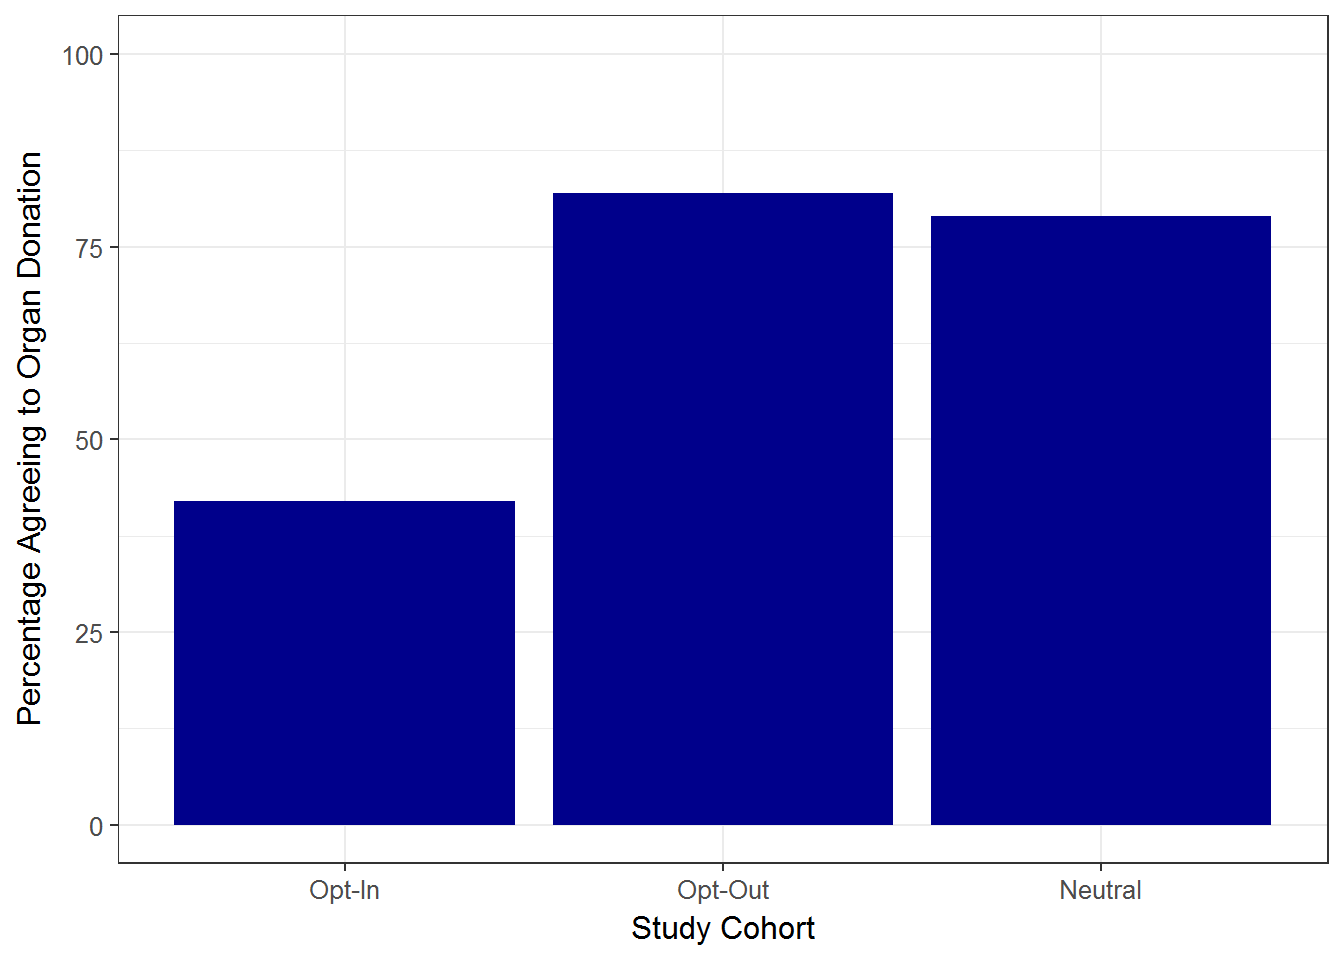
\includegraphics[width=0.8\linewidth]{./Images/basics-organ-plot-1} 

}

\caption{Summary of the responses for the Organ
Donation Study described in Example \ref{ex:basics-organ-donation}.}\label{fig:basics-organ-plot}
\end{figure}

\section{Overview of Drawing
Inference}\label{overview-of-drawing-inference}

Let's begin by taking a step back and considering the big picture of how
data is turned into information. Every research question we pose, at its
heart, is trying to characterize a \textbf{population}, the group of
subjects of ultimate interest.

\BeginKnitrBlock{definition}[Population]
\protect\hypertarget{def:defn-population}{}{\label{def:defn-population}
\iffalse (Population) \fi{} }The collection of subjects we would like to
say something about.
\EndKnitrBlock{definition}

In the Organ Donation study, the researchers would like to say something
about Americans who are of the age to consent to organ donation; in
particular, they would like to quantify how likely it is that someone
from this group agrees to organ donation. Therefore, the population is
\emph{all Americans who are of the age to consent to organ donation}.

In general, the subjects in a population need not be people; in some
studies, the population could be a collection of screws, cell phones,
sheet metal\ldots{}whatever characterizes the objects from which we
would \emph{like to} obtain measurements. We use the phrase ``like to''
because in reality it is often impossible (or impractical) to observe
the entire population. Instead, we make observations on a subset of the
population; this smaller group is known as the \textbf{sample}.

\BeginKnitrBlock{definition}[Sample]
\protect\hypertarget{def:defn-sample}{}{\label{def:defn-sample}
\iffalse (Sample) \fi{} }The collection of subjects for which we
actually obtain measurements (data).
\EndKnitrBlock{definition}

For each subject within the sample, we obtain a collection of
measurements forming our set of data. The goal of statistical modeling
is to use the sample (the group we actually observe) to say something
about the population of interest (the group we wish we had observed);
this process is known as \textbf{statistical inference}. This process is
illustrated in Figure \ref{fig:basics-statistical-process}.

\BeginKnitrBlock{definition}[Statistical Inference]
\protect\hypertarget{def:defn-inference}{}{\label{def:defn-inference}
\iffalse (Statistical Inference) \fi{} }The process of using a sample to
characterize some aspect of the underlying population.
\EndKnitrBlock{definition}

\begin{figure}

{\centering 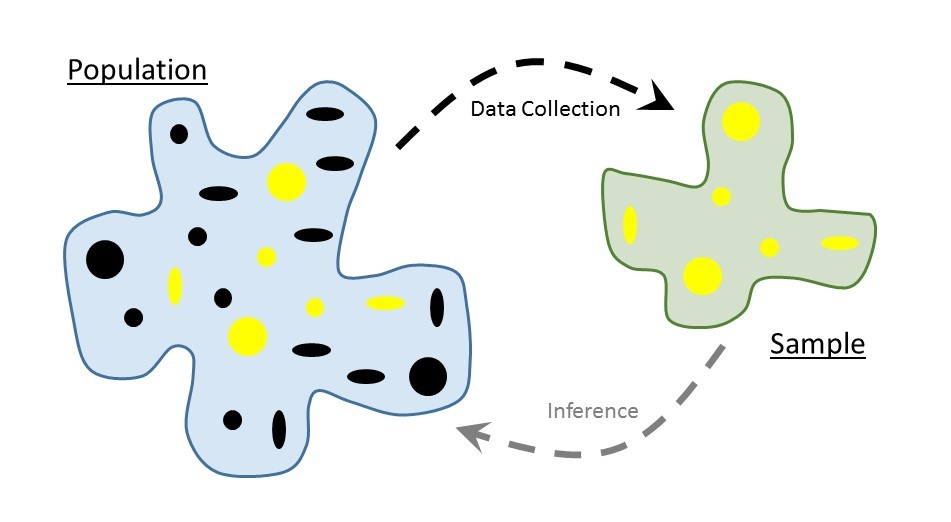
\includegraphics[width=0.8\linewidth]{images/Basics-Stat-Process} 

}

\caption{Illustration of the statistical process.}\label{fig:basics-statistical-process}
\end{figure}

\section{Anatomy of a Dataset}\label{anatomy-of-a-dataset}

Once we have our sample, we take measurements on each of the subjects
within this sample. These measurements form the data. When we hear the
word ``data,'' most of us envision a large spreadsheet. In reality, data
can take on many forms --- spreadsheets, images, text files,
unstructured text from a social media feed, etc. Regardless of the form,
all datasets contain information for each subject in the sample; this
information, the various measurements, are called \textbf{variables}.

\BeginKnitrBlock{definition}[Variable]
\protect\hypertarget{def:defn-variable}{}{\label{def:defn-variable}
\iffalse (Variable) \fi{} }A measurement, or category, describing some
aspect of the subject.
\EndKnitrBlock{definition}

Variables come in one of two flavors. \textbf{Categorical} variables are
those which denote a grouping to which the subject belongs. Examples
include marital status, brand, and experimental treatment group.
\textbf{Numeric} variables are those which take on values for which
ordinary arithmetic (e.g., addition and multiplication) makes sense.
Examples include height, age of a product, and diameter. Note that
sometimes numeric values are used to represent the levels of a
categorical variable in a dataset; for example, 0 may indicate ``No''
and 1 may indicate ``Yes'' for a variable capturing whether a person is
a registered organ donor. Therefore, just because a variable has a
numeric value does not make it a numeric variable; the key here is that
numeric variables are those for which arithmetic makes sense.

\BeginKnitrBlock{definition}[Categorical Variable]
\protect\hypertarget{def:defn-categorical}{}{\label{def:defn-categorical}
\iffalse (Categorical Variable) \fi{} }Also called a ``qualitative
variable,'' a measurement on a subject which denotes a grouping or
categorization.
\EndKnitrBlock{definition}

\BeginKnitrBlock{definition}[Numeric Variable]
\protect\hypertarget{def:defn-numeric}{}{\label{def:defn-numeric}
\iffalse (Numeric Variable) \fi{} }Also called a ``quantitative
variable,'' a measurement on a subject which takes on a numeric value
\emph{and} for which ordinary arithmetic makes sense.
\EndKnitrBlock{definition}

While it may be natural to think of a dataset as a spreadsheet, not all
spreadsheets are created equal. Here, we consider datasets which have
the following characteristics:

\begin{itemize}
\tightlist
\item
  Each column contains a unique variable.
\item
  Each record (row in the dataset) corresponds to a different
  observation of the variables.
\item
  If you have multiple datasets, they should include a column in the
  table that allows them to be linked (subject identifier).
\end{itemize}

These are characteristics of ``tidy data.'' Even unstructured data such
as images or text files must be processed, often converted to tidy data,
prior to performing a statistical analysis. The above description
eliminates a common method of storing data in engineering and scientific
disciplines --- storing each sample in a different column. To
illustrate, suppose we conduct a study comparing the lifetime (in hours)
of two brands of batteries. We measure the lifetime of five batteries of
Brand A and six of Brand B. It is common to see a dataset like that in
Table \ref{tab:basics-poor-dataset}; the problem here is that the first
record of the dataset contains information on two different
observations. We have the lifetime from a battery of Brand A in the same
row as the lifetime from a battery of Brand B. This violates the second
condition of tidy data described above.

\begin{table}

\caption{\label{tab:basics-poor-dataset}Example of a common data structure which does not represent tidy data.  Data is from a hypothetical study comparing battery lifetimes (hours).}
\centering
\begin{tabular}[t]{l|l}
\hline
Brand A & Brand B\\
\hline
8.3 & 8.4\\
\hline
5.1 & 8.6\\
\hline
3.3 & 3.8\\
\hline
5.3 & 4.1\\
\hline
5.7 & 4.5\\
\hline
 & 4.0\\
\hline
\end{tabular}
\end{table}

In order to adhere to the tidy structure, we can reformat this dataset
as illustrated in Table \ref{tab:basics-good-dataset}. Here, each record
represents a unique observation and each column is a different variable.
We have also added a unique identifier.

\begin{table}

\caption{\label{tab:basics-good-dataset}Example of a tidy dataset, a good way of storing data.  Data is from a hypothetical study comparing battery lifetimes (hours).}
\centering
\begin{tabular}[t]{r|l|r}
\hline
Battery & Brand & Lifetime\\
\hline
1 & A & 8.3\\
\hline
2 & A & 5.1\\
\hline
3 & A & 3.3\\
\hline
4 & A & 5.3\\
\hline
5 & A & 5.7\\
\hline
6 & B & 8.4\\
\hline
7 & B & 8.6\\
\hline
8 & B & 3.8\\
\hline
9 & B & 4.1\\
\hline
10 & B & 4.5\\
\hline
11 & B & 4.0\\
\hline
\end{tabular}
\end{table}

It may take some time to get used to storing data in this format, but it
makes analysis easier and avoids time spent managing the data later.

\section{A Note on Codebooks}\label{a-note-on-codebooks}

A dataset on its own is meaningless if you cannot understand what the
values represent. \emph{Before} you access a dataset, you should always
review any available \textbf{codebooks}.

\BeginKnitrBlock{definition}[Codebook]
\protect\hypertarget{def:defn-codebook}{}{\label{def:defn-codebook}
\iffalse (Codebook) \fi{} }Also called a ``data dictionary,'' these
provide complete information regarding the variables contained within a
dataset.
\EndKnitrBlock{definition}

Some codebooks are excellent, with detailed descriptions of how the
variables were collected and appropriate units. Other codebooks give
only an indication of what each variable represents. Whenever you are
working with previously collected data, reviewing a codebook is the
first step; and, you should be prepared to revisit the codebook often
throughout an analysis. When you are collecting your own dataset,
constructing a codebook is essential for others to make use of your
data.

\hypertarget{CaseDeepwater}{\chapter{Case Study: Health Effects of the
Deepwater Horizon Oil Spill}\label{CaseDeepwater}}

On the evening of April 20, 2010, the \emph{Deepwater Horizon}, an oil
drilling platform positioned off the coast of Louisiana, was engulfed in
flames as the result of an explosion. The drilling rig, leased and
operated by BP, had been tasked with drilling an oil well in water
nearly 5000 feet deep. Eleven personnel were killed in the explosion.
The following screenshot is from the initial coverage by the \emph{New
York Times}\footnote{\url{http://www.nytimes.com/2010/04/22/us/22rig.html?rref=collection\%2Ftimestopic\%2FOil\%20Spills\&action=click\&contentCollection=timestopics\&region=stream\&module=stream_unit\&version=search\&contentPlacement=1\&pgtype=collection}}:




\begin{figure}

{\centering 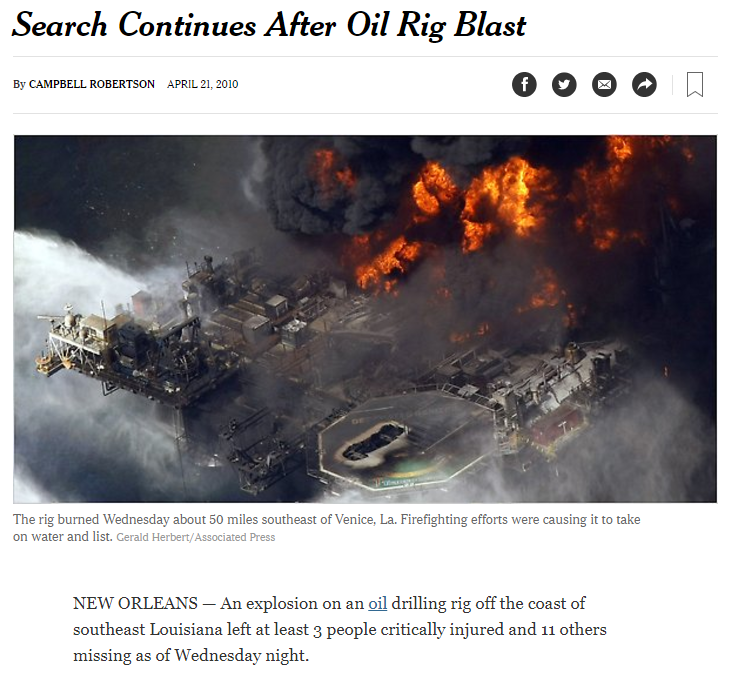
\includegraphics[width=0.8\linewidth]{./images/Case-Deepwater-NYTclip} 

}

\caption{\emph{New York Times} coverage of the
\emph{Deepwater Horizon} oil spill.}\label{fig:casedeepwater-nytclip}
\end{figure}

The incident is considered the worst oil spill in US history, creating
an environmental disaster along the Gulf Coast. In addition to studying
the effects on the local environment, researchers have undertaken
studies to examine the short and long-term health effects caused by the
incident. As an example, it is reasonable to ask whether volunteers who
were directly exposed to oil, such as when cleaning wildlife, are at
higher risk of respiratory irritation compared to those volunteers who
were helping with administrative tasks and therefore were not directly
exposed to the oil. An article appearing in \emph{The New England
Journal of Medicine} (B. D. Goldstein, Osofsky, and Lichtveld
\protect\hyperlink{ref-Goldstein2011}{2011}) reported the results from a
health symptom survey performed in the Spring and Summer of 2010 by the
National Institute for Occupational Safety and Health. Of 54 volunteers
assigned to wildlife cleaning and rehabilitation, 15 reported
experiencing ``nose irritation, sinus problems, or sore throat.'' Of 103
volunteers who had no exposure to oil, dispersants, cleaners, or other
chemicals, 16 reported experiencing ``nose irritation, sinus problems,
or sore throat.''

While a larger fraction of volunteers cleaning wildlife \emph{in the
study} reported respiratory symptoms compared to those who were not
directly exposed to irritants, would we expect similar results if we
were able to interview all volunteers? What about during a future oil
spill? Is there evidence that more than 1 in 5 volunteers who clean
wildlife will develop respiratory symptoms? What is a reasonable value
for the increased risk of respiratory symptoms for those volunteers with
direct exposure compared to those without?

In the first part of this text, we use this motivating example as the
context for discussing how research questions should be framed, methods
for data collection, summarizing and presenting data clearly,
quantifying the variability in an estimate, and quantifying the degree
to which the data disagrees with a proposed model. We capture these
ideas in what we call the \emph{Five Fundamental Ideas of Inference}. We
will also see that any statistical analysis moves between the components
of what we call the \emph{Distributional Quartet}. These two frameworks
allow us to describe the language and logic of inference, serving as a
foundation for the statistical thinking and reasoning needed to address
more complex questions encountered later in the text.

\chapter{Asking the Right Questions}\label{Questions}

The discipline of statistics is about turning data into information in
order to address some question. While there may be no such thing as a
stupid question, there are ill-posed questions --- those which cannot be
answered as stated. Consider the
\protect\hyperlink{CaseDeepwater}{Deepwater Horizon Case Study}. It
might seem natural to ask ``if a volunteer cleans wildlife, will she
develop adverse respiratory symptoms?'' Let's consider the data. Of the
54 volunteers assigned to wildlife cleaning and rehabilitation, 15
reported experiencing adverse respiratory symptoms (``nose irritation,
sinus problems, or sore throat''); while some volunteers developed
symptoms, others did not. It seems the answer to our question is then
``it depends'' or ``maybe.'' This is an example of an \emph{ill-posed
question}. Such questions exist because of \emph{variability}, the fact
that every subject in the population does not behave in exactly the same
way. In our example not every volunteer had the same reaction when
directly exposed to oil.

It is variability that creates a need for statistics; in fact, you could
think of statistics as the study and characterization of variability. We
must therefore learn to ask the \emph{right} questions --- those which
can be answered in the presence of variability.

\BeginKnitrBlock{definition}[Variability]
\protect\hypertarget{def:defn-variability}{}{\label{def:defn-variability}
\iffalse (Variability) \fi{} }The notion that measurements differ from
one observation to another.
\EndKnitrBlock{definition}

\BeginKnitrBlock{rmdkeyidea}
The presence of variability makes some questions ill-posed; statistics
concerns itself with how to address questions in the presence of
variability.
\EndKnitrBlock{rmdkeyidea}

\section{Characterizing a Variable}\label{characterizing-a-variable}

Recall that the goal of statistical inference is to say something about
the population; as a result, any question we ask should then be centered
on this larger group. The first step to constructing a well-posed
question is then to identify the population of interest for the study.
For the \protect\hyperlink{CaseDeepwater}{Deepwater Horizon Case Study},
it is unlikely that we are only interested in these 54 observed
volunteers assigned to wildlife cleaning. In reality, we probably want
to say something about volunteers for any oil spill. The 54 volunteers
in our dataset form the sample, a subset from all volunteers who clean
wildlife following an oil spill. Our population of interest is comprised
of all volunteers who clean wildlife following an oil spill.

\BeginKnitrBlock{rmdtip}
When identifying the population of interest, be specific! Suppose you
are trying to estimate the average height of trees. Are you really
interested in \emph{all} trees? Or, are you interested in Maple trees
within the city limits of Terre Haute, Indiana?
\EndKnitrBlock{rmdtip}

Since we expect that the reaction to oil exposure --- the primary
variable of interest for this study, sometimes called the
\textbf{response} --- to vary from one individual to another, we cannot
ask a question about the \emph{value} of the reaction (whether they
experienced symptoms or not). Instead, we want to characterize the
\textbf{distribution} of the response.

\BeginKnitrBlock{definition}[Response]
\protect\hypertarget{def:defn-response}{}{\label{def:defn-response}
\iffalse (Response) \fi{} }The primary variable of interest within a
study. This is the variable you would either like to explain or
estimate.
\EndKnitrBlock{definition}

\BeginKnitrBlock{definition}[Distribution]
\protect\hypertarget{def:defn-distribution}{}{\label{def:defn-distribution}
\iffalse (Distribution) \fi{} }The pattern of variability corresponding
to a set of values.
\EndKnitrBlock{definition}

Notice that in this case, the response is a categorical variable;
describing the distribution of such a variable is equivalent to
describing how individuals are divided among the possible groups. With a
finite number of observations, we could present the number of
observations (\textbf{frequeny}) within each group. For example, of the
54 volunteers, 15 experienced adverse symptoms and 39 did not. This
works well within the sample; however, as our population is infinitely
large (all volunteers cleaning wildlife following an oil spill),
reporting the frequencies is not appropriate. In this case, we report
the fraction of observations (\textbf{relative frequency}) falling
within each group; this helps convey information about the distribution
of this variable.

\BeginKnitrBlock{definition}[Frequency]
\protect\hypertarget{def:defn-frequency}{}{\label{def:defn-frequency}
\iffalse (Frequency) \fi{} }The number of observations falling into a
particular level of a categorical variable.
\EndKnitrBlock{definition}

\BeginKnitrBlock{definition}[Relative Frequency]
\protect\hypertarget{def:defn-relative-frequency}{}{\label{def:defn-relative-frequency}
\iffalse (Relative Frequency) \fi{} }Also called the ``proportion,'' the
fraction of observations falling into a particular level of a
categorical variable.
\EndKnitrBlock{definition}

Numeric quantities, like the proportion, which summarize the
distribution of a variable within the population are known as
\textbf{parameters}.

\BeginKnitrBlock{definition}[Parameter]
\protect\hypertarget{def:defn-parameter}{}{\label{def:defn-parameter}
\iffalse (Parameter) \fi{} }Numeric quantity which summarizes the
distribution of a variable within the \emph{population} of interest.
Generally denoted by Greek letters in statistical formulas.
\EndKnitrBlock{definition}

While the \emph{value} of a variable may vary across the population, the
\emph{parameter} is a single fixed constant which summarizes the
variable for that population. For example, the grade received on an exam
varies from one student to another in a class; but, the \emph{average
exam grade} is a fixed number which summarizes the class as a whole.
Well-posed questions can be constructed if we limit ourselves to
questions about the parameter. The second step in constructing
well-posed questions is then to identify the parameter of interest.

The questions we ask generally fall into one of two categories:

\begin{itemize}
\tightlist
\item
  Estimation: what \emph{proportion} of volunteers who clean wildlife
  following an oil spill will experience adverse respiratory symptoms?
\item
  Hypothesis Testing: is it reasonable to expect that no more than 1 in
  5 volunteers who clean wildlife following an oil spill will experience
  adverse respiratory symptoms?
\end{itemize}

\BeginKnitrBlock{definition}[Estimation]
\protect\hypertarget{def:defn-estimation}{}{\label{def:defn-estimation}
\iffalse (Estimation) \fi{} }Using the sample to approximate the value
of a parameter from the underlying population.
\EndKnitrBlock{definition}

\BeginKnitrBlock{definition}[Hypothesis Testing]
\protect\hypertarget{def:defn-hypothesis-testing}{}{\label{def:defn-hypothesis-testing}
\iffalse (Hypothesis Testing) \fi{} }Using a sample to determine if the
data is consistent with a working theory or if there is evidence to
suggest the data is not consistent with the theory.
\EndKnitrBlock{definition}

Since we do not get to observe the population (we only see the sample),
we cannot observe the value of the parameter. That is, we will never
know the true proportion of volunteers who experience symptoms. However,
we can determine what the data suggests about the population (that is
what inference is all about).

\BeginKnitrBlock{rmdkeyidea}
Parameters are unknown values and can, in general, never be known.
\EndKnitrBlock{rmdkeyidea}

It turns out, the vast majority of research questions can be framed in
terms of a parameter. This is the first of what we consider the
\emph{Five Fundamental Ideas of Inference}.

\BeginKnitrBlock{rmdfivefund}
\textbf{Fundamental Idea I}: A research question can often be framed in
terms of a parameter which characterizes the population. Framing the
question should then guide our analysis.
\EndKnitrBlock{rmdfivefund}

We now have a way of describing a well-posed question, a question which
can be addressed using data. Well posed questions are about the
population and can be framed in terms of a parameter which summarizes
that population. We now describe how these questions are typically
framed.

\section{Framing the Question}\label{framing-the-question}

In engineering and scientific applications, many questions fall under
the second category of model consistency. Examining such questions is
known as \textbf{hypothesis testing}, which is a form of model
comparison in which data is collected to help the researcher choose
between two competing theories for the parameter of interest. In this
section, we consider the terminology surrounding specifying such
questions.

For the \protect\hyperlink{CaseDeepwater}{Deepwater Horizon Case Study}
suppose we are interested in addressing the following question:

\begin{quote}
Is there evidence that more than 1 in 5 volunteers who clean wildlife
following an oil spill will develop adverse respiratory symptoms?
\end{quote}

The question itself is about the population (all volunteers assigned to
clean wildlife following an oil spill) and is centered on a parameter
(the proportion who develop adverse respiratory symptoms). That is, this
is a well-posed question that can be answered with appropriate data. The
overall process for addressing these types of questions is similar to
conducting a trial in a court of law. In the United States, a trial has
the following essential steps:

\begin{enumerate}
\def\labelenumi{\arabic{enumi}.}
\tightlist
\item
  Assume the defendant is innocent.
\item
  Present evidence to establish guilt, to the contrary of innocence
  (prosecution's responsibility).
\item
  Consider the weight of the evidence presented (jury's responsibility).
\item
  Make a decision. If the evidence is ``beyond a reasonable doubt,'' the
  jury declares the defendant guilty; otherwise, the jury declares the
  defendant not guilty.
\end{enumerate}

The process of conducting a hypothesis test has similar essential steps:

\begin{enumerate}
\def\labelenumi{\arabic{enumi}.}
\tightlist
\item
  Assume the opposite of what we want the data to show (develop a
  working theory).
\item
  Gather data and compare it to the proposed model from step (1).
\item
  Quantify the likelihood of our data from step (2) under the proposed
  model.
\item
  If the likelihood is small, conclude the data is not consistent with
  the working model (there is evidence for what we want to show);
  otherwise, conclude the data is consistent with the working model
  (there is no evidence for what we want to show).
\end{enumerate}

Notice that a trial focuses not on proving guilt but on disproving
innocence; similarly, in statistics, we are able to establish evidence
\emph{against} a specified theory. This is one of several subtle points
in hypothesis testing. We will discuss these subtleties at various
points throughout the text and revisit the overall concepts often. Here,
we focus solely on that first step --- developing a working theory that
we want to \emph{disprove}.

Consider the above question for the
\protect\hyperlink{CaseDeepwater}{Deepwater Horizon Case Study}. We want
to find evidence that the proportion experiencing adverse symptoms
exceeds 0.20 (1 in 5). Therefore, we would like to \emph{disprove} (or
provide evidence \emph{against}) the statement that the proportion
experiencing adverse symptoms is no more than 0.20. This is known as the
\textbf{null hypothesis}; the opposite of this statement, called the
\textbf{alternative hypothesis}, captures what we would like to
establish.

\BeginKnitrBlock{definition}[Null Hypothesis]
\protect\hypertarget{def:defn-null-hypothesis}{}{\label{def:defn-null-hypothesis}
\iffalse (Null Hypothesis) \fi{} }The statement (or theory) that we
would like to \emph{disprove}. This is denoted \(H_0\), read
``H-naught'' or ``H-zero''.
\EndKnitrBlock{definition}

\BeginKnitrBlock{definition}[Alternative Hypothesis]
\protect\hypertarget{def:defn-alternative-hypothesis}{}{\label{def:defn-alternative-hypothesis}
\iffalse (Alternative Hypothesis) \fi{} }The statement (or theory)
capturing what we would like to provide evidence \emph{for}; this is the
opposite of the null hypothesis. This is denoted \(H_1\) or \(H_a\),
read ``H-one'' and ``H-A'' respectively.
\EndKnitrBlock{definition}

For the \protect\hyperlink{CaseDeepwater}{Deepwater Horizon Case Study},
we write:

\begin{quote}
\(H_0:\) The proportion of volunteers assigned to clean wildlife
following an oil spill who experience adverse respiratory symptoms is no
more than 0.20.\\
\(H_1:\) The proportion of volunteers assigned to clean wildlife
following an oil spill who experience adverse respiratory symptoms
exceeds 0.20.
\end{quote}

Each hypothesis is a well-posed statement (about a parameter
characterizing the entire population), and the two statements are
exactly opposite of one another meaning only one can be a true
statement.

\BeginKnitrBlock{rmdtip}
When framing your questions, be sure your null hypothesis and
alternative hypothesis are exact opposites of one another, and ensure
the ``equality'' component \emph{always} goes in the null hypothesis.
\EndKnitrBlock{rmdtip}

We can now collect data and determine if it is consistent with the null
hypothesis (a statement similar to ``not guilty'') or if the data
provides evidence against the null hypothesis and in favor of the
alternative (a statement similar to ``guilty'').

Often these statements are written in a bit more of a mathematical
structure in which a Greek letter is used to represent the parameter of
interest. For example, we might write

\begin{quote}
Let \(\theta\) be the proportion of volunteers (assigned to clean
wildlife following an oil spill) who experience adverse respiratory
symptoms.\\
\(H_0: \theta \leq 0.20\)\\
\(H_1: \theta > 0.20\)
\end{quote}

In the above statements, \(\theta\) represents the parameter of
interest; the value 0.20 is known as the \textbf{null value}.

\BeginKnitrBlock{definition}[Null Value]
\protect\hypertarget{def:defn-null-value}{}{\label{def:defn-null-value}
\iffalse (Null Value) \fi{} }The value associated with the equality
component of the null hypothesis; it forms the threshold or boundary
between the two hypothesis. Note: not all questions of interest require
a null value be specified.
\EndKnitrBlock{definition}

\BeginKnitrBlock{rmdkeyidea}
Hypothesis testing is a form of statistical inference in which we
quantify the evidence \emph{against} a working theory (captured by the
null hypothesis). We essentially argue that the data supports the
alternative if it is not consistent with the working theory.
\EndKnitrBlock{rmdkeyidea}

This section has focused on developing the null and alternative
hypothesis when our question of interest is best characterized as one of
comparing models or evaluating a particular statement. If our goal is
estimation, a null and alternative hypothesis are not applicable. For
example, we might have the following goal:

\begin{quote}
Estimate the proportion of volunteers (assigned to clean wildlife
following an oil spill) who experience adverse respiratory symptoms.
\end{quote}

In this version of our research ``question'' there is no statement which
needs to be evaluated. We are interested in estimation, not hypothesis
testing and thus there is no corresponding null and alternative
hypothesis.

\BeginKnitrBlock{rmdtip}
\textbf{Process for Framing a Question} In order to frame a research
question, consider the following steps:

\begin{enumerate}
\def\labelenumi{\arabic{enumi}.}
\tightlist
\item
  Identify the population of interest.
\item
  Identify the parameter(s) of interest.
\item
  Determine if you are interested in estimating the parameter(s) or
  quantifying the evidence against some working theory.
\item
  If you are interested in testing a working theory, make the null
  hypothesis the working theory and the alternative the exact opposite
  statement (what you want to provide evidence for).
\end{enumerate}
\EndKnitrBlock{rmdtip}

\chapter{Gathering the Evidence (Data Collection)}\label{Data}

Consider again the goal of statistical inference --- to use a sample as
a snapshot to say something about the underlying population (Figure
\ref{fig:data-statistical-process}). This generally provokes unease in
people, leading to a distrust of statistical results. In this section we
attack that distrust head on.

\begin{figure}

{\centering 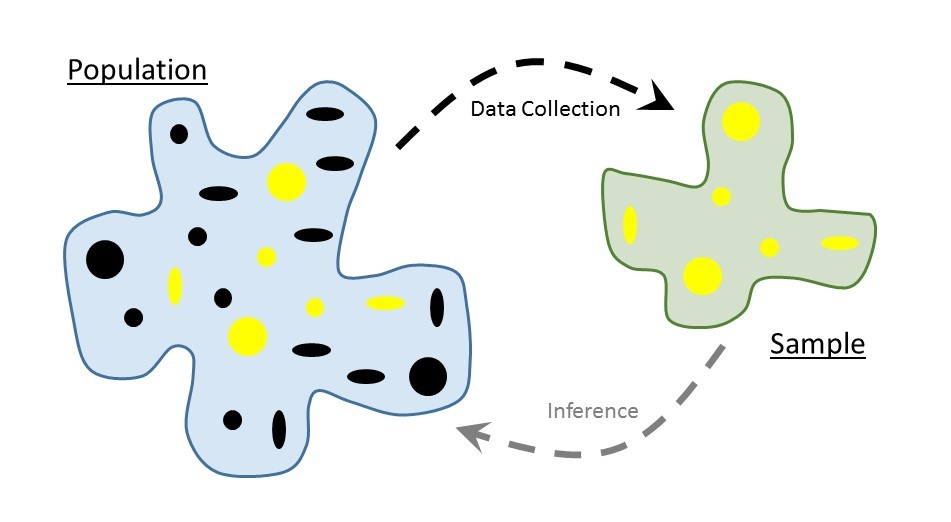
\includegraphics[width=0.8\linewidth]{images/Basics-Stat-Process} 

}

\caption{Illustration of the statistical process (reprinted from Chapter 1).}\label{fig:data-statistical-process}
\end{figure}

\section{What Makes a Sample
Reliable}\label{what-makes-a-sample-reliable}

If we are going to have some amount of faith in the statistical results
we produce, we must have data in which we can place our trust. \emph{The
Treachery of Images} (Figure \ref{fig:data-pipe-img}) is a canvas
painting depicting a pipe, below which the artist wrote the French
phrase ``This is not a pipe.'' Regarding the painting, the artist said

\begin{quote}
The famous pipe. How people reproached me for it! And yet, could you
stuff my pipe? No, it's just a representation, is it not? So if I had
written on my picture ``This is a pipe,'' I'd have been lying!
\end{quote}




\begin{figure}

{\centering 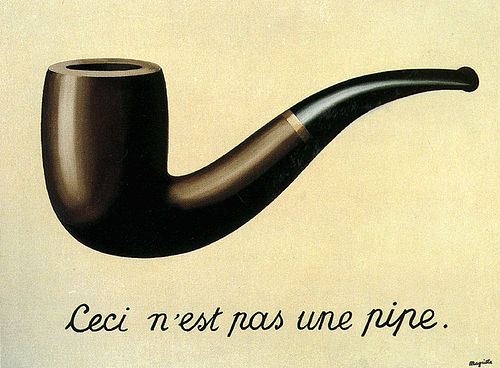
\includegraphics[width=0.8\linewidth]{./images/Data-Pipe} 

}

\caption{\emph{The Treachery of Images} by René
Magritte.}\label{fig:data-pipe-img}
\end{figure}

Just as a painting is a representation of the object it depicts, so a
sample should be a representation of the population under study. This is
the primary requirement if we are to rely on the resulting data.

\BeginKnitrBlock{rmdkeyidea}
In order for a statistical analysis to be reliable, the sample must be
\emph{representative} of the population under study.
\EndKnitrBlock{rmdkeyidea}

We need to be careful to not get carried away in our expectations. What
constitutes ``representative'' really depends on the question, just as
an artist chooses his depiction based on how he wants to represent the
object. Let's consider the following example.

\BeginKnitrBlock{example}[School Debt]
\protect\hypertarget{exm:data-school-debt}{}{\label{exm:data-school-debt}
\iffalse (School Debt) \fi{} }In addition to a degree, college graduates
also tend to leave with a large amount of debt due to college loans. In
2012, a graduate with a student loan had an average debt of \$29,400;
for graduates from private non-profit institutions, the average debt was
\$32,300\footnote{\url{http://ticas.org/sites/default/files/pub_files/Debt_Facts_and_Sources.pdf}}.

Suppose we are interested in determining the average amount of debt in
student loans carried by a graduating senior from Rose-Hulman Institute
of Technology, a small private non-profit engineering school. There are
many faculty at Rose-Hulman who choose to send their children to the
institute. Since I am also on the faculty, I know many of these
individuals. Suppose I were to ask each to report the amount of student
loans their children carried upon graduation from Rose-Hulman. I compile
the 25 responses and compute the average amount of debt. Further, I
report that based on this study, there is significant evidence that the
average debt carried by a graduate of Rose-Hulman is far below the
\$32,300 reported above (great news for this year's graduating class)!
Why might we be hesitant to trust these results?
\EndKnitrBlock{example}

Many objections to statistical results stem from a distrust of whether
the data (the sample) is really representative of the population of
interest. Rose-Hulman, like many other universities, has a policy that
the children of faculty may attend their university (assuming
admittance) tuition-free. We would therefore expect their children to
carry much less debt than the typical graduating senior. There is a
mismatch between the group we would like to study and the data we have
collected.

This example provides a nice backdrop for discussing what it means to be
representative. First, let's define our population; in this case, we are
interested in graduating seniors from Rose-Hulman. The variable of
interest is the amount of debt carried in student loans; the parameter
of interest is then the \emph{average} amount of debt in student loans
carried by graduating seniors of Rose-Hulman. However, the sample
consists of only graduating seniors of Rose-Hulman who have a parent
employeed by the university.

With regard to the grade point average of the students in our sample, it
is probably similar to all graduating seniors. The starting salary of
the students in our sample is probably similar to all graduating
seniors; the fraction of mechanical engineering majors versus math
majors is probably similar. So, in many regards the sample is
representative of the population; however, it fails to be representative
with regard to the variable of interest. This is our concern. The amount
of debt carried by students in our sample is not representative of that
debt carried by all graduating seniors from the university.

\BeginKnitrBlock{rmdtip}
When thinking about whether a sample is representative, focus your
attention to the characteristics specific to your research question.
\EndKnitrBlock{rmdtip}

Does that mean the sample is useless? Yes and no. The sample collected
cannot be used to answer our initial question of interest. No
statistical method can fix bad data; statistics adheres to the
``garbage-in, garbage-out'' phenomena. If the data is bad, no analysis
will undo that. However, while the sample cannot be used to answer our
initial question, it could be used to address a different question:

\begin{quote}
What is the average amount of debt in student loans carried by
graduating seniors from Rose-Hulman whose parent is a faculty member at
the university?
\end{quote}

For this revised question, the sample may indeed be representative. If
we are working with previously collected data, we must consider the
population to which our results will generalize. That is, for what
population is the given sample representative? If we are collecting our
data, we need to be sure we collect data in such a way that the data is
representative of our target population. Let's first look at what
\emph{not} to do.

\section{Poor Methods of Data
Collection}\label{poor-methods-of-data-collection}

Example \ref{ex:data-school-debt} is an example of a ``convenience
sample,'' when the subjects in the sample are chosen simply due to ease
of collection. Examples include surveying students only in your sorority
when you are interested in all females who are part of a sorority on
campus; taking soil samples from only your city when you are interested
in the soil for the entire state; and, obtaining measurements from only
one brand of phone, because it was the only one you could afford on your
budget, when you are interested in studying all cell phones on the
market. A convenience sample is unlikely to be representative if there
is a relationship between the ease of collection and the variable under
study. This was true in the School Debt example; the relationship of a
student to a faculty member was directly related to the amount of debt
they carried. As a result, the resulting sample was not representative
of the population.

When conducting a survey with human subjects, it is common to only
illicit responses from volunteers. Such ``volunteer samples'' tend to
draw in those with extreme opinions. Consider product ratings on Amazon.
Individual ratings tend to cluster around 5's and 1's. This is because
those customers who take time to submit a review (which is voluntary)
tend to be those who are really thrilled with their product (and want to
encourage others to purchase it) and those who are really disappointed
with their purchase (and want to encourage others to avoid it). Such
surveys often fail to capture those individuals in the population who
have ``middle of the road'' opinions.

We could not possibly name all the poor methods for collecting a sample;
but, poor methods all share something in common --- it is much more
likely the resulting sample is not representative. Failing to be
representative results in \textbf{biased} estimates of the parameter.

\BeginKnitrBlock{definition}[Bias]
\protect\hypertarget{def:defn-bias}{}{\label{def:defn-bias} \iffalse (Bias)
\fi{} }A set of measurements is said to be biased if they are
\emph{consistently} too high (or too low). Similarly, an estimate of a
parameter is said to be biased if it is \emph{consistently} too high (or
too low).
\EndKnitrBlock{definition}

To illustrate the concept of bias, consider shooting at a target as in
Figure \ref{fig:data-bias}. We can consider the center of our target to
be the parameter we would like to estimate within the population. The
values in our sample (the strikes on the target) will vary around the
parameter; while we do not expect any one value to hit the target
precisely, a ``representative'' sample is one in which the values tend
to be clustered about the parameter (unbiased). When the sample is not
representative, the values in the sample tend to cluster off the mark
(biased). Notice that to be unbiased, it may be that not a single value
in the sample is perfect, but aggregated together, they point in the
right direction. So, bias is not about an individual measurement being
an ``outlier,'' (more on those in a later chapter) but about repeatedly
shooting in the wrong direction.

\begin{figure}

{\centering 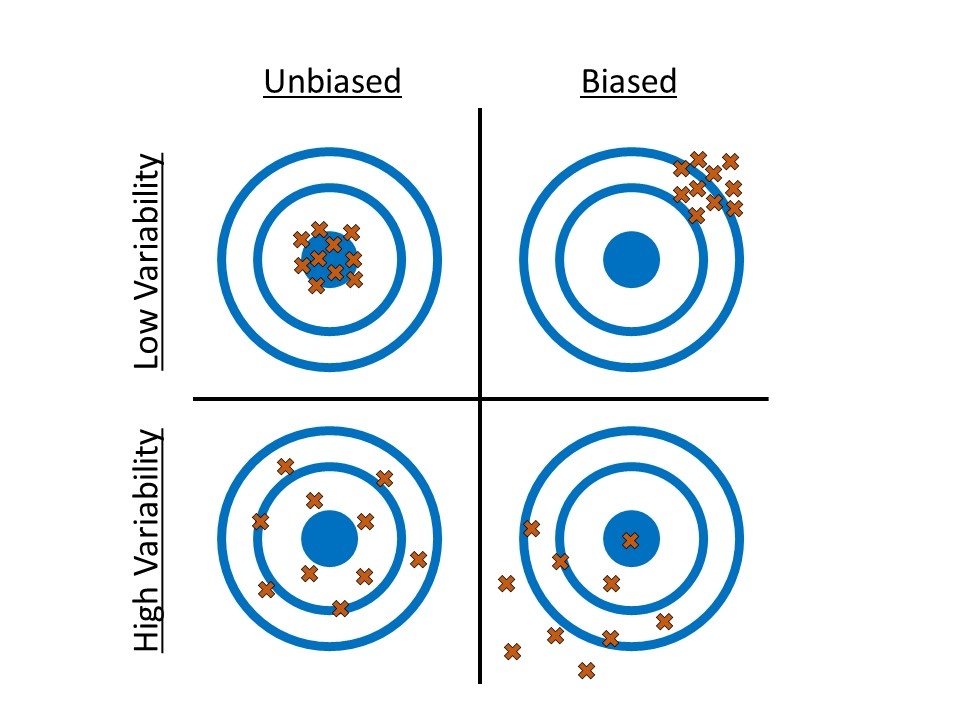
\includegraphics[width=0.8\linewidth]{./images/Data-Bias} 

}

\caption{Illustration of bias and variability.}\label{fig:data-bias}
\end{figure}

\BeginKnitrBlock{rmdkeyidea}
Biased results are typically due to poor sampling methods that result in
a sample which is not representative of the target population.
\EndKnitrBlock{rmdkeyidea}

The catch (there is always a catch) is that we will never \emph{know} if
a sample is actually representative or not. We can, however, employ
methods that help to minimize the chance that the sample is biased.

\section{Preferred Methods of
Sampling}\label{preferred-methods-of-sampling}

No method guarantees a perfectly representative sample; but, we can take
measures to reduce or eliminate bias. A useful strategy is to employ
\emph{randomization}. This is summarized in our second Fundamental Idea:

\BeginKnitrBlock{rmdfivefund}
\textbf{Fundamental Idea II}: If data is to be useful for making
conclusions about the population, a process referred to as drawing
inference, proper data collection is crucial. Randomization can play an
important role ensuring a sample is representative and that inferential
conclusions are appropriate.
\EndKnitrBlock{rmdfivefund}

Consider the School Debt example again. Suppose instead of the strategy
described there, we had done the following:

\begin{quote}
We constructed a list of all graduating seniors from the university. We
placed the name of each student on an index card; then, we thoroughly
shuffled the cards and chose the top 25 cards. For these 25 individuals,
we recorded the amount of debt in student loans each carried.
\end{quote}

This essentially describes using a lottery to select the sample. This
popular method is known as taking a \textbf{simple random sample}. By
conducting a lottery, we make it very unlikely that our sample consists
of only students with a very small amount of student debt (as occurred
when we used a convenience sample).

\BeginKnitrBlock{definition}[Simple Random Sample]
\protect\hypertarget{def:defn-simple-random-sample}{}{\label{def:defn-simple-random-sample}
\iffalse (Simple Random Sample) \fi{} }Often abbreviated SRS, this is a
sample of size \(n\) such that \emph{every} collection of size \(n\) is
equally likely to be the resulting sample. This is equivalent to a
lottery.
\EndKnitrBlock{definition}

There are situations in which a simple random sample does not suffice.
Again, consider our School Debt example. The Rose-Hulman student body is
predominantly domestic, with only about 3\% of the student body being
international students. But, suppose we are interested in comparing the
average debt carried between international and domestic students. It is
very likely, by chance alone, that in a simple random sample of 25
students none will be international. Instead of a simple random sample,
we might consider taking a sample of 13 domestic students and a sample
of 12 international students; this is an example of a \textbf{stratified
random sample}. This approach is useful when there is a natural grouping
of interest within the population.

\BeginKnitrBlock{definition}[Stratified Random Sample]
\protect\hypertarget{def:defn-stratified-random-sample}{}{\label{def:defn-stratified-random-sample}
\iffalse (Stratified Random Sample) \fi{} }A sample in which the
population is first divided into groups, or strata, based on a
characteristic of interest; a simple random sample is then taken within
each group.
\EndKnitrBlock{definition}

There are countless sampling techniques used in practice. The two
described above can be very useful starting points for developing a
custom method suitable for a particular application. Their benefit stems
from their use of randomization.

This section is entitled ``Preferred Methods'' because while these
methods are ideal, they are not always practical. Consider the
\protect\hyperlink{CaseDeepwater}{Deepwater Horizon Case Study};
conceptually, we can take a simple random sample of the volunteers for
our study. However, as with any study involving human subjects,
researchers would be required to obtain consent from each subject in the
study. That is, a volunteer has the right to refuse to participate in
the study. Therefore, it is unlikely that a simple random sample as
described above could be obtained. Again, the key is to obtain a
\emph{representative} sample; while random selection may be a nice tool
for accomplishing this, we may need to appeal to the composition of the
sample itself to justify its use. \emph{Based on the characteristics of
those willing to participate in the study, do we feel the study
participants form a representative group of all volunteers?} That is the
essential question. This is often why studies report a table summarizing
subject demographics such as age, gender, etc. It is also why it is
extremely important for researchers to describe how subjects were
selected so that readers may make the judgement for themselves whether
the sample is representative.

\section{Two Types of Studies}\label{two-types-of-studies}

Thinking about how the data was collected helps us determine how the
results generalize beyond the sample itself (to what population the
results apply). When our question of interest is about the relationship
between two variables (as most questions are), we must also carefully
consider the study design. Too often separated from the statistical
analysis that follows, keeping the study design in mind should guide the
analysis as well as inform us about the conclusions we can draw.

In order to illustrate how study design can impact the results, consider
the following example.

\BeginKnitrBlock{example}[Kangaroo Care]
\protect\hypertarget{exm:data-kangaroo}{}{\label{exm:data-kangaroo}
\iffalse (Kangaroo Care) \fi{} }At birth, infants have low levels of
Vitamin K, a vitamin needed in order to form blood clots. Though rare,
without the ability for her blood to clot, an infant could develop a
serious bleed. In order to prevent this, the American Academy of
Pediatrics recommends that all infants be given a Vitamin K shot shortly
after birth in order to raise Vitamin K levels. As with any shot, there
is typically discomfort to the infant, which can be very discomforting
to new parents.

Kangaroo Care is a method of holding a baby which emphasizes
skin-to-skin contact. The child, who is dressed only in a diaper, is
placed upright on the parent's bare chest; a light blanket is draped
over the child. Suppose we are interested in determining if utilizing
the method while giving the child a Vitamin K shot reduces the
discomfort in the infant, as measured by the total amount of time the
child cries following the shot. Contrast the following two potential
study designs:

\begin{enumerate}
\def\labelenumi{(\Alph{enumi})}
\tightlist
\item
  We allow the attending nurse to determine whether Kangaroo Care is
  initiated prior to giving the Vitamin K shot. Following the shot, we
  record the total time (in seconds) the child cries.
\item
  We flip a coin. If it comes up heads, the nurse should have the
  parents implement Kangaroo Care prior to giving the Vitamin K shot; if
  it comes up tails, the nurse should give the Vitamin K shot without
  implementing Kagaroo Care. Following the shot, we record the total
  time (in seconds) the child cries.
\end{enumerate}

Note, in both study designs (A) and (B), we only consider term births
which have no complications to avoid situations that might alter the
timing of the Vitamin K shot or the ability to implement Kangaroo Care.
\EndKnitrBlock{example}

Note that there are some similarities in the two study designs:

\begin{itemize}
\tightlist
\item
  The underlying population is the same for both designs --- infants
  born at term with no complications.
\item
  There are two groups being compared in both designs --- the ``Kangaroo
  Care'' group and the ``no Kangaroo Care'' group.
\item
  The response (variable of interest) is the same in both designs ---
  the time (in seconds) the infant cries.
\item
  There is action taken by the researcher in both designs --- a Vitamin
  K shot is given to the child.
\end{itemize}

There is one prominent difference between the two study designs:

\begin{itemize}
\tightlist
\item
  For design (A), the choice of Kangaroo Care is left up to the nurse
  (self-selected); for design (B), the choice of Kangaroo is
  \emph{assigned} to the nurse by the researcher, and this selection is
  made \emph{at random}.
\end{itemize}

Design (A) is an example of an \textbf{observational study}; design (B)
is a \textbf{controlled experiment}.

\BeginKnitrBlock{definition}[Observational Study]
\protect\hypertarget{def:defn-observational-study}{}{\label{def:defn-observational-study}
\iffalse (Observational Study) \fi{} }A study in which each subject
``self-selects'' into one of groups being compared in the study. The
phrase ``self-selects'' is used very loosely here and can include
studies in which the groups are defined by an inherit characteristic or
the groups are chosen haphazardly.
\EndKnitrBlock{definition}

\BeginKnitrBlock{definition}[Controlled Experiment]
\protect\hypertarget{def:defn-controlled-experiment}{}{\label{def:defn-controlled-experiment}
\iffalse (Controlled Experiment) \fi{} }A study in which each subject is
\emph{randomly} assigned to one of the groups being compared in the
study.
\EndKnitrBlock{definition}

It is common to think that anytime the environment is ``controlled'' by
the researcher that a controlled experiment is taking place, but the
defining characteristic is the random assignment to groups (sometimes
referred to as the \emph{factor} under study or \emph{treatment}
groups). In the example above, both study designs involved a controlled
setting (the delivery room of a hospital) in which trained staff (the
nurse) deliver the shot. However, only design (B) is a controlled
experiment because the researchers randomly determined into which group
the infant would be placed.

To understand the impact of random allocation, suppose that we had
conducted a study using design (A); further, the results suggest that
those infants who were given a shot while using Kangaroo Care cried for
a shorter time period, on average. Can we conclude that it was the
Kangaroo Care that led to the shorter crying time? Maybe. Consider the
following two potential explanations for the resulting data:

\begin{enumerate}
\def\labelenumi{(\arabic{enumi})}
\tightlist
\item
  Kangaroo Care is very effective; as a result, those children who were
  given Kangaroo Care had reduced crying time, on average, following the
  Vitamin K shot.
\item
  It turns out that those nurses who chose to implement Kangaroo Care
  (remember, they have a choice under design (A) whether they implement
  the method) were also the nurses with a gentler bedside manner.
  Therefore, these nurses tended to be very gentle when giving the
  Vitamin K shot whereas the nurses who chose not to implement Kangaroo
  Care tended to just jab the needle in when giving the shot. As a
  result, the reduced crying time is not a result of the Kangaroo Care
  but the manner in which the shot was given.
\end{enumerate}

The problem is that we are unable to determine which of the explanations
is correct. Given the data we have collected, we are unable to tease out
the effect of the Kangaroo Care from that of the nurse's bedside manner.
As a result, we are able to say we observed an \emph{association}
between the use of Kangaroo Care and reduced crying time, but we are
unable to conclude that Kangaroo Care \emph{caused} a reduction in the
crying time (that is, there may not be a \emph{relationship} between the
two variables). In this hypothetical scenario, the nurse's bedside
manner is called a \textbf{confounder}.

\BeginKnitrBlock{definition}[Confounding]
\protect\hypertarget{def:defn-confounding}{}{\label{def:defn-confounding}
\iffalse (Confounding) \fi{} }When the effect of a variable on the
response is mis-represented due to the presence of a third, potentially
unobserved, variable known as a confounder.
\EndKnitrBlock{definition}

Confounders can mask the relationship between the factor under study and
the response. There is a documented association between ice cream sales
and the risk of shark attacks. As ice cream sales increase, the risk of
a shark attack also tends to increase. This does not mean that if a
small city in the Midwest increases its ice cream sales that the
citizens are at higher risk of being attacked by a shark. As Figure
\ref{fig:data-confounding} illustrates, there is a confounder ---
temperature. As the temperatures increase, people tend to buy more ice
cream; as the temperature increases, people tend to go to the beach
increasing the risk of a shark attack. Two variables can appear to be
related as a result of a confounder.

\begin{figure}

{\centering 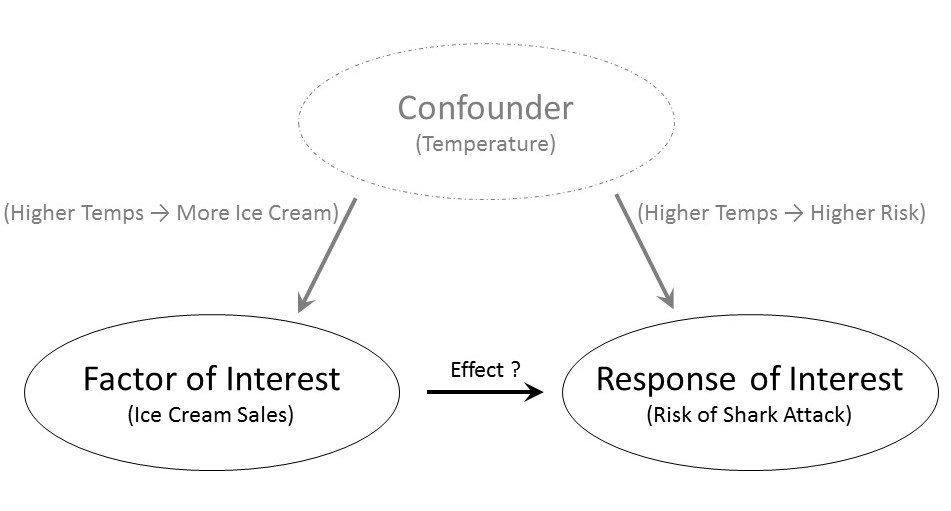
\includegraphics[width=0.8\linewidth]{./images/Data-Confounding} 

}

\caption{Illustration of a confounding variable. The confounder, related to both the factor and the treatment can make it appear as though there is a causal relationship when none exists.}\label{fig:data-confounding}
\end{figure}

\BeginKnitrBlock{rmdtip}
Confounders are variables that influence \emph{both} the factor of
interest and the response.
\EndKnitrBlock{rmdtip}

Observational studies are subject to confounding; thus, controlled
experiments are often considered the gold standard in research because
they allow us to infer cause-and-effect relationships from the data. Why
does the random allocation make such an impact? Because it removes the
impact of confounders. Let's return to the hypothetical Vitamin-K study.
Suppose there are nurses with a gentle bedside manner and those who are
a little less gentle. If the infants are randomly assigned to one of the
two treatment groups, then for every gentle nurse who is told to
implement Kangaroo Care while giving the shot, there tends to be a
gentle nurse who is told to not implement Kangaroo Care. Similarly, for
every mean nurse who is told to implement Kangaroo Care while giving a
shot, there tends to be a mean nurse who is told to not implement
Kangaroo Care. This is illustrated in Figure
\ref{fig:data-randomization}. For an observational study, the treatment
groups can be unbalanced; for example, the figure illustrates a case in
which there is a higher fraction (11/12 compared to 1/4) of friendly
nurses in the Kangaroo Care group compared to the No Kangaroo Care
group. For the controlled experiment however, the treatment groups tend
to be balanced; there is approximately the same fraction of friendly
nurses in both groups. Random assignment is the great equalizer. It
tends to result in groups which are similar in all respects; therefore,
any differences we observe between the groups \emph{must} be due to the
grouping and not an underlying confounding variable.

\begin{figure}

{\centering 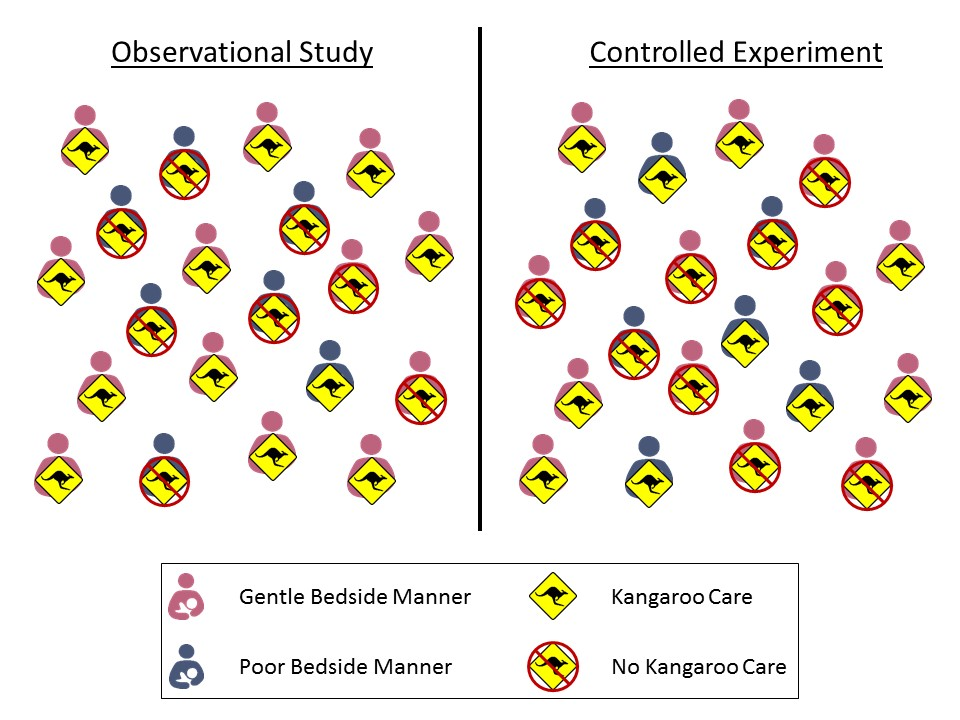
\includegraphics[width=0.8\linewidth]{./images/Data-Randomization} 

}

\caption{Illustration of the impact of random assignment in study design. For the observational study, the treatment groups are unbalanced.  For the controlled experiment, the treatment groups are balanced.}\label{fig:data-randomization}
\end{figure}

\BeginKnitrBlock{rmdkeyidea}
Randomly assigning subjects to groups balances the groups with respect
to any confounders; that is, the groups being compared are similar.
Therefore, any differences between the two groups can be attributed to
the grouping factor itself, leading to cause-and-effect conclusions.
\EndKnitrBlock{rmdkeyidea}

While controlled experiments are a fantastic study design, we should not
discount the use of observational studies. Consider the
\protect\hyperlink{CaseDeepwater}{Deepwater Horizon Case Study}; suppose
we are interested in the following question:

\begin{quote}
Is there evidence that volunteers who are directly exposed to oil have
an increased risk of developing adverse respiratory symptoms compared to
those who are not directly exposed to oil?
\end{quote}

The response is whether a volunteer develops adverse respiratory
symptoms; the factor of interest is whether the volunteer has direct
exposure to oil. We could conduct a controlled experiment by randomly
determining which volunteers are assigned to wildlife clean up and which
are assigned to administrative tasks, for example. However, it may be
that volunteer tasks need to be determined by skillset or by greatest
need at the time the person volunteers. It may not be feasible to
randomly assign volunteers to specific positions. Or, it could be that
the data was obtained after the fact; that is, the data is not the
result of a planned study in which case random assignment is not
possible because volunteers self-selected into positions in the past. If
random assignment is not possible, it does not mean the data is useless.
But, it does mean we will need to be sure we address the potential
confounding when performing the analysis and discussing the results.

The big idea is that in order to make causal conclusions, we must be
able to state that the groups being compared are balanced with respect
to any potential confounders; random assignment is one technique for
accomplishing this.

\chapter{Presenting the Evidence (Summarizing Data)}\label{Summaries}

If you open any search engine and look up ``data visualization,'' you
will quickly be overwhelmed by a host of pages, texts, and software
filled with tools for summarizing your data. Here is the bottom line: a
good visualization is one that helps you answer your question of
interest. It is both that simple and that complicated.

\BeginKnitrBlock{rmdfivefund}
\textbf{Fundamental Idea III}: The use of data for decision making
requires that the data be summarized and presented in ways that address
the question of interest.
\EndKnitrBlock{rmdfivefund}

Whether simple or complex, all graphical and numerical summaries should
help turn the data into usable information. Pretty pictures for the sake
of pretty pictures are not helpful. In this section, we will consider
various simple graphical and numerical summaries to help build a case
for addressing the question of interest.

\section{Characteristics of a Distribution (Summarizing a Single
Variable)}\label{characteristics-of-a-distribution-summarizing-a-single-variable}

Remember that because of \emph{variability}, the key to asking good
questions is to not ask questions about individual values but to
characterize the underlying \emph{distribution} (see Definition
\ref{def:defn-distribution}). Therefore, characterizing the underlying
distribution is also the key to a good visualization or numeric summary.
For the \protect\hyperlink{CaseDeepwater}{Deepwater Horizon Case Study},
the response (whether a volunteer experienced adverse respiratory
symptoms) is categorical. As we stated previously, summarizing the
distribution of a categorical variable reduces to showing how individual
subjects fall into the various groups. Figure
\ref{fig:summaries-deepwater-barchart} displays a \emph{bar chart}
summarizing the rate of respiratory symptoms for volunteers cleaning
wildlife.

\begin{figure}

{\centering 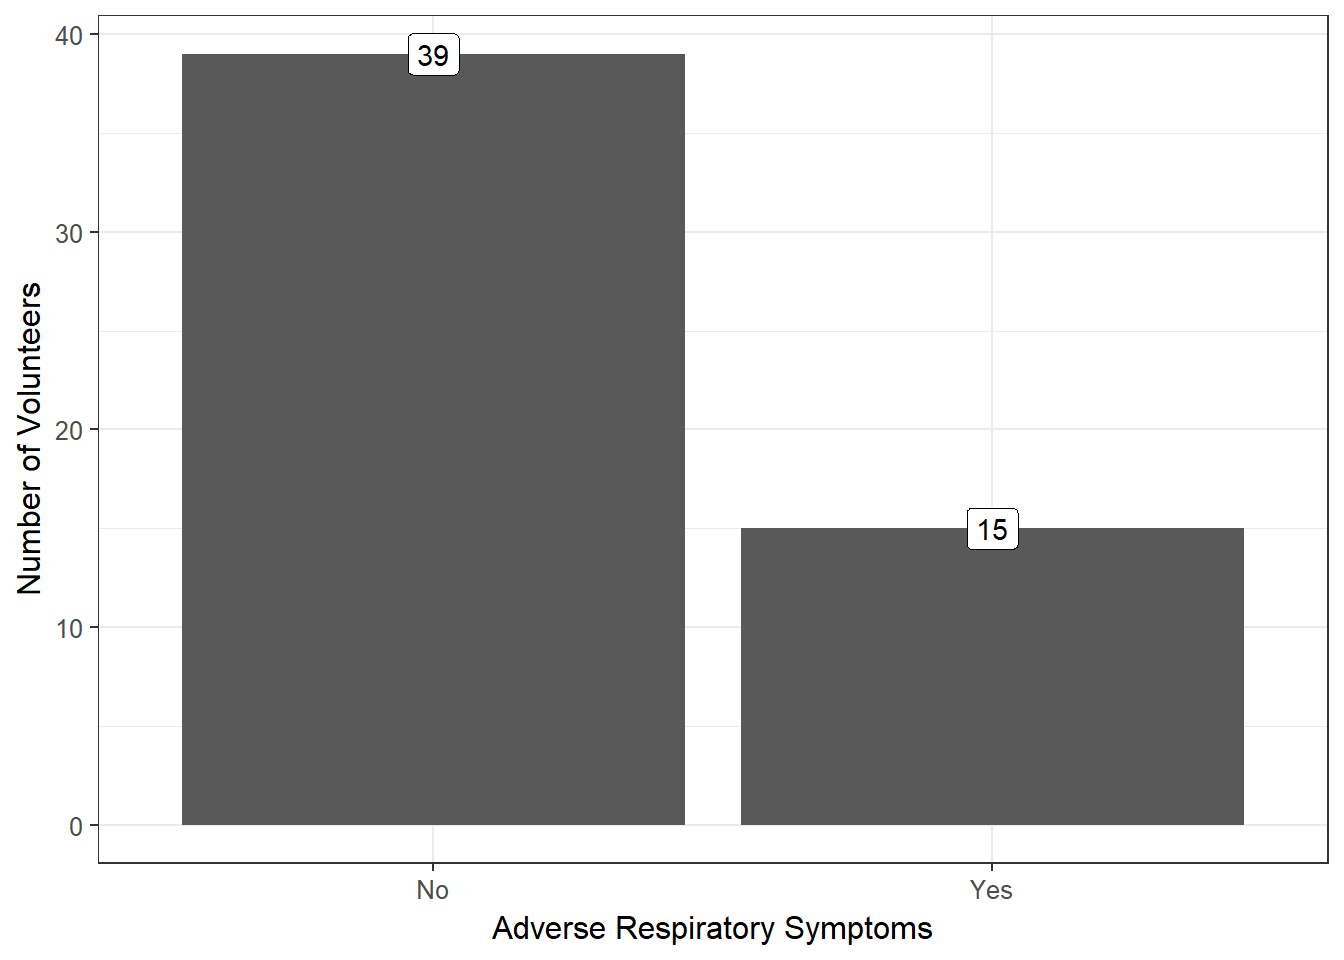
\includegraphics[width=0.8\linewidth]{./Images/summaries-deepwater-barchart-1} 

}

\caption{Frequency of adverse respiratory symptoms for volunteers cleaning wildlife following the Deepwater Horizon oil spill.}\label{fig:summaries-deepwater-barchart}
\end{figure}

In general, it does not matter whether the frequency or the relative
frequencies are reported; however, if the relative frequencies are
plotted, some indication of the sample size should be provided with the
figure either as an annotation or within the caption. From the above
graphic, we see that nearly 28\% of volunteers assigned to wildlife
experienced adverse respiratory symptoms; the graphic helps address our
question, even if not definitively.

\BeginKnitrBlock{rmdtip}
When you are summarizing only categorical variables, a bar chart is
sufficient. Statisticians tend to agree that bar charts are preferable
to pie charts (see
\href{https://www.google.com/url?sa=t\&rct=j\&q=\&esrc=s\&source=web\&cd=32\&cad=rja\&uact=8\&ved=0ahUKEwjk6Lf42sfVAhVl64MKHaTdAFY4HhAWCC4wAQ\&url=https\%3A\%2F\%2Fwww.perceptualedge.com\%2Farticles\%2Fvisual_business_intelligence\%2Fsave_the_pies_for_dessert.pdf\&usg=AFQjCNFkS-sogmLsZIOheWAPBZSNcqjzkg}{this
whitepaper} and
\href{http://www.storytellingwithdata.com/blog/2014/06/alternatives-to-pies}{this
blog} for further explanation).
\EndKnitrBlock{rmdtip}

While a single type of graphic (bar charts) are helpful for looking at
categorical data, summarizing the distribution of a numeric variable
requires a bit more thought. Consider the following example.

\BeginKnitrBlock{example}[Paper Strength]
\protect\hypertarget{exm:summaries-paper}{}{\label{exm:summaries-paper}
\iffalse (Paper Strength) \fi{} }While electronic records have become
the predominant means of storing information, we do not yet live in a
paperless society. Paper products are still used in a variety of
applications ranging from printing reports and photography to packaging
and bathroom tissue. In manufacturing paper for a particular
application, the strength of the resulting paper product is a key
characteristic.

There are several metrics for the strength of paper. A conventional
metric for assessing the inherent (not dependent upon the physical
characteristics, such as the weight of the paper, which might have an
effect) strength of paper is the \emph{breaking length}. This is the
length of a paper strip, if suspended vertically from one end, that
would break under its own weight. Typically reported in kilometers, the
breaking length is computed from other common measurements. For more
information on paper strength measurements and standards, see the
following website: \url{http://www.paperonweb.com}

A study was conducted at the University of Toronto to investigate the
relationship between pulp fiber properties and the resulting paper
properties (Lee \protect\hyperlink{ref-Lee1992}{1992}). The breaking
length was obtained for each of the 62 paper specimens, the first 5
measurements of which are shown in Table
\ref{tab:summaries-paper-table}. The complete dataset is available
online at the following website:
\url{https://vincentarelbundock.github.io/Rdatasets/doc/robustbase/pulpfiber.html}

While there are several questions one might ask with the available data,
here we are primarily interested in characterizing the breaking length
of these paper specimens.
\EndKnitrBlock{example}

\begin{table}

\caption{\label{tab:summaries-paper-table}Breaking length (km) for first 5 specimens in the Paper Strength study.}
\centering
\begin{tabular}[t]{r|r}
\hline
Specimen & Breaking Length\\
\hline
1 & 21.312\\
\hline
2 & 21.206\\
\hline
3 & 20.709\\
\hline
4 & 19.542\\
\hline
5 & 20.449\\
\hline
\end{tabular}
\end{table}

Figure \ref{fig:summaries-paper-dotplot} presents the breaking length
for all 62 paper specimens in the sample through a \emph{dot plot} in
which the breaking length for each observed specimen is represented on a
number line using a single dot.

\begin{figure}

{\centering 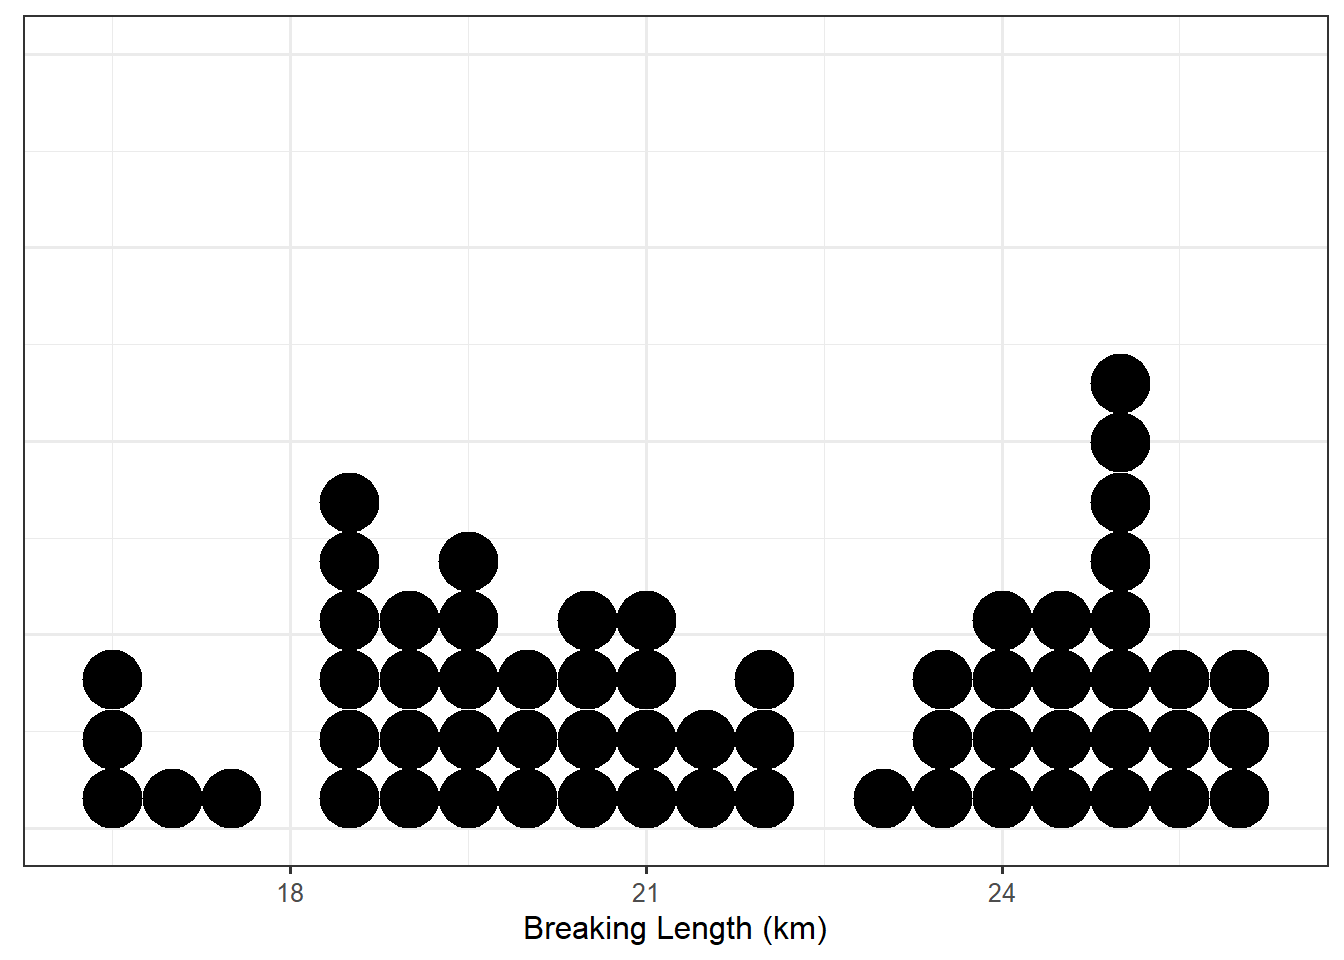
\includegraphics[width=0.8\linewidth]{./Images/summaries-paper-dotplot-1} 

}

\caption{Breaking Length (km) for 62 paper specimens.}\label{fig:summaries-paper-dotplot}
\end{figure}

With any graphic, we tend to be drawn to three components:

\begin{itemize}
\tightlist
\item
  \emph{where} the values tend to be,
\item
  \emph{how tightly} the values tend to be clustered there, and
\item
  \emph{the way} the values tend to cluster.
\end{itemize}

Notice that about half of the paper specimens in the sample had a
breaking length longer than 21.26 km. Only about 25\% of paper specimens
had a breaking length less than 19.33 km. These are measures of
\emph{location}. In particular, these are known as \textbf{percentiles},
of which the \textbf{median}, \textbf{first quartile} and \textbf{third
quartile} are commonly used examples.

\BeginKnitrBlock{definition}[Percentile]
\protect\hypertarget{def:defn-percentile}{}{\label{def:defn-percentile}
\iffalse (Percentile) \fi{} }The \(k\)-th percentile is the value \(q\)
such that \(k\)\% of the values in the distribution are less than or
equal to \(q\). For example,

\begin{itemize}
\tightlist
\item
  25\% of values in a distribution are less than or equal to the 25-th
  percentile (known as the ``first quartile'' and denoted \(Q_1\)).
\item
  50\% of values in a distribution are less than or equal to the 50-th
  percentile (known as the ``median'').
\item
  75\% of values in a distribution are less than or equal to the 75-th
  percentile (known as the ``third quartile'' and denoted \(Q_3\)).
\end{itemize}
\EndKnitrBlock{definition}

The \textbf{average} is also a common measure of location. The breaking
length of a paper specimen is 21.72 km, on average. In this case, the
average breaking length and median breaking length are very close; this
need not be the case. The average is not describing the ``center'' of
the data in the same way as the median; they capture different
properties.

\BeginKnitrBlock{definition}[Average]
\protect\hypertarget{def:defn-average}{}{\label{def:defn-average}
\iffalse (Average) \fi{} }Also known as the ``mean,'' this measure of
location represents the balance point for the distribution. It is
denoted by \(\bar{x}\).

For a sample of size \(n\), it is computed by
\[\bar{x} = \frac{1}{n}\sum_{i=1}^{n} x_i\]

where \(x_i\) rerpesents the \(i\)-th value in the sample.

When referencing the average for a population, the mean is also called
the ``Expected Value,'' and is often denoted by \(\mu\).
\EndKnitrBlock{definition}

Clearly, the breaking length is not equivalent for all paper specimens;
that is, there is variability in the measurements. Measures of
\emph{spread} quantify the variability of values within a distribution.
Common examples include the \textbf{standard deviation} (related to
\textbf{variance}) and \textbf{interquartile range}. For the Paper
Strength example, the breaking length varies with a standard deviation
of 2.88 km; the interquartile range for the breaking length is 5.2 km.

The standard deviation is often reported more often than the variance
since it is on the same scale as the original data; however, as we will
see later, the variance is useful from a mathematical perspective for
derivations. Neither of these values has a natural interpretation;
instead, larger values of these measures simply indicate a higher degree
of variability in the data.

\BeginKnitrBlock{definition}[Variance]
\protect\hypertarget{def:defn-variance}{}{\label{def:defn-variance}
\iffalse (Variance) \fi{} }A measure of spread, this roughly captures
the average distance values in the distribution are from the mean.

For a sample of size \(n\), it is computed by
\[s^2 = \frac{1}{n-1}\sum_{i=1}^{n} \left(x_i - \bar{x}\right)^2\]

where \(\bar{x}\) is the sample mean and \(x_i\) is the \(i\)-th value
in the sample. The division by \(n-1\) instead of \(n\) reduces the bias
in the statistic.

The symbol \(\sigma^2\) is often used to denote the variance in the
population.
\EndKnitrBlock{definition}

\BeginKnitrBlock{definition}[Standard Deviation]
\protect\hypertarget{def:defn-standard-deviation}{}{\label{def:defn-standard-deviation}
\iffalse (Standard Deviation) \fi{} }A measure of spread, this is the
square root of the variance.
\EndKnitrBlock{definition}

\BeginKnitrBlock{definition}[Interquartile Range]
\protect\hypertarget{def:defn-interquartile-range}{}{\label{def:defn-interquartile-range}
\iffalse (Interquartile Range) \fi{} }The distance between the first and
third quartiles. This measure of spread indicates the range over which
the middle 50\% of the data is spread.
\EndKnitrBlock{definition}

The measures we have discussed so far are illustrated in Figure
\ref{fig:summaries-summaries}. While some authors suggest the summaries
you choose to report depends on the shape of the distribution, we argue
that it is best to report the values that align with the question of
interest. It is the question that should be shaped by the beliefs about
the underlying distribution.

\begin{figure}

{\centering 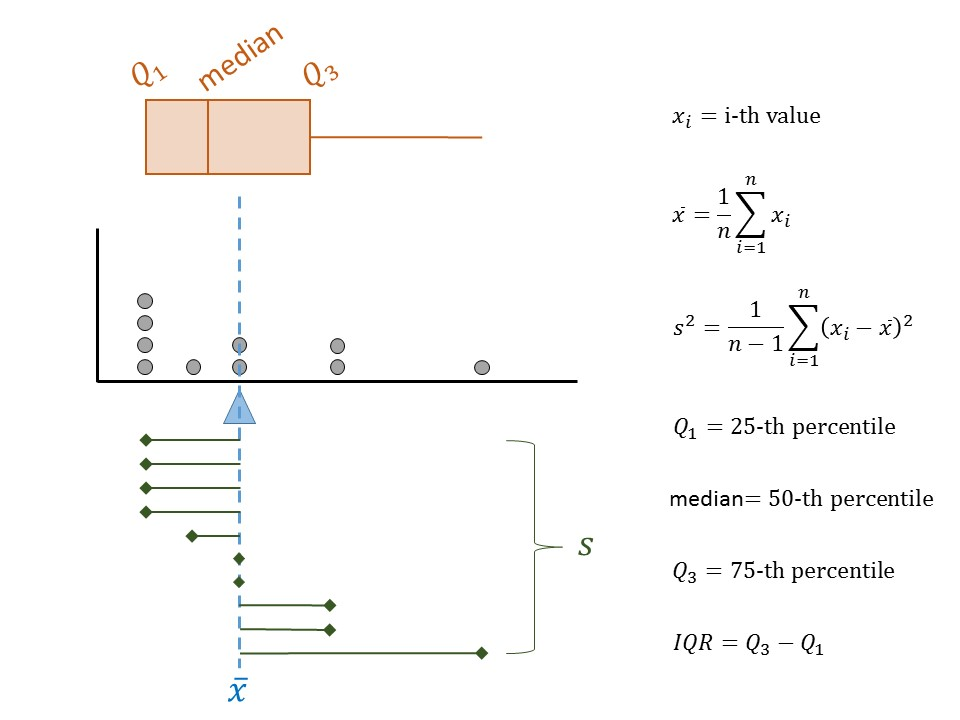
\includegraphics[width=0.8\linewidth]{./images/Summaries-Summaries} 

}

\caption{Illustration of measures of location and spread for a distribution of values.}\label{fig:summaries-summaries}
\end{figure}

Finally, consider the \emph{shape} of the distribution of breaking
length we have observed. The breaking length tends to be clustered in
two locations; we call this \emph{bimodal} (each mode is a ``hump'' in
the distribution). Other terms used to describe the shape of a
distribution are \emph{symmetric} and \emph{skewed}. Symmetry refers to
cutting a distribution in half (at the median) and the lower half being
a mirror image of the upper half; skewed distributions are those which
are not symmetric.

Observe then that the dot plot above gives us some idea of the location,
spread, and shape of the distribution, in a way that the table of values
could not. This makes it a useful graphic as it is characterizing the
\textbf{distribution of the sample} we have observed. This is one of the
four components of what we call the \emph{Distributional Quartet}.

\BeginKnitrBlock{definition}[Distribution of the Sample]
\protect\hypertarget{def:defn-distribution-sample}{}{\label{def:defn-distribution-sample}
\iffalse (Distribution of the Sample) \fi{} }The pattern of variability
in the observed values of a variable.
\EndKnitrBlock{definition}

When the sample is not large, a dot plot is reasonable. Other common
visualizations for a single variable include:

\begin{itemize}
\tightlist
\item
  \emph{jitter plot}: similar to a dot plot, each value observed is
  represented by a dot; the dots are ``jittered'' (shifted randomly) in
  order to avoid overplotting when many subjects share the same value of
  the response.
\item
  \emph{box plot}: a visual depiction of five key percentiles; the plot
  includes the minimum, first quartile, median, third quartile, and
  maximum value observed. The quartiles are connected with a box, the
  median cuts the box into two components.
\item
  \emph{histogram}: can be thought of as a grouped dot plot in which
  subjects are ``binned'' into groups of similar values. The height of
  each bin represents the number of subjects falling into that bin.
\item
  \emph{density plot}: a smoothed histogram in which the y-axis has been
  standardized so that the area under the curve has value 1. The y-axis
  is not interpretable directly, but higher values simply mean more
  likely to occur.
\end{itemize}

To illustrate these graphics, the breaking length for the Paper Strength
example is summarized using various methods in Figure
\ref{fig:summaries-univariate}. The latter three visualizations are more
helpful when the dataset is very large and plotting the raw values
actually hides the distribution. There is no right or wrong graphic; it
is about choosing the graphic which addresses the question and
adequately portrays the distribution.

\begin{figure}

{\centering 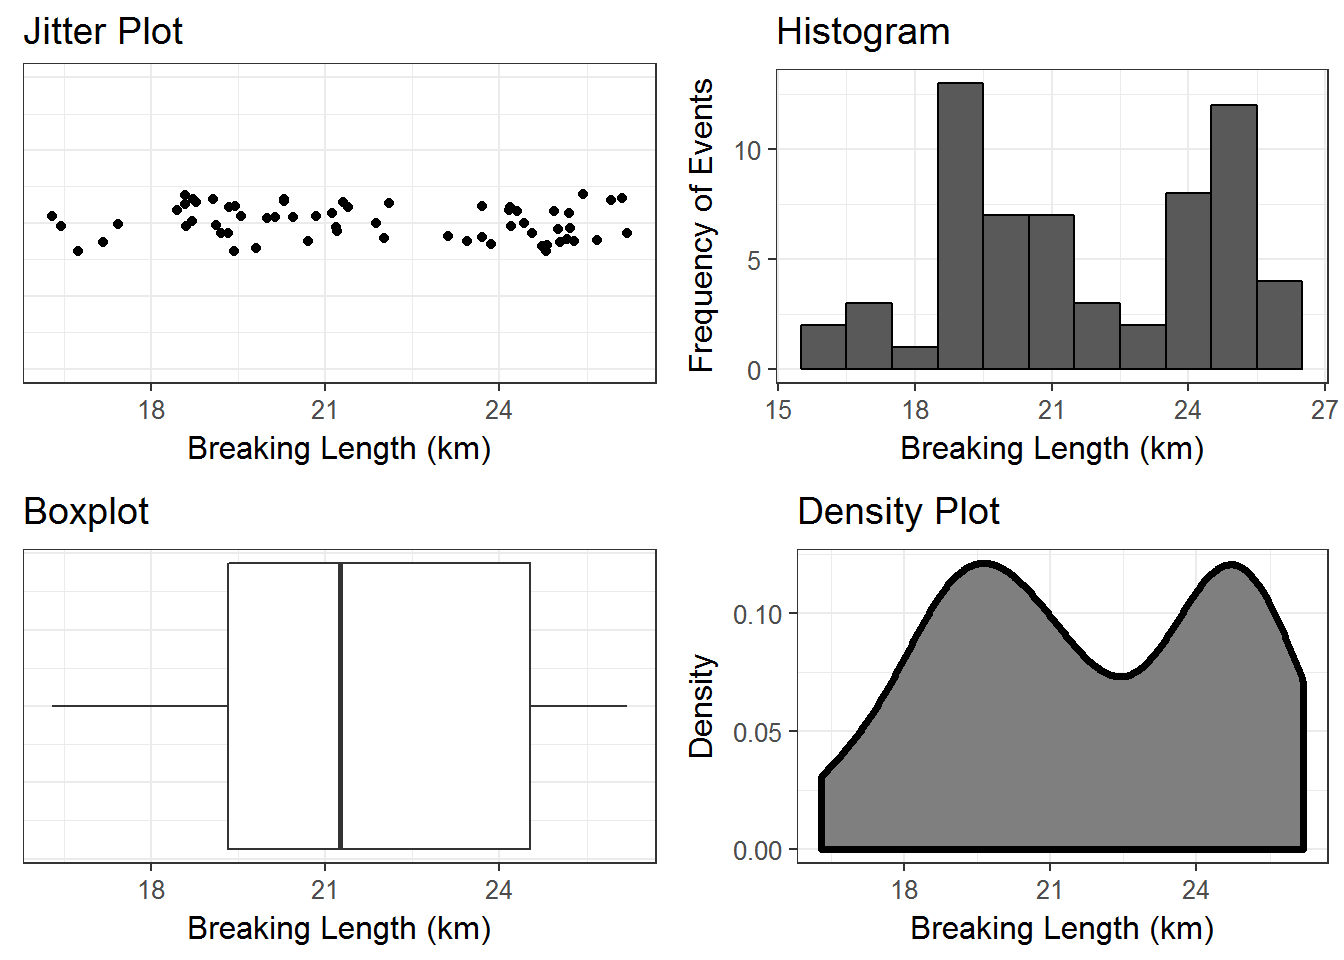
\includegraphics[width=0.8\linewidth]{./Images/summaries-univariate-1} 

}

\caption{Four graphical summaries of the breaking length for the Paper Strength example.}\label{fig:summaries-univariate}
\end{figure}

The numeric summaries of a distribution are known as
\textbf{statistics}. While parameters characterize a variable at the
population level, statistics characterize a variable at the sample
level.

\BeginKnitrBlock{definition}[Statistic]
\protect\hypertarget{def:defn-statistic}{}{\label{def:defn-statistic}
\iffalse (Statistic) \fi{} }Numeric quantity which summarizes the
distribution of a variable within a \emph{sample}.
\EndKnitrBlock{definition}

Why would we compute numerical summaries in the sample if we are
interested in the population? Remember the goal of this discipline is to
use the sample to say something about the underlying population. As long
as the sample is representative, the distribution of the sample should
reflect the \textbf{distribution of the population}; therefore,
summaries of the sample should be close to the analogous summaries of
the population (statistics estimate their corresponding parameters). Now
we see the real importance of having a representative sample; it allows
us to say that what we observe in the sample is a good proxy for what is
happening in the population.

\BeginKnitrBlock{definition}[Distribution of the Population]
\protect\hypertarget{def:defn-distribution-population}{}{\label{def:defn-distribution-population}
\iffalse (Distribution of the Population) \fi{} }The pattern of
variability in values of a variable at the population level. Generally,
this is impossible to know, but we might model it.
\EndKnitrBlock{definition}

That is, the mean in the sample should approximate (estimate) the mean
in the population; the standard deviation of the sample should estimate
the standard deviation in the population; and, the shape of the sample
should approximate the shape of the population, etc. The sample is
acting as a representation in all possible ways of the population.

\BeginKnitrBlock{rmdkeyidea}
A representative sample reflects the population; therefore, we can use
statistics as estimates of the population parameters.
\EndKnitrBlock{rmdkeyidea}

\BeginKnitrBlock{rmdtip}
We would never use \(\bar{x}\) to represent a parameter like the mean of
the population. The symbol \(\bar{x}\) (or \(\bar{y}\), etc.) represents
observed values being averaged together. Since the values are observed,
we must be talking about the sample, and therefore \(\bar{x}\)
represents a statistic. A similar statement could be made for \(s^2\)
(sample variance) compared to \(\sigma^2\) (population variance).

In reality, the symbols themselves are not important. The importance is
on their representation. Statistics are observed while parameters are
not.
\EndKnitrBlock{rmdtip}

\section{Summarizing Relationships}\label{summarizing-relationships}

The summaries discussed above are nice for examining a single variable.
In general, research questions of interest typically involve the
relationship between two or more variables. Most graphics are
two-dimensional (though 3-dimensional graphics and even virtual reality
are being utilized now); therefore, summarizing a rich set of
relationships may require the use of both axes as well as color, shape,
size, and even multiple plots in order to tell the right story. We will
explore these various features in upcoming units of the text. Here, we
focus on the need to tell a story that answers the question of interest
instead of getting lost in making a graphic. Consider the following
question from the \protect\hyperlink{CaseDeepwater}{Deepwater Horizon
Case Study}:

\begin{quote}
What is the increased risk of developing adverse respiratory symptoms
for volunteers cleaning wildlife compared to those volunteers who do not
have direct exposure to oil?
\end{quote}

Consider the graphic in Figure \ref{fig:summaries-bad-barchart}; this is
\emph{not} a useful graphic. While it compares the number of volunteers
with symptoms in each group, we cannot adequately address the question
because the research question involves comparing the rates for the two
groups.

\begin{figure}

{\centering 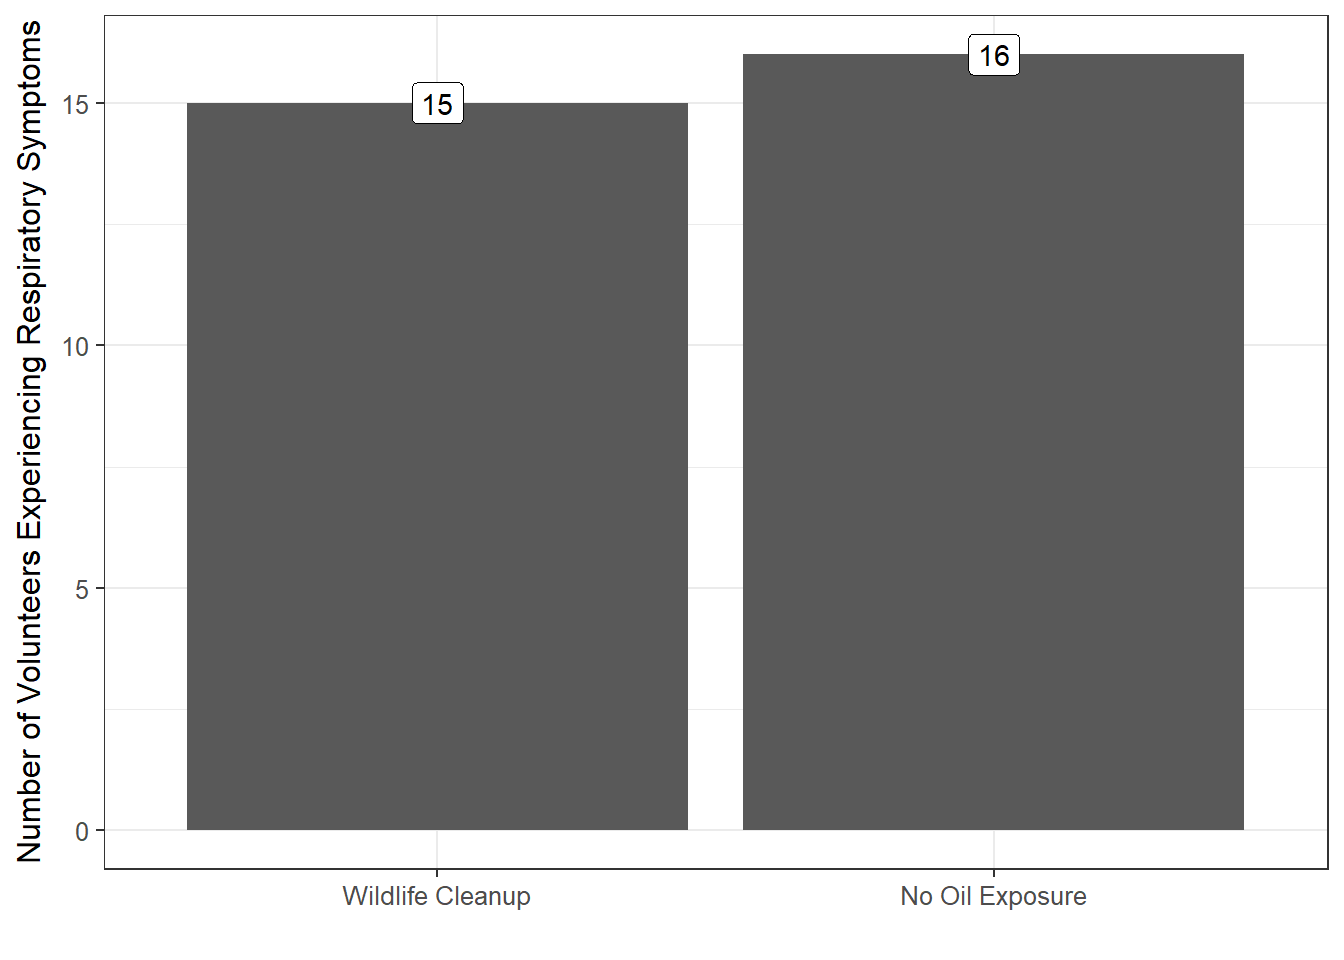
\includegraphics[width=0.8\linewidth]{./Images/summaries-bad-barchart-1} 

}

\caption{Illustration of a poor graphic; the graphic does not give us a sense of the rate within each group in order to make a comparison.}\label{fig:summaries-bad-barchart}
\end{figure}

Instead, Figure \ref{fig:summaries-good-barchart} compares the rates
within each group. Notice that since we are reporting relative
frequencies, we also report the sample size for each group.

\begin{figure}

{\centering 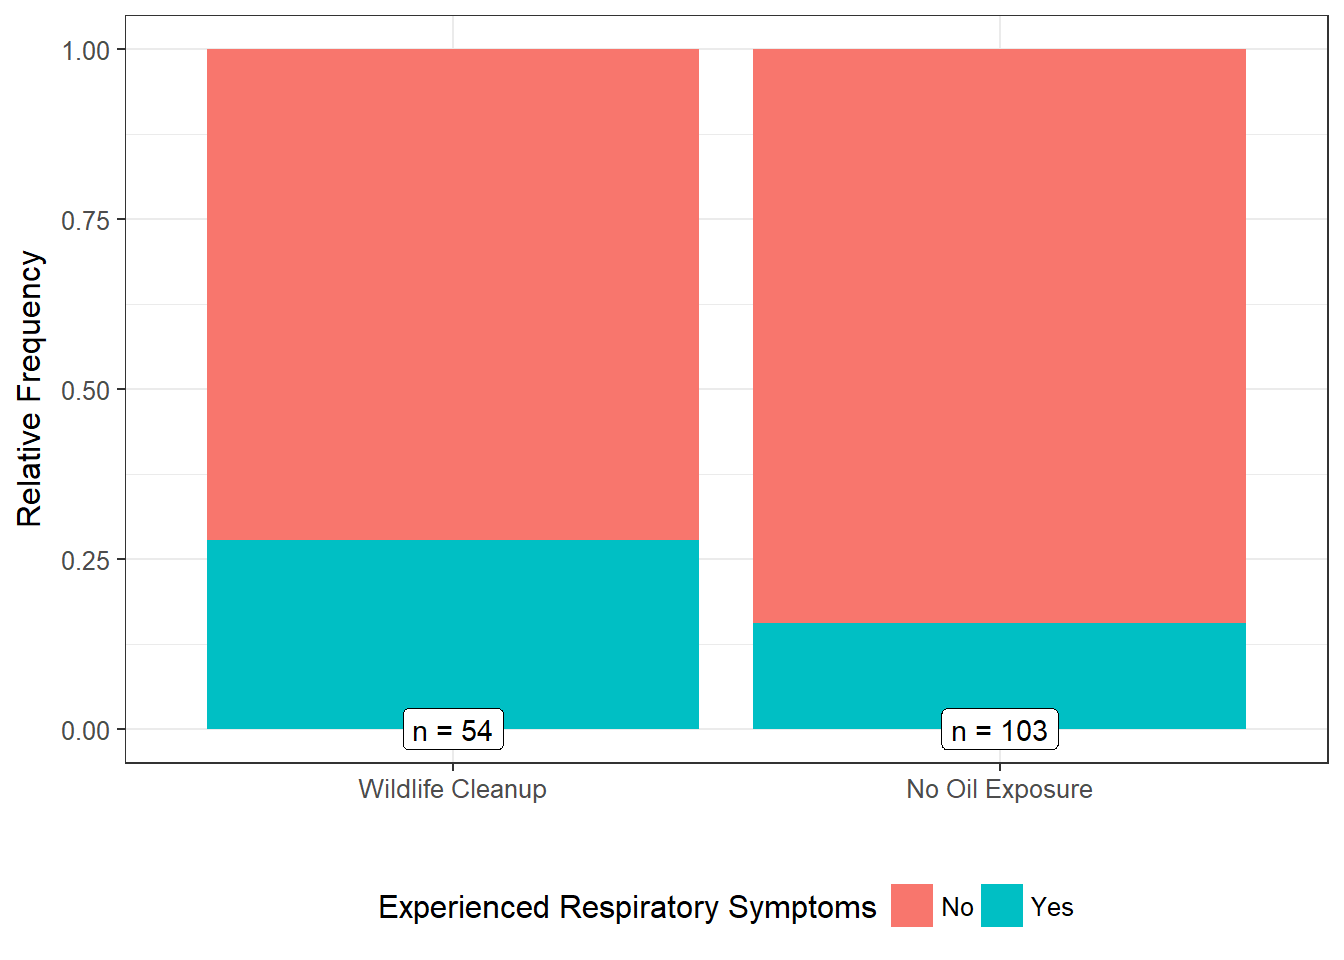
\includegraphics[width=0.8\linewidth]{./Images/summaries-good-barchart-1} 

}

\caption{Comparison of the rate of adverse respiratory symptoms among volunteers assigned to different tasks.}\label{fig:summaries-good-barchart}
\end{figure}

From the graphic, it becomes clear that within the sample a higher
fraction of volunteers cleaning wildlife experienced adverse symptoms
compared with those without oil exposure. In fact, volunteers cleaning
wildlife were 1.79 times more likely to experience adverse respiratory
symptoms.

The key to a good summary is understanding the question of interest and
addressing this question through a useful characterization of the
variability.

\chapter{Assessing the Evidence (Quantifying the Variability in
Estimates)}\label{SamplingDistns}

Again, the goal of statistical inference is to use the sample as a
snapshot of the underlying population (Figure
\ref{fig:samplingdistns-statistical-process}). There are generally three
reasons people distrust this process:

\begin{enumerate}
\def\labelenumi{\arabic{enumi}.}
\tightlist
\item
  Fear that the sample does not represent what is going on in the
  population.
\item
  Fear that we cannot make a conclusion with a sample of size \(n\)
  (wanting more data).
\item
  Fear that one study is not enough to make a conclusion.
\end{enumerate}

\begin{figure}

{\centering 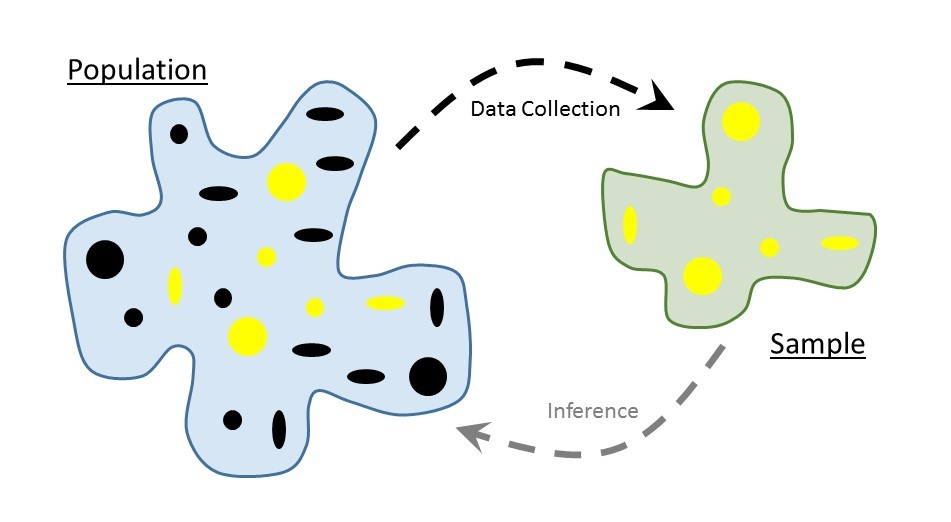
\includegraphics[width=0.8\linewidth]{images/Basics-Stat-Process} 

}

\caption{Illustration of the statistical process (reprinted from Chapter 1).}\label{fig:samplingdistns-statistical-process}
\end{figure}

We have already tackled the first fear in Chapter \ref{Data}; if we are
to trust statistical results, we must collect data that is
representative of the underlying population. The second and third fears
above are tied together, though maybe not obviously. Before launching
into a slightly more formal discussion, consider the following thought
experiment.

\BeginKnitrBlock{example}[Free Throws]
\protect\hypertarget{exm:samplingdistns-free-throws}{}{\label{exm:samplingdistns-free-throws}
\iffalse (Free Throws) \fi{} }Your friend Dave lives for his Wednesday
``pick-up'' basketball games at the gym. One afternoon, while waiting
for a few more players to arrive Dave shoots 10 free throws, of which he
makes 3.
\EndKnitrBlock{example}

I imagine no one is ready to claim \emph{definitively} that Dave has a
30\% success rate from the free throw line. So, what can we say? Well,
if this set of 10 free throws is representative of Dave's free throw
performance, then we would say that 30\% is an \emph{estimate} for his
success rate; that is, the statistic 30\% is a good guess at the unknown
parameter (overall success rate). There are two ways we might impove our
confidence in this estimate. First, we might consider a larger sample
size (make Dave shoot more free throws); let's continue along these
lines for a moment.

\BeginKnitrBlock{example}[Free Throws (cont.)]
\protect\hypertarget{exm:samplingdistns-free-throws2}{}{\label{exm:samplingdistns-free-throws2}
\iffalse (Free Throws (cont.)) \fi{} }Joe has also been waiting for a
few more players to arrive; however, Joe shoots 100 free throws (clearly
he has more time on his hands) of which he makes 30.
\EndKnitrBlock{example}

Again, we probably wouldn't claim \emph{definitively} that Joe has a
30\% success rate from the free throw line. And again, assuming this set
of 100 free throws is representative of his overall performance, we
would say 30\% is an \emph{estimate} for his success rate. But, we would
also say we are more confident in our guess for Joe's overall
performance compared with our guess for Dave's. The more shots we
observe, the more confidence we have in our estimate. This idea is known
as the \textbf{Law of Large Numbers}.

\BeginKnitrBlock{definition}[Law of Large Numbers]
\protect\hypertarget{def:defn-lln}{}{\label{def:defn-lln} \iffalse (Law of
Large Numbers) \fi{} }For our purposes, this essentially says that as a
sample size gets infinitely large, a statistic will become arbitrarily
close (extremely good approximation) of the parameter it estimates.
\EndKnitrBlock{definition}

There are two drawbacks with the Law of Large Numbers. First, it does
not tell us how ``close'' a statistic is to the parameter for any
specific sample size; second, we cannot take an infinitely large sample.
And, for populations which are infinitely large (like all the free
throws Dave could ever shoot, for example), any sample size could be
considered small relative to the size of the population. For our thought
experiment, it is probably not feasible to have Dave or Joe shoot
thousands of free throws, for example. Our goal then becomes to somehow
quantify the confidence we have in our estimates \emph{given the sample
size we have available}. That is, given that we only saw Dave shoot 10
free throws, can we quantify our confidence in that 30\% estimate of his
free throw success? Of course, we need to know what we mean by
``confidence.''

\BeginKnitrBlock{rmdkeyidea}
In statistics, our ``confidence'' in an estimate is tied to the
estimate's repeatability --- ``if we were to repeat the study, how much
would we expect our estimate to change?''
\EndKnitrBlock{rmdkeyidea}

This notion of confidence gets at the last fear. We know that if we
repeat a study, the results will change; our job is to quantify (keeping
the sample size in mind) the degree to which the results will change.
That is, we need to quantify the \emph{variability} in the estimate
across repeated studies (known as sampling variability; we told you
statistics was all about variability). This is characterized by the
\textbf{sampling distribution}.

\BeginKnitrBlock{definition}[Sampling Distribution]
\protect\hypertarget{def:defn-sampling-distribution}{}{\label{def:defn-sampling-distribution}
\iffalse (Sampling Distribution) \fi{} }The distribution of a
\emph{statistic} across repeated samples.
\EndKnitrBlock{definition}

This is perhaps the most important of the \emph{Distributional Quartet};
it is the holy grail of statistical inference. Once we have the sampling
distribution, inference is straight-forward.

\BeginKnitrBlock{rmdfivefund}
\textbf{Fundamental Idea IV}: Variability is inherent in any process,
and as a result, our estimates are subject to sampling variability.
However, these estimates often vary across samples in a predictable way;
that is, they have a distribution that can be modeled.
\EndKnitrBlock{rmdfivefund}

\section{Conceptualizing the Sampling
Distribution}\label{conceptualizing-the-sampling-distribution}

The sampling distribution of a statistic is one of the most fundamental,
and yet one of the most abstract, concepts in statistics. Its name is
even confusing; the ``distribution of the sample'' (Definition
\ref{def:defn-distribution-sample}) and the ``sampling distribution''
(Definition \ref{def:defn-sampling-distribution}) are two different
things. Let's first focus on getting ahold of this abstract concepts.

For the \protect\hyperlink{DeepwaterCase}{Deepwater Horizon Case Study},
consider the following question:

\begin{quote}
What proportion of volunteers assigned to clean wildlife will develop
adverse respiratory symptoms?
\end{quote}

In the sample, we observed 15 out of 54 such volunteers (27.8\% or a
proportion of 0.278). This proportion is a good estimate of the rate of
adverse symptoms in the population (assuming the sample is
representative, of course).

Now, imagine randomly selecting 54 \emph{new} volunteers from the
population (repeating the study). For this new sample, it would be
possible to determine the fraction of volunteers that experienced
adverse symptoms; we would expect this value to be a bit different than
what we obtained in the first sample since the two samples consist of
different subjects. Since this second sample is also representative,
however, it also provides a good estimate of the parameter. That is, we
now have two good estimates of the same parameter.

Now, we could take a third random sample of 54 volunteers and compute
the fraction in this third sample which experienced adverse symptoms.
This third sample also provides a good (and potentially unique) estimate
of the parameter. We could continue this process \(m\) times, for some
large number \(m\), as illustrated in Figure
\ref{fig:samplingdistns-sampling-distribution}.

\begin{figure}

{\centering 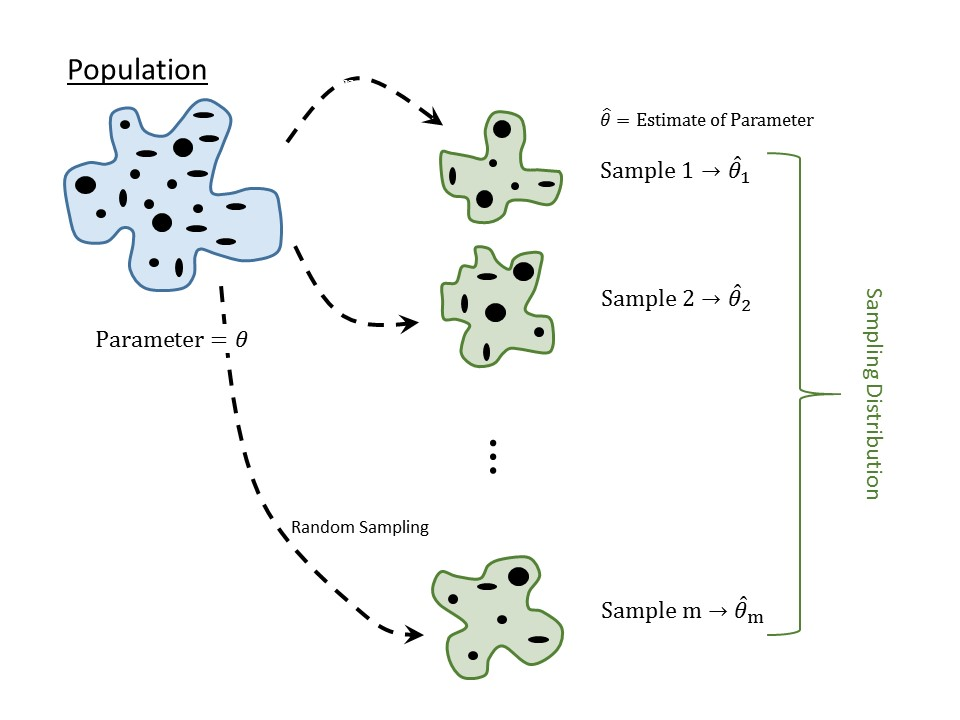
\includegraphics[width=0.8\linewidth]{./images/SamplingDistns-Sampling-Distribution} 

}

\caption{Illustration of repeatedly sampling from a population.}\label{fig:samplingdistns-sampling-distribution}
\end{figure}

Consider what we are describing. With each representative sample, we
have constructed an estimate of the parameter. What we have kept from
each replicate sample is \emph{not} the values of the variables
themselves (whether the volunteers experienced adverse respiratory
symptoms); instead, we have retained the \emph{statistic} from each of
\(m\) completely different studies. So, which of these \(m\) estimates
do we trust? \emph{All of them.} Since each sample is representative of
the population, each estimate is a good (not perfect) estimate of the
parameter. Since we have all these estimates, we could think about
pooling the information from all of them; describing the way in which
these estimates change from one sample to another is the sampling
distribution.

Notice that the sampling distribution is not describing a variable; it
is describing a \emph{statistic}. In order to construct a sampling
distribution, we go through the following steps:

\begin{enumerate}
\def\labelenumi{\arabic{enumi}.}
\tightlist
\item
  Take a sample; record variables of interest.
\item
  Compute the statistic which estimates the parameter and retain this
  value.
\item
  Repeat steps 1 and 2 a large number of times.
\item
  Examine the statistics collected.
\end{enumerate}

So, the sampling distribution is not a plot of the raw values of a
variable on individual subjects but a plot of statistics which summarize
entire samples. That is, the unit of observation has changed. While a
sample consists of individual subjects from the population, the sampling
distribution consists of individual samples from the population.

\BeginKnitrBlock{rmdtip}
Re-read the description of a sampling distribution several times, and
return to it often as you read through the text. It takes a while for
this to sink in, but if you truly grasp this one concept, the remainder
of statistical inference becomes much more accessible.
\EndKnitrBlock{rmdtip}

\section{Example of a Sampling
Distribution}\label{example-of-a-sampling-distribution}

Since this idea is so critical to grasping statistical inference, we are
going to walk through the process of generating a sampling distribution
for a known data generating process.

\BeginKnitrBlock{example}[Dice Experiment]
\protect\hypertarget{exm:samplingdistns-dice}{}{\label{exm:samplingdistns-dice}
\iffalse (Dice Experiment) \fi{} }Consider an ordinary six-sided die; we
are interested in the proportion of times that rolling the die will
result in a 1. Putting this in the language of the statistics, we have
the following:

\begin{itemize}
\tightlist
\item
  The \emph{population} of interest is all rolls of the die. Notice that
  this population is infinitely large as we could roll the die forever.
\item
  The \emph{variable} is the resulting value from the roll. Since this
  can take on only one of six values, this is a categorical variable.
\item
  The \emph{parameter} of interest is the proportion of rolls that
  result in a 1.
\end{itemize}

Our goal is to construct the sampling distribution of the \emph{sample
proportion} of rolls that result in a 1 when the die is rolled 20 times.
\EndKnitrBlock{example}

What makes this example unique is that we know the value of the
parameter. Because of the physical properties of a die, we know that the
probability a roll results in a 1 is \(\theta = 1/6\). So, statistical
inference is not needed here. This example simply provides a simple
vehicle for studying sampling distributions. Also, before going on,
notice that the sampling distribution is for the statistic (the
\emph{sample proportion}) and not the parameter; and, it is constructed
for a fixed sample size (in this case, \(n = 20\) rolls). Going back to
the steps for creating a sampling distribution described in the previous
section, we have the following steps:

\begin{enumerate}
\def\labelenumi{\arabic{enumi}.}
\tightlist
\item
  Roll a die 20 times, each time recording the resulting value.
\item
  Compute the proportion of times (out of the 20) the resulting value
  was a 1 and retain this value.
\item
  Repeat steps 1 and 2 a large number of times (let's say 500).
\item
  Plot the resulting values; there should be 500 proportions that we are
  keeping.
\end{enumerate}

Notice that we are actually rolling a die 10000 times (20 rolls repeated
500 times); we only keep 500 values (one proportion for each set of 20
rolls). This is something you could physically do at home. For example,
the first sample might look like that in Figure
\ref{fig:samplingdistns-dice-example}.

\begin{figure}

{\centering 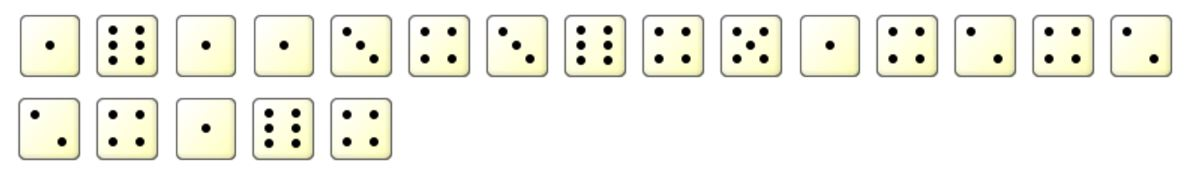
\includegraphics[width=0.8\linewidth]{./images/SamplingDistns-Dice-Example} 

}

\caption{Potential sample of rolling a die 20 times.}\label{fig:samplingdistns-dice-example}
\end{figure}

For this particular sample, the proportion in the sample (our statistic
of interest) would be 0.25 (\(5/20\)). That is the value we would
record. We then repeat this 499 more times. You could try a few out
yourself using \href{https://www.random.org/dice/?num=20}{an online
simulator}. Figure \ref{fig:samplingdistns-dice-dotplot} shows the
resulting proportions for when we simulated this process with 500
samples, each sample consisting of 20 rolls.

\begin{figure}

{\centering 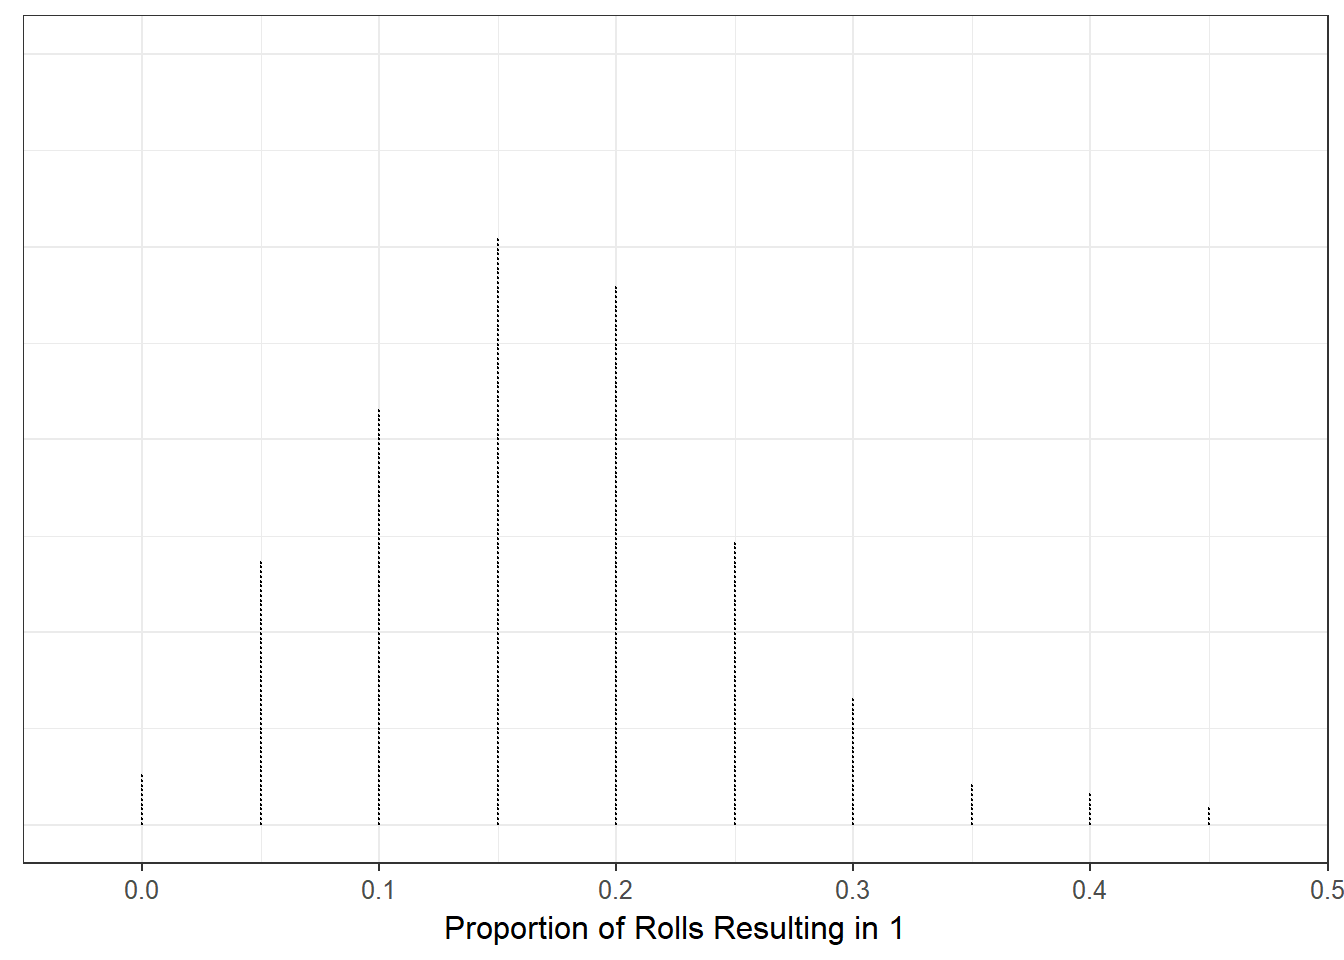
\includegraphics[width=0.8\linewidth]{./Images/samplingdistns-dice-dotplot-1} 

}

\caption{Sampling distribution for the proportion of 20 rolls of a die which result in a 1.  The distribution is based on repeating the sampling process 500 times.}\label{fig:samplingdistns-dice-dotplot}
\end{figure}

With modern computing power, there is no need to restrain ourselves to
repeating the study 500 times. A simple computer program could replicate
rolling the study (20 rolls of a die) thousands of times. Figure
\ref{fig:samplingdistns-dice-histogram} is the sampling distribution for
the proportion of rolls that result in a 1 based on a sample of size 20,
repeating the study 50000 times.

\begin{figure}

{\centering 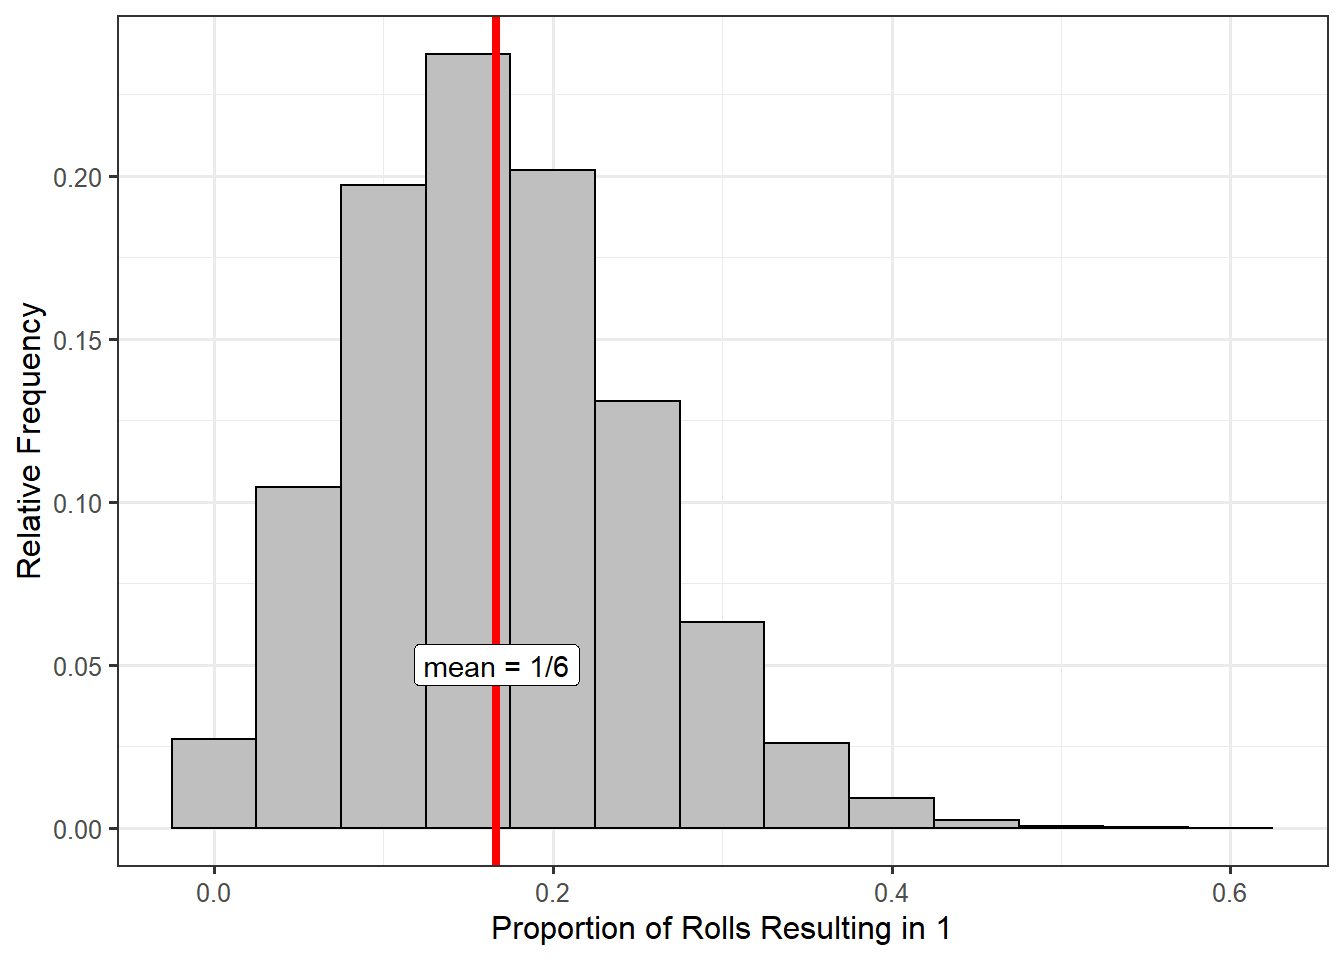
\includegraphics[width=0.8\linewidth]{./Images/samplingdistns-dice-histogram-1} 

}

\caption{Sampling distribution for the proportion of 20 rolls of a die which result in a 1.  The distribution is based on repeating the sampling process 50000 times.}\label{fig:samplingdistns-dice-histogram}
\end{figure}

Notice that the sampling distribution is centered around the true value
of the parameter (\(\theta = 1/6\)). In general, the sampling
distribution of a statistic, when taken from a random sample, is
centered on the true value of the parameter. This is the unbiased nature
of the data coming out; random samples are representative of the
population. Similarly, note that while no one sample (remember, each
value in the distribution represents a statistic from a sample of 20
values) is perfect, none of the samples produced values which were
really far from the true parameter. That is, a representative sample may
not be perfect, but it will give a \emph{reasonable} estimate of the
parameter. Notice that these properties hold even though we had a
relatively small sample size (only rolling the die \(n = 20\) times).

\BeginKnitrBlock{rmdkeyidea}
The size of the sample is not as important as whether it is
representative. A small representative sample is better for making
inference than a large sample which is biased.
\EndKnitrBlock{rmdkeyidea}

One of the most useful things about the sampling distribution is that it
gives us an idea of how much we might expect our statistic to change
from one sample to another. Based on Figure
\ref{fig:samplingdistns-dice-histogram}, we could say that if we roll a
die 20 times, the proportion of rolls which result in a 1 is most likely
to be between 0.05 and 0.30 (so somewhere between 1 and 6 ones out of
the 20 rolls). It would be \emph{extremely} rare to have 12 of the 20
rolls result in a 1 (notice how small the bar is on the 0.6 proportion).
The sampling distribution is therefore giving us an idea of the
variability in our statistic.

Remember, our goal was to account for the variability in the statistic
(how much it changes from one sample to another) \emph{while accounting
for the sample size}. How is this done? When forming the sampling
distribution, we repeated the study. For each replication, we obtained a
new sample that \emph{had the same size as the original}. So, the sample
size is baked into the sampling distribution. To see the impact of
taking a larger sample, consider rolling a six-sided die 60 times
instead of 20 times. When we build the sampling distribution, each
replication will then involve repeating the process with 60 new rolls.
Figure \ref{fig:samplingdistns-dice-histogram2} shows the sampling
distribution of the proportion of 60 rolls which result in a 1, using
50000 replications. Notice that the distribution is still centered on
the true parameter \(\theta = 1/6\). The primary difference between this
figure and the last is that when we increased the sample size, the
sampling distribution narrowed.

\begin{figure}

{\centering 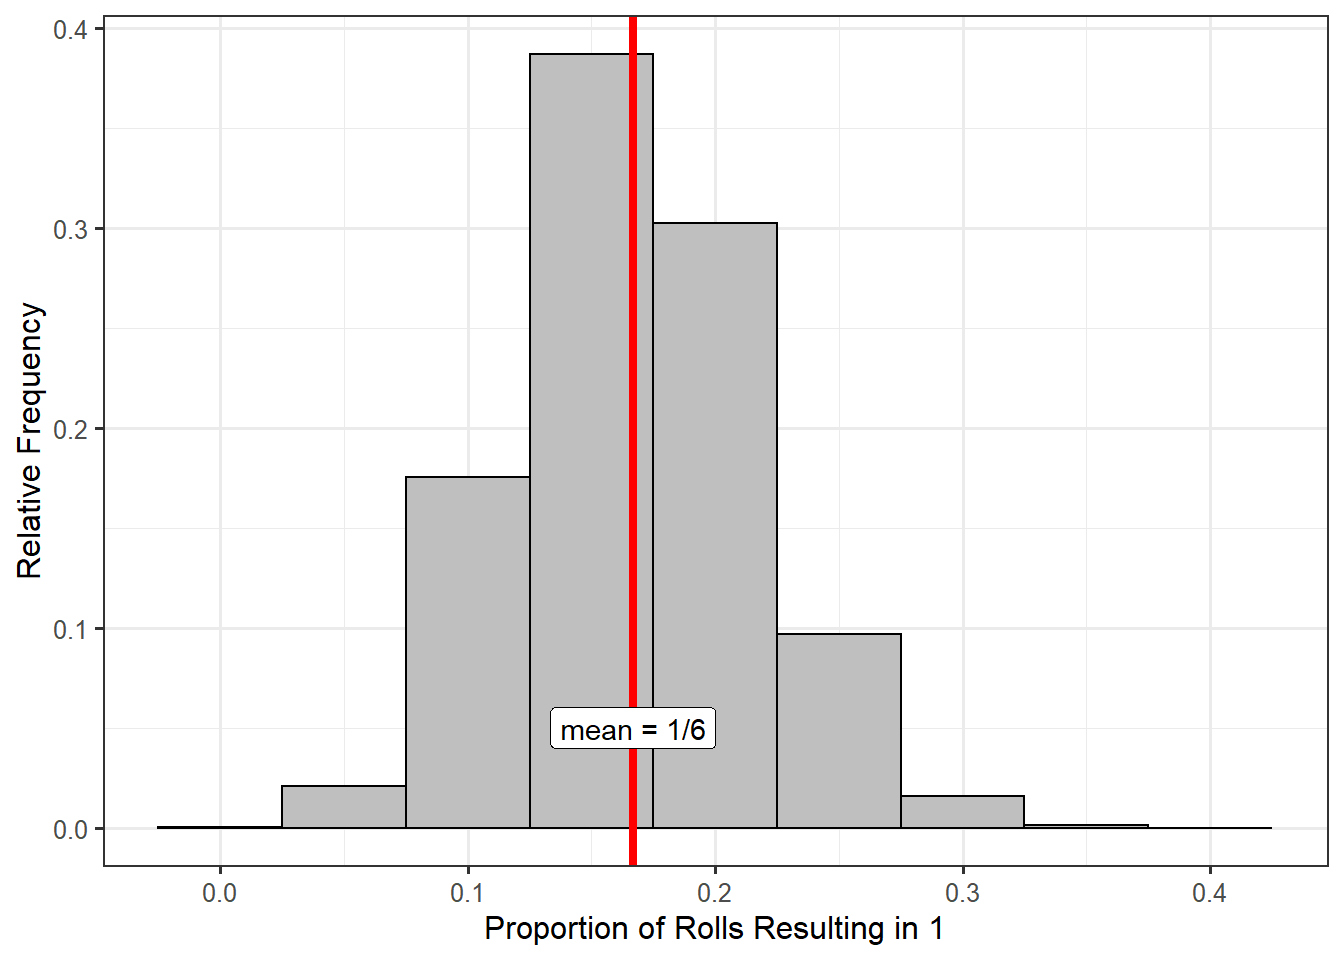
\includegraphics[width=0.8\linewidth]{./Images/samplingdistns-dice-histogram2-1} 

}

\caption{Sampling distribution for the proportion of 60 rolls of a die which result in a 1.  The distribution is based on repeating the sampling process 50000 times.}\label{fig:samplingdistns-dice-histogram2}
\end{figure}

We all have this intuition that ``more data is better.'' In truth, we
should say ``more \emph{good} data is better.'' By ``better,'' we mean
that the statistic is less variable. Notice that we have to be careful
here. We are not saying that the \emph{sample} has less variability; we
are saying the \emph{statistic} has less variability. That is, we are
more confident in our estimate because we do not expect it to change as
much from one sample to the next. From Figure
\ref{fig:samplingdistns-dice-histogram2}, we have that if we roll the
die 60 times, we expect the proportion of 1's to be somewhere between
0.1 and 0.25 (somewhere between 6 and 15 ones out of the 60 show up).
The proportion is varying much less from one sample to the next compared
to when we rolled the die only 20 times.

\BeginKnitrBlock{rmdkeyidea}
Larger samples result in \emph{statistics} which are less variable. This
shows itself in the sense that the sampling distribuiton is narrower.
\EndKnitrBlock{rmdkeyidea}

\BeginKnitrBlock{rmdtip}
Students often believe that a large sample reduces the variability in
the data. That is not true; a large sample reduces the variability in
the \emph{statistic}.
\EndKnitrBlock{rmdtip}

\section{Modeling the Sampling
Distribution}\label{modeling-the-sampling-distribution}

Let's return to the \protect\hyperlink{CaseDeepwater}{Deepwater Horizon
Case Study}. In particular, suppose we are tyring to address the
following question:

\begin{quote}
What proportion of volunteers assigned to clean wildlife will develop
adverse respiratory symptoms?
\end{quote}

We have an estimate for this proportion (\(\widehat{p} = 0.278\)) based
on the observed sample. Based on the discussion in the previous section,
we know the sampling distribution of this proportion can help us
quantify the variability in the estimate. Figure
\ref{fig:samplingdistns-deepwater-histogram} represents the sampling
distribution of this proportion. From the graphic, we would not expect
the proportion of volunteers who experience adverse respiratory symptoms
to move much beyond 0.15 and 0.4 if we were to repeat the study; it
would almost certainly not move beyond 0.1 and 0.5 if we were to repeat
the study.

\begin{figure}

{\centering 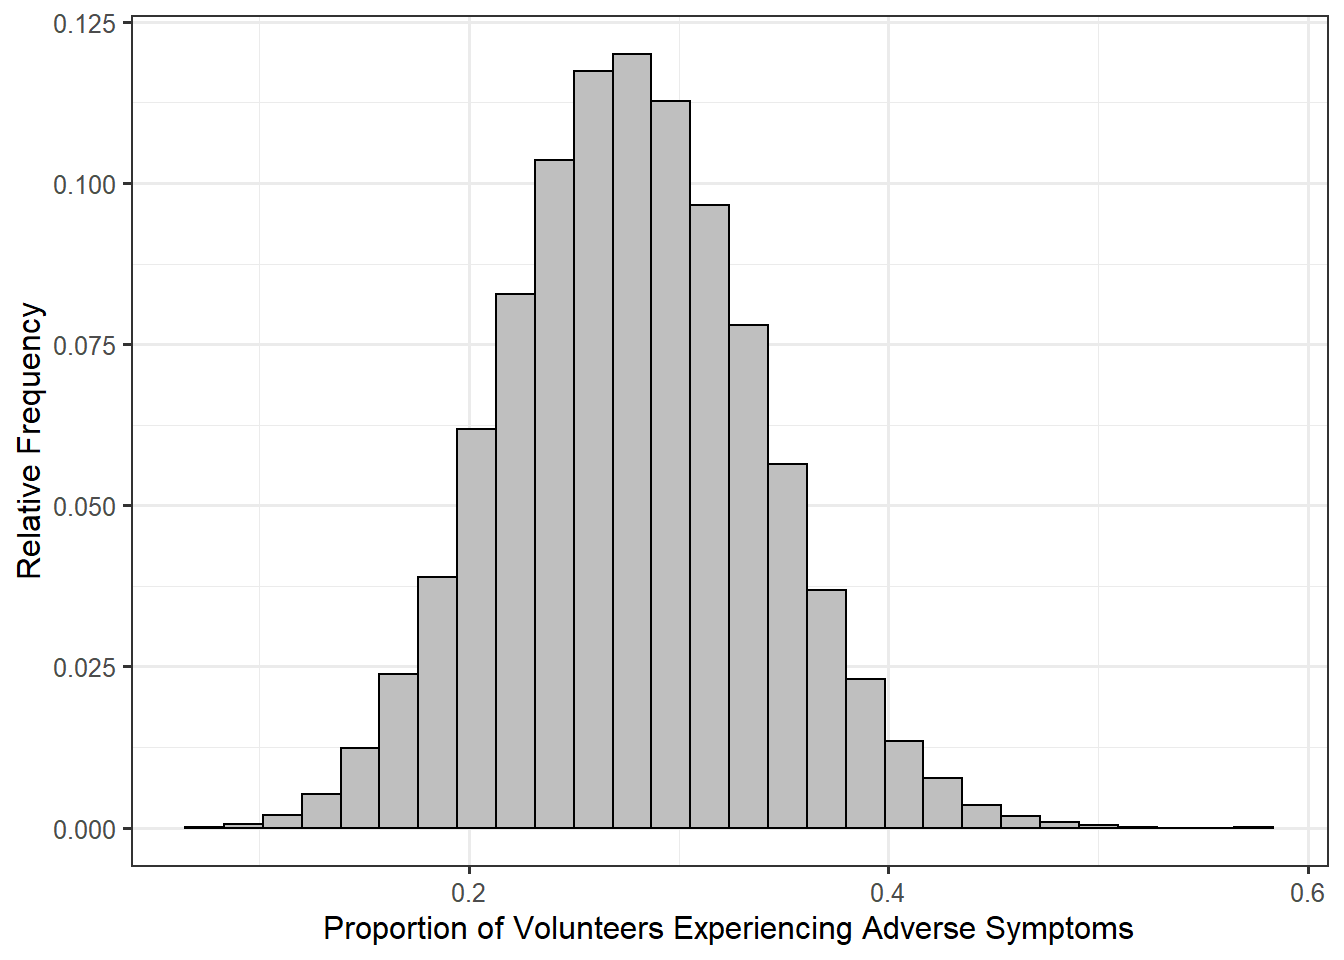
\includegraphics[width=0.8\linewidth]{./Images/samplingdistns-deepwater-histogram-1} 

}

\caption{Sampling distribution for the proportion of volunteers assigned to wildlife who will develop adverse symptoms based on a sample of 54 volunteers.}\label{fig:samplingdistns-deepwater-histogram}
\end{figure}

Now, you might ask ``wait, where did this sampling distribution come
from? There is no way you actually repeated the study 50000 times,
right?'' Right. In the previous section, we described building the
sampling distribution through repeated sampling. But, in practice, this
is never practical; if it were, we would have just conducted a bigger
sample to begin with. Generally, cost is the limiting factor in choosing
a sample size; so, we only have a limited set of data to work with. The
sampling distribution is critical to making inference, but we cannot
take multiple samples to make it. Where does that leave us? The
answer\ldots{}modeling. Our goal is to construct a \emph{model} of the
sampling distribution that we can use to make inference.

There are three general techniques for modeling the sampling
distribution of a statistic:

\begin{enumerate}
\def\labelenumi{\arabic{enumi}.}
\tightlist
\item
  Build an empirical model.
\item
  Build an exact analytical model using probability relations.
\item
  Build an approximate analytical model using probability limit
  theorems.
\end{enumerate}

We will focus on the first approach; the latter two approaches are
discussed in the last unit of the text. Our emphasis is on the
conceptual understanding of a sampling distribution and its model. While
these latter two approaches differ in their technique, the use of the
resulting model is the same. We choose to focus on the first approach
because it requires less background and reinforces the conceptual
understanding of a sampling distribution discussed above. The idea in
constructing an empirical model is to mimic the discussion above
regarding the construction of a sampling distribution. Our description
references Figure \ref{fig:samplingdistns-bootstrap} often.

We are limited by our resources; because of time and money constraints,
we cannot resample from the population (crossed off resamples in Figure
\ref{fig:samplingdistns-bootstrap}). So, we pretend for a moment that
our original sample (colored in green in the figure) is the population
for a moment. Our idea is to randomly sample from this original sample,
creating a \emph{resample} (colored in orange in the figure). Forgive
the non-technical terms here, but since the orange ``blob'' is a random
sample from the green ``blob,'' then it is representative of the green
blob. Therefore, if we construct an estimate \(\widehat{\theta}^*\) from
the orange blob (the star denotes a statistic from a resample), then it
should be close to the statistic \(\widehat{\theta}\) from the green
blob; but, since this green blob is representative of the population,
\(\widehat{\theta}\) should be close to the true parameter \(\theta\).
Therefore, we have that \[
\widehat{\theta}^* \approx \widehat{\theta} \approx \theta \Rightarrow \widehat{\theta}^* \approx \theta
\]

That is, each resample produces a statistic which is a good estimate of
the parameter from the underlying population. The benefit here is that
the resamples are from the original sample, not the population, and can
therefore be constructed in the computer. And, given today's computing
power, we are not limited by time or money (10000 resamples can often be
taken in a matter of seconds). If you want to see this process in
action, we encourage you to check out the free online app located at
\url{http://www.lock5stat.com/StatKey/bootstrap_1_cat/bootstrap_1_cat.html}.

\begin{figure}

{\centering 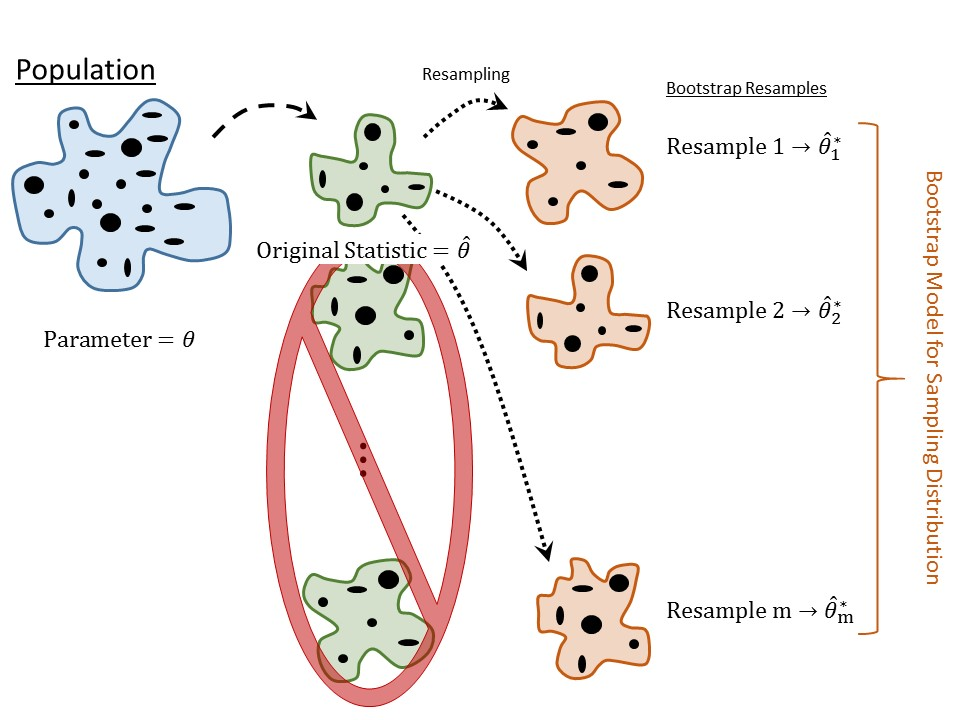
\includegraphics[width=0.8\linewidth]{./images/SamplingDistns-Bootstrap} 

}

\caption{Illustration of modeling the sampling distribution via the Bootstrap.}\label{fig:samplingdistns-bootstrap}
\end{figure}

Again, the idea is to mimic in the computer the resampling that we were
unable to do in real life. This process is known as the
\textbf{bootstrap} procedure.

\BeginKnitrBlock{definition}[Bootstrap]
\protect\hypertarget{def:defn-bootstrap}{}{\label{def:defn-bootstrap}
\iffalse (Bootstrap) \fi{} }A method of modeling the sampling
distribution by repeatedly resampling from the original data.
\EndKnitrBlock{definition}

A couple of notes on the actual implementation of a bootstrap procedure:

\begin{enumerate}
\def\labelenumi{\arabic{enumi}.}
\tightlist
\item
  Each resample (known as a \emph{bootstrap resample}) is the same size
  as the original sample.
\item
  Each resample is taken \emph{with replacement}; that means the values
  from the original sample can show up multiple times. Think of ``catch
  and release'' fishing.
\item
  Typically, between 3000 and 10000 bootstrap resamples are taken.
\end{enumerate}

We will avoid actual computation throughout the text, but several
resources are available for implementing the bootstrap procedure (and
its many variants) in various computer programming languages and
software packages.

\BeginKnitrBlock{rmdtip}
Students often believe that the bootstrap ``creates more data.'' This is
not true. Instead, the boostrap resamples from the existing data. This
highlights the need to have a representative sample when performing
analysis.
\EndKnitrBlock{rmdtip}

As an example, for the \protect\hyperlink{CaseDeepwater}{Deepwater
Horizon Case Study}, we performed the following steps to create Figure
\ref{fig:samplingdistns-deepwater-histogram}:

\begin{enumerate}
\def\labelenumi{\arabic{enumi}.}
\tightlist
\item
  Select 54 volunteers at random (with replacement) from the original
  sample of 54 volunteers who had been assigned to clean wildlife.
\item
  For our bootstrap resample, we compute the proportion of those
  individuals who had experienced adverse respiratory symptoms; this is
  our \emph{bootstrap statistic}.
\item
  We repeated steps 1 and 2 several thousand times, retaining the
  bootstrap statistics from each bootstrap resample.
\item
  We plotted the distribution of the bootstrap statistics.
\end{enumerate}

\section{Using a Model for the Sampling Distributions (Confidence
Intervals)}\label{using-a-model-for-the-sampling-distributions-confidence-intervals}

In Chapter \ref{Summaries} we discussed specific statistics, numerical
estimates of our parameters. Returning to our question for the
\protect\hyperlink{CaseDeepwater}{Deepwater Horizon Case Study} ---
``What proportion of volunteers assigned to clean wildlife will develop
adverse respiratory symptoms?'' --- we have such an estimate:
\(\widehat{p} = 0.278\). However, there is something unsatisfying about
this estimate\ldots{}it fails to acknowledge the variability in the
statistic which we know exists. We would like to leverage the
information contained in our model for the sampling distribution to
provide an estimate which incorporates the variability in this
statistic.

From Figure \ref{fig:samplingdistns-deepwater-histogram}, we observed
that we would not expect the proportion of volunteers who had
experienced adverse symptoms to move much beyond 0.15 to 0.4 if we were
to repeat the study. How does this help us in performing inference?
Remember that each value in the bootstrap model for the sampling
distribution is an estimate of the underlying parameter. So, we can
think of the above model as showing us what good estimates of the
parameter look like. Another way of saying it: the model for the
sampling distribution shows us the \emph{reasonable} (or
\emph{plausbile}) values of the parameter. Here, by ``reasonable,'' we
mean values of the parameter for which the data is \emph{consistent}.
Consider the following statements (which are equivalent):

\begin{itemize}
\tightlist
\item
  Based on our sample of 54 volunteers, it is reasonable that the
  proportion of volunteers assigned to clean wildlife who would
  experience adverse respiratory symptoms is between 0.15 and 0.4.
\item
  Our sample of 54 volunteers is consistent with between 15\% and 40\%
  of all volunteers assigned to clean wildlife experiencing adverse
  respiratory symptoms.
\end{itemize}

We have just conducted inference for ``estimation'' type questions. We
are able to provide an estimate for the parameter which acknowledges
that the data is not perfect and there is variability in sampling
procedures. That variability incorporated itself into constructing an
estimate that is an interval instead of a single point.

The above interval was chosen arbitrarily by just looking at the
sampling distribution and capturing the peak of the distribution. If we
want to be more formal, we might try to capture the middle 95\% of
values. This is known as a \textbf{confidence interval}.

\BeginKnitrBlock{definition}[Confidence Interval]
\protect\hypertarget{def:defn-confidence-interval}{}{\label{def:defn-confidence-interval}
\iffalse (Confidence Interval) \fi{} }An interval (range of values)
estimate of a parameter that incorporates the variability in the
statistic. The process of constructing a \(k\)\% confidence interval
results in them containing the parameter of interest in \(k\)\% of
repeated studies. The value of \(k\) is called the \emph{confidence
level}.
\EndKnitrBlock{definition}

If we were to capture the middle 95\% of statistics in our model of the
sampling distribution, a 95\% confidence interval, we would obtain an
interval of (0.167, 0.407), as shown in Figure
\ref{fig:samplingdistns-deepwater-ci}.

\begin{figure}

{\centering 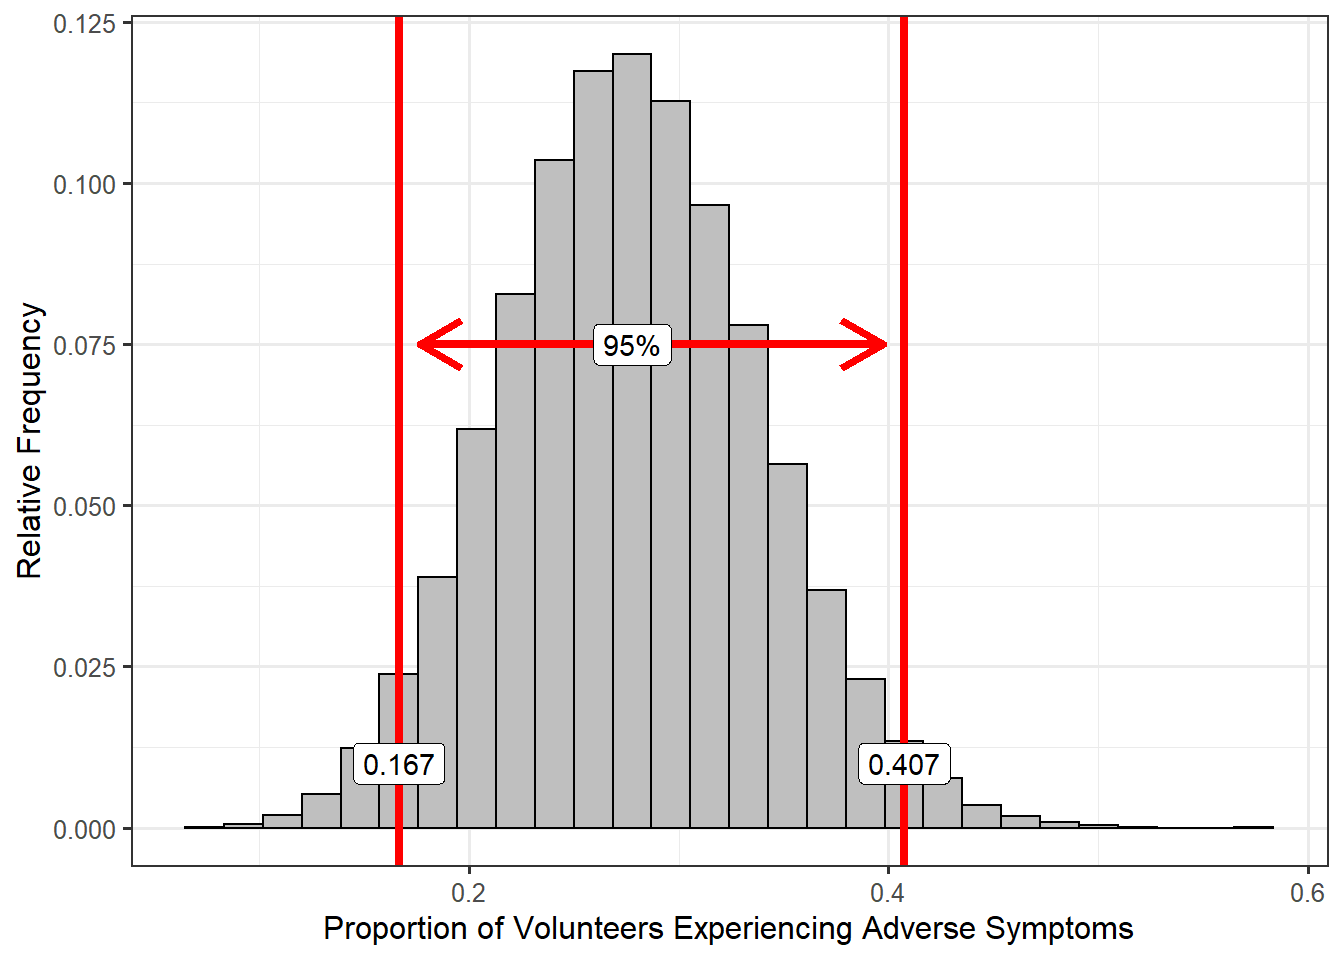
\includegraphics[width=0.8\linewidth]{./Images/samplingdistns-deepwater-ci-1} 

}

\caption{Construction of a confidence interval via bootstrapping for the proportion of volunteers assigned to wildlife who will develop adverse symptoms based on a sample of 54 volunteers.}\label{fig:samplingdistns-deepwater-ci}
\end{figure}

\BeginKnitrBlock{rmdtip}
The following is a general procedure for constructing confidence
intervals:

\begin{enumerate}
\def\labelenumi{\arabic{enumi}.}
\tightlist
\item
  Choose a confidence level \(k\).
\item
  Construct a model for the sampling distribution of the statistic.
\item
  Grab the middle \(k\)\% of values from the model in step (2).
\end{enumerate}

Notice that the definition of a confidence interval, and this general
procedure, apply regardless of the technique used for constructing the
model of the sampling distribution.
\EndKnitrBlock{rmdtip}

Confidence intervals are often misinterpreted; this comes from their
dependence on repeated sampling. When thinking about confidence
intervals, think about playing a game of ring toss: you toss a ring in
hopes of landing on top of a target. The target is the parameter
characterizing the population. The confidence interval is like a ring.
Since the confidence interval is constructed from a model of the
sampling distribution, it changes with each sample; that is, the
confidence interval itself is a statistic. Just like in ring toss where
the ring moves with each toss, the confidence interval moves with each
sample. However, the target stays fixed. Because of this, the following
interpretations are \emph{incorrect}:

\begin{itemize}
\tightlist
\item
  There is a 95\% chance that the proportion of volunteers assigned to
  clean wildlife who will experience adverse symptoms is between 0.167
  and 0.407.
\item
  95\% of volunteers assigned to clean wildlife in our sample (or
  population) had a value between 0.167 and 0.407.
\end{itemize}

The first statement is incorrect because it treats the parameter as the
thing that is moving. Once the data has been collected, the confidence
interval is a fixed quantity. At this point, neither the estimate nor
the parameter is moving; so, there is no probability left (it either
captured the parameter or it did not). Again, think about tossing a
ring; once the ring is tossed, you either captured the target or you did
not. There is no ``I captured the target with 95\% probability.''

The second statement is absurd in this case. A volunteer either had
respiratory symptoms or they did not; so, saying they had a value
between 0.167 and 0.407 is ridiculous. However, this is a common
misconception with confidence intervals. They are describing reasonable
values of the parameter as opposed to values of the variable in the
sample or population. We recommend sticking to interpreting a confidence
interval as specifying reasonable values for the parameter.

\BeginKnitrBlock{rmdtip}
Confidence intervals \emph{do not} provide a probability that the
parameter is inside. Nor do they tell you anything about the individual
values in a sample or population. They describe reasonable values of the
parameter.
\EndKnitrBlock{rmdtip}

\BeginKnitrBlock{rmdkeyidea}
Confidence intervals specify \emph{reaonable} values of the parameter
based on the data observed.
\EndKnitrBlock{rmdkeyidea}

This is a difficult concept to wrap our heads around; it seems natural
to associate the percentage with the values we have obtained. However,
our confidence is in the \emph{process}, not the resulting interval
itself. That is, 95\% confidence intervals work 95\% of the time;
however, this statement is about the process of constructing confidence
intervals. Once we have computed a convidence interval, it has either
worked or not; the problem is of course, that since we do not know the
parameter, we will never know if it worked or not. For this reason, we
prefer the interpretation of a confidence interval which avoids these
subtleties: a confidence interval specifies the reasonable values of the
parameter. The percentage (95\% vs 99\% for example) then just specifies
what we mean by ``reasonable.''

It may seem like a good idea to make a 100\% confidence interval to be
sure we always capture the parameter. But, such intervals are not
helpful in practice. For example, a 100\% confidence interval for the
proportion of volunteers experiencing adverse symptoms would be (0, 1).
But, this is useless; it essentially says that the proportion has to be
a number between 0 and 1, but we already knew that. Therefore, we must
balance the confidence we desire with the amount of information the
interval conveys.

\BeginKnitrBlock{rmdtip}
If you want both a high level of confidence but also a narrow interval,
increase the sample size. As the sample size increases, the variability
in the statistic decreases leading to a narrower interval.
\EndKnitrBlock{rmdtip}

\BeginKnitrBlock{rmdtip}
95\% confidence intervals are the most common in practice; however,
90\%, 98\%, and 99\% intervals are also used. It is extremely rare to
use less than a 90\% CI.
\EndKnitrBlock{rmdtip}

\section{Bringing it All Together}\label{bringing-it-all-together}

Consider the following question:

\begin{quote}
Is there evidence that more than 1 in 5 volunteers assigned to clean
wildlife will develop adverse respiratory symptoms?
\end{quote}

Let's answer this question using a confidence interval. Based on the
data obtained, we found that the 95\% confidence interval (CI) for the
proportion of volunteers experiencing adverse symptoms to be (0.167,
0.407). Is this data consistent with more than 1 in 5 volunteers
developing adverse symptoms? Yes, since there are proportions within
this interval which are larger than 0.2. But, \emph{consistency} is not
the same as \emph{evidence}; remember, evidence is the idea of ``beyond
a reasonable doubt.'' After all, is this data \emph{consistent} with
less than 1 in 5 volunteers developing adverse symptoms? Yes, since
there are proportions within this interval which are less than 0.2.

Confidence intervals specify reasonable values --- those values of the
parameter which are consistent with the data. This data is then
consistent with proportions that are both less than 0.2 and greater than
0.2. So, what can we say then? We can say that there is \emph{not
evidence} that more than 1 in 5 volunteers assigned to clean wildlife
will develop adverse respiratory symptoms, but the data \emph{is
consistent} with this claim.

We can say that there \emph{is evidence} that the proportion of
volunteers who develop symptoms is less than 0.5; there is evidence the
proportion of volunteers who develop symptoms is larger than 0.1. That
is, the data provides evidence that more than 10\% of volunteers develop
adverse symptoms and evidence that this percentage is not larger than
50\%. How do we know? Because values less than 10\% are not reasonble
values of the parameter based on the 95\% CI. Values like 0.1 are
outside of the confidence interval and are therefore not reasonable.
Similarly, values above 0.5 are outside the confidence interval and are
therefore not reasonable.

The power of a model for the sampling distribution is that it allows us
to determine which values of a parameter are reasonable and which values
are not.

\chapter{Quantifying the Evidence (Rejecting Bad
Models)}\label{NullDistns}

Again, the goal of statistical inference is to use the sample as a
snapshot of the underlying population (Figure
\ref{fig:nulldistns-statistical-process}). Recall that there are
essentially two categories of questions we ask when trying to perform
inference:

\begin{itemize}
\tightlist
\item
  Estimation: for example, what \emph{proportion} of volunteers who
  clean wildlife following an oil spill experience adverse respiratory
  symptoms?
\item
  Model Consistency: for example, is it reasonable that no more than 1
  in 5 volunteers who clean wildlife following an oil spill experience
  adverse respiratory symptoms?
\end{itemize}

\begin{figure}

{\centering 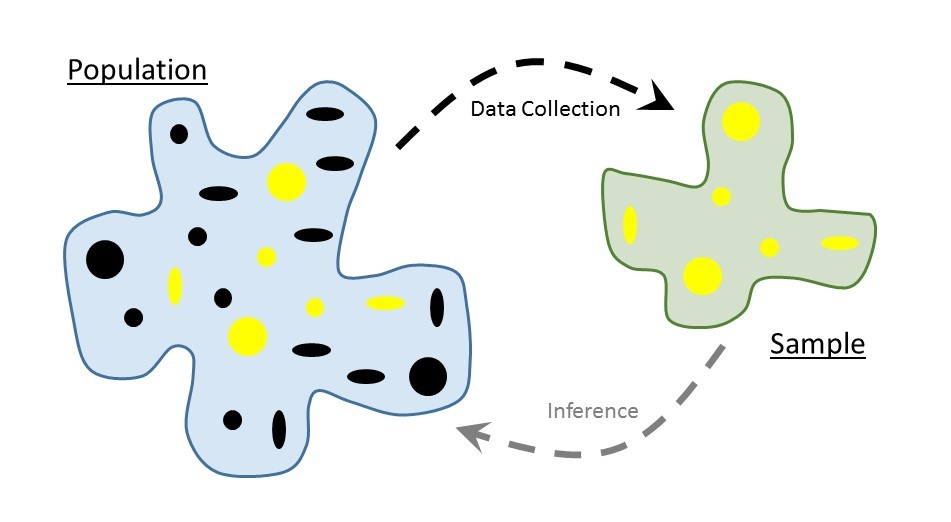
\includegraphics[width=0.8\linewidth]{images/Basics-Stat-Process} 

}

\caption{Illustration of the statistical process (reprinted from Chapter 1).}\label{fig:nulldistns-statistical-process}
\end{figure}

In the previous chapter we addressed these questions through the use of
confidence intervals --- by specifying reasonable values of the
parameters through a model of the sampling distribution. However, when
working with questions of the second type (model consistency), there is
a second approach; this latter approach is useful when confidence
intervals cannot be constructed for the particular question of interest
(see Unit 3).

Remember, assessing model consistency is similar to performing a trial
in a court of law. After gathering the evidence, the jury is left with
the following decision:

\begin{itemize}
\tightlist
\item
  Assuming the defendant is innocent, if the evidence is unlikely to
  have occurred (so the evidence is not consistent with innocence), then
  they vote ``guilty.''
\item
  Assuming the defendant is innocent, if the evidence is reasonably
  likely to have occurred (so the evidence is consistent with
  innocence), then they vote ``not guilty.''
\end{itemize}

The goal in this section is to somehow quantify the evidence against a
particular model to determine if we can say that the data is not
consistent with the given model.

\section{Some Subtleties}\label{some-subtleties}

In a U.S. trial, there are some subtleties that we should be aware of,
as they also creep up in statistical analyses and have implications for
how we interpret statistical results. First, the jury weighs the
evidence \emph{under the assumption of innocence}. That is, they first
develop a working hypothesis (the defendant is innocent). Then, the
likelihood of the evidence \emph{under this assumption} is determined.
For example, if a defendant were innocent of murder, it is unlikely to
have five eye witnesses stating the defendant was seen standing over the
victim, holding the murder weapon, and screaming ``I killed him!'' Since
that evidence does not jive with innocence, the jury convicts. If,
however, the only evidence is that five eye witnesses place the
defendant in the same city as the victim and the defendant matches the
description of someone seen fleeing the crime scene, then the jury would
not convict. Why? Because the evidence, while pointing toward guilt, is
not overwhelming; these things could have happened by chance alone.
Therefore, the evidence, while consistent with guilt does not provide
evidence for guilt.

As in the previous chapter, we are making a distinction between
``evidence for'' a hypothesis and the data being ``consistent with'' a
hypothesis. Evidence for a particular claim is only established by
providing evidence against the opposite statement. However, consistency
can be established without disqualifying any other statement; that is,
data can be consistent with two opposing claims, but data cannot provide
evidence for two opposing claims.

Also notice that a jury saying ``not guilty'' is not the same as saying
``innocent.'' That is, a lack of evidence to convict does not imply the
defendant is innocent. A lack of evidence is simply a lack of evidence.
The defendant may still be guilty, but the evidence has just not proven
it.

Similarly, when assessing model consistency, we will weigh the data
\emph{under the null hypothesis} (our working assumption). Then, the
likelihood of our data occurring by chance alone \emph{under this
hypothesis} is determined. If that likelihood is small (data is not
consistent with the null hypothesis), we can conclude the data supports
the alternative hypothesis (guilty). If, however, that likelihood is
large (data is consistent with the null hypothesis), we can only
conclude that the data is consistent with the hypotheses. We are
\emph{not} able to say ``supports the null'' because that would be like
saying a defendant is innocent. We can't prove innocence because we
started by assuming it!

\section{Assuming the Null
Hypothesis}\label{assuming-the-null-hypothesis}

Consider the question we have been asking regarding the
\protect\hyperlink{CaseDeepwater}{Deepwater Horizon Case Study}:

\begin{quote}
Is there evidence that more than 1 in 5 volunteers assigned to clean
wildlife develop adverse respiratory conditions?
\end{quote}

Remember, we framed this question through statements about a parameter
in Chapter \ref{Questions}:

\begin{quote}
\(H_0:\) the proportion of volunteers assigned to clean wildlife who
develop adverse respiratory symptoms is no more than 0.20.\\
\(H_1:\) the proportion of volunteers assigned to clean wildlife who
develop adverse respiratory symptoms exceeds 0.20.
\end{quote}

Within the sample we observed that 27.8\% of volunteers experienced
adverse symptoms, which is certainly more than the 0.20; therefore, the
data is at least trending toward the alternative hypothesis. However, it
is also possible that we just have a strange sample; that is, it is
possible our data is a fluke, resulting in an estimate larger than 0.2
by chance alone. As we discussed in the previous chapter, we expect our
estimate to vary to some degree from one sample to another. Essentially,
we need to know if 27.8\% of volunteers experiencing symptoms is a
strong signal that the rate within the popoulation is larger than 0.2 (1
in 5) or whether 27.8\% is simply a fluke that might happen due to
sampling variability. While we are going to be attacking the question
differently in this chapter than the previous, we see that the key is
still variability in the estimate. That is, we are back to the
\emph{Fourth Fundamental Idea of Inference}. As stated above, in order
to determine evidence for one statement (captured by the alternative
hypothesis), we begin by assuming the opposite statement (captured by
the null hypothesis) as our working assumption. That is, if we want to
know if 27.8\% of volunteers experiencing adverse symptoms is
``evidence,'' we need to figure out what we \emph{expect} to happen
\emph{if only 1 in 5 volunteers actually develop adverse respiratory
symptoms} (the statement represented by the equality portion of the null
hypothesis).

Consider this last statement. It is equivalent to saying ``what type of
evidence would we expect for an innocent person?'' Only when we know
what to expect can we determine if the evidence in front of us is
extreme enough to convict. Only when we know what to expect can we
determine if the observed sample provides evidence in favor of the
alternative. So, we enter a fake world\ldots{}a world in which exactly 1
in 5 volunteers actually develop respiratory symptoms. That is, we enter
a world in which the null hypothesis is true. Now, in this world, how do
we know what to expect? We construct the sampling distribution for the
proportion under this assumption that the null hypothesis is true; this
is known as the \textbf{null distribution}.

\BeginKnitrBlock{definition}[Null Distribution]
\protect\hypertarget{def:defn-null-distribution}{}{\label{def:defn-null-distribution}
\iffalse (Null Distribution) \fi{} }The sampling distribution of a
statistic \emph{if} the null hypothesis is true.
\EndKnitrBlock{definition}

The null distribution, the last in our \emph{Distributional Quartet}, is
a sampling distribution; it is just a sampling distribution in a world
in which the null hypothesis is true. As a result, the process for
constructing the null distribution is very similar to the process for
constructing the sampling distribution (illustrated in Figure
\ref{fig:nulldistns-null-distribution}:

\begin{enumerate}
\def\labelenumi{\arabic{enumi}.}
\tightlist
\item
  Sample randomly from a fake population where the null hypothesis is
  true.
\item
  For each sample, compute the statistic of interest.
\item
  Repeat steps 1 and 2 several thousand times.
\item
  Plot the statistics retained from each sample.
\end{enumerate}

\begin{figure}

{\centering 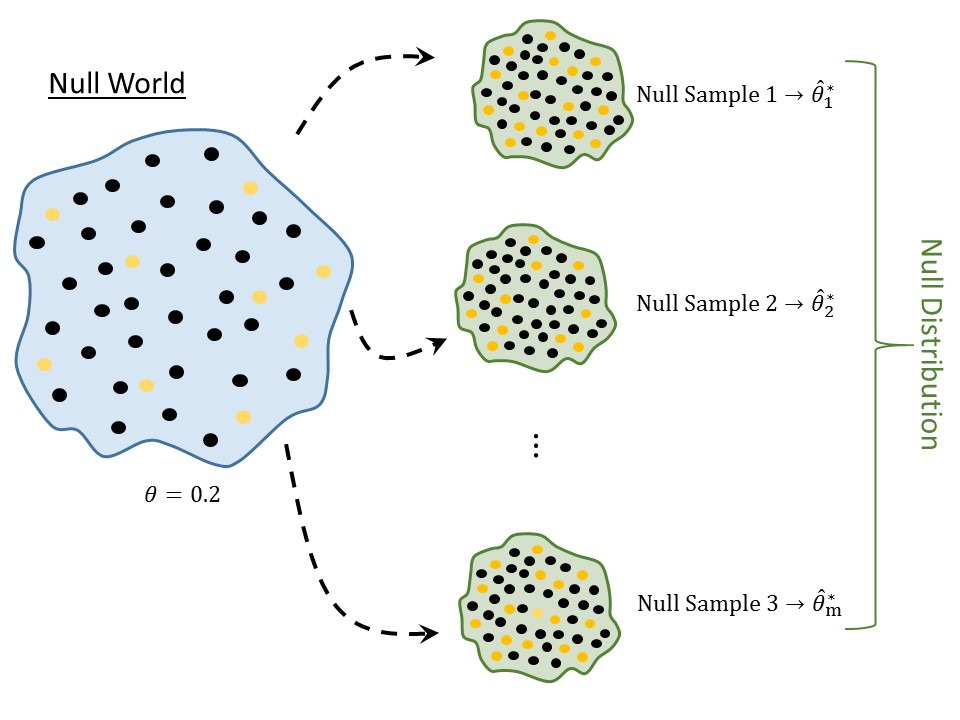
\includegraphics[width=0.8\linewidth]{./images/NullDistns-Null-Distribution} 

}

\caption{Illustration of constructing a null distribution.  Notice the similarity to constructing the sampling distributon.}\label{fig:nulldistns-null-distribution}
\end{figure}

Notice that these are the same steps as in constructing a sampling
distribution with the exception that instead of sampling from the
population of interest, we sample from a hypothetical population in
which the null distribution is true.

Since the null distribution is a sampling distribution when a particular
hypothesis is true, we are constrained by the same limitations as
before. Namely, we are unable to construct the actual the null
distribution; instead, we must construct a model for it. More, since the
null distribution is a sampling distribution, the same techniques we use
for modeling the sampling distribution can be modified to model the null
distribution. The key is to enforce the null hypothesis to be true. As
with sampling distributions, we will emphasize the empirical model
approach.

Using the computer, we first create a virtual world in which the null
hypothesis is true. This often involves adjusting the original sample in
order to make it consistent with having been drawn from a population in
which the null hypothesis were true. The augmented data becomes the null
world. We are then able to bootstrap from the augmented data to simulate
what would happen if the null hypothesis were true. The details of this
procedure are beyond the scope of our current discussion; it is more
important to understand the conceptual idea of a null distribution at
this point.

Figure \ref{fig:nulldistns-deepwater-null} represents a model for the
null distribution of the proportion of volunteers in a sample of 54
assigned to clean wildlife which would develop adverse sympoms when the
null hypothesis is that the proportion is 0.20.

\BeginKnitrBlock{rmdtip}
A null distribution is tied to a specific null hypothesis. A sampling
distribution does not require a hypothesis to construct. So, while a
sampling distribution could be used to address a variety of null
hypotheses, a null distribution can only be used to address the
corresponding set of hypotheses for which it was developed.
\EndKnitrBlock{rmdtip}

\begin{figure}

{\centering 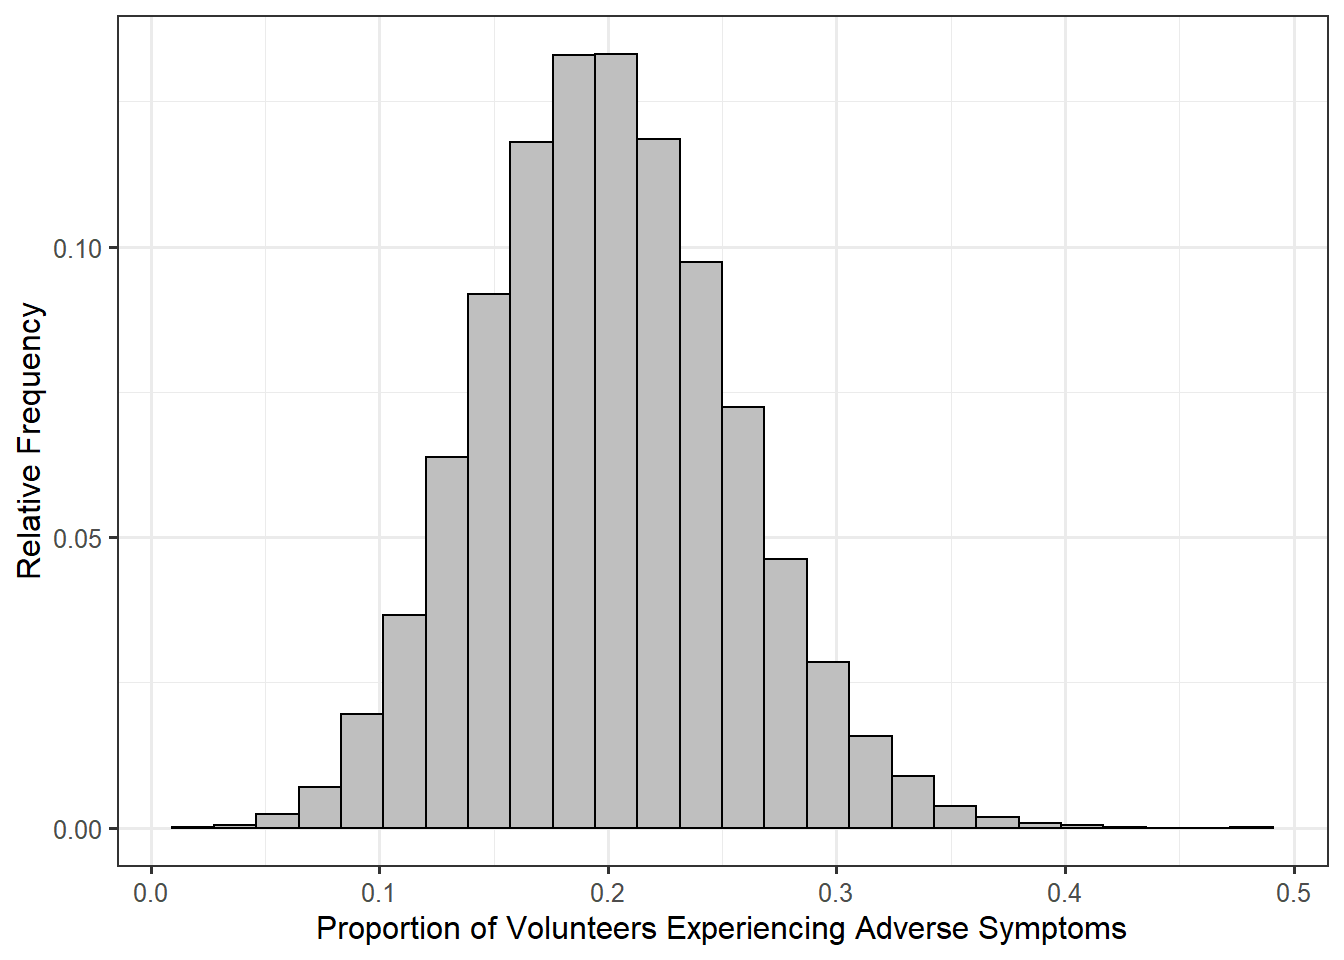
\includegraphics[width=0.8\linewidth]{./Images/nulldistns-deepwater-null-1} 

}

\caption{Null distribution for the proportion of volunteers assigned to clean wildlife experiencing adverse respiratory symptoms.  Null hypothesis is that the proportion is 0.20; this is based on a sample of size 54.}\label{fig:nulldistns-deepwater-null}
\end{figure}

As we are introducing the concept of a null distribution, we will stick
to modeling the null distribution of a statistic. Often times in a
statistical analysis, the null distribution is computed for a numerical
quantity known as a standardized statistic. These will be discussed more
in later units of the text.

\section{Using the Null Distribution}\label{using-the-null-distribution}

From the figure, we see that \emph{if the null hypothesis were true} ---
if only 1 in 5 volunteers assigned to clean wildlife experienced
symptoms --- then in a sample of 54 individuals, we would expect the
proportion who experienced symptoms to be somewhere between 0.1 and 0.3.
\emph{If the null hypothesis were true}, it would be nearly impossible
that half of the individuals experienced symptoms (since 0.5 is way off
in the tail of the distribution). The further in the tail region, the
more extreme the sample. The question is then how extreme is our sample?
Again, the null distribution is just setting up expectations; now, we
have to weigh the data against those expectations.

In our sample, we observed 27.8\% of volunteers who experienced
symptoms. Since 0.278 is towards the center of the distribution, we
would say that it is not an extreme sample. In order to quantify how
extreme (or not extreme) it is, we compute the fraction of values which
are more extreme (larger in this case) than the value observed; that is,
we compute the fraction of values that appear further in the right than
0.278 in the null distribution. Figure
\ref{fig:nulldistns-deepwater-pvalue} illustrates this computation.
Based on the null distribution, there is a 10.6\% chance that \emph{if
the null hypothesis were true} --- only 1 in 5 volunteers actually
experienced symptoms --- that in a random sample of 54 volunteers we
would obtain data this extreme or more so by chance alone. Essentially,
this tail area is quantifying the strength of the evidence. The smaller
this area, the further in the tail region our data is; that is, the
smaller this area, the more unexpected our data. Therefore, small areas
indicate that the data (our evidence) does not jive with our
expectations under the null (innocence), forcing us to conclude the data
provides evidence \emph{against} the null hypothesis (guilty verdict).
In our case, since the area is relatively large, our data is consistent
with what we might expect if the null were true. Therefore, in this
case, we conclude that there is no evidence that the rate of those
experiencing symptoms exceeds 1 in 5. This area is known as the
\textbf{p-value}.

\begin{figure}

{\centering 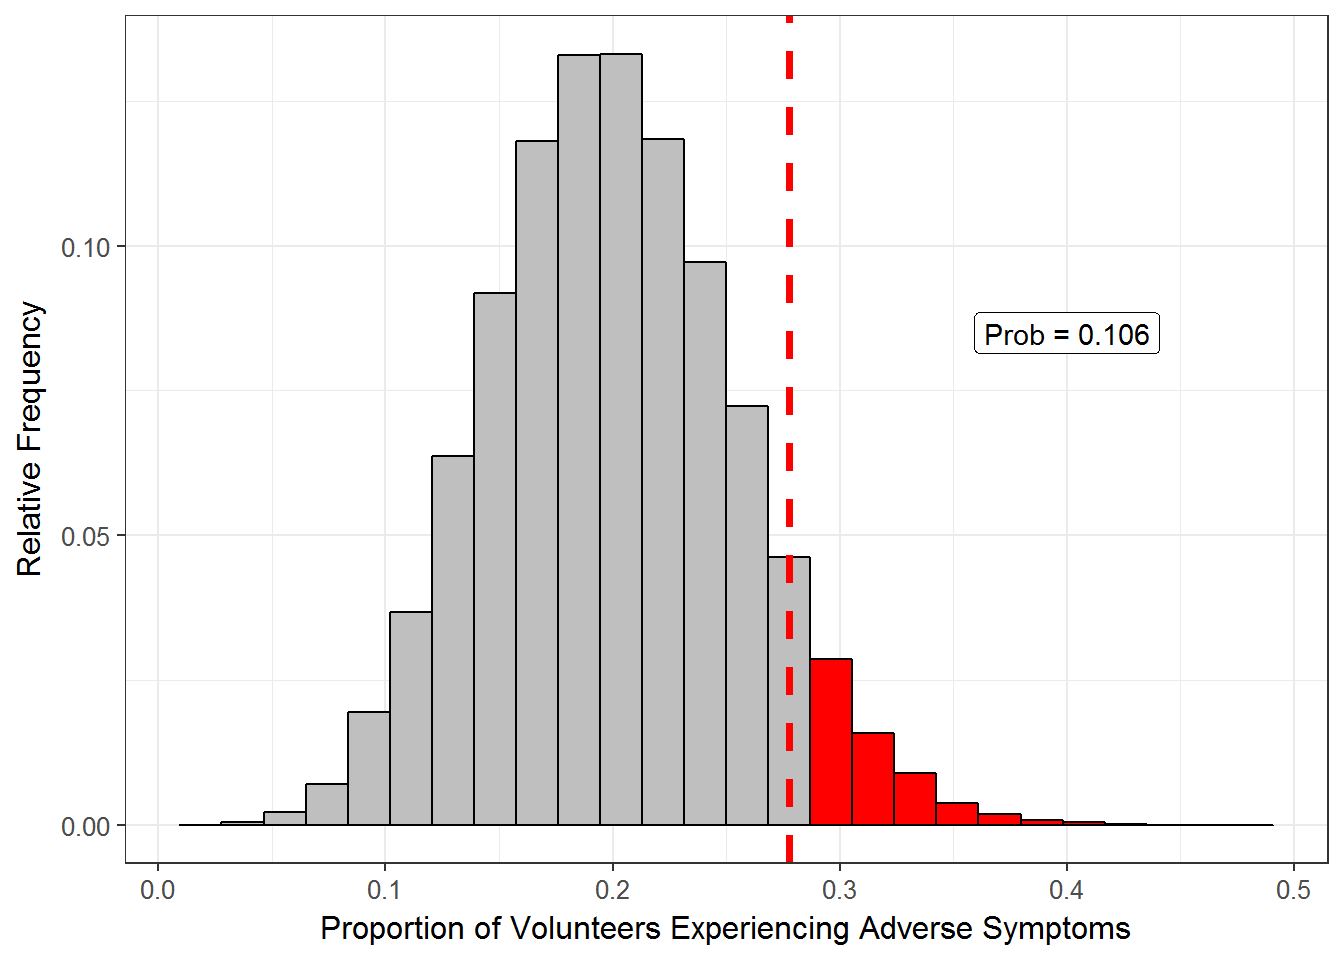
\includegraphics[width=0.8\linewidth]{./Images/nulldistns-deepwater-pvalue-1} 

}

\caption{Likelihood of obtaining a sample as extreme or more so as that of the original sample when the parameter of interest is the proportion of volunteers assigned to clean wildlife experiencing adverse respiratory symptoms.  Null hypothesis is that the proportion is 0.20; this is based on a sample of size 54.}\label{fig:nulldistns-deepwater-pvalue}
\end{figure}

\BeginKnitrBlock{definition}[P-Value]
\protect\hypertarget{def:defn-pvalue}{}{\label{def:defn-pvalue}
\iffalse (P-Value) \fi{} }The probability, assuming the null hypothesis
is true, that we would observe a statistic, from sampling variability
alone, as extreme or more so as that observed in our sample. This
quantifies the strength of evidence against the null hypothesis. Smaller
values indicate stronger evidence.
\EndKnitrBlock{definition}

It is natural to ask ``how small does the p-value need to be to prove a
statement?'' Like a trial, the weight of the evidence presented depends
on the context. In some studies, a p-value less than 0.01 may be strong
evidence while in other studies a p-value less than \(10^{-6}\) is
required. And, as in a trial, it is not only the strength of the
evidence but the type of evidence presented (DNA evidence may be
stronger than fingerprint evidence). In statistics, it is important to
consider the \emph{effect size} (some measure of the signal in the data)
as well as the p-value. That is, consider whether the difference between
the estimate and the null value is actually large; this is always based
on subject-matter expertise. It is often helpful to report a confidence
interval alongside a p-value.

\BeginKnitrBlock{rmdtip}
While what constitutes ``significant'' may vary from discipline to
discipline, the list below is a good rule of thumb:

\begin{itemize}
\tightlist
\item
  \(p \geq 0.1\): no evidence against the null hypothesis.
\item
  \(0.05 \leq p < 0.1\): weak evidence against the null hypothesis.
\item
  \(0.01 \leq p < 0.05\): some evidence against the null hypothesis.
\item
  \(0.001 \leq p < 0.01\): evidence against the null hypothesis.
\item
  \(p < 0.001\): strong evidence against the null hypothesis.
\end{itemize}

As with any rule of thumb, this should not be considered binding and may
vary depending on the application.
\EndKnitrBlock{rmdtip}

\BeginKnitrBlock{rmdtip}
A p-value should never be reported in isolation. It should always be
accompanied by a confidence interval, a numerical summary of the data,
or a graphical summary of the data --- something which indicates the
effect size and variability in the data.
\EndKnitrBlock{rmdtip}

\BeginKnitrBlock{rmdtip}
The following is a general procedure for computing a p-value:

\begin{enumerate}
\def\labelenumi{\arabic{enumi}.}
\tightlist
\item
  Define the null and alternative hypotheses.
\item
  Construct a model for the null distribution of the desired statistic.
\item
  Compute the desired statistic for the original sample.
\item
  Overlay the statistic from step (3) on the model developed in step
  (2), and then compute the area under the curve for values \emph{more
  extreme} than that observed in step (3).
\end{enumerate}

Notice that the definition of a p-value, and this general procedure,
apply regardless of the technique used for constructing the model of the
null distribution.
\EndKnitrBlock{rmdtip}

Like confidence intervals, p-values are often misinterpreted. In fact,
they have become so abused that some researchers argue against their
use. It is our opinion that the p-value can be a useful tool once it is
appropriately understood; so, let's dispell some of the misconceptions.
Consider these \emph{incorrect} statements regarding the p-value
obtained for the \protect\hyperlink{CaseDeepwater}{Deewater Horizon Case
Study} computed above:

\begin{itemize}
\tightlist
\item
  There is a 10.6\% chance that only 1 in 5 volunteers assigned to clean
  wildlife will experience adverse symptoms.
\item
  Since the p-value is large, there is evidence (or the data supports
  the claim) that 1 in 5 volunteers assigned to clean wildlife will
  experience adverse symptoms.
\end{itemize}

The first statement incorrectly assumes that there is some chance that
the null hypothesis is true. Remember, our two hypotheses are statements
about the parameter. One is true and other is not. Our ignorance does
not change this; therefore, it does not make sense to talk about the
probability of the null being true or false. Instead, our job is to
quantify the likelihood of the data \emph{assuming the null is true}.
The p-value is about the likelihood of the data under a particular model
(the null hypothesis).

The second statement makes the common mistake that a lack of evidence
for the alternative is evidence in favor of the null. A lack of evidence
is like a ``not guilty'' verdict. It simply means we were not convinced.
However, it does not mean that the defendant is innocent. All we are
saying with the large p-value in this case is that the data is
\emph{consistent} with only 1 in 5 volunteers getting adverse symptoms;
unfortunately, it is also \emph{consistent} with more than 1 in 5
volunteers getting adverse symptoms. This may be an unsatisfying
conclusion, but it is still a conclusion nonetheless. Our conclusion is
based on assessing the variability of a the statistic under a particular
model. This is captured in our last of the \emph{Five Fundamental Ideas
of Inference}:

\BeginKnitrBlock{rmdfivefund}
\textbf{Fundamental Idea V}: With a model for the distribution of a
statistic under a proposed model, we can quantify the the likelihood of
an observed sample under that proposed model. This allows us to draw
conclusions about the corresponding parameter, and therefore the
population, of interest.
\EndKnitrBlock{rmdfivefund}

\section{Sampling Distributions vs.~Null
Distributions}\label{sampling-distributions-vs.null-distributions}

Clearly the sampling distribution and null distribution of a statistic
are closely related. The difference is that the null distribution is
created under a proposed model while the sampling distribution lets the
data speak for itself. It is worth taking just a moment to highlight the
differences in the use of these two components of the
\emph{Distributional Quartet}.

The sampling distribution is centered on the true value of the
parameter; the null distribution is centered on the null value. Once we
assume the null hypothesis is true, we have a value for the parameter;
as a result, we expect the sampling distribution under this assumption
(that is, the null distribution) to be centered on this hypothesized
value. So, null distributions are \emph{always} centered on the null
value.

Sampling distributions lead to confidence intervals by specifying
reasonable values of the parameter.

Null distributions lead to p-values by quantifying the likelihood of our
data under a proposed model.

\BeginKnitrBlock{rmdtip}
Model the sampling distribution to construct a confidence interval; to
assess a hypothesis the null value is overlayed on the sampling
distribution. Extreme values of the distribution are unreasonable values
for the parameter.

Model the null distribution to compute a p-value; to assess a
hypothesis, the statistic from the sample is overlayed on the null
distribution. Extreme values of the distribution are values which
provide evidence against the null hypothesis.
\EndKnitrBlock{rmdtip}

\chapter{Using the Tools Together}\label{RecapLanguage}

In this unit, we have introduced the key components in both the language
and logic of statistical inference. In fact, with a firm grasp of the
concepts in this unit, you should be able to read and interpret key
statistical findings. All statistical analyses make use of the
\emph{Five Fundamental Ideas of Inference} and alternate between the
members of the \emph{Distributional Quartet}. The context of each
problem differs, but the logic remains the same. In this chapter, we
present another analysis based on the
\protect\hyperlink{CaseDeepwater}{Deepwater Horizon Case Study},
annotating it along the way to see how these elements work together
fluidly to reach a conclusion. Specifically, we are interested in the
following question:

\begin{quote}
Are volunteers assigned to clean wildlife at higher risk of developing
adverse respiratory symptoms compared to those volunteers who do not
come into direct contact with oil? If so, estimate the increased risk.
\end{quote}

\section{Framing the Question (Fundamental Idea
I)}\label{framing-the-question-fundamental-idea-i}

We are really interested in whether the rate of respiratory symptoms in
one group of volunteers is larger than that in a second group.
Therefore, our working assumption is that the rate of respiratory
symptoms for those assigned to clean wildlife is no more than that for
those assigned to tasks which do not involve direct exposure to oil.
That is, we have

\begin{quote}
\(H_0:\) the rate of adverse respiratory symptoms for volunteers
assigned to clean wildlife is no greater than that for those assigned to
tasks which do not involve direct exposure to oil.\\
\(H_1:\) the rate of adverse respiratory symptoms is greater for
volunteers assigned to clean wildlife compared to those assigned to
tasks which do not involve direct exposure to oil.
\end{quote}

We can also state this more formally with mathematical notation as
follows:

\begin{quote}
Let \(\theta_1\) be the rate of developing adverse respiratory symptoms
for volunteers assigned to clean wildlife.\\
Let \(\theta_2\) be the rate of developing adverse respiratory symptoms
for volunteers assigned to tasks without direct exposure to oil.\\
\(H_0: \theta_1/\theta_2 \leq 1\)\\
\(H_1: \theta_1/\theta_2 > 1\)
\end{quote}

The ratio \(\theta_1/\theta_2\) is known as the \emph{relative risk} as
it captures the increased risk for one group compared to another.

Notice that this is a well-posed question as it centers on parameters
which characterize the population. Therefore, it can be answered with
appropriate data.

\begin{quote}
Distribution of the Population: Our questions of interest are about the
population and therefore focus on characterizing this distribution.
\end{quote}

\section{Getting Good Data (Fundamental Idea
II)}\label{getting-good-data-fundamental-idea-ii}

As we are working with previously collected data, we are unable to
design a good sampling scheme. The only thing we can do at this point is
critique the sample we have. The key question to ask ourselves is
whether there is any reason that this group of volunteers differs
systematically from other volunteers working oil spills. For example,
this oil spill occurred in the Gulf of Mexico; the majority of
volunteers were then naturally residents of Gulf states. It is possible
that these residents are somehow fundamentally different with respect to
their risk of developing adverse respiratory symptoms compared to the
remainder of the United States. If that is the case, the results of this
study would not generalize to oil spills occuring in the Atlantic.
However, it is probably reasonable to say that these results would apply
to future oil spills in the Gulf. If, on the other hand, we believe this
group of volunteers is representative of volunteers for other oil
spills, regardless of location, our results could generalize more
broadly.

Also note that this was not a controlled experiment. Volunteers were not
randomly allocated to their assignments that we know of. Therefore, our
results could be somewhat limited. The two groups should be compared
regarding other attributes (this data is unavailable to us currently) in
order to determine if they are similar with respect to other variables
which may potentially confound the results.

\section{Presenting the Data (Fundamental Idea
III)}\label{presenting-the-data-fundamental-idea-iii}

The heart of this question is comparing the rate of adverse events in
each group. Figure \ref{fig:recaplanguage-deepwater-plot} makes this
comparison.

\begin{figure}

{\centering 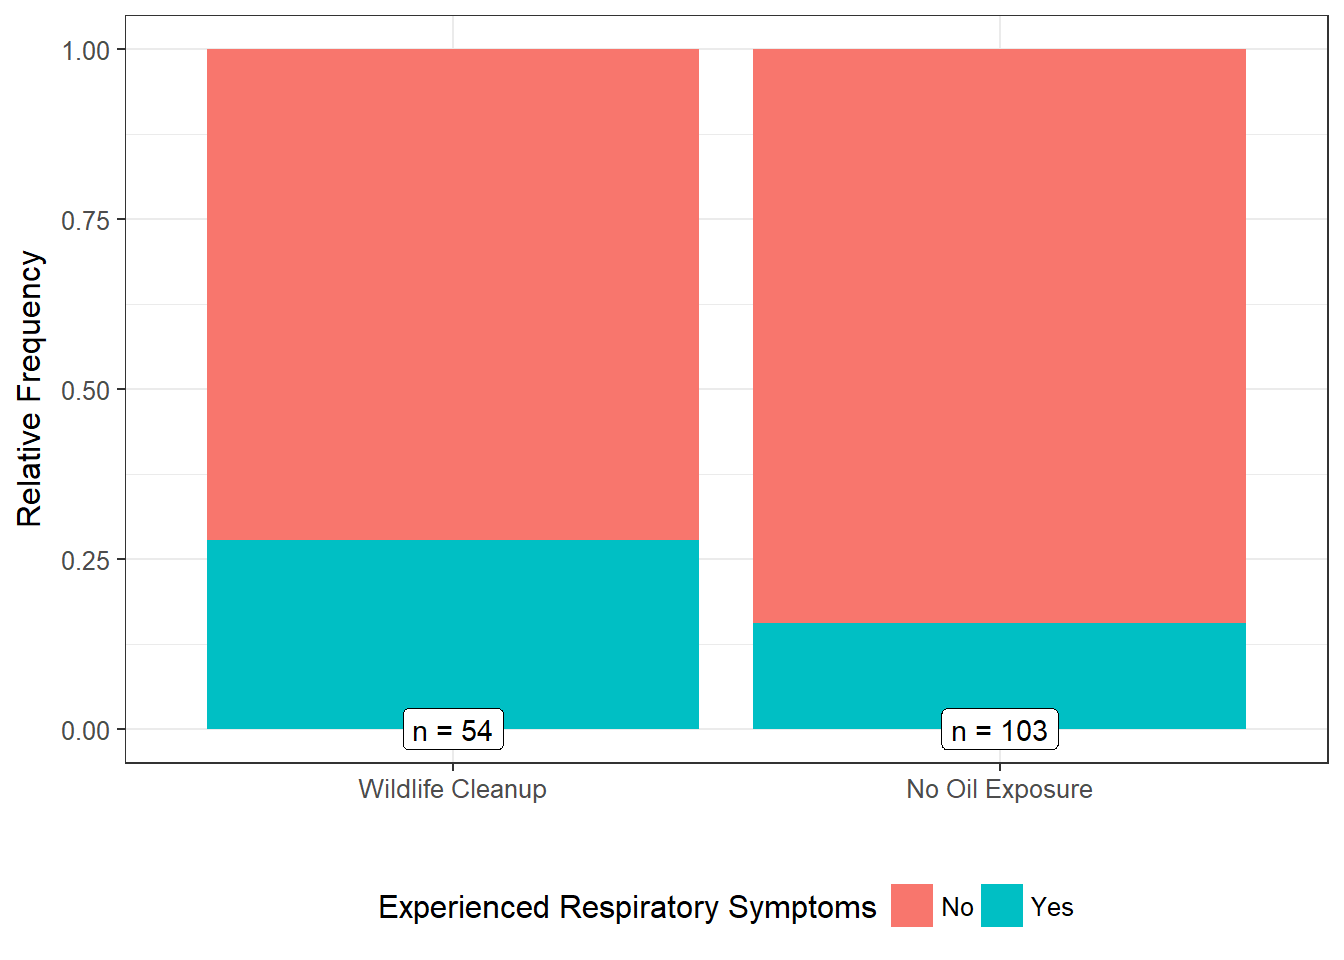
\includegraphics[width=0.8\linewidth]{./Images/recaplanguage-deepwater-plot-1} 

}

\caption{The risk of developing adverse respiratory symptoms for volunteers assigned to clean wildlife and those volunteers assigned to tasks which do not have direct exposure to oil.}\label{fig:recaplanguage-deepwater-plot}
\end{figure}

As seen in the figure, the rate of adverse respiratory symptoms is
larger in the group of volunteers assigned to wildlife cleanup. The rate
of respiratory symptoms is 1.79 times higher in the volunteers assigned
to clean wildlife compared to those assigned to tasks with no direct oil
exposure.

Notice that we reported the relative risk comparing the two groups as it
is directly tied to how we specified the hypotheses above. That is, the
statistic we report is governed by the parameter of interest; we compute
a value in the sample to estimate the corresponding value in the
population.

\begin{quote}
Distribution of the Sample: graphics and numerical summaries
characterize this distribution, informing us about the underlying
population. This is possible as long as the sample is representative of
the population.
\end{quote}

\section{Quantifying the Variability in the Estimate (Fundamental Idea
IV)}\label{quantifying-the-variability-in-the-estimate-fundamental-idea-iv}

While we have an estimate for the increased risk of adverse respiratory
symptoms for those volunteers assigned to clean wildlife, the estimate
has not taken into account the variability in the sample. In order to
quantify this variability, we use a bootstrap procedure to model the
sampling distribution of the risk ratio. Observe that we focus on the
sampling distribution of the statistic that estimates the parameter of
interest.

Recall that the bootstrap mimics the process for generating a sampling
distribution. In this case, ``repeating the study'' involves collecting
data from not one, but two groups. So, we must resample both from the 54
volunteers who were assigned to clean wildlife and the 103 volunteers
assigned to tasks not involving direct oil exposure. Each time we
resample, we ensure that we select 54 volunteers who clean wildlife and
103 who do not. We need the process of the original study to be
maintained. Each time we resample from these groups, we compute the
relative risk and retain this value. Figure
\ref{fig:recaplanguage-sampling-distribution} shows the sampling
distribution for the relative risk comparing these two groups. Again, it
is important to note that we are not generating \emph{new} data; we are
\emph{resampling}/\emph{reusing} the original sample.

\begin{figure}

{\centering 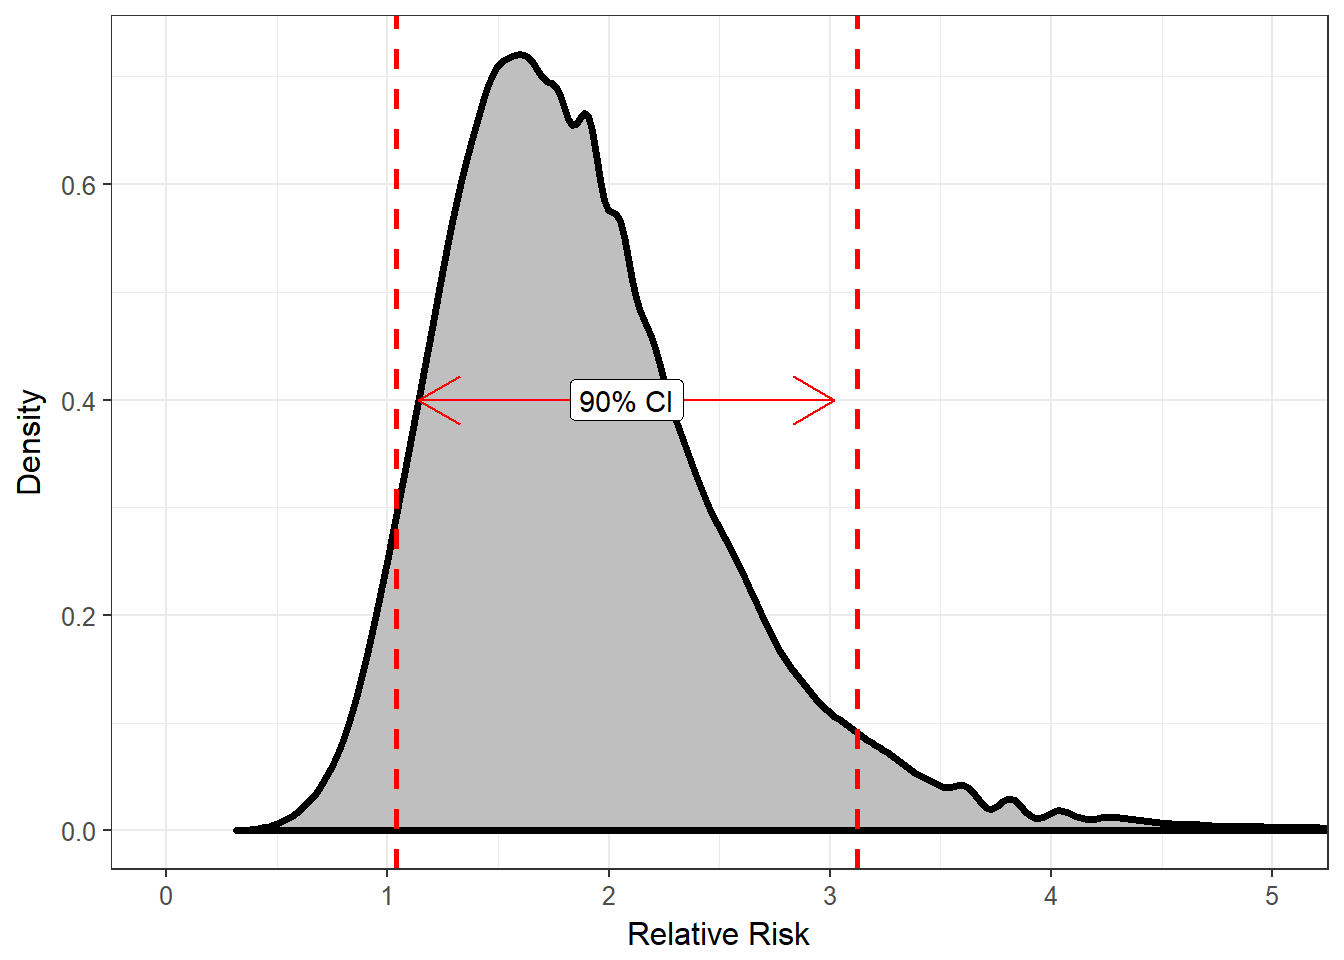
\includegraphics[width=0.8\linewidth]{./Images/recaplanguage-sampling-distribution-1} 

}

\caption{Model of the sampling distribution for the relative risk comparing volunteers assigned to clean wildlife to volunteers assigned to tasks not involving oil exposure.  The model was developed via bootstrapping using 50000 replications.}\label{fig:recaplanguage-sampling-distribution}
\end{figure}

Volunteers assigned to clean wildlife are 1.79 times (90\% CI = (1.04,
3.12)) more likely to experience adverse respiratory symptoms compared
to those volunteers assigned to tasks not requiring direct exposure to
oil. Our data is consistent with volunteers assigned to clean wildlife
being at increased risk compared to those who do not have direct
exposure to oil.

\begin{quote}
Sampling Distribution: allows us to quantify the variability in the
statistic and provide an interval estimate for the paraemter which
incorporates this variability.
\end{quote}

\section{Quantifying the Evidence (Fundamental Idea
V)}\label{quantifying-the-evidence-fundamental-idea-v}

In order to quantify the departure of the data from our working
assumption that the risk is for those assigned to clean wildlife is no
more than that for those assigned to tasks without direct oil exposure,
we rely on the null distribution and compute a p-value.

\begin{figure}

{\centering 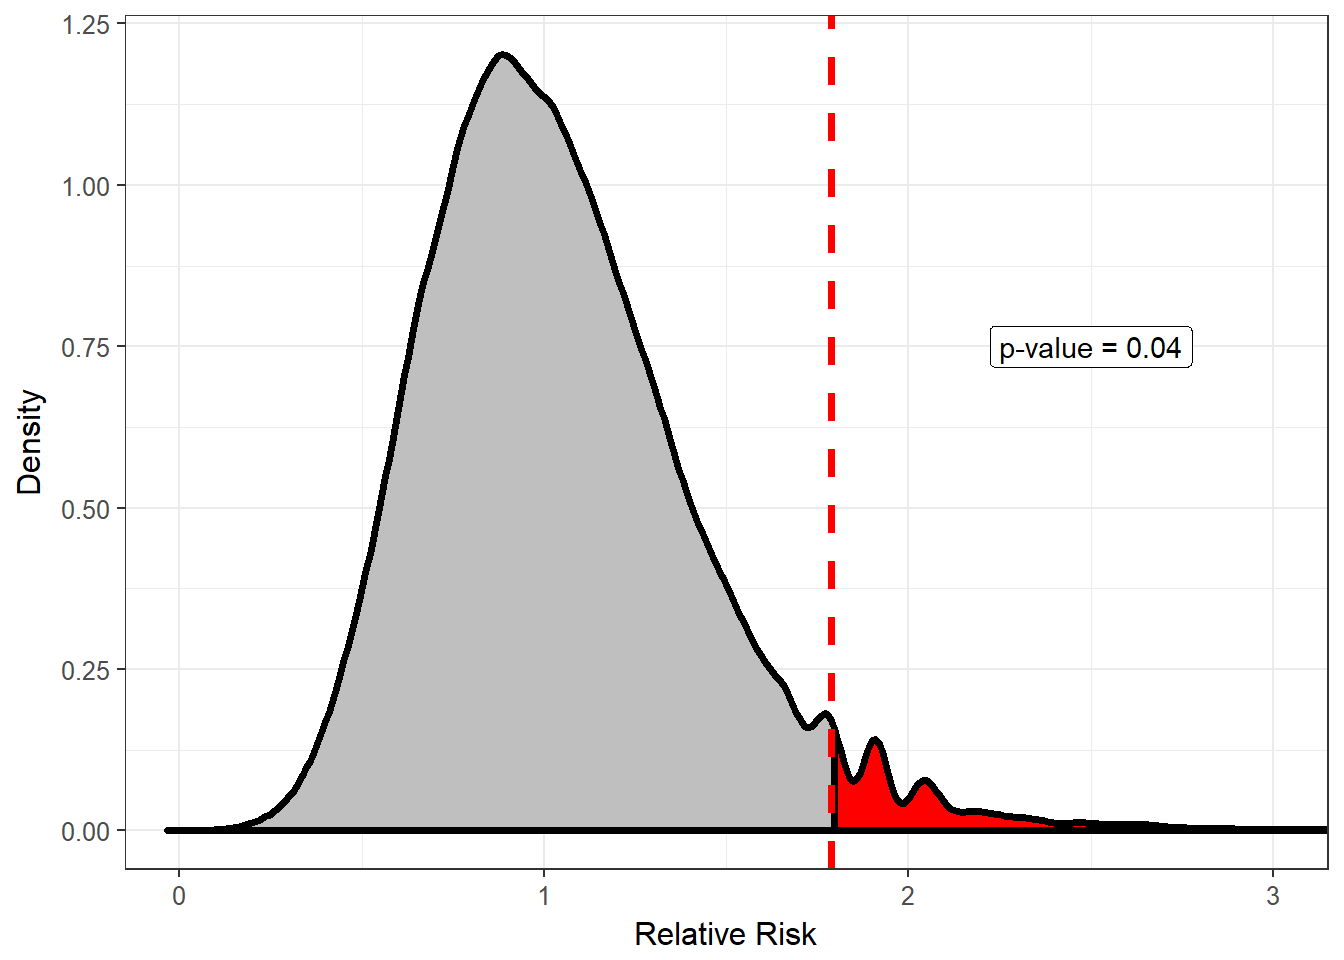
\includegraphics[width=0.8\linewidth]{./Images/recaplanguage-null-distribution-1} 

}

\caption{Null distribution for the relative risk comparing volunteers assigned to clean wildlife to volunteers assigned to tasks not involving oil exposure.  The null hypothesis assumed the two groups of volunteers had the same risk.  The null distribution was developed via bootstrapping using 50000 replications.}\label{fig:recaplanguage-null-distribution}
\end{figure}

There is some (borderline weak) evidence (p = 0.04) to suggest that
volunteers exposed to oil have an increased risk of developing adverse
respiratory symptoms. Given the estimated level of this increased risk,
we believe this is something health officials should investigate
further. It would be worth investigating what aspects of the oil
exposure may have led to the increased risk to determine if it can be
avoided in the future.

Note we are careful to not claim that the assignments have caused an
increase in the risk as this data is not from a controlled experiment.
This is one of the limitations of this analysis. However, if we are able
to assume the two groups are fairly similar with respect to other
attributes --- that is, there is no reason why people prone to
respiratory symptoms would become assigned to wildlife cleaning --- then
we may have some reason to believe the results are causal. We will
wrestle more with these types of conclusions in future units.

\begin{quote}
Null Distribution: allows us to quantify the level of evidence against a
particular claim; how strongly do the data disagree with the working
assumption.
\end{quote}

\section{Summary}\label{summary}

Notice that our analysis moved through the \emph{Five Fundamental
Ideas}, and in doing so made use or referenced each of the four
components of the \emph{Distributional Quartet}. As we move through the
remainder of the text, we will explore how these frameworks are used in
various other analysis scanarios. As we do, we reveal additional
concepts that underly statistical modeling.

We admit that there are several other questions that may be raised by
the above analysis. This unit is meant to introduce the big concepts of
inference. We will concern ourselves more with the details as we
progress through the text.

\part{Unit II: Implementing the Logic of Inference for a
Single
Mean}\label{part-unit-ii-implementing-the-logic-of-inference-for-a-single-mean}

\hypertarget{CaseBabies}{\chapter{Case Study: Birth Weights of
Babies}\label{CaseBabies}}

The Centers for Disease Control and Prevention (CDC) --- using data
provided by the U.S. Department of Health and Human Services, National
Center for Health Statistics, the Division of Vital Statistics and the
CDC --- maintains a database on all babies born in a given
year\footnote{\url{http://wonder.cdc.gov/natality-current.html}}. This
database contains key metrics on each child born, including the weight
of the infant. Low birthweight can be indicative of poor health or
illness in children. High birthweight can be indicative of obesity later
in life. One use of this database is for researchers to examine links
between lifestyle choices of the parents (such as whether the mother
consumed alcohol during pregnancy) and birthweight of the infant.

Chihara and Hesterberg (\protect\hyperlink{ref-Chihara2011}{2011})
describe a random sample from this database; specifically, the sample
consists of 1009 babies born in North Carolina during 2004. The babies
each had a gestation period of at least 37 weeks (full term) and were
single births (no twins, triplets, etc.). For each birth in the sample,
we have the following information:

\begin{itemize}
\tightlist
\item
  Age: Age of the mother (in years).
\item
  Tobacco: An indicator of whether the mother used tobacco during the
  pregnancy.
\item
  Alcohol: An indicator of whether the mother used alcohol during the
  pregnancy.
\item
  Sex: Sex of the child.
\item
  Weight: Weight of the child at birth (grams).
\item
  Gestation: Gestation time (length of pregnancy, weeks).
\item
  Smoker: An indicator of whether the mother is a current smoker.
\end{itemize}

A subset of the collected data is shown in Table
\ref{tab:casebabies-table}.

\begin{table}

\caption{\label{tab:casebabies-table}Subset of a sample of 1009 babies born in North Carlina during 2004.}
\centering
\begin{tabular}[t]{r|l|l|r|r}
\hline
Subject ID & Age Range (years) & Sex of Baby & Weight of Baby (g) & Gestation (weeks)\\
\hline
1 & 30-34 & Male & 3827 & 40\\
\hline
2 & 30-34 & Male & 3629 & 38\\
\hline
3 & 35-39 & Female & 3062 & 37\\
\hline
4 & 20-24 & Female & 3430 & 39\\
\hline
5 & 25-29 & Male & 3827 & 38\\
\hline
6 & 35-39 & Female & 3119 & 39\\
\hline
7 & 20-24 & Female & 3260 & 40\\
\hline
8 & 20-24 & Male & 3969 & 40\\
\hline
9 & 20-24 & Male & 3175 & 39\\
\hline
10 & 25-29 & Female & 3005 & 39\\
\hline
\end{tabular}
\end{table}

\chapter{Model for the Data Generating Process}\label{MeanModels}

The numerical summaries of any study are subject to sampling
variability. That is, if we were to repeat the study with new subjects,
the statistics we compute would almost certainly change to some degree.
The key to feeling confident in our results is to quantify the
variability in our estimates; this was the argument made in Chapters
\ref{SamplingDistns} and \ref{NullDistns}. The goal of any statistical
analysis is then to develop a model for the sampling (or null)
distribution of a statistic. Often times, this requires modeling the
data-generating process as a precursor. As in any other discipline,
statistical models simplify the actual process being modeled by making
certain assumptions. In this chapter, we develop a model that will help
us make inference about the mean of a single population.

\section{General Formulation}\label{general-formulation}

Consider dropping a tennis ball from the top of a 50-meter building and
recording the time required before the ball hits the ground. Applying
the principles learned in a first course in physics, we would be able to
compute the time precisely using the formula

\[\text{time} = \sqrt{\frac{2(\text{distance})}{9.8}}\]

where \(9.8 m/s^2\) is the acceleration due to gravity; further, this
formula works regardless of the mass of the object. Plugging 50 meters
into the equation yields a time of 10.2 seconds. If we were to drop a
second tennis ball from the same building, the formula tells us that it
will also take 10.2 seconds to hit the ground below. This is known as a
\textbf{deterministic} system since entering a constant input always
results in the same output.

\BeginKnitrBlock{definition}[Deterministic Process]
\protect\hypertarget{def:defn-deterministic-process}{}{\label{def:defn-deterministic-process}
\iffalse (Deterministic Process) \fi{} }One which is completely
determined by the inputs. That is, entering the same input twice will
always result in the same output with certainty.
\EndKnitrBlock{definition}

This is a model; it simplifies extremely complex processes involving the
gravitational pull between objects and works reasonably well. However,
it does not always match reality. If we were to repeatedly drop tennis
balls from the same 50-meter building and record the time before hitting
the ground, we might find that the time differs slightly from one ball
to the next (it is true that these differences may be negligible, but
they would exist nonetheless). There are several reasons why our
observed responses do not line up directly with those predicted by the
above equation; for example, our device for measuring time may be
subject to some measurement error, a strong gust of wind could alter the
results (while the above equation assumes no air resistance), or the
person dropping the ball may have inadvertantly increased the initial
velocity of the ball. These reasons, and others, contribute to the
observations not lining up with the model. That is, there is associated
noise in the resulting measurements. A model which incorporates this
noise might be written as

\[\text{time} = \sqrt{\frac{2(\text{distance})}{9.8}} + \text{noise}\]

where the noise is not a known quantity. As a result, this is a
\textbf{stochastic} model as the same value for distance may result in
different outputs even if the same input is used.

\BeginKnitrBlock{definition}[Stochastic Process]
\protect\hypertarget{def:defn-stochastic-process}{}{\label{def:defn-stochastic-process}
\iffalse (Stochastic Process) \fi{} }One which has an element of
randomness. That is, the resulting output of the system cannot be
predicted with certainty.
\EndKnitrBlock{definition}

This leads us to our general formulation for a statistical model:

\begin{equation}
  \text{Response} = f(\text{predictor variables, parameters}) + \text{noise}
  \label{eq:general-model}
\end{equation}

The response we observe is the result of two components:

\begin{itemize}
\tightlist
\item
  A deterministic component which takes the form of a function of
  predictor variables and unknown parameters. It is often this component
  on which we would like to make inference.
\item
  A stochastic component which captures the unexplained variability in
  the data generating process.
\end{itemize}

Since the noise is a random element, it has a distribution. We often
place conditions on the structure of this distribution to enable
inference on the deterministic component of the model. We discuss this
later in the chapter.

This general model adheres to the idea of partitioning the variability
in the response. It says that a part of the reason the responses differ
between subjects is because they have different predictor variables
(remember, parameters are fixed for all subjects in a population), and
part of the reason is unexplained noise. The overall goal of a
statistical model is to give an explanation for why the value of the
response is what it is. How did it come to be? What process generated
the values I have observed? Our statistical model says that these values
have some deterministic component plus some additional noise we cannot
explain.

We now simplify this general formulation for the specific case of making
inference on the population mean.

\section{Statistical Model for a Quantitative Response with No
Predictors}\label{statistical-model-for-a-quantitative-response-with-no-predictors}

Consider the \protect\hyperlink{CaseBabies}{Birth Weights Case Study}.
Suppose we are interested in estimating the average birth weight of
infants born in North Carolina, the population from which our sample was
taken. Our response variable is the birth weight of the infant. Our
question of interest is not about the relationship of the birth weight
to any other variable; that is, there are no predictor variables being
considered. But, that does not mean the deterministic portion of our
model is empty. We have a parameter of interest: the average birth
weight. This parameter lives in the deterministic portion of the model.
In particular, consider the following data generating process:

\[(\text{Birth Weight})_i = \mu + \epsilon_i\]

where \(\mu\) represents the average birth weight of infants born in
North Carolina. In this model, the function \(f(\cdot)\) takes the value
\(\mu\), a constant. The term \(\epsilon_i\) is used to capture the
noise in the \(i\)-th measurement (the subscript indexes the individual
subjects in the sample) --- the shift the response for the \(i\)-th
individual is from the overall mean response. This model says that the
birth weight for the \(i\)-th infant is shifted (as a result of the
noise term) from the overall average birth weight \(\mu\). Notice that
if there were no noise in the system, the data generating process would
say that all infants have the same birth weight \(\mu\). However, due to
genetic variability, differences in the lifestyle of each mother, and
measurement error, \(\epsilon_i\) is not a constant (noise does exist)
resulting in each subject having a different response.

Notice that the deterministic portion of the model describes the
\emph{mean response} through the parameter. We will see this throughout
the text.

\BeginKnitrBlock{rmdtip}
The deterministic portion of the data generating process encodes the
parameters which specify the mean response.
\EndKnitrBlock{rmdtip}

So, when the model for the data generating process does not contain a
predictor variable, we are saying that the only source of variability in
the response is due to noise. In reality, we are not claiming that there
do not exist any other sources of variability, we are simply not taking
them into account at this point.

\BeginKnitrBlock{rmdkeyidea}
The stochastic component of a statistical model captures the unexplained
variability due to natural variability in the population or measurement
error in the response.
\EndKnitrBlock{rmdkeyidea}

\BeginKnitrBlock{rmdtip}
In general, given a quantitative response variable and no predictors,
our model for the data generating process is
\[(\text{Response})_i = \mu + \epsilon_i\]

where \(\mu\) represents the average response in the population, and the
parameter of interest.
\EndKnitrBlock{rmdtip}

It is worth pointing out that we have two ``models'' at this point: a
model for the data generating process and a model for the sampling
distribution of a statistic. The model for the data generating process
is used to develop a model for the sampling distribution (or null
distribution) of a statistic. It is the second model that is actually
necessary in order to conduct inference; the model for the
data-generating process is simply a stepping stone to the model of
interest.

\BeginKnitrBlock{rmdtip}
The function \(f(\cdot)\) is often referred to as the model for the
\emph{mean response}, for obvious reasons. So, for the model of a
quantitative response variable with no predictors, our model for the
mean response is simply \(\mu\).
\EndKnitrBlock{rmdtip}

\section{Conditions on the Error
Distribution}\label{conditions-on-the-error-distribution}

In our model for the data-generating process we incorporated a component
\(\epsilon\) to capture the noise observed in the response. Since the
error is a random variable (stochastic element), we know it has a
distribution. We typically impose a certain structure to this
distribution through the assumption of specific conditions. The more
conditions we impose, the easier it is to construct an analytical model
for the sampling distribution of the corresponding statistic. However,
the more conditions we impose, the less applicable our model is in a
general setting. More importantly for our discussion, the conditions we
make dictate how we conduct inference (the computation of a confidence
interval or p-value).

\BeginKnitrBlock{rmdtip}
Why we need conditions on the stochastic portion of a model can be
confusing at first. Think of it this way\ldots{}saying a term is
``random'' is just too broad. It is like saying ``I am thinking of a
number. What number?'' There are too many choices to even have a hope of
getting it correct. We need structure (boundaries, conditions) on the
problem. By placing conditions on what we mean by ``random'' it is like
saying ``I am thinking of a whole number between 1 and 10.'' Now, we
have a problem we can at least attack with some confidence.
\EndKnitrBlock{rmdtip}

The first condition we consider is that the noise attributed to one
observed individual is \textbf{independent} of the noise attributed to
any other individual observed. That is, the amount of error \(\epsilon\)
in any one individual's response is unrelated to the error in any other
response observed. It is easiest to understand this condition by
examining a case when the condition would not hold.

\BeginKnitrBlock{definition}[Independence]
\protect\hypertarget{def:defn-independence}{}{\label{def:defn-independence}
\iffalse (Independence) \fi{} }Two variables are said to be independent
when the likelihood that one variable takes on a particular value does
not depend on the value of the other variable.
\EndKnitrBlock{definition}

\BeginKnitrBlock{example}[Puzzle Speed]
\protect\hypertarget{exm:ex-puzzles}{}{\label{exm:ex-puzzles}
\iffalse (Puzzle Speed) \fi{} }Suppose we are conducting a study to
estimate the amount of time, on average, required for a student to
complete a small puzzle. We obtain a random sample of 25 students. We
have student 1 complete the puzzle, allowing the other students to
watch, and we record the time required for him to complete the puzzle.
Then, we have student 2 complete the same puzzle, again allowing the
other students to watch, and we record her time. We continue in this way
until we have recorded the time for each of the 25 students.

The model for the data generating process would be
\[(\text{Time})_i = \mu + \epsilon_i\]

where \(\mu\) is the average time required to complete a puzzle by a
student. We might estimate \(\mu\) with
\(\bar{x} = \frac{1}{25}\sum_{i=1}^{25} (\text{Time})_i\)\$, the sample
mean time for the 25 students observed.

Given the method in which the data as collected, it would \emph{not} be
reasonable to assume the error are independent of one another. Since
later students observed the puzzle being put together more times prior
to completing the task themselves, we might expect their time to get
faster. So, the noise in one student's time would be related to the
noise in the next student's time. This violates the independence
condition.
\EndKnitrBlock{example}

A second condition we might consider is that the error for each subject
is \textbf{identically distributed}. This ensures that every student
essentially belongs to the same population.

\BeginKnitrBlock{definition}[Identically Distributed]
\protect\hypertarget{def:defn-identically-distributed}{}{\label{def:defn-identically-distributed}
\iffalse (Identically Distributed) \fi{} }A set of variables is said to
be identically distributed if they are from the same population.
\EndKnitrBlock{definition}

Practically, this means that we do not have a systematic component which
is causing our population to be different from what we expected. As an
example, consider Example \ref{ex:ex-puzzles} again. Suppose that 5 of
the students in the sample belonged to the puzzle club. Clearly we would
expect these 5 individuals to perform differently than students in
general. If students belonging to a puzzle club were not a part of our
target population, this would result in our sample reflecting two
distinct populations: those in a puzzle club and those not in a puzzle
club. Therefore, the data would not satisfy the identically distributed
condition.

These two conditions alone are sufficient for modeling the sampling
distribution of the sample mean, our estimate for the mean response,
using the bootstrap process we described in Chapter
\ref{SamplingDistns}. It is worth noting that the \emph{identically
distributed} condition could be relaxed, or we could actually impose
further conditions on the model. These alterations to our model for the
data generating process will be discussed later in the text. For now, we
will assume that the data is consistent with both the independence and
identically distributed conditions.

\BeginKnitrBlock{rmdtip}
We distinguish between a ``condition'' and an ``assumption'' (not all
authors make such a distinction). A \emph{condition} is a requirement
for the statistical theory on which we are relying to be justified. In
practice, we can never guarantee a condition is satisfied; as a result,
we \emph{assume} the data is consistent with the condition. This will
become clearer as we assess conditions in later units.
\EndKnitrBlock{rmdtip}

Before leaving this chapter, it is worth noting that what we have
discussed in this chapter does not change any of the fundamentals we
discussed in previous chapters. This chapter will serve as a way of
uniting all the methods we discuss in this text under a single
framework. We still summarize the data in the same way as before; we now
simply have an additional tool for developing our inferential methods.

\chapter{Estimating with Confidence}\label{SingleConfInt}

Let's consider the following research goal related to the
\protect\hyperlink{CaseBabies}{Birth Weight Case Study}:

\begin{quote}
On average, what is the birth weight of an infant born in North
Carolina?
\end{quote}

If we are willing to assume the data is a representative sample of all
infants born in North Carolina and the birth weight of one infant is
independent of any other, then we have the following model for the data
generating process:

\[(\text{Birth Weight})_i = \mu + \epsilon_i\]

where \(\mu\) represents the average birth weight of infants born in
North Carolina and the errors are independent of one another and
identically distributed.

We can estimate the parameter \(\mu\) with the average birth weight of
babies in our sample: 3448.26 g. The data graphically shown in Figure
\ref{fig:singleconfint-histogram}.

\begin{figure}

{\centering 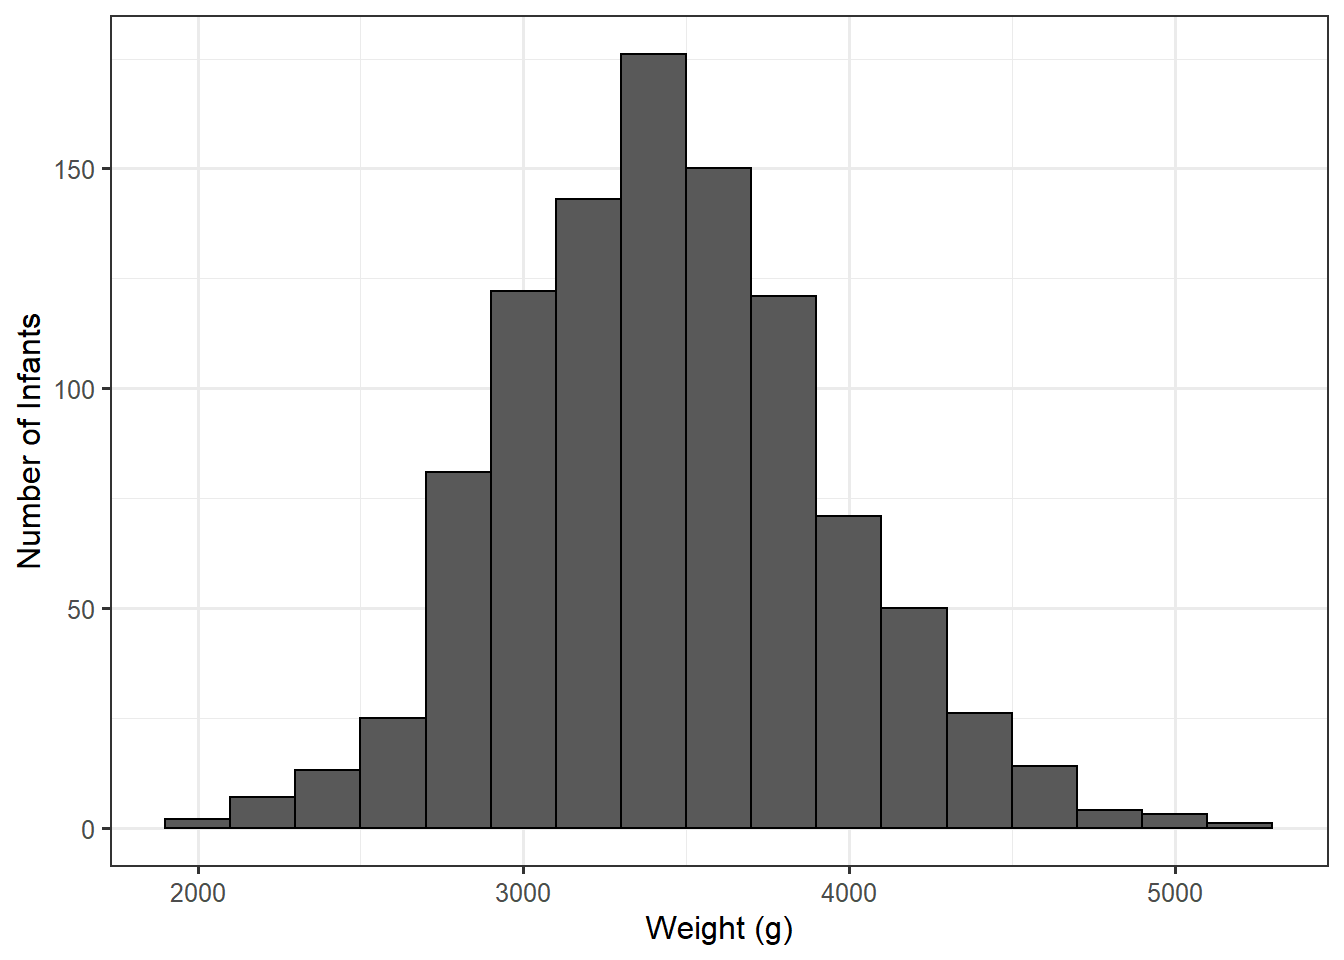
\includegraphics[width=0.8\linewidth]{./Images/singleconfint-histogram-1} 

}

\caption{Weight of infants born in North Carolina.}\label{fig:singleconfint-histogram}
\end{figure}

In order to construct an estimate of \(\mu\) which incorporates the
variability in the sample mean, we must model the sampling distribution
of our estimate. The bootstrap procedure for this case would be

\begin{enumerate}
\def\labelenumi{\arabic{enumi}.}
\tightlist
\item
  Randomly sample, with replacement, 1009 records from the original
  sample.
\item
  For this bootstrap resample, compute the mean birth weight and retain
  this value.
\item
  Repeat steps 1 and 2 many (say 5000) times.
\end{enumerate}

This process is illustrated in Table \ref{tab:singleconfint-bootstrap}.
Each row represents the birth weights for a single resample taken with
replacement from the original data. The final column is the computed
(and retained), sample mean from each resample. This is the bootstrap
statistic.

\begin{table}

\caption{\label{tab:singleconfint-bootstrap}Partial printout of first 10 bootstrap resamples and the resulting bootstrap statistic.}
\centering
\begin{tabular}[t]{r|r|r|l|r|r|r|r}
\hline
Value 1 & Value 2 & Value 3 &         & Value 1007 & Value 1008 & Value 1009 & Boostrap Mean\\
\hline
3232 & 3260 & 2948 & ... & 3232 & 2863 & 3345 & 3460.26\\
\hline
3317 & 3232 & 3090 & ... & 3629 & 3402 & 3771 & 3438.70\\
\hline
3147 & 3260 & 3714 & ... & 3119 & 3374 & 3204 & 3440.23\\
\hline
4139 & 3686 & 3912 & ... & 4281 & 3600 & 4224 & 3467.40\\
\hline
2722 & 4054 & 3175 & ... & 3629 & 3090 & 3799 & 3444.81\\
\hline
4082 & 3799 & 3459 & ... & 3742 & 4196 & 3062 & 3453.83\\
\hline
2835 & 2863 & 4394 & ... & 3090 & 3686 & 3090 & 3447.73\\
\hline
2580 & 2722 & 3969 & ... & 2835 & 4338 & 2977 & 3460.19\\
\hline
2863 & 3204 & 3430 & ... & 3232 & 3459 & 2948 & 3445.78\\
\hline
3572 & 3289 & 3345 & ... & 4224 & 3969 & 3175 & 3441.17\\
\hline
\end{tabular}
\end{table}

A plot of the resulting bootstrap sample means is shown in Figure
\ref{fig:singleconfint-samp-distn}. Notice that the x-axis is different
from that of Figure \ref{fig:singleconfint-histogram}. While a graphical
summary of the raw data is summarizing the weight of individual infants,
the sampling distribution is summarizing the statistic we compute in
various samples of the same size. We are not keeping track of individual
infant weights but average weights for collections of 1009 infants.

\begin{figure}

{\centering 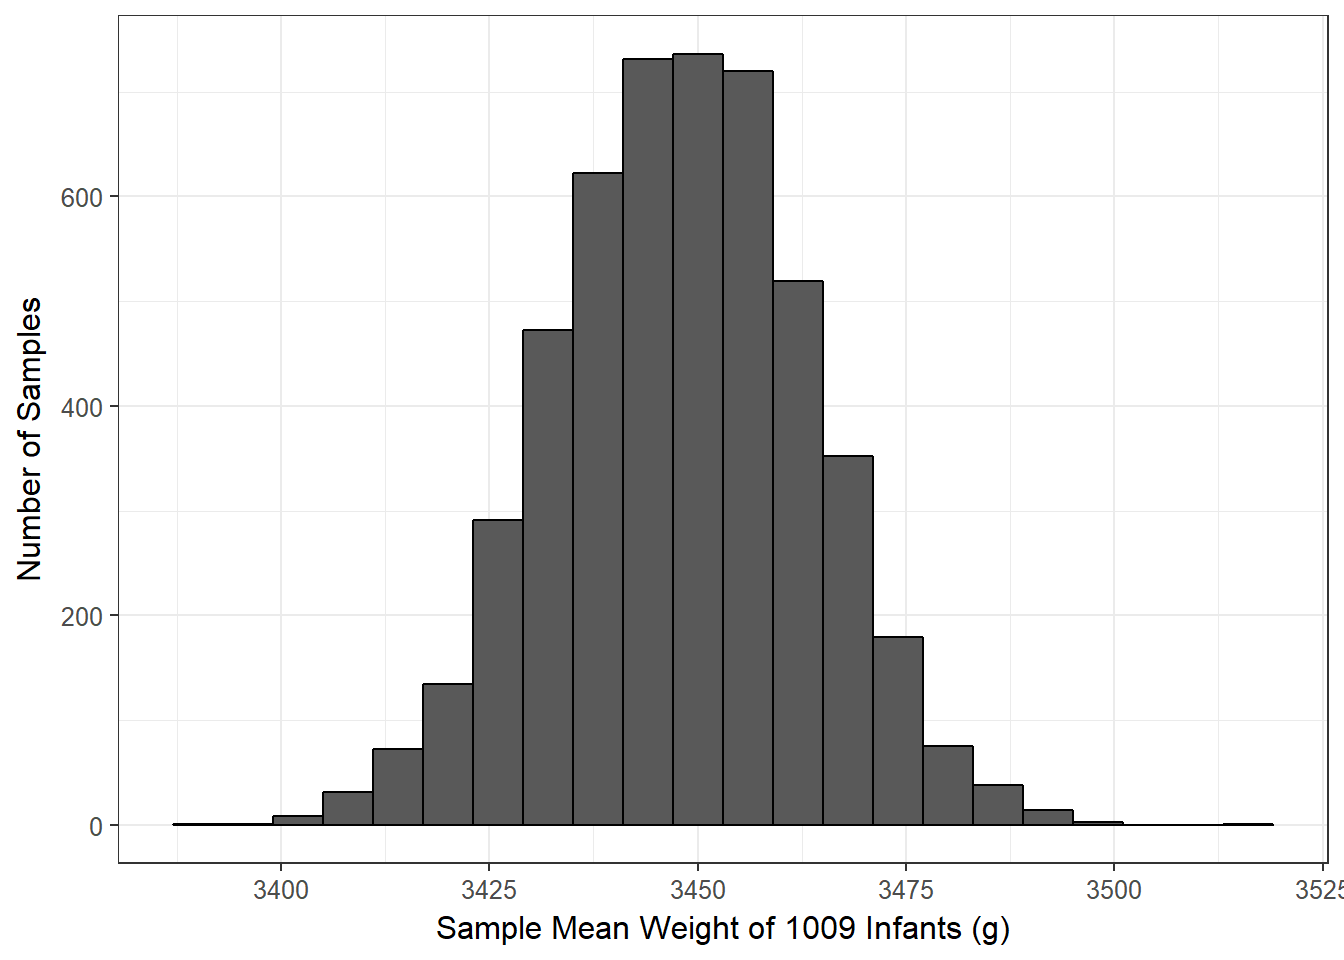
\includegraphics[width=0.8\linewidth]{./Images/singleconfint-samp-distn-1} 

}

\caption{Bootstrap model for the sampling distribution of the average birth weight for a sample of 1009 infants born in North Carolina.}\label{fig:singleconfint-samp-distn}
\end{figure}

Using this model, we can then grab the middle 95\% of values in order to
construct a confidence interval for the parameter of interest. This
results in a 95\% confidence interval of (3417.82, 3477.31). Therefore,
the data is consistent with the average birth weight of infants in North
Carolina being between 3417.82 and 3477.31; that is, these are the
reasonable values of the mean birth weight.

Notice that we are able to narrow down the reasonable values of the
parameter to a relatively small interval (a difference of about 60
grams). This is not because all babies in North Carolina have an
extremely similar birth weight. It is because we have a relatively large
sample, allowing us to have high confidence in our estimate.

Also, notice how much narrower the model for the sampling distribution
is compared to the raw data. Remember, statistics have less variability
than individual values. This also illustrates why a confidence interval
could never describe the fraction of values in the population which fall
within a certain range --- the variability is not comparable because a
sampling distribution has a different x-axis than the distribution of
the population or sample.

\chapter{Quantifying the Evidence}\label{SingleTeststat}

In the previous chapter, we estimated the mean response for a single
quantitative variable. In this chapter, we consider hypothesis testing
when the parameter of interest is the mean response for a single
quantitative variable.

Let's consider the \protect\hyperlink{CaseBabies}{Birth Weight Case
Study}. In 2004, when the data was collected, an infant was considered
``full term'' if it was born anytime between 37 and 42 weeks. However,
in 2013 the
\href{https://journals.lww.com/greenjournal/Fulltext/2013/11000/Committee_Opinion_No_579___Definition_of_Term.39.aspx}{American
College of Obstetricians and Gynecologists redefined ``full term''} to
mean an infant born anytime between 39 and 40 weeks. We will consider
the following research question:

\begin{quote}
Is there evidence that the gestation time for infants born in North
Carolina exceeds 38 weeks (so that the baby is at least full term on
average)?
\end{quote}

This question is captured by the following set of hypotheses:

\[H_0: \theta \leq 38 \qquad \text{vs.} \qquad H_1: \theta > 38\]

where \(\theta\) is the average gestation period (weeks) of an infant
born in North Carolina. This parameter is also present in the data
generating process:

\[(\text{Gestation Period})_i = \theta + \epsilon_i\]

We will assume that the gestation period for one infant is independent
of the gestation period for any other infant and that this data is
representative of all infants born in North Carolina; this implies we
can assume the errors are independent and identically distributed.

We can estimate the parameter \(\theta\) with the average gestation
period for the babies in our sample: 39.11 weeks. We seek to quantify
the evidence against the null hypothesis summarized by this data.

In Chapter \ref{NullDistns}, we developed the null distribution of the
statistic used to estimate the parameter. Following that chapter, we
would model the null distribution of the sample mean gestation for a
sample of 1009 infants. This null distribution, modeled via
bootstrapping assuming the data is consistent with the above conditions
on the error term, is shown in Figure
\ref{fig:singleteststat-null-mean}.

\begin{figure}

{\centering 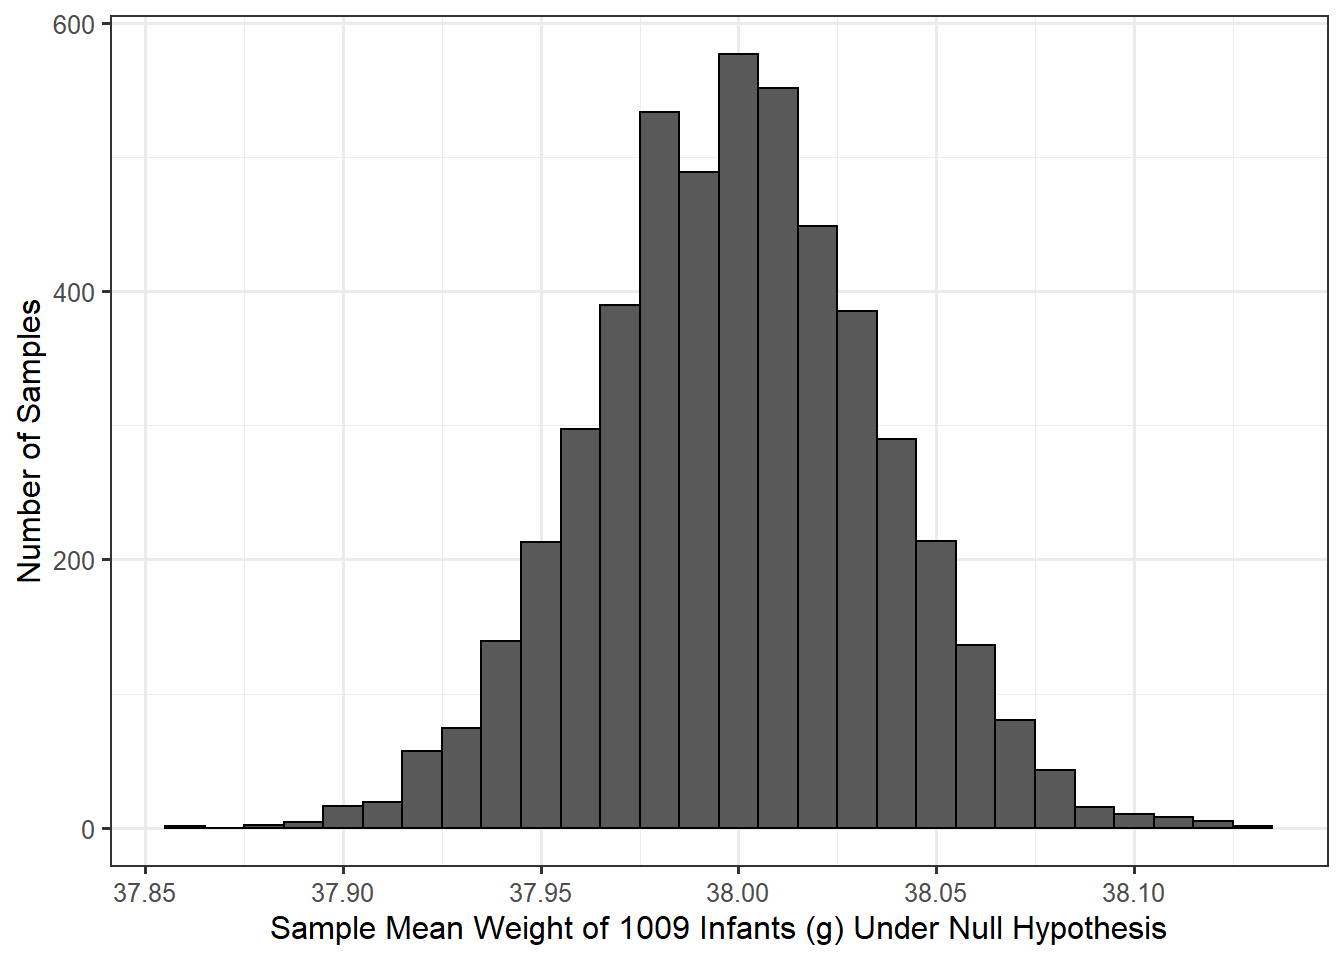
\includegraphics[width=0.8\linewidth]{./Images/singleteststat-null-mean-1} 

}

\caption{Model of the null distribution of the sample mean gestation period for a sample of 1009 infants. The model is based on 5000 bootstrap replications under the null hypothesis that the average gestation period is 38 weeks.}\label{fig:singleteststat-null-mean}
\end{figure}

This figure was constructed using the following procedure:

\begin{enumerate}
\def\labelenumi{\arabic{enumi}.}
\tightlist
\item
  Alter the sample to be representative of having come from a population
  in which the null hypothesis is true; the data was recentered to have
  a sample mean of 38.
\item
  Randomly sample, with replacement, 1009 records from the altered
  original sample.
\item
  For this bootstrap resample, compute the mean gestation period and
  retain this value.
\item
  Repeat steps 2 and 3 many (say 5000) times.
\end{enumerate}

The resulting simulated data is illustrated in Table
\ref{tab:singleteststat-bootstrap-mean}. Each row represents the
gestation periods for a single resample taken with replacement from the
altered original data. The final column is the computed (and retained),
sample mean from each resample. This is the bootstrap statistic
\emph{under the null hypothesis}.

\begin{table}

\caption{\label{tab:singleteststat-bootstrap-mean}Partial printout of first 10 bootstrap resamples under the null hypothesis and the resulting bootstrap statistic.}
\centering
\begin{tabular}[t]{r|r|r|l|r|r|r|r}
\hline
Value 1 & Value 2 & Value 3 &         & Value 1007 & Value 1008 & Value 1009 & Boostrap Mean\\
\hline
37.89 & 36.89 & 36.89 & ... & 38.89 & 39.89 & 37.89 & 37.92\\
\hline
39.89 & 38.89 & 39.89 & ... & 37.89 & 37.89 & 36.89 & 38.00\\
\hline
36.89 & 37.89 & 36.89 & ... & 37.89 & 37.89 & 37.89 & 38.02\\
\hline
39.89 & 37.89 & 38.89 & ... & 36.89 & 36.89 & 37.89 & 37.99\\
\hline
38.89 & 38.89 & 38.89 & ... & 39.89 & 36.89 & 36.89 & 38.04\\
\hline
38.89 & 39.89 & 37.89 & ... & 36.89 & 36.89 & 36.89 & 37.99\\
\hline
37.89 & 38.89 & 37.89 & ... & 36.89 & 36.89 & 35.89 & 38.01\\
\hline
37.89 & 37.89 & 38.89 & ... & 37.89 & 39.89 & 37.89 & 38.02\\
\hline
37.89 & 37.89 & 36.89 & ... & 36.89 & 37.89 & 38.89 & 37.99\\
\hline
37.89 & 37.89 & 39.89 & ... & 37.89 & 37.89 & 37.89 & 37.97\\
\hline
\end{tabular}
\end{table}

Notice that the null distribution is centered on 38; this is not an
accident. Recall that sampling distributions are centered on the true
value of the parameter; since a null distribution is just the sampling
distribution when the parameter is equal to the null value (in this case
38), it should be centered on the null value. That is, the null
distribution is designed to be centered on the null value in the
hypotheses. In order to determine if our sample is consistent with our
expectations, we overlay our observed sample mean
(\(\widehat{\theta} = 39.11\)) on the null distribution. Since this
value is in the far right tail of the null distribution (off the edge of
the graph in this case), our sample is \emph{inconsistent} with the null
distribution. That is, we have evidence that the population from which
our sample was drawn has an average gestation period larger than 38
weeks.

\section{Standardized Statistics}\label{standardized-statistics}

In the above discussion, we compared the observed sample mean to our
distribution of expectations if the null hypothesis were true. We were
essentially comparing \(\widehat{\theta}\) to 38 while accounting for
the sampling variability of our estimate \(\widehat{\theta}\), the
sample mean. This is a completely valid approach to inference. In this
section, we consider an equivalent (conceptually), though alternative,
approach which will provide a more general framework for inference.

At its heart, hypothesis testing is about comparing two models for the
data generating process. So far, we have stated one of those models:

\[\text{Model 1}: \quad (\text{Gestation Period})_i = \theta + \epsilon_i\]

This is the data generating process under the alternative hypothesis in
which no restrictions are placed on the value of \(\theta\). However,
\emph{if} the null hypothesis is true, then the model for the data
generating process simplifies to

\[\text{Model 0}: \quad (\text{Gestation Period})_i = 38 + \epsilon_i\]

This may not seem like a simpler model, but it is because there are less
(in this case none) unknown parameters. A null hypothesis essentially
places further restrictions on the data generating process. A hypothesis
test is then about comparing these two models.

\BeginKnitrBlock{rmdkeyidea}
Hypothesis testing is about comparing two models for the data generating
process.
\EndKnitrBlock{rmdkeyidea}

The hypotheses we have been considering in this chapter could be
rewritten as:

\[
\begin{aligned}
  H_0: \text{Model 0 is sufficient for explaining the data observed.} \\
  H_1: \text{Model 0 is not sufficient for explaining the data observed.}
\end{aligned}
\]

That is, when conducting a hypothesis test, we are really determining
whether the data provides evidence that the model for the data
generating process under the null hypothesis is sufficient for
explaining the observed data. This is why we refer to hypothesis testing
as assessing model consistency. We are determining if there is evidence
that the data is inconsistent with a proposed model for the data
generating process.

Intuitively, the two proposed models would be equivalent (Model 0 would
be sufficient for explaining the data) if they both performed similarly
in predicting a response. Model 1 would be preferred (Model 0 would not
be sufficient for explaining the data) if it performs better in
predicting the response. We can assess ``prediction'' by the amount of
variability in the data. For Model 0, the amount of variability can be
quantified by

\[SS_0 = \sum_{i=1}^{n} \left[(\text{Gestation Period})_i - 38\right]^2\]

For Model 1, the amount of variability can be quantified by

\[SS_1 = \sum_{i=1}^{n} \left[(\text{Gestation Period})_i - \widehat{\theta}\right]^2\]

where \(\widehat{\theta} = 39.11\), the observed sample mean. Notice
that these sums of squared (SS) terms are similar to the definition of
sample variance discussed in Chapter \ref{Summaries}, without the
scaling factor. The rationale for using these to assess predictive
ability of the model will be further discussed in a later chapter. Here,
we simply note that they are measuring a distance the observed data is
from a mean; the difference is whether that mean is unrestricted (and
therefore estimated from the data, Model 1) or restricted under the null
hypothesis (Model 0). If \(SS_0\) and \(SS_1\) were similar, then it
would suggest that \(\widehat{\theta}\) differs from the null value only
due to sampling variability, which would be in line with the null
hypothesis. If, on the other hand, \(SS_0\) and \(SS_1\) differ
substantially from one another, it suggests \(\widehat{\theta}\) differs
from the null value more than we would expect due to variability alone.
Therefore, the difference in these two sums of squares gives us a
measure of the signal in the data against the null hypothesis. The
larger this difference, the stronger the signal.

Unfortunately, the difference between these two values alone is not
sufficient. That is, a signal is not enough without knowing the
background noise. Think about having a radio on in the background of a
party, and suppose the radio is set to a specific volume. If there are
not many people talking at the party, it is easy to hear the radio; the
signal is strong relative to the background noise. However, if there are
a lot of people talking at the party, the radio is difficult to hear
even though its volume hasn't changed; the signal is weak
\emph{relative} to the background noise. A signal is more difficult to
locate if the background noise is elevated. The same principle holds in
data analysis.

Consider Figure \ref{fig:singleteststat-signal-to-noise}. Suppose we
want to use each of these datasets (both containing a sample of size
\(n = 20\)) to test the hypotheses:

\[H_0: \mu = 0 \qquad \text{vs.} \qquad H_1: \mu \neq 0\]

where \(\mu\) is the population mean. Both datasets have \emph{exactly}
the same observed sample mean response (the black diamond in the
figure). Therefore, it can be shown that the difference between \(SS_0\)
and \(SS_1\) is exactly the same for both datasets. However, just
visually, it should be clear that Dataset A provides stronger evidence
against the null hypothesis than Dataset B; that is, Dataset A is more
inconsistent with a mean of 0. What is the difference? The variability;
the background noise.

\begin{figure}

{\centering 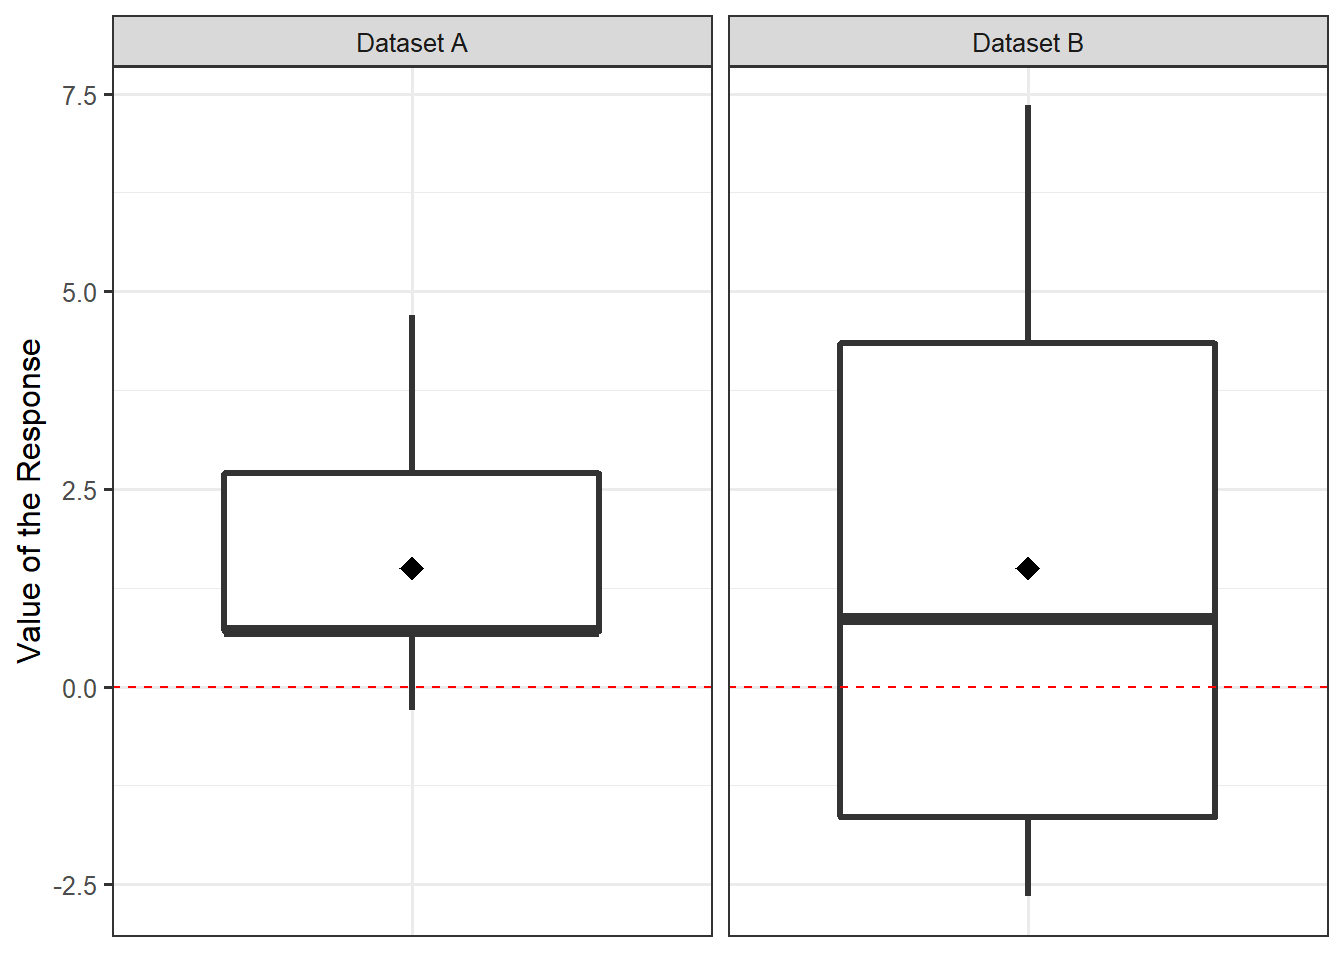
\includegraphics[width=0.8\linewidth]{./Images/singleteststat-signal-to-noise-1} 

}

\caption{Illustration of the need to compare a signal to the noise in the data to assess its true strength.}\label{fig:singleteststat-signal-to-noise}
\end{figure}

Therefore, when quantifying the strength of a signal in a statistical
analysis, it is common to measure the signal relative to the background
noise. Returning to our example for the
\protect\hyperlink{CaseBabies}{Birth Weight Case Study}, we have that
\(SS_0 - SS_1\) is our signal. The noise is the variability in the
sample

\[s^2 = \frac{1}{n-1}\sum_{i=1}^{n} \left[(\text{Gestation Period})_i - \widehat{\theta}\right]^2\]

as measured by the sample variance. Our signal-to-noise ratio is then

\[T^* = \frac{SS_0 - SS_1}{s^2} = 963.2\]

for our example. Such signal to noise ratios are known as
\textbf{standardized statistics}.

\BeginKnitrBlock{definition}[Standardized Statistic]
\protect\hypertarget{def:defn-standardized-test-statistic}{}{\label{def:defn-standardized-test-statistic}
\iffalse (Standardized Statistic) \fi{} }A ratio of the signal of the
sample and the noise in the sample. The larger the test statistic, the
stronger the evidence of a signal; said another way, the larger the test
statistic, the stronger the evidence against the null hypothesis.
\EndKnitrBlock{definition}

\BeginKnitrBlock{rmdtip}
A standardized statistic is often refered to as a ``standardized test
statistic'' because they are heavily used in hypothesis testing.
\EndKnitrBlock{rmdtip}

Just as we constructed the null distribution for the observed sample
mean in order to construct a distribution of our expectations under the
null hypothesis, we can construct a null distribution of the
standardized statistic to determine our expectations of this ratio under
the null hypothesis. Figure \ref{fig:singleteststat-null} provides a
model for this distribution. This is constructed in the same way as we
did the null distribution for the sample mean except that instead of
retaining the sample mean from each resample, we compute and retain the
standardized statistic from each resample.

\begin{figure}

{\centering 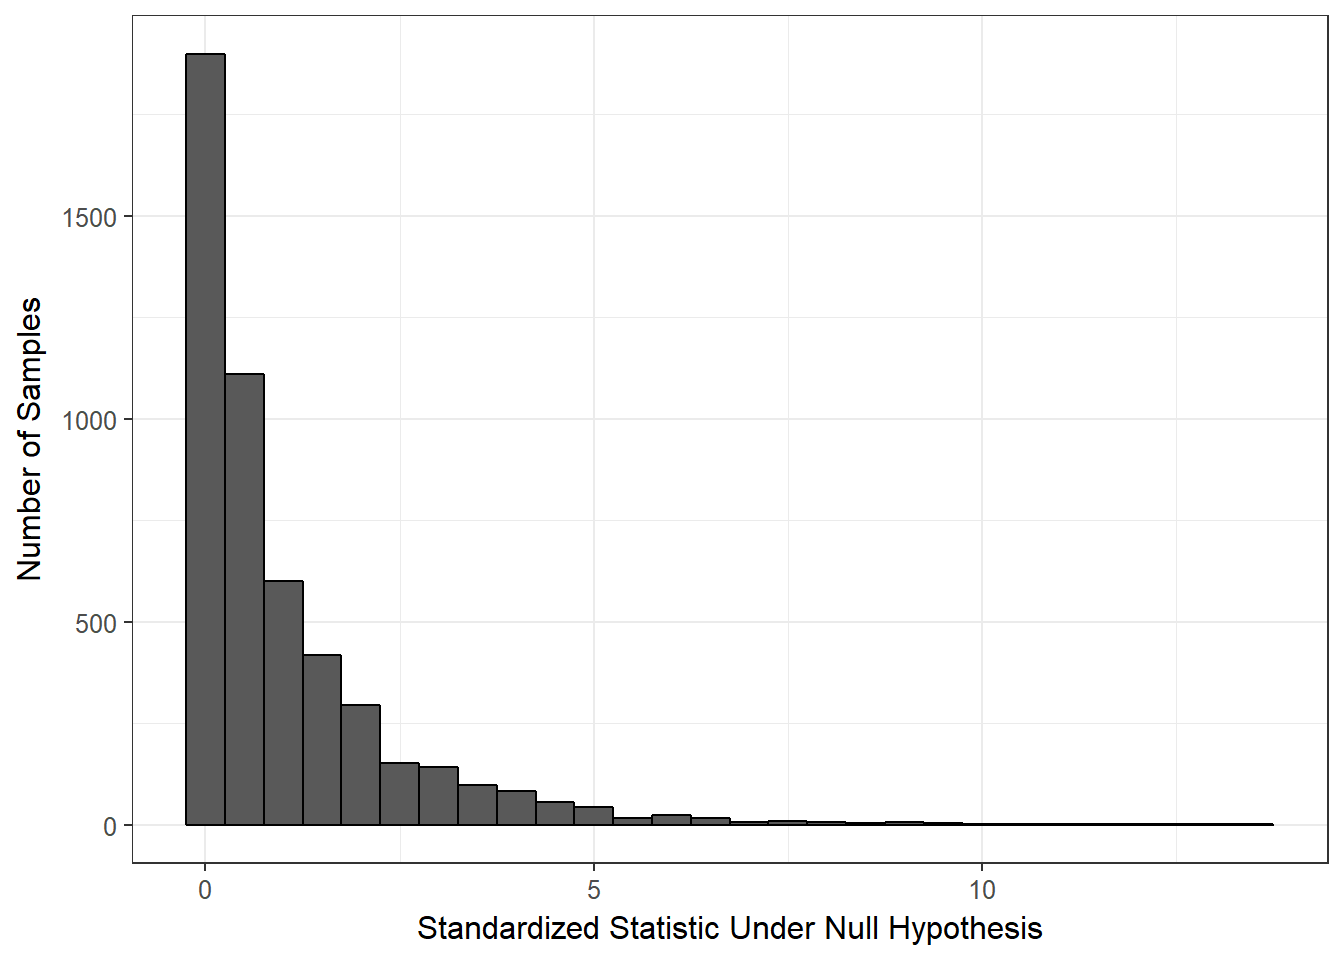
\includegraphics[width=0.8\linewidth]{./Images/singleteststat-null-1} 

}

\caption{Model of the null distribution of the standardized statistic for a sample of 1009 infants. The model is based on 5000 bootstrap replications under the null hypothesis that the average gestation period is 38 weeks.}\label{fig:singleteststat-null}
\end{figure}

Notice that we reach the same conclusions. Our data is inconsistent with
null hypothesis because our observed test statistic of 963.2 is in the
far right tail of the null distribution. That is, if the null
distribution were true, it would be very unlikely to obtain a sample
which was this extreme due to sampling variability alone.

So, if our conclusions do not change, why the two different approaches?
It turns out there is some theory that says bootstrapping standardized
statistics tends to behave computationally a bit better, and these
standardized statistics are a bit easier to model analytically using
probability theory. We prefer talking about them because it again
provides a nice overarching framework.

\BeginKnitrBlock{rmdkeyidea}
Quantifying evidence compares the signal in the data to the noise.
\EndKnitrBlock{rmdkeyidea}

Before moving on, we should note that there is not a unique standardized
statistic. Other standardized statistics are often quoted, such as

\[\frac{\sqrt{n}\left(\widehat{\theta} - 38\right)}{s}\]

It can be shown that many such standardized statistics are related to
the one we have described above (this one is the square root of that
described above, for example). When the same conditions are applied,
various standardized statistics yield the same results. Again, we opt
for the one described earlier because it will provide continuity in the
text.

\section{Computing the P-value}\label{computing-the-p-value}

Now that we have a model for the null distribution of the standardized
statistic, we can compute a p-value. The p-value is the probability of
observing a sample more extreme due only to sampling variability. Our
standardized statistic has the form

\[T^* = \frac{SS_0 - SS_1}{s^2}\]

If the sample were more extreme --- that is, if it produced a larger
signal --- then we would expect the difference between \(SS_0\) and
\(SS_1\) to be even larger. Therefore, larger values of the standardized
statistic present stronger evidence of the data. So, when looking at the
null distribution of the standardized statistic, computing the p-value
corresponds to computing the area to the right of the observed
standardized statistic.

Looking back at Figure \ref{fig:singleteststat-null}, our observed
standardized statistic is not even on the graphic, meaning the p-value
would be essentially 0. The data therefore provides strong evidence that
the average gestation period of infants born in North Carolina exceeds
38 weeks.

\part{Unit III: Modeling the Average Response as a Function
of a Continuous
Predictor}\label{part-unit-iii-modeling-the-average-response-as-a-function-of-a-continuous-predictor}

\hypertarget{CaseGreece}{\chapter{Case Study: Seismic Activity in
Greece}\label{CaseGreece}}

At the intersection of the African plate, the Eurasia plate, and the
smaller Aegean plate, Greece is one of the most earthquake-prone regions
in the world. Between July 2016 and July 2017, Greece experienced 179
earthquakes; by contrast, the state of Texas experienced 28 over the
same span of time. In a region with such seismic activity, careful
consideration must be given to municipal construction. Further,
understanding how the motion experienced in a location is related to the
soil properties in the area or the magnitude and distance of an
earthquake is important.

An article in the \emph{Journal of Earthquake Engineering} (Koutrakis et
al. \protect\hyperlink{ref-Koutrakis2002}{2002}) examined seismic events
in Greece occurring between 1978 and 1997. Of interest for construction
is characterizing the ``strong ground motion,'' when the earth shakes
with enough force to cause damage to infrastructure, with respect to the
properties of a location. The study recorded several measurements from
121 stations (representing 93 distinct seismic events)\footnote{The
  original article presented repeated measurements at each location. We
  present here only the first measurement from each location to simplify
  any analyses. Repeated measurements are discussed briefly later in the
  text; for a more thorough treatment of the subject, we recommend a
  course in Designed Experiments or Biostatistics. The dataset presented
  here corresponds to that presented in Navidi's ``Statistics for
  Engineers and Scientists'' (Chapter 8, Supplementary Exercise 22).}.
The primary variable of interest is the \emph{bracketed duration}, ``the
time interval {[}in seconds{]} between the first and last excursion of
the peak ground acceleration beyond a certain predefined level.'' For
our purposes, we only consider the data corresponding to a threshold of
2\% of the acceleration due to gravity. In addition, the following
measurements were available for each observation:

\begin{itemize}
\tightlist
\item
  Moment Magnitude: a measure of the size of the earthquake; larger
  values indicate more severe earthquakes.
\item
  Epicentral Distance: distance (kilometers) from the epicenter of the
  earthquake to the location at which the measurement was taken.
\item
  Soil Condition: indicator of the type of soil present at the
  measurement site. Soil was categorized as one of three types -
  alluvium (soft, fine particles of clay, silt, sand, and gravel),
  intermediate soil conditions, or tertiary or older rock (those older
  than 2.58 million years).
\end{itemize}

The first 5 observations in the dataset are shown in Table
\ref{tab:casegreece-table}. We are interested in characterizing the
relationship between bracketed duration and the magnitude of the
earthquake.

\begin{table}

\caption{\label{tab:casegreece-table}Data for first 5 observations from study characterizing seismic activity in Greece.}
\centering
\begin{tabular}[t]{r|r|r|l}
\hline
Magnitude & Distance from Epicenter (km) & Bracketed Duration (s) & Soil Conditions\\
\hline
6.4 & 30 & 8.82 & Soft\\
\hline
5.3 & 6 & 4.31 & Intermediate\\
\hline
5.6 & 15 & 5.74 & Intermediate\\
\hline
5.2 & 7 & 4.08 & Intermediate\\
\hline
6.6 & 31 & 28.27 & Soft\\
\hline
\end{tabular}
\end{table}

\chapter{Myriad of Potential Questions}\label{Regquestions}

For the \protect\hyperlink{CaseGreece}{Seismic Activity Case Study}, we
are primarily interested in characterizing the relationship between
bracketed duration and the magnitude of the earthquake. First, note that
this question is about the relationship between a quantitative response
(bracketed duration; see Definition \ref{def:defn-response}) and a
quantitative predictor (magnitude). Also note that the question is quite
broad. We might actually have one of the following more specific ideas
in mind:

\begin{itemize}
\tightlist
\item
  In general, does the bracketed duration increase as the magnitude
  increases?
\item
  If two earthquakes with different magnitudes occur in the same
  location, would we expect the same bracketed duration regardless of
  their magnitudes?
\item
  Is the relationship between the bracketed distance and the magnitude
  different depending on the soil condition of where the measurement is
  taken?
\end{itemize}

These illustrate an array of potential questions we could address with
the data. Each represents a different emphasis that we might have in a
research question:

\begin{itemize}
\tightlist
\item
  Marginal Relationship: overall, do two variables tend to move together
  (are they correlated)?
\item
  Isolation of Effect: does a relationship exist after accounting for
  the effect of additional variables? Or, what is the effect ``above and
  beyond'' the effect of additional variables?
\item
  Interplay: how does the relationship between two variables change as a
  result of a third?
\end{itemize}

There is no right question to ask; each question examines a different
facet of the relationship between two quantitative variables. In this
unit, we will focus on questions of the first type. However, the
framework we introduce is broad enough to be extended to address each of
these types of questions. This may sound daunting, but keep in mind that
the fundamental ideas we discussed in Unit I and applied in Unit II will
continue to form the foundation of the analyses discussed in this unit;
namely,

\begin{itemize}
\tightlist
\item
  We are using a sample to say something about the underlying
  population.
\item
  In order to make inference, we will need a model for the sampling (or
  null) distribution of our statistic.
\item
  In order to form a standardized statistic of interest which measures
  the strength of the signal in the dataset, we think about variability.
\end{itemize}

The ideas remain the same; the context has changed. Stating these
questions mathematically will require us to extend the model for the
data-generating process we developed in Unit 2.

There is one more thing we want to point out before moving on: any
relationships we observe are overall trends, not guaranteed to hold for
any single individual. Recall that in Unit II we emphasized that our
conclusions were about the mean response (the parameter of interest).
Specifically, even if we know the average response within the
population, due to variability, we do not expect every individual to
have that specific value for the response. This will continue in this
unit. If we observe, for example, that an increase in the magnitude is
associated with an increase in the bracketed duration, we are describing
an overall trend. It is highly likely there is some location for which
this trend does not hold, simply due to variability.

\chapter{Nature of Collecting Multivariable Data}\label{Regdata}

For the \protect\hyperlink{CaseGreece}{Seismic Activity Case Study}, we
are primarily interested in characterizing the relationship between
bracketed duration and the magnitude of the earthquake. As we discussed
in the previous chapter, this general goal might be refined into one of
many specific questions:

\begin{itemize}
\tightlist
\item
  In general, does the bracketed duration increase as the magnitude
  increases?
\item
  If two earthquakes with different magnitudes occur in the same
  location, would we expect the same bracketed duration regardless of
  their magnitudes?
\item
  Is the relationship between the bracketed distance and the magnitude
  different depending on the soil condition of where the measurement is
  taken?
\end{itemize}

Notice that these last two questions actually require knowledge of more
than just the braketed duration and the magnitude of each seismic event.
In order to address the second question, we would also need the distance
from the center of the earthquake; in order to address the third
question, we also need the soil conditions of where the measurement is
taken. Often, research questions require knowledge of more than just a
single variable; such questions are \textbf{multivariable}.

\BeginKnitrBlock{definition}[Multivariable]
\protect\hypertarget{def:defn-multivariable}{}{\label{def:defn-multivariable}
\iffalse (Multivariable) \fi{} }Refers to questions of interest which
involve more than a single variable. Often, these questions involve many
variables.
\EndKnitrBlock{definition}

Consider going to the doctor because you are feeling ill. The doctor
does not have you simply enter your most prominent symptom (fever, for
example) into a computer and then prescribe a medication based solely on
that single symptom. Instead, a good physician will review all symptoms
you are experiencing, as well as your medical history, other
medications, allergies, etc. The physician operates in a multivariable
world in which there are many contributing factors to a response.
Therefore, when you arrive for this hypothetical visit, they record
several variables which may be of interest.

Studies which collect several variables can be observational studies or
controlled experiments. If an observational study, we want to ensure the
sample of subjects is representative of the target population. Then, for
each individual, we simply record several variables. If a controlled
experiment, we randomly assign subjects to a particular treatment group;
afterwards, we would measure the response in addition to other
variables. Notice that with the latter, subjects are randomly assigned
to only one of the variables; the remaining variables are simply
observed.

\BeginKnitrBlock{rmdtip}
When a study is primarily interested in characterizing the relationship
between two or more quantitative variables, the data is typically from
an observational study.
\EndKnitrBlock{rmdtip}

What we want to emphasize here is that how we collect the data has not
really changed from what we have discussed in previous units. The
primary difference is that we are very aware that we are collecting
several measurements on each subject. The critical element is that our
sample be representative of the target population if we want to apply
any findings to that population.

\chapter{Summarizing Multivariable Data}\label{Regsummaries}

For the \protect\hyperlink{CaseGreece}{Seismic Activity Case Study}, we
are primarily interested in characterizing the relationship between
bracketed duration and the magnitude of the earthquake. As we discussed
in the previous chapters, this broad question could be refined into a
question falling into one of three categories:

\begin{itemize}
\tightlist
\item
  Marginal Relationship: overall, do two variables tend to move together
  (are they correlated)?
\item
  Isolation of Effect: does a relationship exist after accounting for
  the effect of additional variables? Or, what is the effect ``above and
  beyond'' the effect of additional variables?
\item
  Interplay: how does the relationship between two variables change as a
  result of a third?
\end{itemize}

As always, the key is developing summaries which help to address the
question of interest.

\section{Characterizing the Marginal Relationship of Two Quantitative
Variables}\label{characterizing-the-marginal-relationship-of-two-quantitative-variables}

Suppose we are interested in the following question:

\begin{quote}
In general, does the bracketed duration increase as the magnitude
increases?
\end{quote}

This question is about the overall relationship between these two
quantitative variables. Graphically, we can examine the relationship
between these two variables using a \emph{scatter plot}. The response is
placed on the y-axis and the predictor along the x-axis. Figure
\ref{fig:regsummaries-magnitude} illustrates the relationship between
the bracketed duration and the magnitude.

\begin{figure}

{\centering 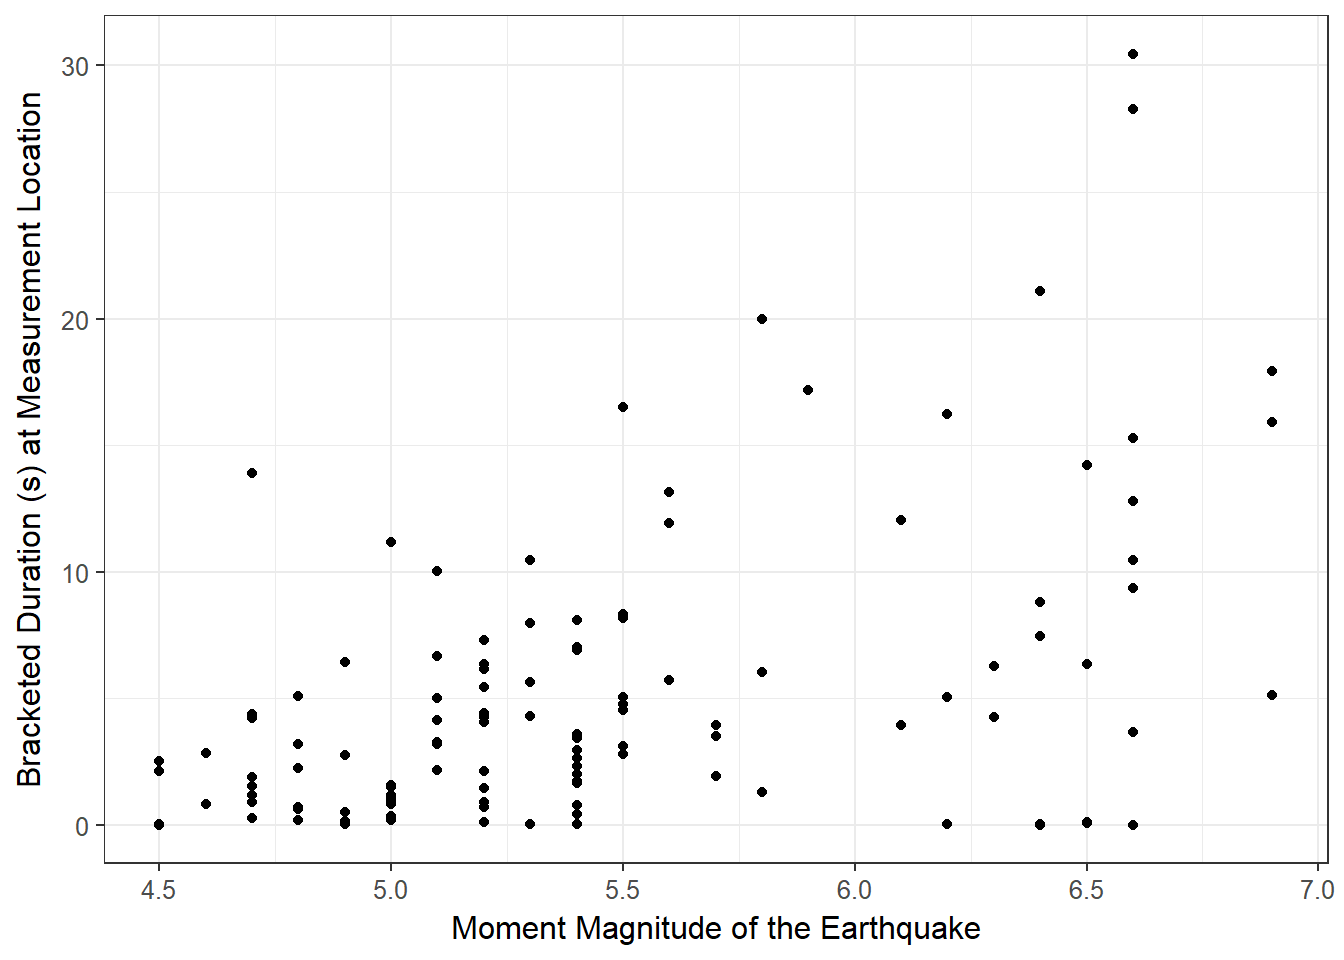
\includegraphics[width=0.8\linewidth]{./Images/regsummaries-magnitude-1} 

}

\caption{Relationship between the bracketed duration and the magnitude of an earthquake for locations Greece.}\label{fig:regsummaries-magnitude}
\end{figure}

The graphic highlights several components of the relationship. First, we
note that as the magnitude of the event increases, the bracketed
duration also tends to increase. This is intuitive --- as the size of
the earthquake increases, the length of time the ground shakes with
extreme force increases. This is a \emph{trend}; it is not a universal
truth. There are cases for which the magnitude was high, but the
bracketed duration was lower. Our goal is to characterize the overall
trend. We also notice that as the magnitude increases, the variability
in the bracketed duration also tends to increase. That is, for
earthquakes of small magnitudes, it seems fairly easy to anticipate the
bracketed duration; however, the bracketed duration is much more
difficult to anticipate for larger magnitudes.

A nice visual tool when exploring the relationship between two
quantitative variables is a \emph{smoothing spline}. The details of its
construction are beyond the scope of this text, but we can think of it
as representing where the response tends to be located for a particular
value of the predictor and then smoothing that relationship out (hence
the name). We do want to point out that this is an exploratory device;
we should be cautious about over-emphasizing relationships we observe
from the spline. Figure \ref{fig:regsummaries-spline} illustrates a
spline for the \protect\hyperlink{CaseGreece}{Seismic Events Case
Study}. The addition of the spline confirms what we had previously
stated about the relationship appearing fairly linear (as the magnitude
of the earthquake increases so does the bracketed duration at a
location). In addition to the spline, there is a confidence band
(generalization of a confidence interval) around the line in order to
convey the variability in the estimated smoothing spline.

\begin{figure}

{\centering 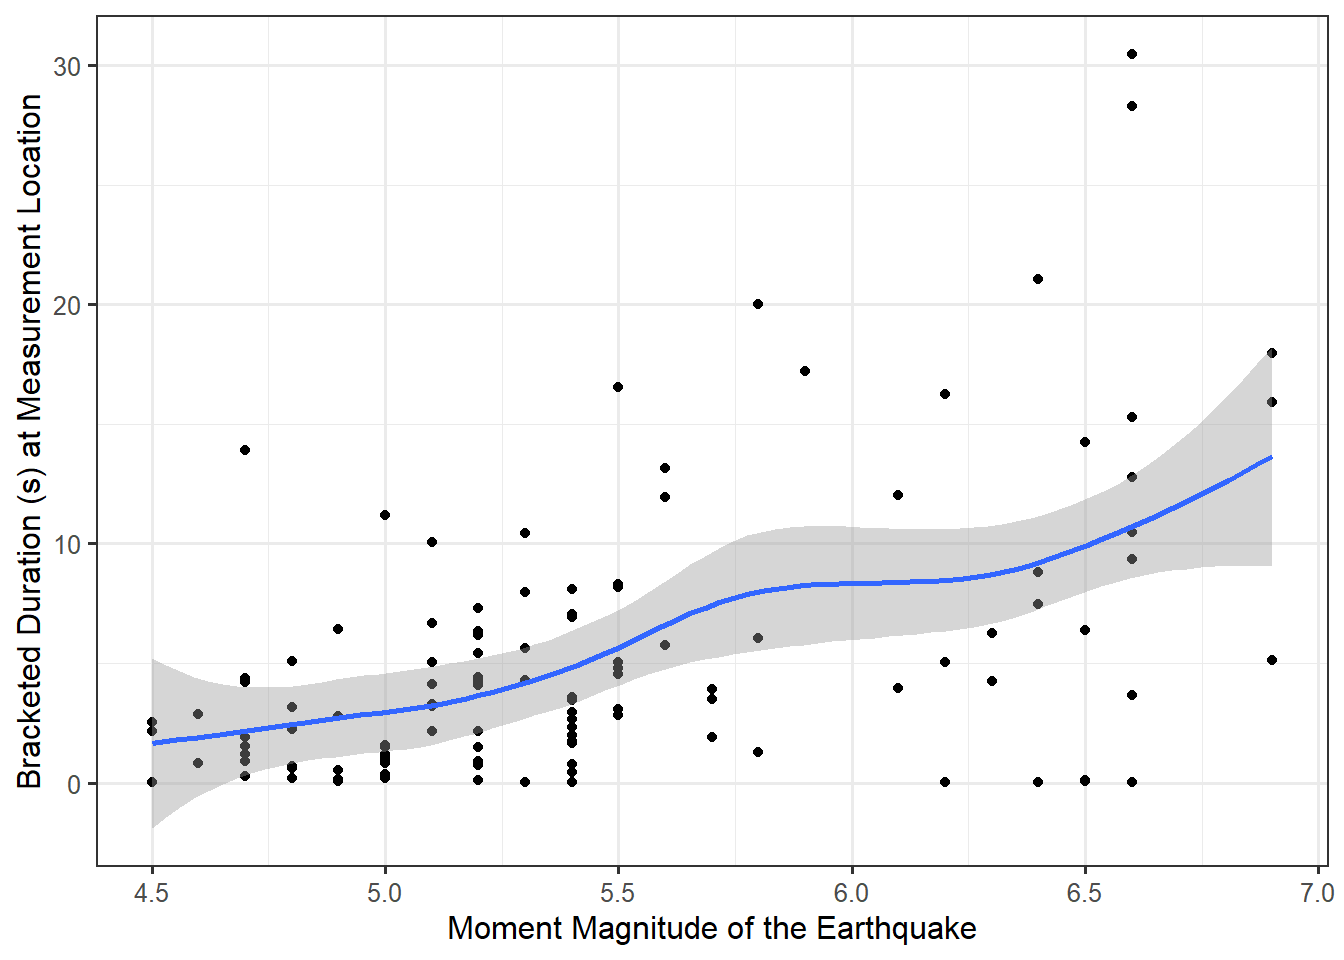
\includegraphics[width=0.8\linewidth]{./Images/regsummaries-spline-1} 

}

\caption{Illustrating the use of a smoothing spline to explore the relationship between the bracketed duration and the magnitude of an earthquake for locations Greece.}\label{fig:regsummaries-spline}
\end{figure}

As we have seen, supplementing graphical summaries with numerical
summaries can help convey our message. As an example, there is a
positive linear relationship between the response and predictor in each
of the cases illustrated in Figure \ref{fig:regsummaries-correlation}.
However, that relationship is much stronger or more apparent for Dataset
A compared to Dataset B, for example. It would be nice to have a numeric
summary which captured this; such a metric is known as the
\textbf{correlation coefficient}.

\begin{figure}

{\centering 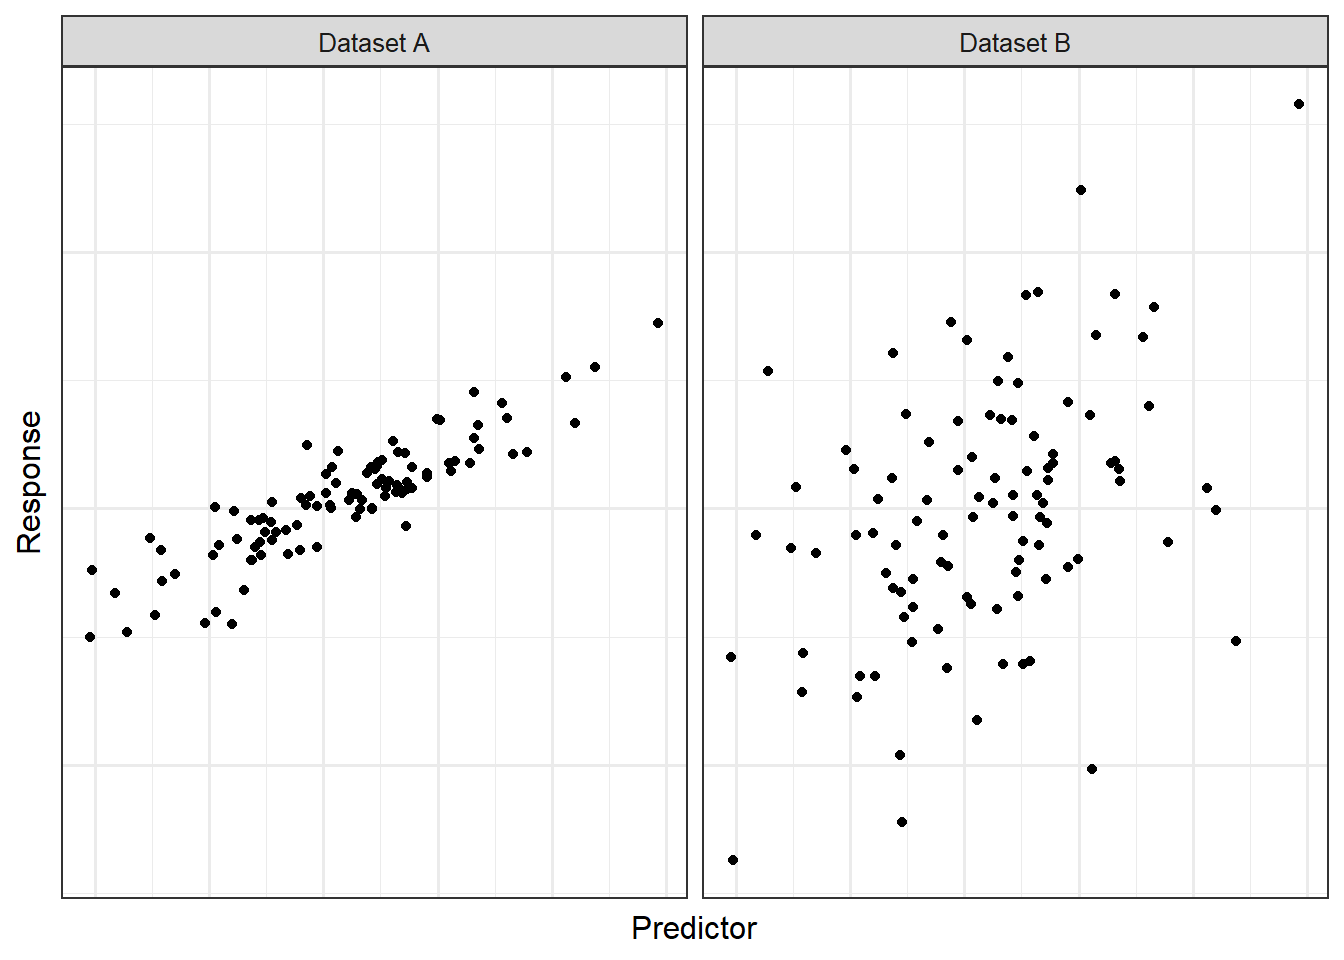
\includegraphics[width=0.8\linewidth]{./Images/regsummaries-correlation-1} 

}

\caption{Pairs of hypothetical variables which exhibit different correlations; that is, the relationship between each pair exhibit different strengths.}\label{fig:regsummaries-correlation}
\end{figure}

\BeginKnitrBlock{definition}[Correlation Coefficient]
\protect\hypertarget{def:defn-correlation-coefficient}{}{\label{def:defn-correlation-coefficient}
\iffalse (Correlation Coefficient) \fi{} }A numerical measure of the
\emph{strength} and \emph{direction} of the \emph{linear} relationship
between two quantitative variables.

The classical Pearson Correlation Coefficient \(r\) is given by the
following formula:
\[r = \frac{\sum_{i=1}^{n} \left(x_i - \bar{x}\right)\left(y_i - \bar{y}\right)}{\sqrt{\sum_{i=1}^n \left(x_i - \bar{x}\right)^2 \sum_{i=1}^n \left(y_i - \bar{y}\right)^2}}\]

where \(\bar{x}\) and \(\bar{y}\) represent the sample means of the
predictor and response, respectively.
\EndKnitrBlock{definition}

The correlation between the bracketed duration and the magnitude of an
earthquake is 0.497, indicating the two variables are positively
linearly related, though perhaps the relationship is not strong.

\BeginKnitrBlock{rmdtip}
Correlation coefficients measure both the strength and direction of
linear relationships. Here are a few of their key properties:

\begin{itemize}
\tightlist
\item
  Takes a value between -1 and 1.
\item
  Negative values mean that the variables tend to move in opposite
  directions.
\item
  Positive values mean that the variables tend to move in the same
  direction.
\item
  Unitless and therefore unaffected by unit changes in the variables.
\end{itemize}

The biggest thing to remember is that a correlation coefficient measures
the strength of a \emph{linear} relationship. A correlation of 0 does
not mean that two variables are unrelated. It simply means they are not
linearly related.
\EndKnitrBlock{rmdtip}

\section{Visualizing the Impact of a Third Variable on the Marginal
Relationship}\label{visualizing-the-impact-of-a-third-variable-on-the-marginal-relationship}

In the previous section, we stated that the bracketed duration tended to
increase as the magnitude increased. It is reasonable to ask the
following question:

\begin{quote}
Is the relationship between the bracketed distance and the magnitude
different depending on the soil condition of where the measurement is
taken?
\end{quote}

That is, we want to determine the impact that a third variable (soil
condition) has on the relationship we have observed. While the bulk of
this unit will focus on inferential methods for the marginal
relationship, graphically assessing questions isolating a single
predictor or about the interplay of two predictors is fairly intuitive.
In order to add more depth to our graphical representations, we make use
of various attributes of the graphic: color of the points used in
plotting, shape of the points used in plotting, size of the points used
in plotting, facets (multiple graphics each with a different subset of
the data). Figure \ref{fig:regsummaries-color} uses color to distinguish
between the three possible types of soil conditions of the measurement
locations. Notice the graphic allows us to both visualize the
relationship for each soil condition but also facilitates our comparing
these relationships.

\begin{figure}

{\centering 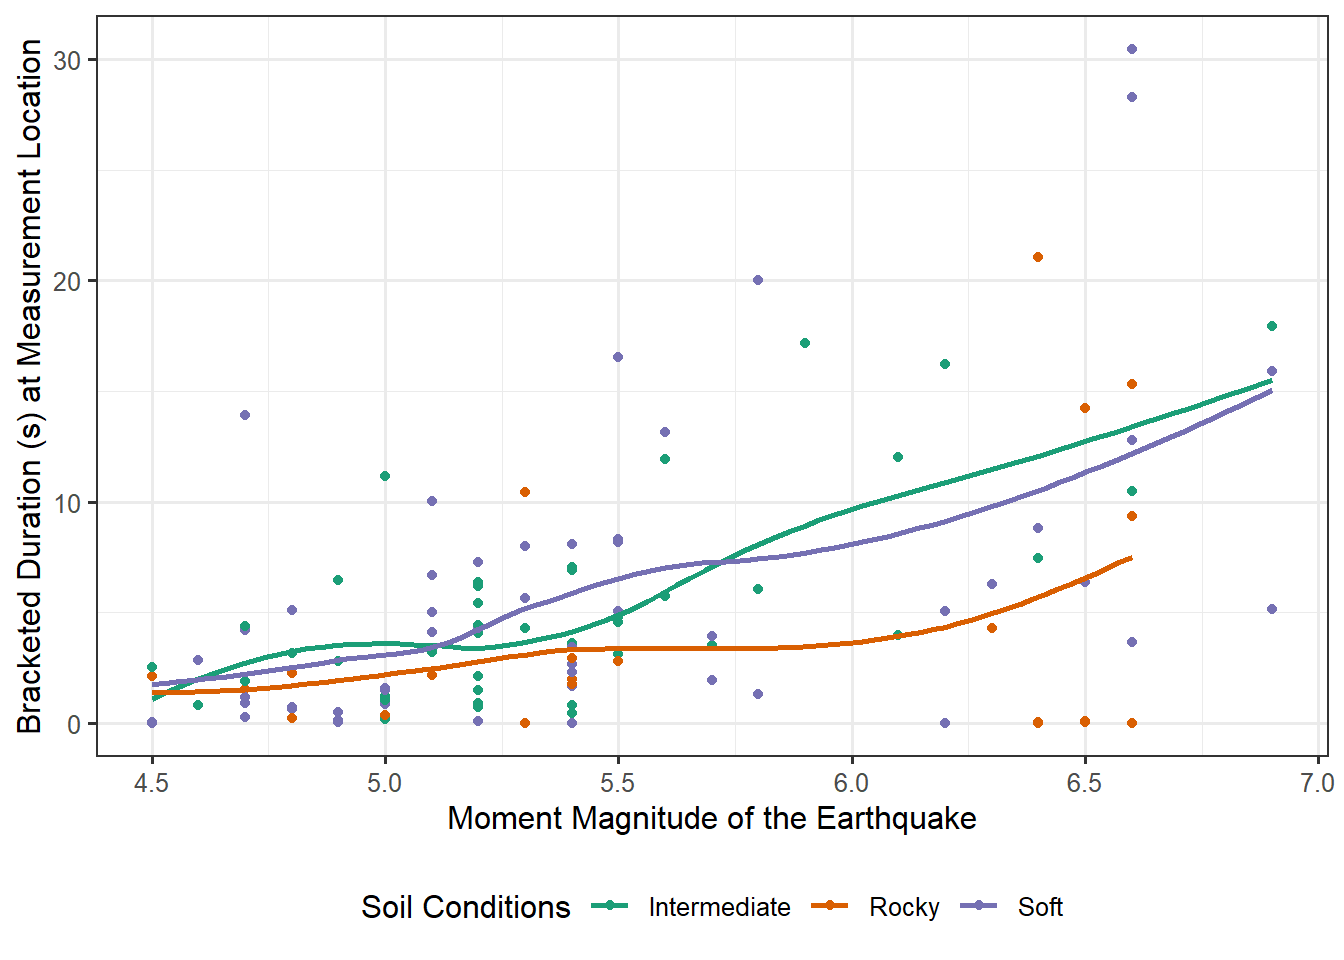
\includegraphics[width=0.8\linewidth]{./Images/regsummaries-color-1} 

}

\caption{Relationship of the bracketed duration and the magnitude of an earthquake with various soil conditions.}\label{fig:regsummaries-color}
\end{figure}

The figure illustrates that the relationship between magnitude and
bracketed duration is similar for both locations which have soft or
intermediate soil conditions. However, for rocky conditions, the
magnitude of the earthquake has a smaller impact on the resulting
bracketed duration. This suggests, possibly, that foundations on rocky
soils are less subject to the effects of an earthquake.

While our focus in this chapter has been on the scatter plot, our
emphasis remains the same as when we used simpler graphics in the first
unit --- summaries need to be constructed to address the question of
interest.

\chapter{Building our Statistical Model}\label{Regmodel}

In Chapter @ref(\#MeanModels) we introduced the statistical modeling
framework. In particular, our general model (see Equation
\eqref{eq:general-model}) was given as

\[\text{Response} = f(\text{variables, parameters}) + \text{noise}\] As
before, this model has two components:

\begin{itemize}
\tightlist
\item
  A deterministic component which takes the form of a function of
  variables and unknown parameters. It is often this component on which
  we would like to make inference.
\item
  A stochastic component which captures the unexplained variability in
  the data generating process.
\end{itemize}

In the previous unit, we made use of this model, but we only scratched
the surface of its potential applications. In this unit, we begin to
explore the full capabilities of such a model. In particular, we will
consider a model in which the deterministic component is a smooth
function (specifically, a line) of potentially several variables. In
general, this model building process is known as \textbf{regression}.

\BeginKnitrBlock{definition}[Regression]
\protect\hypertarget{def:defn-regression}{}{\label{def:defn-regression}
\iffalse (Regression) \fi{} }Used broadly, this refers to the process of
fitting a statistical model to data. More specifically, it is a process
of estimating the parameters in a data generating process.
\EndKnitrBlock{definition}

\section{Statistical Model for A Quantitative Response and Quantitative
Predictor}\label{statistical-model-for-a-quantitative-response-and-quantitative-predictor}

Recall that in Chapter \ref{MeanModels}, we described a general model
for the data generating process of a quantitative response:

\[\text{Response} = f(\text{predictor variables, parameters}) + \text{noise}\]

While Chapter \ref{MeanModels} focused on the function \(f(\cdot)\)
being a constant, this chapter considers alternative formulations. We
believe these models are best discussed in the context of the graphics
used to visualize them. Consider the
\protect\hyperlink{CaseGreece}{Seismic Activity Case Study}. Let's begin
with a broad question:

\begin{quote}
In general, does the bracketed duration increase as the magnitude
increases?
\end{quote}

As we are interested in predicting the bracketed duration, we will treat
it as the response. In order to imagine what an appropriate model might
look like, consider the graphical summary of this relationship. As we
have discussed, we can use a scatter plot to visualize the relationship
between the bracketed duration and the magnitude of the corresponding
earthquake. Figure \ref{fig:regmodel-slr-plot} gives the scatterplot but
also overlays a straight line relationship on top of the data.

\begin{figure}

{\centering 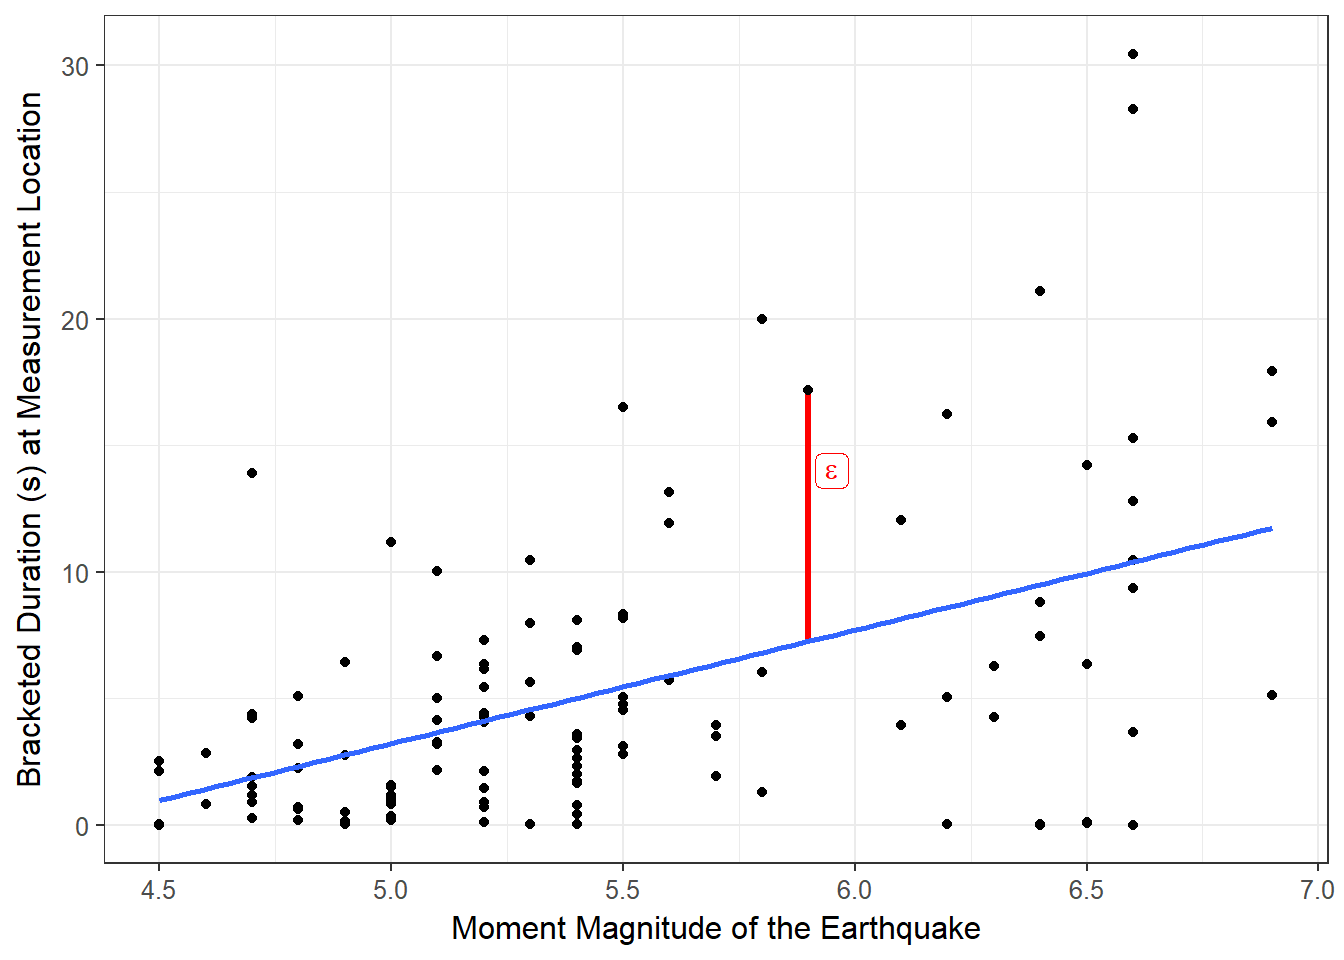
\includegraphics[width=0.8\linewidth]{./Images/regmodel-slr-plot-1} 

}

\caption{Relationship between bracketed duration and the magnitude of an earthquake with a line overlayed on the graphic as a potential explanation of the data generating process.}\label{fig:regmodel-slr-plot}
\end{figure}

Suppose we feel that this line is a good model for the data generating
process. Before proceeding, consider what this statement says. We are
not trying to say that the relationship explains every response we
observe. Instead, the relationship explains the underlying trend ---
what happens on average. While not perfect, this linear relationship at
least appears plausible. Therefore, we replace \(f(\cdot)\) in the
general form of a data generating process with a simple line, which we
express as

\begin{equation}
  (\text{Bracketed Duration})_i = \beta_0 + \beta_1(\text{Magnitude})_i + \epsilon_i
  \label{eq:regmodel-slr}
\end{equation}

where \(\beta_0\) represents the intercept of the line and \(\beta_1\)
the slope. Now, observe that very few points in Figure
\ref{fig:regmodel-slr-plot} actually fall on the line, which is to be
expected. This emphasizes the idea that the deterministic portion of the
model is not meant to fully capture a data generating process since
variability is inherent in any process. This is why statistical models
embed a deterministic component alongside a stochastic component --- to
capture the variability due to error or noise in the data generating
process.

The model suggests that the bracketed duration at a location is
primarily determined by the magnitude of the correpsonding event;
however, there is a component we cannot explain. That is, the model does
not explain why, for example, when an earthquake with a magnitude of 5.5
hits, all locations do not have the same bracketed duration. This noise
is picked up by the \(\epsilon_i\) term in the model (as illustrated in
red on Figure \ref{fig:regmodel-slr-plot}). The model essentially says
that the bracketed duration for a specific magnitude are simply
scattered vertically about the line. As we saw in Chapter
\ref{MeanModels}, we refine this model further by placing additional
conditions on the noise term in order to aid in conducting inference.

\BeginKnitrBlock{rmdtip}
For a quantitative response and quantitative predictor, the general form
of a simple linear regression model is then

\[(\text{Response})_i = \beta_0 + \beta_1(\text{Predictor})_i + \epsilon_i\]
\EndKnitrBlock{rmdtip}

\section{Using a Categorical
Predictor}\label{using-a-categorical-predictor}

We have described the simple linear model in this chapter as one which
relates two quantitative variables. However, this framework can be
extended to make use of a categorical predictor. For example, we saw in
Chapter \ref{Regsummaries} that the bracketed duration for locations
with rocky soils could differ from that of locations with other types of
soil. How do we include whether a location has rocky soil or not when
this is a categorical variable? The key is to construct an
\textbf{indicator variable}.

\BeginKnitrBlock{definition}[Indicator Variable]
\protect\hypertarget{def:defn-indicator-variable}{}{\label{def:defn-indicator-variable}
\iffalse (Indicator Variable) \fi{} }A binary variable (one which takes
on a value of 0 or 1) used to represent whether the value for a
categorical variable for an observation takes a particular value.
\EndKnitrBlock{definition}

Indicator variables essentially create a numeric variable which
represents a yes/no decision regarding a categorical variable. For
example, consider the following variable definition:

\[
(\text{Rocky Soil})_i = \begin{cases} 1 & \text{if } i\text{-th location has rocky soil} \\
0 & \text{if } i\text{-th location has a different soil type} \end{cases}
\]

We can then use this variable in our model for the data generating
process. Specifically, consider the following model

\begin{equation}
  (\text{Bracketed Duration})_i = \beta_0 + \beta_1(\text{Rocky Soil})_i + \epsilon_i  
  \label{eq:regmodel-ind}
\end{equation}

You may at first feel the need to have another indicator that takes the
value 1 when the soil is not rocky. But, this is not necessary. Think of
an indicator variable like a ``light switch.'' The indicator variable
turns on when an observation falls into a particular group and turns off
otherwise. So, if you have a location which has ``Intermediate'' soil
conditions, then that location cannot have ``Rocky'' soil, turning the
indicator off. Setting the indicator to 0 (turning it ``off'') then
leaves only the intercept in the model. So, the group which has a 0 for
the indicator is encoded in the intercept; this is known as the
\textbf{reference group}.

\BeginKnitrBlock{definition}[Reference Group]
\protect\hypertarget{def:defn-reference-group}{}{\label{def:defn-reference-group}
\iffalse (Reference Group) \fi{} }The group defined by setting all
indicator variables in a model to 0.
\EndKnitrBlock{definition}

The indicator variable essentially creates two mean responses, one for
each value of the indicator.For the model in Equation
\eqref{eq:regmodel-ind}, we have the following:

\[
\begin{aligned}
  \text{Rocky Soil:} &\quad (\text{Bracketed Duration})_i = \beta_0 + \beta_1 + \epsilon_i\\
  \text{Intermediate/Soft Soil:} &\quad (\text{Bracketed Duration})_i = \beta_0 + \epsilon_i
\end{aligned}
\]

So, the ``slope'' \(\beta_1\) is really capturing the shift in the
deterministic portion of the model from one group to the other. This is
illustrated in Figure \ref{fig:regmodel-ind-plot}. The ``line'' is
really connecting the location of the two groups.

\begin{figure}

{\centering 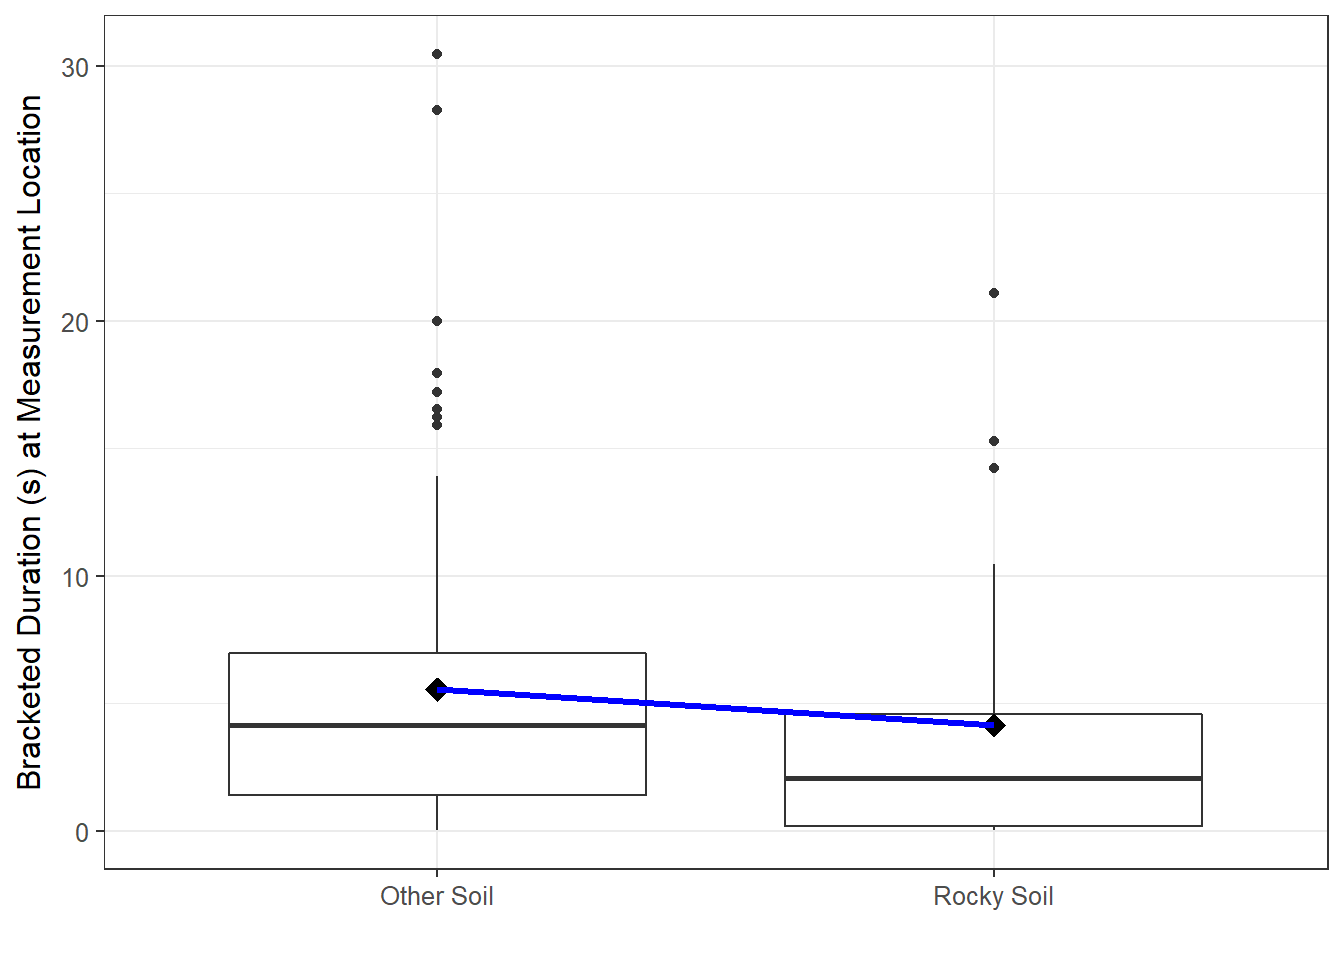
\includegraphics[width=0.8\linewidth]{./Images/regmodel-ind-plot-1} 

}

\caption{Comparison of the bracketed duration between locations with rocky soil and those with other soil types.}\label{fig:regmodel-ind-plot}
\end{figure}

\section{Estimating the Parameters}\label{estimating-the-parameters}

Recall the goal of statistics --- to use a sample to say something about
the underlying population. There is something intuitive about using the
sample mean as an estimate of the population mean; however, now we have
a model with both a slope and an intercept and we want to use the data
to say something about these parameters. That process begins by
computing an estimate for each of those parameters.

Before describing how such estimates are constructed, let us revisit the
model in Equation \eqref{eq:regmodel-slr}. In this equation, both
\(\beta_0\) and \(\beta_1\) are parameters and are therefore unknown
values, and they will always be unknown. We can use available data to
estimate these parameters with confidence (confidence intervals) or
determine if there is evidence they are outside of a specific region
(hypothesis testing), but we will never be able to definitively state
the value of these parameters. As scientists and engineers, many are
undoubtedly familiar with a line of ``best fit.'' We need to keep in
mind that any such line is simply an \emph{estimate}; no analysis can
actually provide the exact values of \(\beta_0\) and \(\beta_1\). But,
how are such estimates constructed?

Think about what we would like to do. We believe there is a linear
relationship which generated the data, and we want to use the data to
estimate what that relationship looks like. We want to draw a line
through the points that gives the ``best fit.'' Figure
\ref{fig:regmodel-least-squares} illustrates this for a hypothetical
dataset; it compares two \emph{estimated relationships}. We note that
these are just estimates; neither represents the actual line from which
the data was generated. Something inside us knows that the blue line is
preferred to the orange line. The orange line does not seem to represent
the pattern in the data because it leaves the cloud of points. We want a
line that goes through the points. Trying to formalize this, we are
saying we want a line that is somehow simultaneously as close to all the
data as possible.

\begin{figure}

{\centering 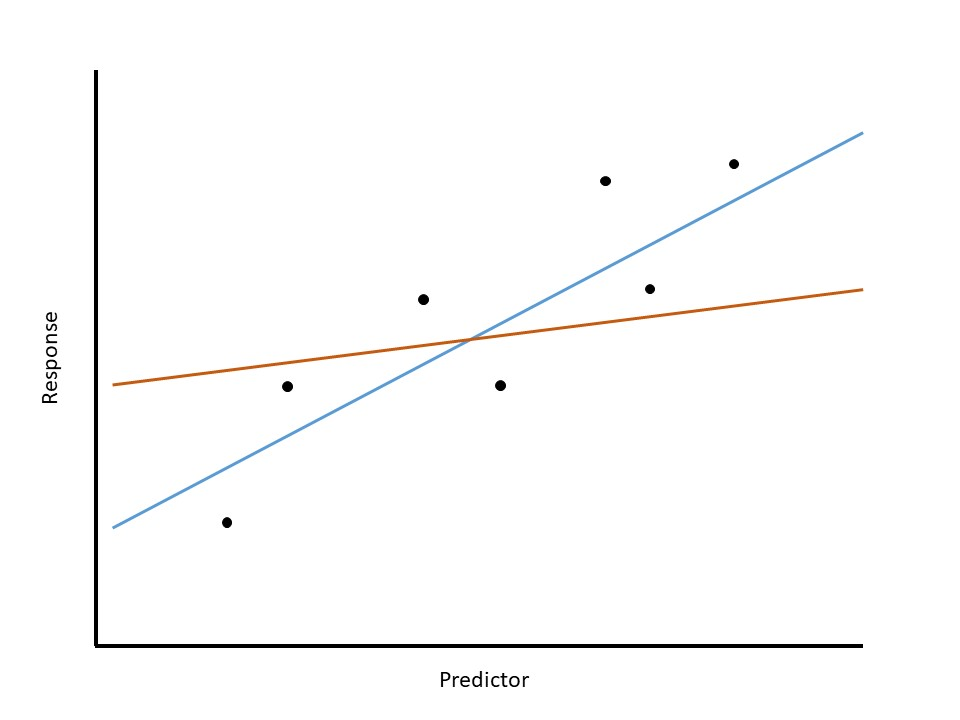
\includegraphics[width=0.8\linewidth]{./images/RegModel-LeastSquares} 

}

\caption{Illustration of two competing estimates of a line which runs through the data.}\label{fig:regmodel-least-squares}
\end{figure}

The most widely used method for estimating the parameters is known as
``the method of least squares.'' For this reason, the estimates are
often referred to as the \textbf{least squares estimates}. This method
essentially minimizes the amount of error (as measured by the vertical
distance a point is from the line) within the dataset.

\BeginKnitrBlock{definition}[Least Squares Estimates]
\protect\hypertarget{def:defn-least-squares-estimates}{}{\label{def:defn-least-squares-estimates}
\iffalse (Least Squares Estimates) \fi{} }Often called the ``best fit
line,'' these are the estimates of the parameters in a regression model
chosen to minimize the sum of squared errors. Formally, they are the
values of \(\beta_0\) and \(\beta_1\) which minimize the quantity

\[\sum_{i=1}^n \left((\text{Response})_i - \beta_0 - \beta_1(\text{Predictor})_{i}\right)^2\]

These estimates are often denoted
\(\widehat{\beta}_0, \widehat{\beta}_1\).
\EndKnitrBlock{definition}

This estimation is carried out using statistical software.

Estimation is often associated with statistics. However, the least
squares estimates are actually the result of a mathematical minimization
process. The real statistical aspect comes in when we move back into one
of our components of the \emph{Distributional Quartet}. In particular,
the estimates are only useful if we can quantify the variability in
those estimates. In order to construct a model for the sampling
distribution of these statistics, we place additional conditions on the
stochastic portion of the model. That is the focus of the next chapter.

\chapter{Conditions on the Error Term of a Regression
Model}\label{Regconditions}

In the previous chapter we developed a general model for generating a
quantitative response as a linear function of a quantitative predictor:

\[(\text{Response})_i = \beta_0 + \beta_1 (\text{Predictor})_{i} + \epsilon_i\]

We also discussed a common method for estimating the parameters of this
model from a sample --- the least squares method. However, if we are to
construct a model for the sampling distribution of these estimates we
must add some structure to the stochastic component \(\epsilon\) in the
model. We will find that the more assumptions we are willing to make,
the easier the analysis, but the less likely our model is to be
applicable to the actual data-generating process we have observed. The
conditions we make dictate how we conduct inference (the computation of
a p-value or confidence interval).

\section{Correctly Specified Model}\label{correctly-specified-model}

The first condition we consider is the most important. It states that
for every value of the predictor, the average error is 0. This condition
implies that the model we have posited for the data generating process
is accurate; that is, it implies that the form of the model is
appropriate --- that the response is linearly related to the predictor.
There are two reasons we say that this is the most important condition:

\begin{enumerate}
\def\labelenumi{\arabic{enumi}.}
\tightlist
\item
  If this condition is violated, it says your model for the data
  generating process is incorrect. Generally this is the result of
  ignoring some curvature or additional feature.
\item
  This condition allows us to interpret the parameters of the model.
\end{enumerate}

\subsection{Interpreting the
Parameters}\label{interpreting-the-parameters}

In the second unit, we were were focused on the mean response. Now,
instead of considering the average response overall, we are asking what
the average response is for subjects in the population with a specific
value of the predictor(s). When we impose the ``mean 0 condition,'' we
are saying the errors are not biasing the average response (since on
average, they have a value of 0); therefore, we are able to say that the
determinisic portion of our model is giving the \emph{average} response
for a specified value of the predictor(s).

\BeginKnitrBlock{rmdkeyidea}
The deterministic portion of a regression model specifies the
\emph{average} value of the response given the value(s) of the
predictor(s).
\EndKnitrBlock{rmdkeyidea}

As an example, consider our model for the
\protect\hyperlink{CaseGreece}{Seismic Activity Case Study} which
predicted the bracketed duration as a function of the magnitude of the
earthquake:

\[(\text{Bracketed Duration})_i = \beta_0 + \beta_1(\text{Magnitude})_i + \epsilon_i\]

When the errors have mean 0 for all magnitudes (our first condition),
then earthquakes with a 5.0 magnitude have an \emph{average} bracketed
duration of

\[\beta_0 + \beta_1(5)\]

Similarly, earthquakes with a 6.0 magnitude have an \emph{average}
bracketed duration of

\[\beta_0 + \beta_1(6)\]

As we have mentioned, the deterministic portion of the model does not
specify the exact response for any individual but the trend. We are now
able to say that the ``trend'' we are modeling is the average response.
Further, we can estimate this average response by plugging in the least
squares estimates \(\widehat{\beta}_0\) and \(\widehat{\beta}_1\).
Specifically, using the method of least squares, the line of best fit
was estimated as

\[(\text{Bracketed Duration}) = -19.19 + 4.48 (\text{Magnitude})\]

Therefore, we estimate the average bracketed duration for locations with
5.0 magnitude earthquakes to be 3.22 seconds (7.71 seconds for locations
with 6.0 magnitude earthquakes). While we do not expect every location
which has a 5.0 magnitude earthquake to have a bracketed duration of
this length, we expect the bracketed duration to vary about this length
of time. This is huge; it says that when we use a regression model to
predict a response, we are actually predicting the \emph{average}
response. More, we can interpret the parameters themselves.

Let's begin with the intercept term, \(\beta_0\). Notice that in our
model above, if we try to predict the bracketed duration for a location
with an earthquake which has a magnitude of 0, then our model returns
\(\beta_0\). In fact, for any regression model, the intercept
\(\beta_0\) is the value of the deterministic portion of the model
whenever all predictors in the model are set to 0. And, that
deterministic portion is the average response.

\BeginKnitrBlock{rmdtip}
The intercept in a regression model \(\beta_0\) represents the
\emph{average} response when all predictors in the model are set equal
to 0. Note that this may not be practically meaningful in all contexts.
\EndKnitrBlock{rmdtip}

For our particular example, the estimate of the intercept does not make
sense --- what does it mean to have a duration of -19.19 seconds? More,
it does not make sense to estimate the average bracketed duration for an
earthquake which had a magnitude of 0 (not even an earthquake). This can
often be the case when trying to interpret the intercept term due to
what we call \textbf{extrapolation}. We do not have any data on the
bracketed duration for locations which experienced an earthquake with a
magnitude less than 4.5. Therefore, we are using a model to predict for
a region over which the model was not constructed to operate. This is a
lot like using a screw driver to hammer a nail --- we are using a tool
to accomplish a task for which it was not designed. We should not be
surprised when it fails. The primary reason extrapolation is dangerous
is that without data in a particular region, we have nothing supporting
that the model will continue to hold in that region. We have illustrated
this when discussing the intercept, but extrapolation can occur in any
region for which there is no data. For this reason, unless you have
strong scientific justification for why a model will hold over all
values of the predictor, extrapolation should be avoided

\BeginKnitrBlock{definition}[Extrapolation]
\protect\hypertarget{def:defn-extrapolation}{}{\label{def:defn-extrapolation}
\iffalse (Extrapolation) \fi{} }Using a model to predict outside of a
region for which data is available.
\EndKnitrBlock{definition}

We have seen that the intercept is the average value of the response
when the predictor has the value of 0. How then do we interpret the
coefficient associated with the predictor (the slope). We again use an
example. Notice that based on our estimates, the average bracketed
duration is 4.48 seconds longer for those locations which experience a
6.0 magnitude earthquake compared to those which experience a 5.0
magnitude earthquake, and this difference is the value of the estimated
slope. This leads us to observing that 4.48 seconds is the change in the
average bracketed duration that is associated with a 1-unit increase in
the magnitude of an earthquake.

\BeginKnitrBlock{rmdtip}
The coefficient (or slope) \(\beta_1\) in a regression model represents
the \emph{average} change in the response associated with a 1 unit
\emph{increase} in the predictor.
\EndKnitrBlock{rmdtip}

\subsection{Embedding our Question in a Statistical
Framework}\label{embedding-our-question-in-a-statistical-framework}

Our first fundamental idea centers on the idea that the majority of
research questions can be framed in terms of a parameter within the
population. This seemed somewhat intuitive when the parameter was simply
the mean response. With parameters which are the slope and intercept of
a line, this seems less clear. However, this condition that the errors
have mean 0 for all values of the predictor (because of its implications
on the interpretation of the parameters) ensures that our questions of
interest can be framed in terms of the parameters. Consider the
following question:

\begin{quote}
On average, is the bracketed duration related to the magnitude of an
earthquake?
\end{quote}

Let's consider how we might write this in terms of a null and
alternative hypotheses.

\begin{quote}
\(H_0:\) the bracketed duration does not change, on average, as the
magnitude changes.\\
\(H_1:\) the bracketed duration is linearly related, on average, with
the magnitude; that is, as the magnitude increases, the bracketed
duration changes, on average.
\end{quote}

In order to address this question, we considered the following model for
the data generating process:

\[(\text{Bracketed Duration})_i = \beta_0 + \beta_1(\text{Magnitude})_i + \epsilon_i\]

If the null hypothesis above is true, then that suggests that the
bracketed duration is flat on average, regardless of the value of the
magnitude. What would be true about the parameters if that were true?
Remember that \(\beta_1\) captures the change in the average bracketed
duration as the magnitude increases by 1 unit; and, the null hypothesis
says that there is no change in the average bracketed duration as the
magnitude changes. That is, if the null hypothesis is true,
\(\beta_1 = 0\). Said another way, we need a model for which changing
the value of the magnitude does not affect the resulting bracketed
duration --- a flat line. Therefore, our null and alternative hypotheses
can be written as

\begin{quote}
\(H_0: \beta_1 = 0\)\\
\(H_1: \beta_1 \neq 0\)
\end{quote}

where \(\beta_1\) is the parameter linearly relating the bracketed
duration to the magnitude. That is, if the paramter associated with
magnitude is 0, then it is plays no role in the data generating process;
if it is anything other than 0, then magnitude has a role within the
data generating process.

\BeginKnitrBlock{rmdkeyidea}
Setting a slope parameter to 0 in the model for a data generating
process is associated with saying that the corresponding predictor is
not associated with the response in a linear fashion --- that it does
not belong in the model.
\EndKnitrBlock{rmdkeyidea}

The interpretation of our parameters allows us to see that our research
questions are characterizing the relationship between the response and
the predictor, \emph{on average}. As in the previous unit, our questions
are about the average response; instead of looking at the overall
average, however, we are allowing it to depend upon a predictor.

This first condition on the error term --- holding the average error to
be 0 for all values of the predictor --- is only one condition typically
placed on the stochastic portion. We now desribe others.

\section{Additional Conditions}\label{additional-conditions}

The second condition we consider is that the noise attributed to one
observed individual is independent of the noise attributed to any other
individual observed. That is, the amount of error in any one
individual's response is unrelated to the error in any other response
observed. This is the same condition we introduced in Chapter
\ref{MeanModels}. We still want each observation in our data to be
independent of one another.

With just these first two conditions (that the average error is 0 for
all values of the predictors and the errors are independent of one
another), we can use a bootstrap algorithm in order to model the
sampling distribution of the least squares estimate for the slope (as
well as the intercept). However, additional conditions are often placed
on the error term.

The third condition that is typically placed on the distribution of the
errors is that the errors are identically distributed. Again, we
introduced this condition in Chapter \ref{MeanModels}. However, in the
context of regression, this is often described a bit differently. In
particular, if the errors are not identically distributed, it is
typically because the variability of the error differs for one value of
the predictor compared to another. Practically, this reveals itself as
our response being more precise in one region than in another. As a
result of focusing on the variability of the response for each
predictor, this condition is often referred to as
\emph{homoskedasticity} instead of the errors being identically
distributed.

With this additional condition imposed, we are able to modify our
bootstrap algorithm when constructing a model for the sampling
distribution of the least squares estimates. Because we are relying on a
bootstrap procedure, our model for the sampling distribution or null
distribution, depending on whether we are interested in computing a
confidence interval or p-value) is empirical. As a result, our model for
the sampling distribution can be unstable in small sample sizes; this
can be avoided by building an analytical model for the sampling
distribution. This requires us to impose a fourth condition (common in
the engineering and science disciplines) on the distribution of the
errors and then rely on some probability theory.

\subsection{Modeling the Population}\label{modeling-the-population}

Before we delve into more detail, let's set the stage for the bigger
story being told. Recall that our goal is to say something about the
population using a sample. We have developed a process to address this
goal:

\begin{enumerate}
\def\labelenumi{\arabic{enumi}.}
\tightlist
\item
  Frame our question through a parameter of interest.
\item
  Collect data that allows us to estimate the parameter using the
  analogous statistic within the sample.
\item
  Summarize the variability in the data graphically.
\item
  Quantify the variability in the statistic through modeling the
  sampling distribution (or null distribution, whichever is
  appropriate).
\item
  Using the sampling distribution , quantify the evidence in the sample.
\end{enumerate}

This process is presented through our \emph{Five Fundamental Ideas of
Inference} and the \emph{Distributional Quartet}. The key step in this
process is quantifying the variability by modeling the \emph{sampling
distribution} (or \emph{null distribution}, whichever is appropriate for
our research goal). We have described the construction of these models
empirically, through repeating the study by appropriately resampling the
data available and performing the analysis on each resample.

Our goal is still to model the sampling distribution; that is the key
inferential step. Instead of building an empirical model, we can
construct an exact analytical model through an additional step: modeling
the population directly.

\BeginKnitrBlock{rmdkeyidea}
A model for the sampling distribution of a statistic can often be
obtained by placing a model on the distribution of the population.
\EndKnitrBlock{rmdkeyidea}

So, we have two distributional models; the model for the distribution of
the population is simply a stepping stone to a model for the sampling
distribution of the statistic, which is what we really need. It is
important to separate these steps. We are not interested in directly
modeling the population; we do it in order to construct a model for the
sampling distribution.

There is one other distinction to make: a model for the population is
\emph{always} an assumption. We hope that the data is consistent with
this assumption in order to apply the resulting model for the sampling
distribution. In later chapters, we will discuss how we assess whether
our data is consistent with these conditions; for now, we simiply want
to understand we are making an assumption when we place such a condition
on the stochastic portion of data generating process.

\section{Adding the Assumption of
Normality}\label{adding-the-assumption-of-normality}

Probability, a sub-field of mathematics which is used heavily in
statistics, is the discipline of modeling randomness. In particular, we
make use of probability to model a distribution. In order to get a feel
for probability models, consider the following example.

\BeginKnitrBlock{example}[Iris Characteristics]
\protect\hypertarget{exm:ex-iris}{}{\label{exm:ex-iris} \iffalse (Iris
Characteristics) \fi{} }The discipline of statistics began in the early
1900's primarily within the context of agricultural research. Edgar
Anderson was a researcher investigating the characteristics of the iris.
He had collected measurements on over one hundred iris flowers,
including their petal length and width and their sepal length and width.
The sepal is the area (typically green) beneath the petal of a flower.
It offers protection while the flower is budding and then support for
the petals after the flower blooms.
\EndKnitrBlock{example}

Figure \ref{fig:regconditions-iris-histogram} is a histogram of the
sepal width for the iris plants observed by Edgar Anderson; overlayed is
the density plot for the same dataset, which we have described as a
smoothed histogram. Both the histogram and the density plot are
empirical models of the distribution of the sepal width.

\begin{figure}

{\centering 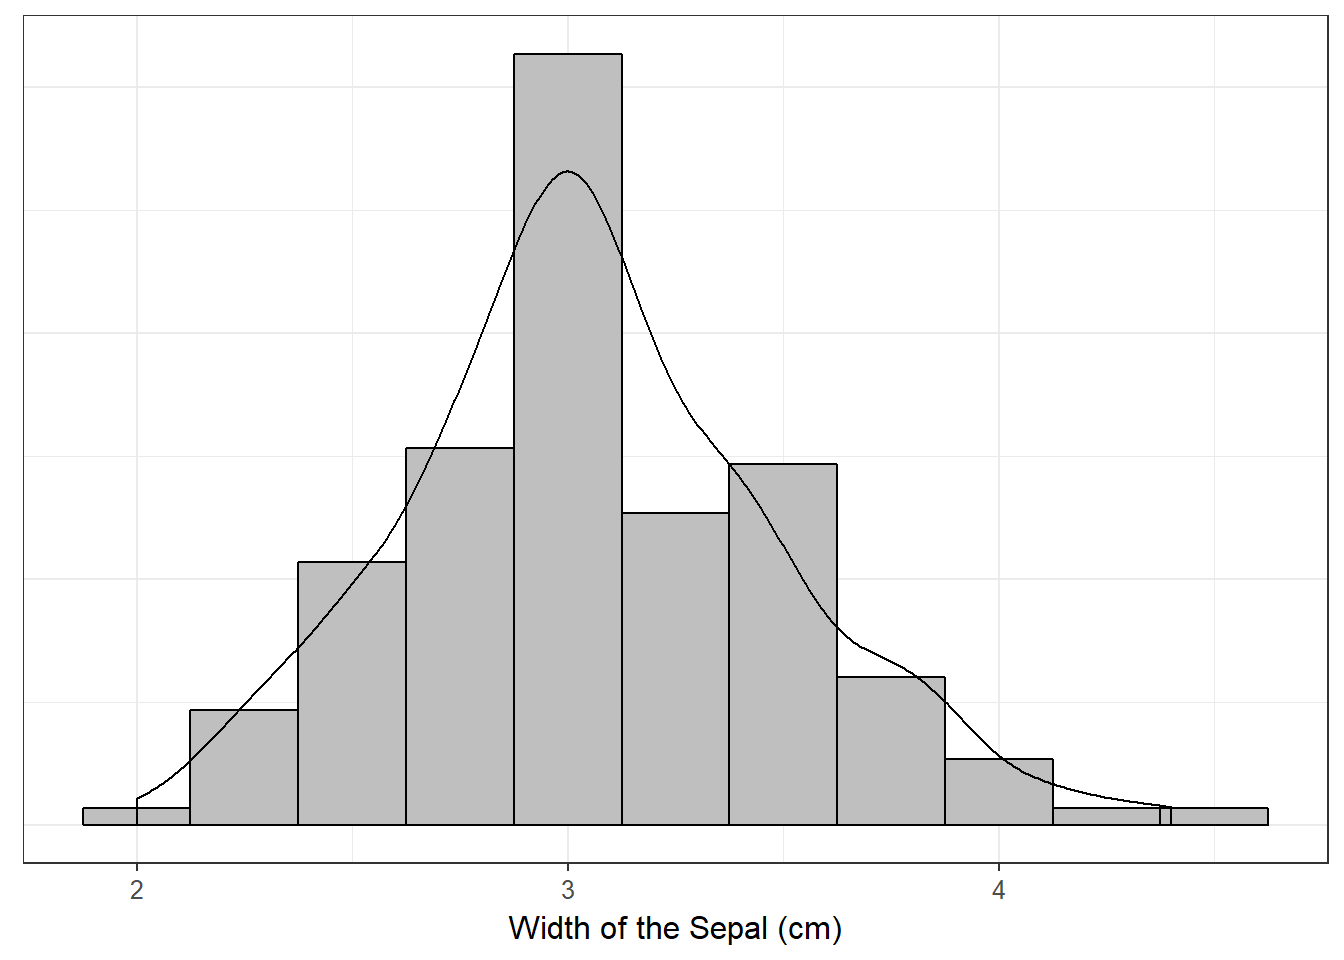
\includegraphics[width=0.8\linewidth]{./Images/regconditions-iris-histogram-1} 

}

\caption{Summary of the distribution of sepal widths for a sample of irises.}\label{fig:regconditions-iris-histogram}
\end{figure}

Probability models are analytical models for the distribution of a
variable. Instead of constructing a density using data, probability
theory posits a functional form for the density. For example, Figure
\ref{fig:regconditions-iris-normal} overlays the following function on
top of the the iris data:

\[f(x) = \frac{1}{\sqrt{0.380\pi}} e^{-\frac{1}{0.380}(x - 3.057)^2}\]

\begin{figure}

{\centering 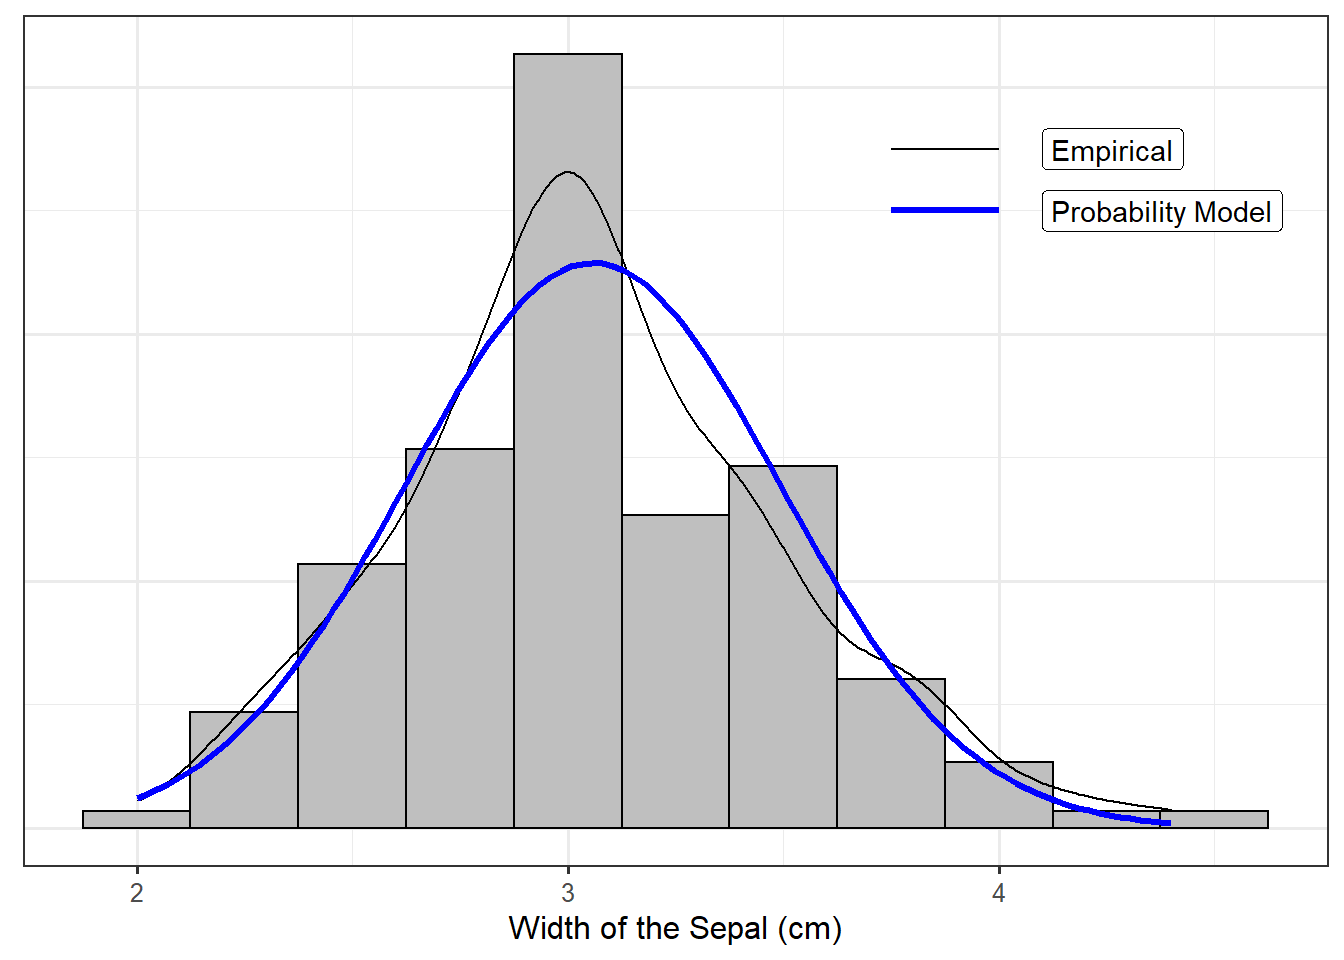
\includegraphics[width=0.8\linewidth]{./Images/regconditions-iris-normal-1} 

}

\caption{Summary of the distribution of the sepal widths for a sample of irises with a probability model overlayed.}\label{fig:regconditions-iris-normal}
\end{figure}

A density (whether constructed empirically or posited analytically) is
just a model for the distribution of a variable. Further, all density
functions share a few basic properties:

\begin{enumerate}
\def\labelenumi{\arabic{enumi}.}
\tightlist
\item
  The density is non-negative for all values of the variable.
\item
  The area under the density function must equal 1.
\end{enumerate}

While the value on the y-axis is not directly meaningful, density
functions provide a link between the value of the variable and the
likelihood of it occuring. Specifically, the probability that a variable
falls in a specific range corresponds to the area under the curve in
that region. For example, based on the analytical model described above
(the blue curve in the figure), the probability that an iris has a sepal
width between 3.5 and 4 centimeters is 0.14, illustrated in Figure
\ref{fig:regconditions-iris-prob}. That is, there is a 14\% chance we
find an irish with a sepal width between 3.5 and 4 centimeters.

\begin{figure}

{\centering 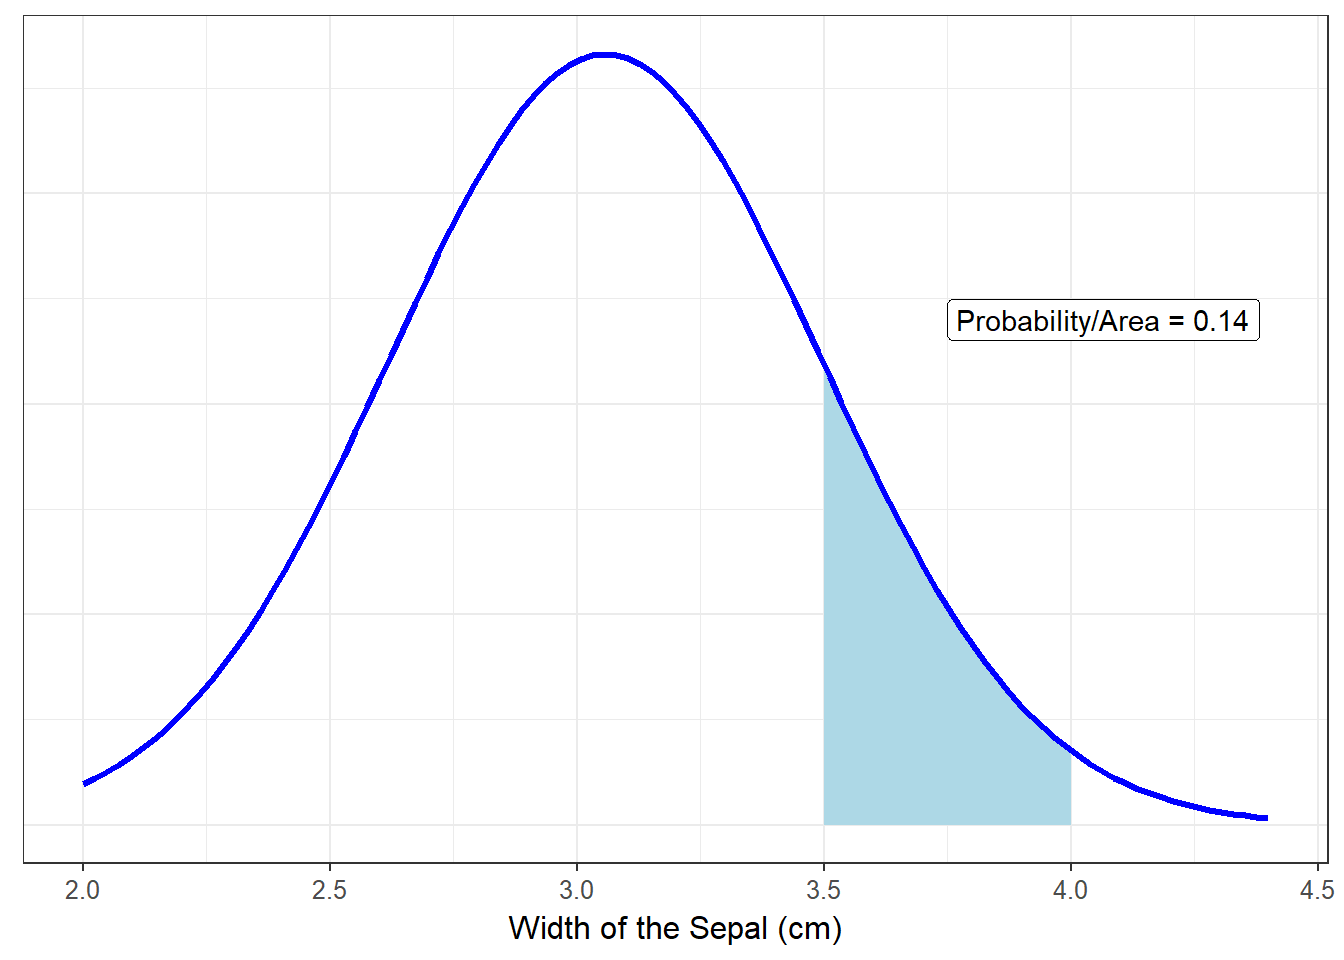
\includegraphics[width=0.8\linewidth]{./Images/regconditions-iris-prob-1} 

}

\caption{Using the model for a density function to compute a probability.}\label{fig:regconditions-iris-prob}
\end{figure}

While the above model for the density is not perfect, it does capture
many of the characteristics present in the data. Similar to empirical
models, analytical models for distributions are just that ---
\emph{models}. This particular model, characterized by the bell-shape
density, is known as the \textbf{Normal Distribution}.

\BeginKnitrBlock{definition}[Normal Distribution]
\protect\hypertarget{def:defn-normal-distribution}{}{\label{def:defn-normal-distribution}
\iffalse (Normal Distribution) \fi{} }Also called the Gaussian
Distribution, this probability model is popular for modeling noise
within a data-generating process. It has the following characteristics:

\begin{itemize}
\tightlist
\item
  It is bell-shaped.
\item
  It is symmetric, meaning the mean is directly at its center, and the
  lower half of the distribution looks like a mirror image of the upper
  half of the distribution.
\item
  Often useful for modeling natural phenomena or sums of measurements.
\end{itemize}

The functional form of the Normal distribution is
\[f(x) = \frac{1}{\sqrt{2\pi\sigma^2}} e^{-\frac{1}{2\sigma^2}(x - \mu)^2}\]

where \(\mu\) is the mean of the distribution and \(\sigma^2\) is the
variance of the distribution.
\EndKnitrBlock{definition}

While there are several nice properties of the Normal Distribution, we
are primarily interested in the fact that if the error in a data
generating process follows a Normal Distribution (in addition to the
other three conditions described above placed on the error term), then
the form of the sampling distribution for the least squares estimates of
the slope and intercept is known. That is, with all four conditions in
place, we have an analytical model for the sampling distribution. This
means we avoid simulating in order to build a model for the sampling
distribution; so, computationally it is faster. If the errors really are
from a Normal Distribution, then we also gain power in our study by
imposing this condition. Finally, such a model does not rely on
sufficient data to construct; it is valid for any sample size (of
course, large samples will always decrease variability in the estimates,
which is a plus).

Let's think about what this condition means for the responses. Given the
shape of the Normal distribution, imposing this condition (in addition
to the other conditions) implies that some errors are positive and some
are negative. This in turn implies that some responses will tend to fall
above the line (we will underpredict for these observations), and some
response will tend to fall below the line (we will overpredict for these
observations).

\section{Classical Regression Model}\label{classical-regression-model}

We have discussed four conditions we could place on the stochastic
portion of the data generating process. Placing all four conditions on
the error term is what we refer to as the ``Classical Regression
Model.''

\BeginKnitrBlock{definition}[Classical Regression Model]
\protect\hypertarget{def:defn-classical-regression}{}{\label{def:defn-classical-regression}
\iffalse (Classical Regression Model) \fi{} }For a quantitative response
and single predictor, the classical regression model assumes the
following data-generating process:

\[(\text{Response})_i = \beta_0 + \beta_1 (\text{Predictor})_{i} + \epsilon_i\]

where

\begin{enumerate}
\def\labelenumi{\arabic{enumi}.}
\tightlist
\item
  The error in the response has a mean of 0 for all values of the
  predictor.
\item
  The error in the response for one subject is independent of the error
  in the response for all other subjects.
\item
  The errors are identically distributed for all values of the
  predictor. This is often stated as the variability in the error of the
  response is the same for all values of the predictor.
\item
  The errors follow a Normal Distribution.
\end{enumerate}

This is the default ``regression'' analysis implemented in the majority
of statistical packages.
\EndKnitrBlock{definition}

We note that regression need not require these conditions. Placing all
four conditions on the error term results in a specific analytical model
for the sampling distribution of the least squares estimates. Changing
the conditions changes the way we model the sampling distribution.

\BeginKnitrBlock{rmdkeyidea}
The model for the sampling distribution of a statistic is determined by
the conditions you place on the data generating process.
\EndKnitrBlock{rmdkeyidea}

We have stressed the implications of each condition individually. Figure
\ref{fig:regconditions-assumptions} illustrates these conditions working
together. The condition that the errors have mean 0 implies that for a
given value of the predictor, the average response is given by the line
(shown as the green dot in the figure). The condition of Normality
implies that for a given value of the predictor, the response is
distributed evenly about the regression line, with some above and some
below. Further, the shape of the Normal distribution implies that these
responses will cluster about the line. The identically distributed
condition (specifically homoskedasticity) implies that while the
responses vary around the line, they do so the same degree, regardless
of the value of the predictor. Therefore, the model is just as precise
for all values of the predictor. Finally, any two responses must be
unrelated.

\begin{figure}

{\centering 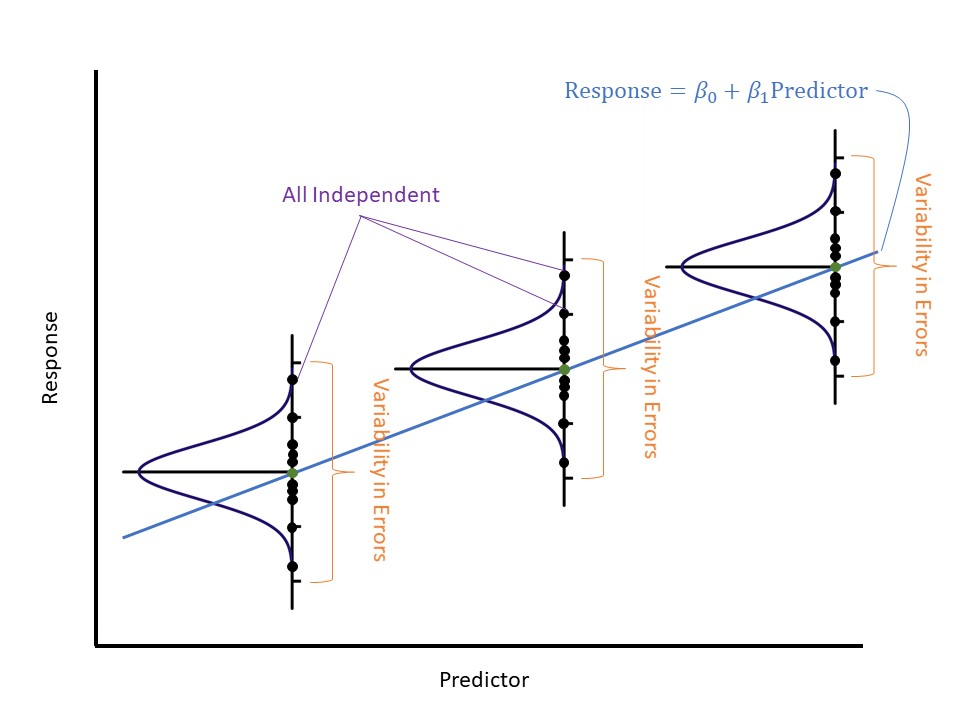
\includegraphics[width=0.8\linewidth]{./images/RegConditions-Assumptions} 

}

\caption{Illustration of the conditions on the error term for the classical regression model.}\label{fig:regconditions-assumptions}
\end{figure}

\section{Imposing the Conditions}\label{imposing-the-conditions}

Let's return to our model for the bracketed duration as a function of
the magnitude of the corresponding earthquake:

\[(\text{Bracketed Duration})_i = \beta_0 + \beta_1(\text{Magnitude})_i + \epsilon_i\]

Our hypotheses of interest which captures the question of interest was

\begin{quote}
\(H_0: \beta_1 = 0\)\\
\(H_0: \beta_1 \neq 0\)
\end{quote}

which corresponds to testing whether there is evidence of a linear
relationship between the two variables. Using the method of least
squares, we estimated the parameters in the model; this leads to the
following equation for estimating the average bracketed duration given
the magnitude:

\[(\text{Brackted Duration}) = -19.19 + 4.48(\text{Magnitude})\]

If we are willing to assume the data is consistent with the conditions
for the classical regression model, we are able to model the sampling
distribution of these estimates and therefore construct confidence
intervals. Table \ref{tab:regconditions-slr-summary} summarizes the fit
for the above model. In addition to the least squares estimates, it also
contains the \textbf{standard error} of the statistic, quantifying the
variability in the estimates.

\BeginKnitrBlock{definition}[Standard Error]
\protect\hypertarget{def:defn-standard-error}{}{\label{def:defn-standard-error}
\iffalse (Standard Error) \fi{} }The estimated standard deviation of a
statistic, computed from the model for the statistic's sampling
distribution. It quantifies the variability in the sampling distribution
of the statistic.
\EndKnitrBlock{definition}

Finally, there is a 95\% confidence interval estimating each parameter.
Notice that based on the confidence interval for the slope, 0 is not a
reasonable value for this parameter. Therefore, we have evidence that
the slope coefficient associated with the magnitude differs from 0; that
is, we have evidence of a linear relationship between the bracketed
duration and the magnitude of the earthquake.

\begin{table}

\caption{\label{tab:regconditions-slr-summary}Summary of the linear model fit relating the bracketed duration at locations in Greece following an earthquake with the magnitude of the event.}
\centering
\begin{tabular}[t]{l|r|r|r|r}
\hline
Term & Estimate & Standard Error & Lower 95\% CI & Upper 95\% CI\\
\hline
(Intercept) & -19.194 & 3.975 & -27.066 & -11.323\\
\hline
Magnitude & 4.484 & 0.724 & 3.050 & 5.917\\
\hline
\end{tabular}
\end{table}

We have described in general how confidence intervals are constructed.
Under the classical regression model, there is an analytical model for
the sampling distribution, and it is known. As a result, the confidence
interval can be computed from a formula.

\BeginKnitrBlock{rmdtip}
If the classical regression model is assumed, the 95\% confidence
interval for the parameter \(\beta_j\) can be approximated by

\[\widehat{\beta}_j \pm (1.96)\left(\text{standard error of } \widehat{\beta}_j\right)\]
\EndKnitrBlock{rmdtip}

The confidence interval for the change in the average bracketed duration
for each 1-unit increase in the magnitude of an earthquake (the slope
\(\beta_1\)) was constructed assuming the classical regression model.
Suppose, however, that we are only willing to impose the following
conditions:

\begin{itemize}
\tightlist
\item
  The error in the bracketed duration is 0 on average for earthquakes of
  any magnitude.
\item
  The error in the bracketed duration for one earthquake is independent
  of the error in the bracketed duration for any other earthquake.
\end{itemize}

Since the conditions have been altered, the model for the sampling
distribution of the estimates will change and therefore the
corresponding confidence intervals. Under these conditions, we can
appeal to a bootstrapping algorithm. Specifically, we could resample
(with replacement) 119 earthquakes from the original data; for each
resample, we compute the least squares fit (see Figure
\ref{fig:regconditions-bootstrap}). Since the observations selected
change with each resample, the least squares estimates will also change.
By repeating this process over and over again, we can obtain a model for
how the estimates would change in repeated sampling.

\begin{figure}

{\centering \includegraphics[width=0.8\linewidth]{./images/RegConditions-Bootstrap} 

}

\caption{Illustration of a single iteration of a bootstrap procedure to construct an empirical estimate of the sampling distribution for the estimates of the coefficients in a regression model.}\label{fig:regconditions-bootstrap}
\end{figure}

Using the empirical model of the sampling distribution for each
estimate, we can construct confidence intervals. These updated
confidence intervals are shown in Table
\ref{tab:regconditions-slr-summary-alt}

\begin{table}

\caption{\label{tab:regconditions-slr-summary-alt}Summary of the linear model fit relating the bracketed duration at locations in Greece following an earthquake with the magnitude of the event. Only assumes errors are independent and have mean 0.}
\centering
\begin{tabular}[t]{l|r|r|r|r}
\hline
Term & Estimate & Standard Error & Lower 95\% CI & Upper 95\% CI\\
\hline
(Intercept) & -19.194 & 4.960 & -29.258 & -9.545\\
\hline
Magnitude & 4.484 & 0.965 & 2.593 & 6.437\\
\hline
\end{tabular}
\end{table}

While the exact interval differs from what we computed previously, our
overall conclusion remains the same (there is evidence of a
relationship). It is reasonable to ask, which confidence interval should
we use? That depends on the conditions you are willing to assume, which
is an issue we will tackle soon.

\section{Recap}\label{recap}

We have covered a lot of ground in this chapter, and it is worth taking
a moment to summarize the big ideas. In order to construct a model for
the sampling distribution for the estimates of the parameters in the
regression model, we took a step back and modeled the data generating
process. Such a model consists of two components: a deterministic
component explaining the differences in the response as a function of
the predictor and a stochastic component capturing the noise in the
system.

Certain conditions are placed on the distribution of the noise in our
model. With a full set of conditions (classical regression model), we
are able to model the sampling distribution analytically. We can also
construct an empirical model for the sampling distribution assuming the
data is consistent with fewer conditions.

\chapter{Quantifying the Quality of a Model Fit}\label{Regquality}

In the previous two chapters, we described a model for describing the
data generating process for a quantitative response as a function of a
single quantitative predictor:

\[(\text{Response})_i = \beta_0 + \beta_1 (\text{Predictor})_i + \epsilon_i\]

We can obtain estimates of the unknown parameters in this model using
least squares. Further, under certain conditions on the error term, we
are able to construct valid confidence intervals for the parameters. We
have not yet discussed how to compute p-values to test hypotheses about
the parameters, nor have we discussed how to determine if our model is
useful for making predictions. It turns out these two tasks are very
much related and are accomplished through partitioning variability. Much
of statistics is about accounting for various sources of variability;
and, this process allows us to compare models for the data generating
process. In this chapter, we will describe what we mean by partitioning
variability and how it is used to derive a measure for the overall
performance of a model and to develop a standardized statistic for
comparing two models.

\section{Partitioning Variability}\label{partitioning-variability}

Consider modeling the bracketed duration as a function of the distance
the location is from the center of the earthquake:

\[(\text{Bracketed Duration})_i = \beta_0 + \beta_1(\text{Epicentral Distance})_i + \epsilon_i\]

Using least squares to estimate the parameters, and assuming the data is
consistent with the conditions for the classical regression model, the
resulting model fit is summarized below in Table
\ref{tab:regquality-fit}.

\begin{table}

\caption{\label{tab:regquality-fit}Summary of the model fit explaining the bracketed duration as a function of epicentral distance.}
\centering
\begin{tabular}[t]{l|r|r|r|r}
\hline
Term & Estimate & Standard Error & Lower 95\% CI & Upper 95\% CI\\
\hline
(Intercept) & 4.462 & 0.726 & 3.024 & 5.899\\
\hline
Epicentral Distance & 0.029 & 0.018 & -0.007 & 0.064\\
\hline
\end{tabular}
\end{table}

Remember, the goal of the model for the data generating process is to
explain why the response is the value we see --- we are essentially
explaining why the values of the response differ from one individual to
another (its variability). Consider the model for the data generating
process summarized above; it posits two reasons why the bracketed
duration is not the same value at each measured location:

\begin{itemize}
\tightlist
\item
  The locations are located different distances from the epicenter of
  each earthquake.
\item
  Additional noise due to measurement error in the bracketed duration or
  additional natural sources we are unable to explain.
\end{itemize}

Looking at the form of the model for the data generating process, it may
seem obvious that there are these two sources of variability --- two
sources for why the bracketed duration differs from one individual to
another. However, it is not yet clear how we quantify the amount of
variability in each. We want to quantify the amount of variability in
the response that can be attributed to each of these components. That
is, we move forward with a goal of trying to say something like

\[(\text{Total Variability in Bracketed Duration}) = (\text{Variability due to Distance}) + (\text{Variability due to Noise})\]

As we have seen in both Chapters \ref{Summaries} and
\ref{SingleTestStat}, variability can be quantified through considering
the ``total'' distance (squared) the observations are from a common
target (the mean response). That is, the total variability in bracketed
duration can be measured by

\[\sum_{i=1}^{n} \left((\text{Bracketed Duration})_i - (\text{Mean Bracketed Duration})\right)^2\]

Notice this quantity is similar to, but not exactly the sample variance.
It measures the distance each response is from the sample mean and then
adds these distances up. This is known as the \textbf{Total Sum of
Squares} since it captures the total variability in the response.

\BeginKnitrBlock{definition}[Total Sum of Squares]
\protect\hypertarget{def:defn-sst}{}{\label{def:defn-sst} \iffalse (Total
Sum of Squares) \fi{} }Let \(y_i\) denote the response for the \(i\)-th
observation and \(\bar{y}\) denote the sample mean response. Then, the
Total Sum of Squares (abbreviated SST) is given by

\[SST = \sum_{i=1}^{n} \left(y_i - \bar{y}\right)^2\]
\EndKnitrBlock{definition}

We now have a way of quantifying the total variability in bracketed
duration; we now want to quantify its two components specified by the
model (variability due to epicentral distance and variability due to
noise). In order to capture the variability due epicentral distance, we
consider how epicentral distance plays a role in the model for the data
generating process: it forms the line which dictates the mean response.
That is, the linear portion in the model
\(\beta_0 + \beta_1 (\text{Epicentral Distance})\) is the model's
attempt to explain how epicentral distance explains the bracketed
duration; further, this explanation comes in the form of the average
response. Plugging into this equation then provides a predicted mean
response (where we substitute in the least squares estimates for the
unknown parameters). Finding the variability in the bracketed duration
due to the epicentral distance is then equivalent to finding the
variability in these predicted mean responses:

\[\sum_{i=1}^{n} \left((\text{Predicted Bracketed Duration})_i - (\text{Mean Bracketed Duration})\right)^2\]

This is known as the \textbf{Regression Sum of Squares} as it captures
the variability explained by the regression line.

\BeginKnitrBlock{definition}[Regression Sum of Squares]
\protect\hypertarget{def:defn-ssr}{}{\label{def:defn-ssr}
\iffalse (Regression Sum of Squares) \fi{} }Let \(\widehat{y}_i\) denote
the predicted response for the \(i\)-th observation and \(\bar{y}\)
denote the sample mean response. Then, the Regression Sum of Squares
(abbreviated SSR) is given by

\[SSR = \sum_{i=1}^{n} \left(\widehat{y}_i - \bar{y}\right)^2\]
\EndKnitrBlock{definition}

Finally, the unexplained noise, \(\epsilon\) in our model, is the
difference between the response and the regression line. This
essentially considers the variability in the bracketed duration where
the average is conditional on the epicentral distance (we use the
regression model) instead of computing the average of just the bracketed
duration values:

\[\sum_{i=1}^{n} \left((\text{Bracketed Duration})_i - (\text{Predicted Bracketed Duration})_i\right)^2\]

This is known as the \textbf{Error Sum of Squares} as it captures the
variability not explained by the model but represented by the error term
in the model.

\BeginKnitrBlock{definition}[Error Sum of Squares]
\protect\hypertarget{def:defn-sse}{}{\label{def:defn-sse} \iffalse (Error
Sum of Squares) \fi{} }Let \(y_i\) denote the response for the \(i\)-th
observation and \(\widehat{y}_i\) denote the predicted response for the
\(i\)-th observation. Then, the Error Sum of Squares (abbreviated SSE,
and sometimes referred to as the Residual Sum of Squares) is given by

\[SSE = \sum_{i=1}^{n} \left(y_i - \widehat{y}_i\right)^2\]
\EndKnitrBlock{definition}

With some clever algebra, it can be easily seen that the variability
does in fact partition into these two components. This discussion is
represented in Figure \ref{fig:regquality-partition-variability}.

\BeginKnitrBlock{rmdkeyidea}
The total variability in a response can be partitioned into two
components: the variability explained by the predictor and the
unexplained variability captured by the error term. This is represented
in the formula

\[SST = SSR + SSE\]
\EndKnitrBlock{rmdkeyidea}

\begin{figure}

{\centering \includegraphics[width=0.8\linewidth]{./images/RegQuality-Partitioning-Variability} 

}

\caption{Illustration of partitioning the variability of a response using a regression model.}\label{fig:regquality-partition-variability}
\end{figure}

\section{Hypothesis Testing}\label{hypothesis-testing}

Partitioning the variability in a response into two components allows us
to conduct hypothesis tests to compare two models. We will be expanding
upon the ideas initially presented in Chapter \ref{SingleTestStat}.
Recall that hypothesis testing is really about comparing two models for
the data generating process: a more complex model in which the
parameters are free to take on any value, and a restricted model in
which the parameters are constrained in some way. We ``fail to reject''
the null hypothesis when there is not enough evidence to suggest that
the more complex model is needed to explain the variability in the
response. We ``reject'' the null hypothesis when the data is
inconsistent with our expectations under the null hypothesis, suggesting
that the more complex model is needed to explain the variability in the
response.

Consider the following research question:

\begin{quote}
Is there evidence that the average bracketed duration for a location
following an earthquake is linearly related to the distance the location
is from the center of the earthquake?
\end{quote}

If we consider the simple linear model for the data generating process
described above, this question can be captured using the following set
of hypotheses:

\[H_0: \beta_1 = 0 \qquad \text{vs.} \qquad H_1: \beta_1 \neq 0\]

Again, these hypotheses are really suggesting two separate models for
the data generating process:

\[
\begin{aligned}
  \text{Model 1}:& \quad (\text{Bracketed Duration})_i = \beta_0 + \beta_1 (\text{Epicentral Distance})_i + \epsilon_i \\
  \text{Model 0}:& \quad (\text{Bracketed Duration})_i = \beta_0 + \epsilon_i
\end{aligned}
\]

The model under the null hypothesis (Model 0) is simpler because it has
less parameters; in fact, while Model 1 says that there are two
components (the epicentral distance and noise) contributing to the
variability observed in the response, Model 0 says that there is only a
single component (noise). So, we can think of our hypotheses as

\[
\begin{aligned}
  H_0: \text{Model 0 is sufficient for explaining the variability in the response.} \\
  H_1: \text{Model 0 is not sufficient for explaining the variability in the response.}
\end{aligned}
\]

Regardless of which model we choose, the total variability in the
response remains the same. We are simply asking whether the variability
explained by the predictor is sufficiently large for us to say it has an
impact. In particular, if the null hypothesis were true, we would expect
all the variability in the response to be channeled into the noise
(\(SST \approx SSE\)). If, however, the alternative hypothesis is true,
then some of the variability in the response is explained by the
predictor beyond just noise (\(SSR > SSE\)). Further, since we have a
partition, as we increase the regression sum of squares, the error sum
of squares must go down (that variability we are putting into the
predictor must come out of the noise). So, the regression sum of squares
is equivalent to the shift in the error sum of squares as we move from
the null model to the more complex model.

\BeginKnitrBlock{rmdkeyidea}
For a particular dataset, the larger the regression sum of squares, the
higher the variability in the response being explained by the predictor
in the model for the data generating process.
\EndKnitrBlock{rmdkeyidea}

The regression sum of squares represents our signal. The larger the
value, the more evidence we have that the data is not consistent with
the null hypothesis. However, as we saw in Chapter \ref{SingleTestStat},
we should always examine our signal relative to the noise in the data.
But, we have quantified the noise in the data through the error sum of
squares! It then seems reasonable to consider the standardized statistic

\[\frac{SSR}{SSE}.\]

While this is a reasonable statistic, it is not standardized. Remember
that sums of squares capture variability but are themselves not
variances. If we take a sum of squares and divide by an appropriate
term, known as the \textbf{degrees of freedom}, we get a true variance
term, which turns out to be easier to model analytically.

\BeginKnitrBlock{definition}[Degrees of Freedom]
\protect\hypertarget{def:defn-df}{}{\label{def:defn-df} \iffalse (Degrees of
Freedom) \fi{} }A measure of the flexibility in a sum of squares term; a
variance is computed by taking the sum of squares and dividing by the
corresponding degrees of freedom.
\EndKnitrBlock{definition}

\BeginKnitrBlock{rmdtip}
Degrees of freedom are a very difficult concept to grasp, even for those
who have been studying statistics for a while. Here is my way of
thinking about them --- they are the difference of available terms to
work with. For example, think about the total sum of squares:

\[SST = \sum_{i=1}^{n} \left(y_i - \bar{y}\right)^2\]

The first term of the difference has \(n\) different values (one
response for each observation). However, the sample mean \(\bar{y}\) is
just one value. Therefore, there are \(n - 1\) degrees of freedom
associated with the total sum of squares. This is often described as
starting out with \(n\) estimates (the data), but needing to estimate
one parameter (the mean) along the way, leading to \(n - 1\).

Similarly, consider the regression sum of squares:

\[SSR = \sum_{i=1}^{n} \left(\widehat{y}_i - \bar{y}\right)^2\]

While there are \(n\) predicted values, they are all generated from the
same least squares fit
\(\widehat{\beta}_0 + \widehat{\beta}_1 (\text{Predictor})_i\) which can
be computed from two estimates (that for the intercept and slope).
Therefore, we begin with only 2 unique values. Again, the sample mean
has just one value, leading to \(2 - 1 = 1\) degree of freedom
associated with the regression sum of squares.

Finally, consider the error sum of squares:

\[SSE = \sum_{i=1}^{n} \left(y_i - \widehat{y}_i\right)^2\]

We have \(n\) initial values (one for each observation). However, as
described above, we only need 2 terms to estimate the predicted values.
So, we have \(n - 2\) degrees of freedom associated with the error sum
of squares.

Note that \((n - 1) = (2 - 1) + (n - 2)\) in the same way that
\(SST = SSR + SSE\).
\EndKnitrBlock{rmdtip}

The measure of variability determined by taking the ratio of a sum of
squares and its associated degrees of freedom is known as a \textbf{mean
square}.

\BeginKnitrBlock{definition}[Mean Square]
\protect\hypertarget{def:defn-ms}{}{\label{def:defn-ms} \iffalse (Mean
Square) \fi{} }The ratio of a sum of squares and its corresponding
degrees of freedom. Specifically:

\begin{itemize}
\tightlist
\item
  \textbf{Mean Square Total (MST)}: estimated variance of the responses;
  this is the same as the sample variance of the response.
\item
  \textbf{Mean Square for Regression (MSR)}: estimated variance of the
  predicted responses.
\item
  \textbf{Mean Square Error (MSE)}: estimated variance of the responses
  about the regression line; this is the same as the estimate of the
  variability of the errors.
\end{itemize}
\EndKnitrBlock{definition}

Since mean squares are proportional to their corresponding sum of
squares, an increase in one is associated with an increase in the other.
We are now ready to define our standardized statistic as the ratio of
the mean square for regression with the mean square error.

\BeginKnitrBlock{rmdkeyidea}
Consider the simple linear model

\[(\text{Response})_i = \beta_0 + \beta_1(\text{Predictor})_i + \epsilon_i\]

A standardized statistic for testing the hypotheses

\[H_0: \beta_1 = 0 \qquad \text{vs.} \qquad H_1: \beta_1 \neq 0\]

is given by

\[T^* = \frac{MSR}{MSE} = \frac{SSR}{SSE/(n-2)}\]
\EndKnitrBlock{rmdkeyidea}

We should not lose sight of the fact that our standardized statistic is
really a result of partitioning the variability and considering the
variability explained by the predictor relative to the noise in the
response. Our analysis of these sources of variability is often
summarized in a table similar to that represented in Figure
\ref{fig:regquality-ANOVA-Table}.

\begin{figure}

{\centering \includegraphics[width=0.8\linewidth]{./images/RegQuality-ANOVA-Table} 

}

\caption{Table for summarizing the partitioning of variability in a regression model.}\label{fig:regquality-ANOVA-Table}
\end{figure}

The last entry in the table is the p-value. As with any p-value, it is
computed by finding the likelihood of getting a standardized statistic
as extreme or more than that observed when the null hypothesis is true.
``More extreme'' values of the statistic would be larger values; so, the
area to the right in the null distribution is needed. The key step is
modeling that null distribution. This is where the conditions we place
on the error term come into play. Under the classical regression
conditions, we can model the null distribution analytically; otherwise,
we can rely on bootstrapping to model the null distribution.

Let's return to our question of whether the bracketed duration, on
average, is linearly related to the distance a location is from the
corresponding earthquake. From Table \ref{tab:regquality-anova}, we have
a larger p-value (computed assuming the data is consistent with the
classical regression model). That is, we have no evidence to suggest
that locations further from the center of the earthquake experience
bracketed durations which differ from those closer to the center of the
earthquake, on average.

\begin{table}

\caption{\label{tab:regquality-anova}Analysis of the sources of variability in the bracketed duration as a function of epicentral distance.}
\centering
\begin{tabular}[t]{l|r|r|r|r|r}
\hline
Term & DF & Sum of Squares & Mean Square & Standardized Statistic & P-Value\\
\hline
Epicentral Distance & 1 & 85.733 & 85.733 & 2.583 & 0.111\\
\hline
Residuals & 117 & 3883.708 & 33.194 &  & \\
\hline
\end{tabular}
\end{table}

\BeginKnitrBlock{rmdkeyidea}
Determining if a response is linearly related to a predictor is done by
determining if the predictor explains a significant portion of the
variability in the response.
\EndKnitrBlock{rmdkeyidea}

In this section, we partitioned variability as a way of evaluating the
strength of evidence the predictor plays in determining the response.
This begs the question; can we quantify the predictive ability of the
model for the data generating process using this same partition?

\section{R-squared}\label{r-squared}

The key to quantifying the quality of a model for the data generating
process is to understand that a partition breaks a whole into smaller,
distinct components. This means that if you put the components back
together, you have the whole. The sums of squares are a method of
measuring the variability directly with respect to our partition. That
is, the total variability in the bracketed duration is given by

\[
\begin{aligned}
  SST &= SSR + SSE \\
    &= 85.733 + 3883.708 \\
    &= 3969.44
\end{aligned}
\]

The benefit partitioning variability is that it makes clear the
breakdown between the variability in the response that the model is
explaining (SSR) versus the variability in the response that cannot be
explained (SSE). We are now in a position to quantify the amount of
variability the model is explaining:

\[\text{Proportion of Variability Explained} = \frac{85.733}{85.733 + 3883.708} = 0.0216\]

This is known as the \textbf{R-squared} for the model. The R-squared
value has a very nice interpretation; in this case, it says that only
2.16\% of the variability in the bracketed duration at a location is
explained by its distance from the center of the corresponding
earthquake.

\BeginKnitrBlock{definition}[R Squared]
\protect\hypertarget{def:defn-r-squared}{}{\label{def:defn-r-squared}
\iffalse (R Squared) \fi{} }Sometimes reported as a percentage, this
measures the proportion of the variability in the response explained by
a model.
\EndKnitrBlock{definition}

As R-squared is a proportion, it must take a value between 0 and 1. If
0, that means our model has no predictive ability within our sample.
That is, knowing the predictor does not add to our ability to predict
the response any more than guessing. A value of 1 indicates that our
model has predicted all the variability in the response; that is, given
the predictor, we can perfectly predict the value of the response.

It may appear that obtaining an R-squared value of 1 should be our goal.
And, in one sense, it is. We want a model that has strong predictive
ability. However, there is a danger in obtaining an R-squared of 1 as
well. We must remember that variability is inherent in any process.
Therefore, we should never expect to fully explain all of the
variability in a response. George Box (a renowned statistician) once
made the following statement (Box
\protect\hyperlink{ref-Box1979}{1979}):

\begin{quote}
``Now it would be very remarkable if any system existing in the real
world could be exactly represented by any simple model. However,
cunningly chosen parsimonious models often do provide remarkably useful
approximations. For example, the law \(PV = RT\) relating pressure
\(P\), volume \(V\) and temperature \(T\) of an `ideal' gas via a
constant \(R\) is not exactly true for any real gas, but it frequently
provides a useful approximation and furthermore its structure is
informative since it springs from a physical view of the behavior of gas
molecules.

For such a model there is no need to ask the question `Is the model
true?'. If `truth' is to be the `whole truth' the answer must be `No.'
The only question of interest is `Is the model illuminating and
useful?'.
\end{quote}

The idea here is that we know the model will not capture the data
generating process precisely. Therefore, we should be skeptical of
models which claim to be perfect. For example, consider the two models
illustrated in Figure \ref{fig:regquality-overfit}. The black line has a
perfect fit, but we argue the blue line is better. While the black line
captures all the variability in the response for this sample, it is
certainly trying to do too much. In reality, the blue line captures the
underlying relationship while not overcomplicating that relationship. We
sacrifice a little quality in the fit for this sample in order to better
represent the underlying structure. The black line suffers from what is
known as \emph{overfitting}; the blue line is a more \emph{parsimonious}
model, balancing complexity with model fit.

\begin{figure}

{\centering \includegraphics[width=0.8\linewidth]{./Images/regquality-overfit-1} 

}

\caption{Illustration of a parsimonious model compared to one which overfits the data.}\label{fig:regquality-overfit}
\end{figure}

Students often ask, ``if not 1, how high of an R-squared represents a
\emph{good} model?'' The answer depends a lot on the discipline. In many
engineering applications within a lab setting, we can control much of
the external variability leading to extremely high R-squared values
(0.95 to 0.99). However, in biological applications, the variability
among the population can be quite large, leading to much smaller
R-squared values (0.3 to 0.6). What is considered ``good'' can depend on
the specific application.

\BeginKnitrBlock{rmdtip}
While R-squared is useful for quantifying the quality of a model on a
set of data, it should not be used to compare two different models as
R-squared always favors more complex models. There are better methods
which adjust for the complexity of the model fit.
\EndKnitrBlock{rmdtip}

In addition to the discipline, how you view the R-squared of a model may
depend on the goal of the model. There are generally two broad reasons
for developing a statistical model:

\begin{itemize}
\tightlist
\item
  Explain the relationship between a response and one or more
  predictors. This can involve examining the marginal relationship,
  isolating the effect, or examining the interplay between predictors.
\item
  Predict a future response given a specific value for the predictors.
\end{itemize}

If all we are interested in doing is explaining the relationship, we may
not be concerned about the predictive ability of the model. That is,
since our goal is not to accurately predict a future response, we are
primary concerned with whether we have evidence of a relationship. But,
if our goal is prediction, we would like that estimate to be precise. In
such cases, a high R-squared is required before really relying on the
model we have.

Regardless of our goal, conducting inference or predicting a future
response, partitioning the variability is a key step. If inference is
our primary aim, this partitioning allows us to determine if a predictor
adds to the model above and beyond the error alone. If prediction is our
primary aim, the partitioning allows us to quantify the quality of the
model.

\chapter{Assessing Modeling Conditions}\label{Regassessment}

We have been considering the simple linear model

\[(\text{Response})_i = \beta_0 + \beta_1 (\text{Predictor})_{i} + \epsilon_i\]

for the data-generating process of a quantitative response. For example,
for the \protect\hyperlink{CaseGreece}{Seismic Activity Case Study}, we
considered a model that explained the bracketed duration at a location
as a function of the magnitude of the earthquake:

\[(\text{Bracketed Duration})_i = \beta_0 + \beta_1(\text{Magnitude})_i + \epsilon_i\]

Estimates for the unknown parameters in this model were obtained via
least squares estimation. In order to obtain a model for the sampling
distribution of these estimates (or the null distribution as
appropriate), and thereby conduct inference, we added conditions to the
distribution of the error term. For example, under the ``classical
regression model'' we require the following four conditions:

\begin{enumerate}
\def\labelenumi{\arabic{enumi}.}
\tightlist
\item
  The error in the bracketed duration has an average of 0 regardless of
  the magnitude of the earthquake.
\item
  The error in the bracketed duration for one location is independent of
  the error in the bracketed duration for any other location.
\item
  The variability of the error in the bracketed duration is the same
  regardless of the magnitude of the earthquake.
\item
  The errors in the bracketed duration follow a Normal distribution.
\end{enumerate}

We are also able to develop an empirical model for the sampling
distribution only enforcing the first two of these conditions on the
distribution of the error. Which of the models for the sampling
distribution should be used? Unfortunately, we cannot simply state
conditions and then proceed blindly. In order to rely on the p-values
and confidence intervals produced from any modeling procedure, the data
must be consistent with these conditions.

In this section, we discuss how we assess these conditions
qualitatively.

\section{Residuals}\label{residuals}

One of the complications we face is that we are imposing conditions on
the error term, but we do not observe the error (since the parameters
are unknown). However, we are able to determine the ``error'' in each
observation with respect to the estimated model for the data generating
process. That is, we consider the difference between each observed
response and what we would have predicted for this observation using the
least squares estimates; this difference is called a \textbf{residual}.

\BeginKnitrBlock{definition}[Residual]
\protect\hypertarget{def:defn-residual}{}{\label{def:defn-residual}
\iffalse (Residual) \fi{} }The difference between the observed response
and the predicted response (estimated deterministic portion of the
model). Specifically, the residual for the \(i\)-th observation is given
by

\[(\text{Residual})_i = (\text{Response})_i - \widehat{\beta}_0 - \widehat{\beta}_1 (\text{Predictor})_{i}\]

Residuals approximate the noise in the data-generating process.
\EndKnitrBlock{definition}

We can use the residuals to qualitatively assess if the observed data is
consistent with each of the four potential conditions we might place on
the distribution of the error term.

\BeginKnitrBlock{rmdkeyidea}
Residuals, since they are estimates of the noise in the data-generating
process, provide a way of assessing the modeling conditions placed on
the distribution of the error term.
\EndKnitrBlock{rmdkeyidea}

\section{Assessing Mean 0}\label{assessing-mean-0}

\begin{quote}
The error in the bracketed duration has an average of 0 regardless of
the magnitude of the earthquake.
\end{quote}

It is tempting to read this condition and believe that a rational way to
assess this assumption is determine if the average of the residuals is
0. However, while the difference is subtle, the condition is \emph{not}
that the average error is 0. The condition is that the average error is
0 for \emph{all values of the predictor}. It would seem we need to
determine if, for each value of the predictor possible, if the residuals
average to 0. This is infeasible because we do not generally have
multiple responses for each value of the predictor. We can, however,
assess whether the data is consistent with this condition graphically.
That is, in order to assess this assumption, we need to graphically
assess how the average behaves over a range of predictor values. We
capture this by looking at the \emph{predicted values}. Figure
\ref{fig:regassessment-mean0} shows the relationship between the
residuals and the associated predicted (or fitted) values for the
observations in the data set.

\begin{figure}

{\centering \includegraphics[width=0.8\linewidth]{./Images/regassessment-mean0-1} 

}

\caption{Plot of the residuals vs. the predicted values for a model predicting bracketed duration as a function of the magnitude of an earthquake.}\label{fig:regassessment-mean0}
\end{figure}

If the data is consistent with the condition, then as you move left to
right across the plot, the residuals should tend to balance out at 0.
Imagine a window around the residuals (shown in the figure as green
rectangles), and imagine moving that window from left to right. If that
window has to shift up or down to contain the cloud of residuals (so
that the window is no longer centered around 0), that signals a problem.
Any trends in the location of this graphic would indicate the data is
\emph{not} consistent with the condition.

There does not appear to be strong evidence of curvature in this plot.
It is reasonable to say this dataset is consistent with these
conditions.

\section{Assessing Independence}\label{assessing-independence}

\begin{quote}
The error in the bracketed duration for one location is independent of
the error in the bracketed duration for any other location.
\end{quote}

Generally, independence is assessed through the context of the data
collection scheme. By carefully considering the manner in which the data
was collected, we can typically determine whether it is reasonable that
the errors in the response are independent of one another. Some key
things to consider when examining the data collection process:

\begin{itemize}
\tightlist
\item
  Are there repeated observations made on the same subject? This often
  suggests some type of relationship between the responses and therefore
  would not be consistent with errors being independent.
\item
  Is the response measured over time (time-series) such as daily
  temperature over the course of a month? Time-series data often
  exhibits strong period-to-period relationships suggesting the errors
  are not independent. For example, if it is hot today, it will probably
  be hot tomorrow as well.
\item
  Is there a learning curve in how the data was collected? Learning
  curves again suggest some dependence from one observation to the next.
  For example, a new nurse may become better at collecting pulse
  readings with more practice over time.
\item
  Measurement devices which are failing over time will introduce a
  dependence from one observation to the next. Imagine a bathroom scale
  that begins to add an additional pound each day. Then, being above
  average weight one day will most likely lead to an above average
  weight the next, due primarily to the measurement device.
\end{itemize}

These last three points illustrate a particular deviation from our
condition of independence in which two observations collected close
together in time are related. When we know the order in which the data
was collected, we can assess whether the data tends to deviate from the
condition of independence in this manner. This is done graphically
through a \textbf{time-series plot} of the \emph{residuals}. If two
errors were unrelated, then the value of one residual should tell us
nothing about the value of the next residual. Therefore, a plot of the
residuals over time should look like noise (since residuals are supposed
to be estimates of noise). If there are any trends, then it suggests the
data is not consistent with independence.

\BeginKnitrBlock{definition}[Time Series Plot]
\protect\hypertarget{def:defn-time-series-plot}{}{\label{def:defn-time-series-plot}
\iffalse (Time Series Plot) \fi{} }Plot of a variable over time. This
plot allows us to assess some deviations from independence. A trend in
the \emph{location} or \emph{spread} of the points over time suggests a
deviation from independence.
\EndKnitrBlock{definition}

As an example, consider the time-series plots shown in Figure
\ref{fig:regassessment-independence-violations}, both representing
hypothetical datasets. In Panel A, the residuals display a trend in the
location over time. Knowing that a response was below average suggests
the next response will also be below average. In Panel B, the results
deplay a trend in the spread over time. This suggests that measurements
taken later in the study were less precise. Both panels are then
examples of patterns which would suggest the data is not consistent with
the condition of independence.

\begin{figure}

{\centering \includegraphics[width=0.8\linewidth]{./Images/regassessment-independence-violations-1} 

}

\caption{Examples of trends in a time-series plot of the residuals.  Such trends indicate the data is not consistent with the condition that the errors are independent of one another.}\label{fig:regassessment-independence-violations}
\end{figure}

Instead, if the data were consistent with the condition of independence
on the error terms, we would expect to see a plot as in Figure
\ref{fig:regassessment-independence-reasonable}. Notice there are no
trends in the location or spread of the residuals.

\begin{figure}

{\centering \includegraphics[width=0.8\linewidth]{./Images/anovaassessment-independence-reasonable-1} 

}

\caption{Example of a time-series plot of residuals which shows no trends in location or spread.  This is consistent with what we would expect if the condition of independence among errors were satisfied.}\label{fig:anovaassessment-independence-reasonable}
\end{figure}

For the \protect\hyperlink{CaseGreece}{Seismic Activity Case Study}, the
data was actually collected over time as earthquakes occurred. More, as
technology has changed over time, it is reasonable to fear that the
errors in our observations are related over time. In order to assess
this, consider the plot of the residuals from fitting the above model
against the order in which they were collected; this is shown in Figure
\ref{fig:regassessment-independence}. Based on the figure, there is no
clear trend in either the \emph{location} or \emph{spread} of the
residuals over time (the figure resembles noise with no patterns). As a
result, it is reasonable to assume that the data is consistent with the
errors being independent of one another.

\begin{figure}

{\centering \includegraphics[width=0.8\linewidth]{./Images/regassessment-independence-1} 

}

\caption{Time series plot of the residuals for a model predicting bracketed duration as a function of the magnitude of an earthquake.}\label{fig:regassessment-independence}
\end{figure}

The condition of independence is another reason we consider
randomization when collecting data. Both random sampling and random
assignment reduces the likelihood of the errors in two observations
being related.

\section{Assessing Homoskedasticity}\label{assessing-homoskedasticity}

\begin{quote}
The variability of the error in the bracketed duration is the same
regardless of the magnitude of the earthquake.
\end{quote}

Similar to assessing whether the data is consistent with the condition
of the errors being 0 on average for all values of the predictor,
homoskedasticity suggests the variability in the errors is consistent
for all values of the predictor. Therefore, we rely on the same
graphical assessment: Figure \ref{fig:regassessment-mean0}. However,
instead of focusing on a trend in the location of the residuals, we are
focused on a trend in the variability. Again, imagine a window
(illustrated as green rectangles) around the residuals. As you move left
to right, if the size of the window has to change in order to keep the
residuals inside (the window stretches or compresses vertically), then
that is an indication that the variability is changing. For our example,
there is a clear ``fan shape'' to the residuals as you move left to
right suggesting the precision of the model decreases when making larger
predictions. This goes back to something we observed in Chapter
\ref{Regsummaries} when examining a plot of the raw data. Figure
\ref{fig:regsummaries-magnitude} illustrates that for large earthquakes
(high magnitudes), the bracketed duration was much more variable than
for smaller earthquakes. So, our model is not as precise for some values
of the predictor. This is evidence that our data is \emph{not}
consistent with the condition that the errors have the same variability
for all values of the predictor.

This partially explains the differences in the confidence intervals
reported in Tables \ref{tab:regconditions-slr-summary} and
\ref{tab:regconditions-slr-summary-alt}. Since there is clear evidence
that the data is not consistent with the condition that the variability
of the errors is constant for all levels of the predictor, then it is
not safe to assume the classical regression model. That is, the
confidence intervals and p-values, as well as the underlying models for
the sampling distribution and null distribution that generated them,
constructed assuming the data is consistent with all four conditions,
are suspect. We should instead rely on an empirical model for the
sampling distribution of the estimates when constructing confidence
intervals or an empirical model for the null distribution if computing a
p-value.

\section{Assessing Normality}\label{assessing-normality}

\begin{quote}
The errors in the bracketed duration follow a Normal distribution.
\end{quote}

Assessing whether observations adhere to a particular distribution is a
large area in statistical research. Many methods have been developed for
this purpose. We emphasize a single graphical summary known as a
\textbf{probability plot}. The construction of the plot is beyond the
scope of this text, but the concepts underlying its construction
actually tie in nicely to the big themes of the course. Recall that if a
sample is representative, then it should be a snapshot of the underlying
population. Therefore, if we believe the underlying population has some
particular distribution, we would expect the properties of this
distribution to be apparent in the sample as well.

If we believe the errors follow a Normal distribution, then it is
reasonable that the residuals should maintain some of those properties.
For example, the 10-th percentile of the residuals should roughly equate
to the 10-th percentile expected from a Normal distribution. Mapping the
percentiles that we observe to those that we expect is the essence of a
probability plot.

\BeginKnitrBlock{definition}[Probability Plot]
\protect\hypertarget{def:defn-probability-plot}{}{\label{def:defn-probability-plot}
\iffalse (Probability Plot) \fi{} }Sometimes called a
``Quantile-Quantile Plot'', a graphic for comparing a theoretical
probability model for the distribution of an underlying population with
the distribution of the sample. The resulting plot should exhibit a
straight line. If points deviate from this linear trend, that suggests
the sample does not align with the proposed model for the distribution.
\EndKnitrBlock{definition}

While a probability plot can be used for a host of probability
distributions, the most common is the Normal probability plot. The plot
compares the percentiles observed residuals with those we would expect
if the sample were from a Normal distribution. Trends away from a linear
relationship suggest the proposed Normal distribution is not a
reasonable model for the distribution of the errors.

Figure \ref{fig:regassessment-normal} shows the probability plot for the
residuals.

\begin{figure}

{\centering \includegraphics[width=0.8\linewidth]{./Images/regassessment-normal-1} 

}

\caption{Probability plot of the residuals for a model predicting bracketed duration as a function of the magnitude of an earthquake.}\label{fig:regassessment-normal}
\end{figure}

There is some evidence that the residuals are moving away from a linear
relationship. This is because we note some curvature in the plot,
particularly toward the bottom left portion of the graphic. While we
want to avoid over-interpreting small deviations from the linear trend,
we should pay attention to clear departures.

We note that of the conditions considered, Normality is probably the
least important as the analytic models for the sampling distribution are
generally fairly robust to this condition. That is, those models for the
sampling distribution, as well as the confidence intervals and p-values
they produce, tend to be accurate even if the data is not consistent
with this condition. This is especially true in large samples. However,
we can always relax this condition by building an empirical model for
the sampling distribution. Given the curvature observed in this graphic,
we would consider an empirical model, especially given we have already
established the data is not consistent with the condition of
homoskedasticity.

For comparison, Figure \ref{fig:regassessment-normal-bad} illustrates a
hypothetical dataset for which the residuals suggest the condition of
the errors following a Normal distribution is violated.

\begin{figure}

{\centering \includegraphics[width=0.8\linewidth]{./Images/regassessment-normal-bad-1} 

}

\caption{Probability plot of residuals for a hypothetical dataset.  The trend away from a straight line suggests assuming the errors follow a Normal distribution would be unreasonable.}\label{fig:regassessment-normal-bad}
\end{figure}

\section{General Tips for Assessing
Assumptions}\label{general-tips-for-assessing-assumptions}

Each of the methods presented here are qualitative assessements, which
means they are subjective. That is okay. As the analyst, it is up to you
to determine which conditions you are willing to assume are reasonable
to impose. That is, with which conditions do you believe the data is
consistent? Here are three overall things to keep in mind.

First, do not spend an extraordinary amount of time examining any one
residual plot. If you stare at a plot too long, you can convince
yourself there is pattern in anything. We are looking for glaring
evidence that the data is not consistent with the conditions we have
imposed on our model. This is especially true when we have only a few
observations. In these settings, reading plots can be very difficult.
Again, it is about what you are comfortable assuming; how much faith do
you want to place in the results?

Second, we have chosen the language carefully throughout this chapter.
We have never once stated that a condition ``was satisfied.'' When we
perform an analysis, we are making an \emph{assumption} that the
conditions are satisfied. We can never prove that they are; we can only
show that the data is consistent with a particular condition. We can,
however, provide evidence that a condition is violated. When that is the
case, we should be wary of trusting the resulting p-values and
confidence intervals. This is not unlike hypothesis testing; just as we
can never prove the null hypothesis is true, we cannot prove that a
condition is satisfied.

Finally, any conditions required for a particular analysis should be
assessed. If your sample is not consistent with the necessary
conditions, you should choose a different analysis. The inference you
obtain from an analysis is only reliable of the data is consistent with
any necessary conditions.

\BeginKnitrBlock{rmdtip}
The conditions for a model are placed on the error, but the residuals
are used to assess whether a dataset is consistent with these
conditions, allowing us to determine if assuming the conditions are
satisfied is reasonable.

\begin{enumerate}
\def\labelenumi{\arabic{enumi}.}
\tightlist
\item
  We can never prove a condition is satisfied.
\item
  The assumptions are not on the residuals, but the errors.
\item
  A sample should be consistent with any conditions you impose on your
  model.
\end{enumerate}

If a sample is not consistent with the conditions you impose, you should
consider revising your analysis.
\EndKnitrBlock{rmdtip}

\chapter{Extending the Regression Model}\label{Regextensions}

The last several chapters have developed an approach for modeling a
quantitative response as a function of a single quantitative predictor:

\[(\text{Response})_i = \beta_0 + \beta_1 (\text{Predictor})_i + \epsilon_i\]

This model is well suited for addressing questions about the marginal
relationship between two variables. However, as we saw in Chapter
\ref{Regquestions}, not all our questions are about the marginal
relationship. The real power of the model in Equation
\eqref{eq:general-model} is our ability to generalize it to encompass
multiple predictors and various types of relationships. In this chapter,
we briefly describe how to extend the regression model to address some
additional questions of interest.

\section{Including Multiple
Precitors}\label{including-multiple-precitors}

The real power of the model in Equation \eqref{eq:general-model} is our
ability to generalize it to encompass multiple predictors and various
types of relationships. That is, suppose we consider not the marginal
relationship between the bracketed duration and the magnitude of the
corresponding earthquake but to one \emph{isolating} the effect of the
magnitude on the bracketed duration:

\begin{quote}
If two earthquakes with different magnitudes occur in the same location,
would we expect the same bracketed duration regardless of their
magnitudes?
\end{quote}

This particular question requires a model which has multiple predictors.
What bracketed duration would we expect given the magnitude and
epicentral distance (to capture earthquakes occurring in the same
location)? We extend the simple linear model to include an additional
predictor:

\begin{equation}
  (\text{Bracketed Duration})_i = \beta_0 + \beta_1(\text{Magnitude})_i + \beta_2(\text{Epicentral Distance})_i + \epsilon_i
  \label{eq:regextensions-mlr}
\end{equation}

This more complex model is more difficult to visualize, but conceptually
is similar to the simple linear model. Given a value for the magnitude
and epicentral distance, we can predict the bracketed duration; our
model accounts for the fact that these two variables together will not
explain the entire data generating process. There will still be
unexplained variability. One way of envisioning what this model does is
to think about taking the linear relationship we previously had and
observing that we are now saying that the \emph{model} differs for each
group of observations which have a different epicentral distance. For
example, consider all locations which were located 10 km away from the
center of an earthquake; we would have that Equation
\eqref{eq:regextensions-mlr} becomes \[
\begin{aligned}
(\text{Bracketed Duration})_i &= \beta_0 + \beta_1(\text{Magnitude})_i + \beta_2(10) + \epsilon_i \\
  &= \left(\beta_0 + 10\beta_2\right) + \beta_1(\text{Magnitude})_i + \epsilon_i
\end{aligned}
\]

Similarly, if we only consider locations which were located 32 km away
from the center of an earthquake, then Equation
\eqref{eq:regextensions-mlr} becomes

\[
\begin{aligned}
(\text{Bracketed Duration})_i &= \beta_0 + \beta_1(\text{Magnitude})_i + \beta_2(32) + \epsilon_i \\
  &= \left(\beta_0 + 32\beta_2\right) + \beta_1(\text{Magnitude})_i + \epsilon_i
\end{aligned}
\]

Figure \ref{fig:regextensions-mlr-plot} represents this graphically for
a range of potential epicentral distances. Essentially, the relationship
between the bracketed duration and the magnitude shifts depending on the
epicentral distance. The overall trend is similar (the lines are
parallel), but where the line is located is really dependent upon the
distance of the location from the earthquake.

\begin{figure}

{\centering \includegraphics[width=0.8\linewidth]{./Images/regextensions-mlr-plot-1} 

}

\caption{Relationship between bracketed duration and the magnitude of an earthquake after also considering the epicentral distance from an earthquake. Lines estimating this relationship for various values of the epicentral distance are overlayed.}\label{fig:regextensions-mlr-plot}
\end{figure}

This model has what may appear as an obvious requirement; you cannot use
this model to predict the bracketed duration without specifying
\emph{both} the magnitude of the earthquake and the epicentral distance
of the location. However, it also isolates the effect of the magnitude
above and beyond the epicentral distance.

\subsection{General Model Formulation}\label{general-model-formulation}

Nothing limits us from the inclusion of several predictors. Each
predictor is simply added to the model. That is, a model which predicts
a quantitative response as a function of \(p\) predictors has the
mathematical form

\[(\text{Response})_i = \beta_0 + \sum_{j=1}^{p} \beta_j (\text{Predictor})_{j,i} + \epsilon_i\]

where some of the predictors may be indicator variables used to capture
a categorical variable. The problem, of course, is that the parameters
(the \(\beta\)'s in the model) are unknown. However, we can use the
method of leasst squares to estimate each of the parameters
simultaneously.

\BeginKnitrBlock{definition}[General Least Squares Estimates]
\protect\hypertarget{def:defn-mlr-least-squares-estimates}{}{\label{def:defn-mlr-least-squares-estimates}
\iffalse (General Least Squares Estimates) \fi{} }The least squares
estimates for a general linear model are the values of
\(\beta_0, \beta_1, \beta_2, \dotsc, \beta_p\) which minimize the
quantity

\[\sum_{i=1}^n \left((\text{Response})_i - \beta_0 - \sum_{j=1}^{p} \beta_j(\text{Predictor})_{j,i}\right)^2\]

where the residual variance is estimated by

\[\frac{1}{n-p} \sum_{i=1}^n \left((\text{Response})_i - \widehat{\beta}_0 - \sum_{j=1}^{p} \widehat{\beta}_j(\text{Predictor})_{j,i}\right)^2\]
\EndKnitrBlock{definition}

\subsection{Interpretation of
Parameters}\label{interpretation-of-parameters}

The same conditions described in Chapter \ref{Regconditions} can be
placed on the stochastic portion of the model. Just as with the simple
linear model, assuming the model is correctly specified provides us with
an interpretation of each of the parameters.

Consider the model defined in Equation \eqref{eq:regextensions-mlr}. If we
assume that the error in the bracketed duration has an average of 0
regardless of the magnitude of the corresponding earthquake and distance
of the location to the center of the earthquake, then notice that we are
saying that the formula

\[\beta_0 + \beta_1(\text{Magnitude}) + \beta_2(\text{Epicentral Distance})\]

defines the average bracketed duration (given the magnitude of the
earthquake and epicentral distance of the location). Therefore, we can
interpet the value of \(\beta_2\) as the change in the average bracketed
duration given a 1-kilometer increase in the distance a location is from
the center of the earthquake \emph{for all locations which experience an
earthquake of the same magnitude}. This last part is important. In order
to interpret one coefficient, we must hold the value of all other
predictors fixed.

\BeginKnitrBlock{rmdtip}
For the general linear model, the intercept \(\beta_0\) is the average
response when \emph{all} predictors are set equal to 0. The \(j\)-th
slope \(\beta_j\) represents the average change in the response
associated with a 1-unit increase in the \(j\)-th predictor holding the
value of all other predictors constant.
\EndKnitrBlock{rmdtip}

This phrase ``holding the value of all other predictors constant'' has
extreme power. It is this understanding of how the parameters are
interpreted that we are able to take our first steps toward addressing
confounding. For example, consider the model in Equation
\eqref{eq:regextensions-mlr}.

Using least squares, we estimate that for every kilometer further the
epicenter of the earthquake is, we can expect the brackted duration to
decrease by 0.08 seconds, on average. Someone might argue as follows:
``This is not a controlled experiment; therefore, while there is a
relationship here, it is possible that what is really happening is that
earthquakes which were further away tended to also be smaller in
magnitude. Therefore, it is not the distance that is driving this
relationship but the magnitude of the earthquake.'' Here, this
individual is saying that magnitude is a confounder --- related to both
the bracketed duration (response) and the variable of interest (distance
from the epicenter). If we had fit a marginal model, this would be a
valid concern. However, remember our interpretation of \(\beta_2\) (and
our estimate of it). Our fit suggests that for every kilometer further
the epicenter of the earthquake is, we can expect the bracketed duration
to decrease by 0.08 seconds, on average, \emph{holding the magnitude of
the earthquake constant}. Therefore, since this estimate is comparing
two earthquakes of the same magnitude, magnitude cannot be confounding
the relationship observed. We have isolated the effect of the epicentral
distance.

Our solution to confounding is to incorporate the relationship between
the confounder and the response into our model. Then, any remaining
variables cannot be affected by the confounder. Of course this has one
major limitation --- we cannot account for any variables which are not
recorded.

There are entire texts devoted to this topic. Here, we simply emphasize
that regression models allow us to control for the confounders we have
observed. The relationships are ``adjusted for'' these confounders due
to the interpretation that a coefficient is the effect ``holding all
other predictors constant.'' Regression models allow us to compare
similar groups, which are balanced on these confounders, after the fact
(instead of having addressed confounding through the design of the
study).

\section{Modifying an Effect}\label{modifying-an-effect}

We now have a flexible strategy for modeling a quantitative response:
\[(\text{Response})_i = \beta_0 + \sum_{j=1}^{p} \beta_j (\text{Predictor})_{j,i} + \epsilon_i\]

However, there is one type of question we have not yet addressed ---
assessing the interplay between two variables on the response.

Consider the following question from the
\protect\hyperlink{CaseGreece}{Seismic Activity Case Study}:

\begin{quote}
Is the relationship between the bracketed distance and the magnitude
different depending on whether the soil is rocky where the measurement
is taken?
\end{quote}

This question explains the bracketed duration in terms of both the
magnitude as well as whether the soil is rocky. A first pass at such a
model might be

\[
\begin{aligned}
  (\text{Bracketed Duration})_i &= \beta_0 + \beta_1(\text{Magnitude})_i \\
    &\quad + \beta_2\mathbb{I}(\text{i-th observation has a Rocky soil}) + \epsilon_i
\end{aligned}
\]

where we use an indicator variable to capture whether the soil is rocky.
Exploring this model further, it suggests there are actually two
equations combined into a single formula, depending on the soil type:

\[
\begin{aligned}
  \text{Rocky Soil:} &\quad (\text{Bracketed Duration})_i = \beta_0 + \beta_2 + \beta_1(\text{Magnitude})_i + \epsilon_i\\
  \text{Other Soil:} &\quad (\text{Bracketed Duration})_i = \beta_0 + \beta_1(\text{Magnitude})_i + \epsilon_i
\end{aligned}
\]

Graphically, this is represented by two parallel lines (see Figure
\ref{fig:regextensions-ind-plot}).

\begin{figure}

{\centering \includegraphics[width=0.8\linewidth]{./Images/regextensions-ind-plot-1} 

}

\caption{Relationship between the bracketed duration and magnitude for locations with rocky soil and those with other soil types.}\label{fig:regextensions-ind-plot}
\end{figure}

The lines are parallel because the coefficient associated with Magnitude
is the same in each case: \(\beta_1\). That is, regardless of whether
the soil is rocky, the change in the bracketed duration, on average, for
each 1-unit increase in the magnitude of an earthquake is the same. Our
question of interest is essentially, is there evidence that this is not
the case? So, the above model actually represents the model under the
null hypothesis of our current question. Under the null hypothesis, the
effect of the magnitude on the bracketed duration (which captures the
relationship between these two variables) is the same for regardless of
soil condition. The question is, how do we form the alternative model,
which allows the slope to look differently depending on soil type?

Consider adding an additional term to our model above, yielding the
following model: \[
\begin{aligned}
  (\text{Bracketed Duration})_i &= \beta_0 + \beta_1(\text{Magnitude})_i \\
    &\quad + \beta_2\mathbb{I}(\text{i-th observation has a Rocky soil}) \\
    &\quad + \beta_3\mathbb{I}(\text{i-th observation has a Rocky soil})(\text{Magnitude})_i + \epsilon_i
\end{aligned}
\]

This additional term is formed by taking the product of the indicator
variable with the variable magnitude; such a product is known as an
\textbf{interaction term}.

\BeginKnitrBlock{definition}[Interaction Term]
\protect\hypertarget{def:defn-interaction-term}{}{\label{def:defn-interaction-term}
\iffalse (Interaction Term) \fi{} }The product of two variables in a
regression model. The product allows the effect of one variable on the
response to depend on another, essentially modifying the effect.
\EndKnitrBlock{definition}

In order to see the impact of adding the interaction term, let's
consider the model for each soil type: \[
\begin{aligned}
  \text{Rocky Soil:} &\quad (\text{Bracketed Duration})_i = \left(\beta_0 + \beta_2\right) + \left(\beta_1 + \beta_3\right)(\text{Magnitude})_i + \epsilon_i\\
  \text{Other Soil:} &\quad (\text{Bracketed Duration})_i = \beta_0 + \beta_1(\text{Magnitude})_i + \epsilon_i
\end{aligned}
\]

Notice that in this revised model, not only is the intercept term
different in each case, the slope term in front of the magnitude differs
also. The model with the interaction term allows the effect of the
magnitude on the bracketed duration to be modified by the soil type.
That is, the effect differs across the soil type.

\BeginKnitrBlock{rmdtip}
It is common to believe that the interaction term measures the effect
between the two variables in the product. However, this is incorrect.
The interaction term allows the effect of one variable in the product on
the response to differ across the levels of the other variable in the
product.
\EndKnitrBlock{rmdtip}

Visually, this revised model allows two completely different
relationships --- depending on the soil type. This is shown in Figure
\ref{fig:regextensions-int-plot}. The question of course is which of the
two models is more appropriate. Is there actually evidence that the more
complex model, which allows the relationship to differ for locations
with different soil types, is required? Or, is the more simplistic
model, which says the relationship is the same across all locations of
different soil types, sufficient?

\begin{figure}

{\centering \includegraphics[width=0.8\linewidth]{./Images/regextensions-int-plot-1} 

}

\caption{Relationship between bracketed duration and the magnitude of an earthquake after also considering the soil conditions of the measurement location.  The relationship between the bracketed duration and the magnitude is allowed to differ within each type of soil condition.}\label{fig:regextensions-int-plot}
\end{figure}

\subsection{Inference for Effect
Modifications}\label{inference-for-effect-modifications}

We can capture our question of interest in the following hypotheses:

\begin{quote}
\(H_0: \beta_3 = 0\)\\
\(H_1: \beta_3 \neq 0\)
\end{quote}

Notice that if the null hypothesis were true, then the slope would be
the same regardless of whether the soil was rocky because we resort to
the earlier model which only allows the intercept to vary. However, if
\(\beta_3\) is nonzero, then the slope will differ for the rocky soil.
So, under the null hypothesis, the lines are parallel; under the
alternative hypothesis, the lines are not parallel.

Conceptually, testing this model is just like testing any other. We can
generate samples under the null hypothesis using our reduced model. For
each sample, we can compute the standardized test statistic --- a signal
to noise ratio --- measuring the signal in the data (in this case, the
evidence for non-parallel lines). Doing this repeatedly gives us a null
distribution allowing us to compute a p-value. Just as before, if the
conditions of the classical regression model hold, then we can model the
null distribution analytically using a probability model.

This process relies on our ability to partition the variability.
Remember that a model for the data-generating process simply specifies
the various sources of variability. In this case, we have partitioned
the variability into the following components:

\begin{itemize}
\tightlist
\item
  Magnitude: one reason the bracketed duration differs between two
  locations is the magnitude of the corresponding earthquake.
\item
  Soil Conditions: another reason for a difference in the bracketed
  duration is due to the soil conditions at the measurement site.
\item
  Interplay between Magnitude and Soil Conditions: in addition, we
  believe that the effect of the magnitude may differ for various soil
  conditions.
\item
  Noise: even for two locations which have the same magnitude and soil
  conditions, there may be a difference in the bracketed duration. These
  differences we cannot resolve and attribute them simply to error.
\end{itemize}

By partitioning the variability, we are able to compute a
signal-to-noise ratio. For each component, we can essentially determine
how much variability is explained relative to the noise in the process.
So, despite talking about ``regression models,'' we are still just
comparing variabilities; that is, we are still doing an analysis of
variance.

Specifically, Table \ref{tab:regextensions-fit} gives the estimates
associated with each parameter, and Table \ref{tab:regextensions-anova}
presents the corresponding ANOVA table. The ANOVA table shows how the
variability is partitioned.

\begin{table}

\caption{\label{tab:regextensions-fit}Summary of the model fit explaining the bracketed duration as a function of both magnitude and soil condition at the measurement location.  The effect of the magnitude was allowed to differ across soil conditions.}
\centering
\begin{tabular}[t]{l|r|r|l}
\hline
Term & Estimate & Standard Error & P-Value\\
\hline
(Intercept) & -23.966 & 4.531 & < 0.001\\
\hline
Magnitude & 5.466 & 0.834 & < 0.001\\
\hline
Soil Conditions (Rocky) & 11.925 & 9.181 & 0.197\\
\hline
Interaction: Magnitude \& Rocky Soil & -2.614 & 1.626 & 0.111\\
\hline
\end{tabular}
\end{table}

\begin{table}

\caption{\label{tab:regextensions-anova}ANOVA table corresponding to the model fit explaining the bracketed durationa s a function of both magnitude and soil condition at the measurement location.  The effect of the magnitude was allowed to differ across soil conditions.}
\centering
\begin{tabular}[t]{l|r|r|r|r|l}
\hline
Source & DF & SS & MS & F & P-Value\\
\hline
(Intercept) & 1 & 678.562 & 678.562 & 27.980 & < 0.001\\
\hline
Magnitude & 1 & 1041.776 & 1041.776 & 42.957 & < 0.001\\
\hline
Soil Conditions & 1 & 40.913 & 40.913 & 1.687 & 0.197\\
\hline
Interaction: Magnitude \& Soil Conditions & 1 & 62.663 & 62.663 & 2.584 & 0.111\\
\hline
Residuals & 115 & 2788.908 & 24.251 &  & \\
\hline
\end{tabular}
\end{table}

In both tables, the p-values are computed assuming the conditions of the
classical regression model are appropriate. In Table
\ref{tab:regextensions-fit}, the p-value corresponds to testing if the
corresponding parameter is 0, \emph{holding all other parameters fixed}.
Assuming the conditions for the classical regression model are
appropriate, we have no evidence (p = 0.111) that the effect of the
magnitude differs across the various soil conditions. That is, it is
reasonable that the effect of the magnitude is similar for locations
with and without rocky soil.

\chapter{Putting it All Together}\label{Regrecap}

For the \protect\hyperlink{CaseGreece}{Seismic Activity Case Study},
consider the following question:

\begin{quote}
After accounting for the various soil conditions, is there evidence that
the protective effect of a location being further away from the
epicenter with regard to the bracketed duration depends upon the
magnitude of the earthquake?
\end{quote}

\section{Graphical Summary}\label{graphical-summary}

Before developing a statistical model to address our question, we
summarize the data graphically. The question involves three different
predictors: magnitude, epicentral distance, and soil conditions. As a
result, we must carefully consider how we visualize the data. The
primary emphasis in the question is on the impact the magnitude has on
the \emph{effect} of the epicentral distance. That is, is the
relationship of the epicentral distance and bracketed duration similar
regardless of the magnitude of the earthquake?

Figure \ref{fig:regrecap-plot} illustrates the relationship between the
bracketed duration and the epicentral distance. We note that the axis
for the epicentral distance takes logarithmic steps to better illustrate
the relationship. That is, moving from 1 to 10 kilometers has roughly
the same effect as moving from 10 to 100 kilometers from the earthquake.
Also note that we have displayed the relationship within each of the
three soil conditions for the measurement location. The pattern within
each of the soil conditions appears to differ. Finally, the color of the
point indicates the magnitude of the earthquake. It can be difficult to
isolate points of a similar color, but there does appear to be some
evidence that the relationship between the bracketed duration and the
epicentral distance depends on the magnitude.

\begin{figure}

{\centering \includegraphics[width=0.8\linewidth]{./Images/regrecap-plot-1} 

}

\caption{Relationship between the bracketed duration and the distance from the epicenter of an earthquake for locations measuring seismic activity in Greece.  The relationship is presented for various soil types.}\label{fig:regrecap-plot}
\end{figure}

In order to visualize complex multivariable relationships, we need to
make use of multiple graphical elements.

\section{Development of Statistical
Model}\label{development-of-statistical-model}

In order to address our primary question of interest, we must develop a
statistical model which explains the data generating process and embeds
our question of interest in terms of the parameters of the model. Based
on the question of interest, our model should incorporate the following
elements:

\begin{itemize}
\tightlist
\item
  Soil condition of the location should be included to account for this
  effect.
\item
  Magntidue of the earthquake should be included.
\item
  Distance the location is from the epicenter of the earthquake should
  be included.
\item
  Interaction of the epicentral distance and magnitude should be
  included; the associated parameters are the key to address our
  question of interest.
\end{itemize}

In addition, based on the graphical exploration of the data in Figure
\ref{fig:regrecap-plot}, we should also include the following elements:

\begin{itemize}
\tightlist
\item
  The relationship between the bracketed duration and the epicentral
  distance should be on a logarithmic scale. This accounts for the
  ``stretched'' scale in the above graphic.
\item
  The relationship between the epicentral distance and bracketed
  duration appears to differ for each of the three soil conditions;
  therefore, an interaction term between these variables should be
  included.
\end{itemize}

Putting these together, we have the following model:

\begin{equation}
  \begin{aligned}
    (\text{Bracketed Duration})_i &= \beta_0 + \beta_1\log_{10}(\text{Epicentral Distance})_i + \beta_2(\text{Magnitude})_i \\
      &\quad + \beta_3\mathbb{I}(\text{i-th location has Rocky soil}) + \beta_4\mathbb{I}(\text{i-th location has Soft soil}) \\
      &\quad + \beta_5\log_{10}(\text{Epicentral Distance})_i\mathbb{I}(\text{i-th location has Rocky soil}) \\
      &\quad + \beta_6\log_{10}(\text{Epicentral Distance})_i\mathbb{I}(\text{i-th location has Soft soil}) \\
      &\quad + \beta_7\log_{10}(\text{Epicentral Distance})_i(\text{Magnitude})_i + \epsilon_i
  \end{aligned}
  \label{eq:regrecap-model}
\end{equation}

This model is complex, but it captures each of the elements that we
described above. Indicator variables are used to capture the various
soil conditions; this includes when constructing interaction terms. In
addition to modeling the deterministic portion of the data generating
process, we must also place conditions on the stochastic portion in
order to make inference. We consider the conditions of the classical
regression model:

\begin{itemize}
\tightlist
\item
  The error in the bracketed duration for one location is independent of
  the error in the bracketed duration for any other location.
\item
  The error in the bracketed duration is 0, on average; that is, the
  model above for the mean response is correctly specified.
\item
  The variability of the error in the bracketed duration is the same for
  all locations with a similar epicentral distance, magnitude and soil
  condition.
\item
  The error in the bracketed duration follows a Normal distribution.
\end{itemize}

\section{Assessment of Conditions}\label{assessment-of-conditions}

Before making inference regarding our question of interest, we should
determine if our data is consistent with the conditions on the error
term we have specified. Figure \ref{fig:regrecap-normality} is a
probability plot of the residuals used to assess whether the data is
consistent with the assumption of normality. The plot reveals some
departure from the linear relationship we would expect if the residuals
were a sample from a Normal distribution. That is, there is some
evidence to suggest that the data is not consistent with the condition
of Normality.





\begin{figure}

{\centering \includegraphics[width=0.8\linewidth]{./Images/regrecap-normality-1} 

}

\caption{Probability plot of the residuals
corresponding to a model for the bracketed duration of seismic events in
Greece. The model is described by Equation \eqref{eq:regrecap-model}.}\label{fig:regrecap-normality}
\end{figure}

Figure \ref{fig:regrecap-indep} is a plot of the residuals for the
observations in the order in which they were collected. Since the data
was collected over time, this plot could reveal potential patterns among
the residuals which suggest a departure from independence among the
errors. As there are no trends in either the location or spread of the
residuals, the data is consistent with the condition of independence.





\begin{figure}

{\centering \includegraphics[width=0.8\linewidth]{./Images/regrecap-indep-1} 

}

\caption{Time-series plot of the residuals corresponding
to a model for the bracketed duration of seismic events in Greece. The
model is described by Equation \eqref{eq:regrecap-model}.}\label{fig:regrecap-indep}
\end{figure}

Figure \ref{fig:regrecap-mean0} is a plot of the residuals against the
predicted values from the model. While there are some signs of curvature
in these residuals, we do not feel the deviation is sufficient enough to
warrant believing the model is misspecified. That is, we are willing to
assume the data is consistent with the condition that the mean of the
errors is 0 for each combination of the predictors. However, we cannot
ignore the change in the spread as the predicted values increase. This
suggests that for larger bracketed durations, the model is not as
precise.






\begin{figure}

{\centering \includegraphics[width=0.8\linewidth]{./Images/regrecap-mean0-1} 

}

\caption{Plot of the residuals against the predicted
values corresponding to a model for the bracketed duration of seismic
events in Greece. The model is described by Equation
\eqref{eq:regrecap-model}.}\label{fig:regrecap-mean0}
\end{figure}

Examining the residuals, we determined that the data is consistent with
the following two conditions:

\begin{itemize}
\tightlist
\item
  The error in the bracketed duration for one location is independent of
  the error in the bracketed duration for any other location.
\item
  The error in the bracketed duration is 0, on average; that is, the
  model above is correctly specified.
\end{itemize}

There is evidence that the data obtained is not consistent with the
remaining two conditions enforced in a classical regression model. As a
result, we choose to model the sampling distribution of our estimates
empirically, via bootstrapping.

\section{Summary of Model Fit}\label{summary-of-model-fit}

The parameters in our model are estimated via least squares. The
variability in these estimates is quantified using an empirical model of
the sampling distribution based on 5000 bootstrap replications. Table
\ref{tab:regrecap-model-fit} summarizes the estimates for the parameters
in Equation \eqref{eq:regrecap-model}.





\begin{table}

\caption{\label{tab:regrecap-model-fit}Summary of the model fit to characterize
the bracketed duration of seismic events in Greece. The model is
described by Equation \eqref{eq:regrecap-model}.}
\centering
\begin{tabular}[t]{l|r|r|r|r}
\hline
Term & Estimate & Standard Error & 95\% lower & 95\% upper\\
\hline
Intercept & -44.038 & 12.572 & -69.205 & -19.607\\
\hline
Log of Epicentral Distance & 13.642 & 8.404 & -2.491 & 30.378\\
\hline
Magnitude & 9.636 & 2.353 & 5.083 & 14.309\\
\hline
Indicator: Rocky Soil & -2.065 & 2.836 & -7.699 & 3.532\\
\hline
Indicator: Soft Soil & -0.762 & 2.322 & -5.284 & 3.884\\
\hline
Interaction: Distance and Rocky Soil & 0.146 & 2.410 & -4.533 & 4.937\\
\hline
Interaction: Distance and Soft Soil & 1.211 & 1.980 & -2.713 & 5.072\\
\hline
Interaction: Distance and Magnitude & -2.904 & 1.480 & -5.897 & -0.087\\
\hline
\end{tabular}
\end{table}

The results suggests that for each 1-unit increase in the magnitude of
an earthquake, the reduction in the bracketed duration for each 10-fold
increase in the number of kilometers a location is from the epicenter of
an earthquake is reduced a further 2.9 seconds, on average (95\% CI:
(0.14, 5.90)). That is, we have some evidence (p = 0.07) that the
reduction in the bracketed duration as a location gets further away from
the epicenter of an earthquake is magnified as the magnitude of the
earthquake increases. Practically speaking, this means that for larger
earthquakes, each kilometer you can distance yourself from the epicenter
is important.

\part{Unit IV: Comparing the Average Response Across
Groups}\label{part-unit-iv-comparing-the-average-response-across-groups}

\hypertarget{CaseOrganic}{\chapter{Case Study: Organic Foods and
Superior Morals}\label{CaseOrganic}}

``You are what you eat'' is a common phrase dating back to at least the
1820's used to suggest that if you want to be fit, you must eat healthy
foods. However, does the phrase extend to our personality as well as our
physique? Recent research has suggested that specific tastes (sweet
vs.~disgusting, for example) can influence moral processing. That is,
certain foods may lead us to be nicer to those around us or lead us to
be more judgemental. Organic foods are often marketed using phrases like
``pure'' or ``honest'' (Jessica Alba's
\href{https://www.honest.com/}{Honest Company}, for example); is there
some relationship between the consumption of organic foods and moral
behavior?

Dr.~Eskine of the Department of Psychological Sciences at Loyola
University sought to answer this question (Eskine
\protect\hyperlink{ref-Eskine2013}{2013}). He conducted a study to
investigate whether exposure to certain types of food had an effect on a
person's moral processing. Specifically, he randomized 62 Loyola
University undergradates to one of three food types: organic, comfort,
and control. Each participant received a packet containing pictures of
four food items from the assigned category:

\begin{itemize}
\tightlist
\item
  Organic Foods: apple, spinach, tomato, carrot
\item
  Comfort Foods: ice cream, cookie, chocolate, brownie
\item
  Control Foods: oatmeal, rice, mustard, beans
\end{itemize}

The control foods are those which are pre-packaged and are generally
considered staple items; organic foods are those which are associated
with a healthy diet; and, comfort foods were sweets. After viewing the
images for a set period of time, each participant received a packet
containing six counter-balanced moral transgressions. An example of such
a transgression is produced below:

\begin{quote}
Bob was at a family gathering when he met Ellen, a second cousin of his
that he had seen once or twice before. Bob found Ellen very attractive
and he asked her out on a date. Ellen accepted and they began to have a
romantic and sexual relationship. They often go on weekend trips to
romantic hotels in the mountains.
\end{quote}

Participants were then asked to rate the morality of the scenario on a
7-point scale (1 = ``not at all morally wrong'' to 7 = ``very morally
wrong''). The average of the morality scores across the six scenarios
was used as an overall measure of their moral expectations. A higher
value indicates high moral expectations (very strict) and a lower value
indicates lower moral expectations (very lenient).

Dr.~Eskine's analysis revealed that there was strong evidence
(\(p = 0.001\)) that participants' moral judgments differed, on average,
across the various food exposure groups. In particular, those exposed to
organic foods had higher moral expectations (an average mean moral
judgment of 5.58) compared to those experiencing comfort foods (average
mean moral judgment of 4.89) or control foods (average mean moral
judgment of 5.08). He therefore concluded that exposure to organic food
did lead to higher moral expectations.

Understandably, Dr.~Eskine's work caught the interest of various media
outlets and researchers. Two researchers within the Department of
Psychology at Dominican University in Illinois sought to replicate
Dr.~Eskine's work (Moery and Calin-Jageman
\protect\hyperlink{ref-Moery2016}{2016}). There were several components
to their research, but the first phase included a replication of
Dr.~Eskine's initial study with minor variants. They enrolled 124
college students into their study. The participants were presented with
the same food images as in Eskine's study with the exception that celery
was used instead of an apple for organic food. The same moral dilemmas
were given to participants. As in the original study, the average score
from the six moral dilemmas was the primary response for this study. A
subset of the collected data, showing three participants from each
treatment group (type of food shown), is presented below. The full
dataset\footnote{There were multiple phases to their research. The
  direct replication of Dr.~Eskine's work was Study 1, which is the
  dataset being considered in this text.} has been made available by the
researchers at the following website:
\url{https://osf.io/atkn7/wiki/home/}

\begin{table}

\caption{\label{tab:caseorganic-table}Subset of data from study characterizing moral behavior following exposure to various food categories.}
\centering
\begin{tabular}[t]{r|l|r}
\hline
Participant & Food Condition & Response (Avg of Moral Questions)\\
\hline
18 & organic & 5.500\\
\hline
20 & organic & 5.500\\
\hline
21 & organic & 6.333\\
\hline
1 & comfort & 6.000\\
\hline
2 & comfort & 3.500\\
\hline
3 & comfort & 6.167\\
\hline
4 & control & 5.167\\
\hline
10 & control & 7.000\\
\hline
12 & control & 6.833\\
\hline
\end{tabular}
\end{table}

\chapter{Framing the Question}\label{ANOVAquestions}

``Does exposure to various food types lead to different moral
expectations?'' The primary question from the
\protect\hyperlink{CaseOrganic}{Organic Food Case Study} is about the
relationship between two variables: the response (moral expectations;
see Definition \ref{def:defn-response}) and the \textbf{factor} of
interest (food type).

\BeginKnitrBlock{definition}[Factor]
\protect\hypertarget{def:defn-factor}{}{\label{def:defn-factor}
\iffalse (Factor) \fi{} }Also referred to as the ``treamtent,'' a
categorical variable used to explain/predict a response.
\EndKnitrBlock{definition}

The majority of interesting research questions involve identifying or
quantifying the relationship between two variables. Despite the
complexity of the analyses sometimes employed to address these
questions, the basic principles are the same as those studied in Unit 1.
To begin, asking good questions involves defining the population of
interest and characterizing the variable(s) at the population level
through well-defined parameters.

The question of the \protect\hyperlink{CaseOrganic}{Organic Food Case
Study}, as stated above, is ill-posed. Almost certainly, there are
individuals for which exposure to organic foods may result in higher
moral expectations compared to exposure to comfort foods. However, there
are almost certainly individuals for which the effect is reversed ---
higher moral expectations are expected following exposure to comfort
foods compared with organic foods. That is, we expect there to be
\emph{variability} in the effect of food types on the resulting moral
expectations. The question needs to be refined.

While the study was conducted using college students, the original
question seems quite broad (we discuss this discrepancy in more detail
in the next chapter). Notice that the original question is not
predicated on \emph{consuming} various foods but simply \emph{exposure}
to various foods. The question itself is not limited to only those
individuals which purchase a specific type of food but concerns all
individuals. More, we really see that there are three groups of interest
--- those which are exposed to organic foods, those exposed to comfort
foods, and those exposed to the control foods. We can think of three
distinct populations:

\begin{enumerate}
\def\labelenumi{\arabic{enumi}.}
\tightlist
\item
  All individuals exposed to organic foods.
\item
  All individuals exposed to comfort foods.
\item
  All individuals exposed to control foods.
\end{enumerate}

We now work to characterize the response within each of these three
populations. Since the response of interest is a numeric variable
(taking values between 1 and 7 with higher values indicating higher
moral expectations), summarizing the variable using the mean is
reasonable. That is, we might ask ``does exposure to various food types
lead to different moral expectations, \emph{on average}?'' Our question
now compares the mean response across the groups. In particular, our
question is looking for some type of difference in this mean response
across the groups; our working hypothesis is then that the groups are
all equivalent, on average. This could be framed in the following
hypotheses:

\begin{quote}
\(H_0:\) the average moral expectations are the same following exposure
to each of the three types of food.\\
\(H_1:\) the average moral expectations following exposure to food
differ for at least one of the three types.
\end{quote}

This is equivalent to expressing the hypotheses in terms of a relation
between the two variables:

\begin{quote}
\(H_0:\) there is no association between the type of food an individual
is exposed to and their moral expectations, on average.\\
\(H_1:\) there is is an association between the type of food an
individual is exposed to and their moral expectations, on average.
\end{quote}

We can represent these hypotheses mathematically as

\begin{quote}
\(H_0: \mu_{\text{comfort}} = \mu_{\text{control}} = \mu_{\text{organic}}\)\\
\(H_1:\) At least one \(\mu\) differs from the others
\end{quote}

where \(\mu_{\text{comfort}}\) is the mean moral expectation for
individuals exposed to comfort foods, etc. The question is now
well-posed --- it is centered on the population and captured through
parameters.

For this particular setting, there is an alternative way of thinking
about the population. You might argue that there are not three distinct
populations; instead, there is only a single population (all
individuals) and three different exposures (organic, comfort and control
foods). This is a reasonable way of characterizing the population. The
hypotheses remain the same:

\begin{quote}
\(H_0: \mu_{\text{comfort}} = \mu_{\text{control}} = \mu_{\text{organic}}\)\\
\(H_1:\) At least one \(\mu\) differs from the others
\end{quote}

The difference is in our interpretation of the parameters. We would
describe \(\mu_{\text{comfort}}\) as the mean moral expectation when an
individual is exposed to comfort foods. The distinction, while subtle is
to place emphasis on switching an individual from one group to another
instead of the groups being completely distinct. In fact, this latter
way of thinking is more in line with how the study was conducted.
Individuals were allocated to one of the exposure groups, suggesting
that exposure is something that could be changed for an individual.

From an analysis perspective, there is little difference between these
two ways of describing the population. The difference is primarily in
our interpretation. In many cases, we can envision the population either
way; however, there are a few instances where that is not possible.
Suppose we were comparing the average number of offspring of mice
compared to rats (a lovely thought, I know). It does not make sense to
think about changing a mouse into a rat; here, it only makes sense to
think about two distinct populations being compared on some metric. How
we describe the population is often related to the question we are
asking.

\BeginKnitrBlock{rmdtip}
How we describe the population is often connected to the study design we
implement. In a controlled experiment, we envision a single population
under various conditions. For an observational study, we generally
consider distinct populations.
\EndKnitrBlock{rmdtip}

\section{General Setting}\label{general-setting}

This unit is concerned with comparing the mean response of a numeric
variable across \(k\) groups. Let \(\mu_1, \mu_2, \dotsc, \mu_k\)
represent the mean response for each of the \(k\) groups. Then, we are
primarily interested in the following hypotheses:

\begin{quote}
\(H_0: \mu_1 = \mu_2 = \dotsb = \mu_k\)\\
\(H_1:\) At least one \(\mu\) differs from the others
\end{quote}

When there are only two groups (\(k = 2\)), then this can be written as

\begin{quote}
\(H_0: \mu_1 = \mu_2\)\\
\(H_1: \mu_1 \neq \mu_2\)
\end{quote}

\BeginKnitrBlock{rmdtip}
When there are two groups, it makes sense to say the means are equal or
not. While tempting to do something similar when there are more than two
groups, it is not possible. The opposite of ``all groups equal'' is
\emph{not} ``all groups differ.'' The opposite of ``all groups equal''
is ``at least one differs,'' which is what we are capturing with the
above hypotheses. Keep it simple and do not try to get fancy with the
notation.
\EndKnitrBlock{rmdtip}

Here we are writing things in the mathematical notation, but let's not
forget that every hypothesis has a context. Throughout this unit, we are
looking for some signal in the \emph{location} of the response across
the groups. Our working assumption then states that the groups are all
similar, \emph{on average}. This may not be the only comparison of
interest to make in practice. For example, it may not be the location
that is of interest but the spread of a process. In some applications,
managers would prefer to choose the process that is the most precise.
These questions are beyond the scope of this unit, but the concepts are
similar to what we discuss here.

\chapter{Study Design}\label{ANOVAdata}

Chapter \ref{Data} discussed the impact that the design of the study has
on interpreting the results. Recall that the goal of any statistical
analysis is to use the sample to say something about the underlying
population. Observational studies are subject to confounding. In order
to use the available data in order to make causal statements that apply
within the population, we need to address the confounding. There are two
ways of doing this:

\begin{enumerate}
\def\labelenumi{\arabic{enumi}.}
\tightlist
\item
  Conduct a controlled experiment. While we do not limit our discussion
  to controlled experiments in this unit, our discussion will emphasize
  the elements of a well designed experiment.\\
\item
  Use observational data and account for confounders. This can be
  addressed through regression modeling as discussed in Chapter
  \ref{Regextensions}.
\end{enumerate}

As discussed in Chapter \ref{Data}, controlled experiments balance the
groups being compared relative to the potential confounders. As a
result, such studies permit causal conclusions to be drawn.

\section{Aspects of a Well Designed
Experiment}\label{aspects-of-a-well-designed-experiment}

Generally speaking, there are three components to a well-designed study:
replication, randomization, and comparative groups.

As we have stated repeatedly, variability is inherit in any process. We
know there is variability in the population; not every subject will
respond exactly the same to each treatment. Therefore, our questions do
not seek to answer statements about individuals but about general trends
in the population. In order to establish these general trends, we must
allow that subject-to-subject variability be present within the study
itself. This is accomplished through \textbf{replication}, obtaining
data on multiple subjects from each group. Each subject's response would
be expected to be similar, with variability within the group due to the
inherit variability in the data-generating process.

\BeginKnitrBlock{definition}[Replication]
\protect\hypertarget{def:defn-replication}{}{\label{def:defn-replication}
\iffalse (Replication) \fi{} }Taking measurements on different subjects,
for which you expect the results to be similar. That is, any variability
is due to nautral variability within the population.
\EndKnitrBlock{definition}

When we talk about gathering ``more data,'' we typically mean obtaining
a larger number of replicates. Ideally, replicates will be obtained
through \emph{random selection} from the underlying population to ensure
they are representative. The subjects are then \emph{randomly allocated}
to a particular level of the factor under study (randomly allocated to a
group). This random allocation breaks the link between the factor and
any potential confounders, allowing for causal interpretations. However,
if a link exists between the factor and the response, that is preserved.
These are the two aspects of \textbf{randomization}.

\BeginKnitrBlock{definition}[Randomization]
\protect\hypertarget{def:defn-randomization}{}{\label{def:defn-randomization}
\iffalse (Randomization) \fi{} }Refers to the random \emph{selection} of
subjects which minimizes bias and random \emph{allocation} of subjects
which permits causal interpretation.
\EndKnitrBlock{definition}

\BeginKnitrBlock{rmdtip}
While students can typically describe random selection vs.~random
allocation, they often confuse their purpose. Random selection is to
ensure the sample is representative. Random allocation balances the
groups with respect to confounders.
\EndKnitrBlock{rmdtip}

We now have two sources of variability. That is, we have two reasons the
response will differ from one subject to another. Subjects within
different groups may differ because of an effect due to the group; this
is the signal that we are tyring to identify with our hypotheses.
Subjects within the same group will differ due to natural variability;
this is the noise we observe in the data.

Random allocation ensures the groups are balanced with respect to
confounders. However, there may still be a lot of variability within
each group. The more variability present, the more difficult it is to
detect a signal. The study will have more \textbf{power} to detect the
signal if the groups are similar. This is the idea of having
\textbf{comparative groups}.

\BeginKnitrBlock{definition}[Power]
\protect\hypertarget{def:defn-power}{}{\label{def:defn-power}
\iffalse (Power) \fi{} }Refers to the probability that a study will find
a signal when one really exists in the data generating process. This is
like saying ``the probability a jury will declare a defendant guilty
when they actually committed the crime.''
\EndKnitrBlock{definition}

\BeginKnitrBlock{definition}[Comparative Groups]
\protect\hypertarget{def:defn-comparative-groups}{}{\label{def:defn-comparative-groups}
\iffalse (Comparative Groups) \fi{} }The idea that the treatment groups
(levels of the factor under study) should be as similar as possible to
reduce external variability in the process.
\EndKnitrBlock{definition}

It is tempting to manually adjust the treatment groups to achieve what
the researcher views as balance. This temptation should be avoided as
balancing one feature of the subjects may lead to an imbalance in other
features. We want to rely on randomization. However, when there is a
particular feature which we would like to balance, we can employ
specialized randomization techniques. For example, if we would like an
equal number of Democrats and Republicans in a study, we can use
stratified random sampling (see Definition
\ref{def:defn-stratified-random-sample}) to ensure equal representation.
During the random allocation, we can employ \textbf{blocking}, in which
the random allocation to treatments happens within a secondary feature.

\BeginKnitrBlock{definition}[Blocking]
\protect\hypertarget{def:defn-blocking}{}{\label{def:defn-blocking}
\iffalse (Blocking) \fi{} }One way of minimizing variability contributed
by an inherit characteristic. All observations that are linked through
the characteristic are grouped together and random allocation occurs
\emph{within} the block.
\EndKnitrBlock{definition}

\BeginKnitrBlock{example}[Overseeding Golf Greens]
\protect\hypertarget{exm:anovadata-golf}{}{\label{exm:anovadata-golf}
\iffalse (Overseeding Golf Greens) \fi{} }Golf is a major pasttime,
especially in southern states. Each winter, the putting greens need to
be overseeded with grasses that will thrive in cooler weather. This can
affect how the ball rolls along the green. Dudeck and Peeacock
(\protect\hyperlink{ref-Dudeck1981}{1981}) reports on an experiment that
involved comparing the ball roll for greens seeded with one of five
varieties of rye grass. Ball roll was measured by the mean distance (in
meters) that five balls traveled on the green. In order to induce a
constant initial velocity, each ball was rolled down an inclined plane.

Because the distance a ball rolls is influenced by the slope of the
green, 20 greens were placed into four groups in such a way that the
five greens in the same group had a similar slope. Then, within each of
these four groups, each of the five greens was randomly assigned to be
overseeded with one of the five types of Rye grass. The average ball
roll was recorded for each of the 20 greens.
\EndKnitrBlock{example}

The data for Example \ref{ex:anovadata-golf} is shown in Table
\ref{tab:anovadata-golf-table}.

\begin{table}

\caption{\label{tab:anovadata-golf-table}Data from Overseeding Golf Greens example.}
\centering
\begin{tabular}[t]{l|l|r}
\hline
Rye Grass Variety & Slope of Green Grouping & Mean Distance Traveled (m)\\
\hline
A & 1 & 2.764\\
\hline
B & 1 & 2.568\\
\hline
C & 1 & 2.506\\
\hline
D & 1 & 2.612\\
\hline
E & 1 & 2.238\\
\hline
A & 2 & 3.043\\
\hline
B & 2 & 2.977\\
\hline
C & 2 & 2.533\\
\hline
D & 2 & 2.675\\
\hline
E & 2 & 2.616\\
\hline
A & 3 & 2.600\\
\hline
B & 3 & 2.183\\
\hline
C & 3 & 2.334\\
\hline
D & 3 & 2.164\\
\hline
E & 3 & 2.127\\
\hline
A & 4 & 3.049\\
\hline
B & 4 & 3.028\\
\hline
C & 4 & 2.895\\
\hline
D & 4 & 2.724\\
\hline
E & 4 & 2.697\\
\hline
\end{tabular}
\end{table}

It would have been easy to simply assign 4 greens to each of the Rye
grass varieties; the random allocation would have balanced the slope of
the greens across the five varieties. However, an additional layer was
added to the design in order to control some of that additional
variability. In particular, greens with similar slopes were grouped
together; then, the random allocation to Rye grass varieties happened
\emph{within} groups of greens. As a result, what we see is that there
is one green of each type of slope for each Rye grass variety. This has
the effect of reducing variability due to nuisance characteristics of
the subjects.

\BeginKnitrBlock{rmdtip}
Blocking is often a way of gaining additional power when limited
resources require your study to have a small sample size.
\EndKnitrBlock{rmdtip}

An extreme case of blocking occurs when you repeatedly measure the
response on the same subject under different treatment conditions. For
example, a pre-test/post-test study is an example of a study which
incorporates blocking. In this case, the blocks are the individual
subjects. The subjects then undergo each of the possible treatment
options. The rationale here is to use every subject as his or her own
control. The treatment groups are then as similar as possible.

We do note that blocking, while a powerful aspect of a design, has an
impact on the type of analysis that can be conducted. Specifically, we
must account for the blocking when conducting the analysis. We will
discuss this in Chapter \ref{ANOVAblocking}.

How did the design of the \protect\hyperlink{CaseOrganic}{Organic Food
Case Study} incorporate these aspects? First, we notice that random
allocation was utilized. Each of the 124 participants was randomly
assigned to one of three treatment groups (type of food to which the
particpant was exposed). The random allocation allows us to make causal
conclusions from the data as any confounder should be balanced across
the three foods. For example, subjects who adhere to a strict diet for
religious purposes would naturally tend toward organic foods and higher
moral expectations. However, for each subject like this exposed to
organic foods, there is someone like this (on average) who was assigned
to the comfort foods (on average). We also note that there is
replication. Instead of assigning only one subject to each of the three
treatment groups, we have several subjects within each group. This
allows us to evaluate the degree to which the results vary within a
particular treatment group.

The study does not make use of blocking. There are a couple of potential
reasons for this; first, with such a large sample size, the researchers
may not have thought it necessary. Second, it could be that there was a
restriction on time. For example, researchers may have considered having
students be exposed to each of the three types of food and answering
different scenarios after each. However, this would take a longer amount
of time to collect data. Third, it could be that researchers were not
concerned about any identifiable characteristics that would generate
additional variability. Regardless, the study is not worse off because
it did not use blocking; it is still a very reliable design.

While it is clear that random allocation was utilized in the design,
random selection was not. Students participating in the study are those
from a particular lecture hall. As a result, these students were not
randomly sampled from all college students (or even from the university
student body). As a result, we must really consider whether the
conclusions drawn from this study would apply to all college students
within the United States. Having additional information on their
demographics may help determine this, but in general, this is not
something that can be definitively answered. It is an assumption we are
either willing to make or not. More, notice that the original question
was not focused on college students; however, the sample consists only
of college students. This can impact the broader generalization of our
results. It is quite possible that we observe an effect in college
students that is not present in the larger population. We should always
be careful to ensure that the sample we are using adequately represents
the population.

\section{Collecting Observational
Data}\label{collecting-observational-data}

An inability to conduct a controlled experiment does not mean we neglect
study design. Random sampling is still helpful in ensuring that the data
is representative of the population. Similarly, ensuring there are a
sufficient number of replications to capture the variability within the
data is an important aspect of conducting an observational study. When
collecting observational data, one of the most important steps is
constructing a list of potential confounders and then collecting data on
these variables. This will allow us to account for these confounders in
our analysis; we cannot model what we do not collect.

\chapter{Presenting the Data}\label{ANOVAsummaries}

When a research question involves the relationship between two or more
variables, such as comparing the mean response across levels of a
factor, successful presentations of the data which address the question
of interest need to \emph{partition the variability}. This key idea is
essential to both the data presentation and the data analysis.

We have already argued that variability makes addressing questions
difficult. If every subject had the same response to a particular
exposure, there would be no need for statistics. We would simply
evaluate one subject and determine which treatment to give. Statistics
exists because of the ambiguity created by variability in the responses.
In response to this variability, our statistical graphics and models
distinguish (partition) the various sources of variability. That is,
with any analysis, we try to answer the question ``why aren't all the
values the same? What are the reasons for the difference we are
observing?''

From the \protect\hyperlink{CaseOrganic}{Organic Food Case Study},
consider the primary question of interest:

\begin{quote}
Is there evidence of a relationship between the type of food a person is
exposed to and their moral expectations, on average, following exposure?
\end{quote}

We are really asking ``does the food exposure help explain the
differences in the moral expectations of individuals?'' We know that
there are differences in moral expectations between individuals. But,
are these differences solely due to natural variability (some people are
just inherently, possibly due to how they were raised, more or less
liberal with moral beliefs); or, is there some systematic component that
explains at least a portion of the differences between individuals? We
are thinking about partitioning the ``why the responses differ'' (the
variability).

A good graphic must then tease out how much of the difference in the
moral expectations is from subject-to-subject variability and how much
is due to the food exposure. First, consider a common graphic which is
\textbf{not} useful in this situation (Figure
\ref{fig:anovasummaries-bad-bar}).

\begin{figure}

{\centering \includegraphics[width=0.8\linewidth]{./Images/anovasummaries-bad-bar-1} 

}

\caption{Illustration of a poor graphic using the Organic Food Case Study; the graphic does not give us a sense of variability.  As a result, it is not clear how different these means really are.}\label{fig:anovasummaries-bad-bar}
\end{figure}

To determine an appropriate graphic, we need to remember that we want to
partition the variability. So, we must not only compare the differences
between the groups but also allow the viewer to get a sense of the
variability within the group. A common way of doing this within
engineering and scientific disciplines is to construct side-by-side
boxplots, as illustrated in Figure
\ref{fig:anovasummaries-organic-boxplot}.

\begin{figure}

{\centering \includegraphics[width=0.8\linewidth]{./Images/anovasummaries-organic-boxplot-1} 

}

\caption{Comparison of the moral expectations for college students exposed to different types of food.}\label{fig:anovasummaries-organic-boxplot}
\end{figure}

From the graphic, we see that the moral expectation scores seem to have
nearly the same pattern in each of the exposure groups. More, the center
of each of the groups is roughly the same. That is, there does not
appear to be any evidence that the type of food to which a subject is
exposed is associated with moral expectations, on average.

Side-by-side boxplots can be helpful in comparing large samples as they
summarize the location and spread of the data. When the sample is
smaller, it can be helpful to overlay the raw data on the graphic in
addition to the summary provided by the boxplot. We might also consider
adding additional information, like the mean within each group. An
alternative to boxplots is to use violin plots which emphasize the shape
of the distribution instead of summarizing it like boxplots. Yet another
option is to construct density plots which are overlayed on one another.
This works when there are only a small number of groups; if the number
of groups is large, then placing the distributions side-by-side is much
more effective. A comparison of these approaches is in Figure
\ref{fig:anovasummaries-organic-comparison}.

\begin{figure}

{\centering \includegraphics[width=0.8\linewidth]{./Images/anovasummaries-organic-comparison-1} 

}

\caption{Multiple ways to effectively compare the response across multiple groups.}\label{fig:anovasummaries-organic-comparison}
\end{figure}

Each of these plots is reasonable. What makes them useful in addressing
the question is that in each plot, we can compare the degree to which
the groups differ relative to the variability within a group. That is,
we partition the variability. With each plot, we can say that one of the
reasons the groups differ is because of exposure to different food
types; however, this difference is extremely small relative to the fact
that regardless of which food group you were exposed to, the variability
in moral expectations with that group is quite large. Since the
predominant variability in the moral exposure is the variability within
the groups, we would say there is no signal here. That is, there is no
evidence that the average scores differ across food exposure groups.

The key to a good summary is understanding the question of interest and
building a graphic which addresses this question through a useful
characterization of the variability.

\chapter{Building the Statistical Model}\label{ANOVAmodel}

In Chapter \ref{MeanModels} we introduced the statistical modeling
framework. In particular, our general model (see Equation
\eqref{eq:general-model}) was given as

\[\text{Response} = f(\text{variables, parameters}) + \text{noise}\]

As before, this model has two components:

\begin{itemize}
\tightlist
\item
  A deterministic component which takes the form of a function of
  variables and unknown parameters. It is often this component on which
  we would like to make inference.
\item
  A stochastic component which captures the unexplained variability in
  the data generating process.
\end{itemize}

In the previous unit, we began to explore how the capabilities of such a
model. In this chapter, we now discuss how to choose the function
\(f(\cdot)\) so that we can compare a quantitative response across the
levels of a factor (our predictor).

\section{Statistical Model for A Quantitative Response and a Categorical
Predictor}\label{statistical-model-for-a-quantitative-response-and-a-categorical-predictor}

For the \protect\hyperlink{CaseOrganic}{Organic Food Case Study}, we are
comparing the moral expectations (quantitative response) for different
food exposures (levels of a categorical variable). Our model for the
data-generating process is best understood in light of the graphic we
used to display the data (see Figure \ref{fig:anovamodel-organic-plot}).

\begin{figure}

{\centering \includegraphics[width=0.8\linewidth]{./Images/anovamodel-organic-plot-1} 

}

\caption{Moral expectation scores for students following exposure to various food types.}\label{fig:anovamodel-organic-plot}
\end{figure}

Let's consider how the value 3.67, highlighted red in Figure
\ref{fig:anovamodel-organic-plot}, was generated. As discussed
previously, there are two sources of variability in the moral
expectation scores (two reasons that the values are not all the same).
One source is the fact that different subjects had different exposures.
That is, one reason the value 3.67 differs from others observed is
because this subject belongs to the organic group and not the comfort or
control exposure groups. We might initially consider something like the
simple linear model discussed in Chapter \ref{Regmodel}

\[(\text{Moral Expectation Score})_i = \beta_0 + \beta_1 (\text{Food Exposure Group})_i + \epsilon_i\]

However, the food exposure group is not a quantitative predictor. The
solution is to use indicator variables (see Definition
\ref{def:defn-indicator-variable}) to capture this categorical
predictor. It turns out this is somewhat natural if we think of the
function \(f(\cdot)\) as a piecewise function:

\[
f\left((\text{Food Exposure Group})_i\right) = \begin{cases}
  \mu_1 & \text{if i-th subject exposed to organic foods} \\
  \mu_2 & \text{if i-th subject exposed to comfort foods} \\
  \mu_3 & \text{if i-th subject exposed to control foods} \end{cases}
\]

Notice that \(f(\cdot)\) involves both a variable of interest as well as
parameters of interest --- the mean response \(\mu_1, \mu_2, \mu_3\) for
each of the three groups. This function is perfectly acceptable, but it
is cumbersome to write in a shortened form. Notice how the function
works: it receives an input regarding which group, and it directs you to
the appropriate parameter as an output. Using indicator variables, we
can write this in a compact way

\[f\left((\text{Food Exposure Group})_i\right) = \mu_1 (\text{Group})_{1,i} + \mu_2 (\text{Group})_{2,i} + \mu_3 (\text{Group})_{3,i}\]

where

\[
\begin{aligned}
  (\text{Group})_{1,i} &= \begin{cases}
    1 & \text{if i-th subject exposed to organic foods} \\
    0 & \text{if i-th subject not exposed to organic foods} 
    \end{cases} \\
  (\text{Group})_{2,i} &= \begin{cases}
    1 & \text{if i-th subject exposed to comfort foods} \\
    0 & \text{if i-th subject not exposed to comfort foods} 
    \end{cases} \\
  (\text{Group})_{3,i} &= \begin{cases}
    1 & \text{if i-th subject exposed to control foods} \\
    0 & \text{if i-th subject not exposed to control foods}
    \end{cases}
\end{aligned}
\]

Each of the \((\text{Group})_{j}\) variables is an indicator capturing
whether the i-th observation belongs to the j-th group. The function
\(f(\cdot)\) embeds the parameters that define our question.

\BeginKnitrBlock{rmdkeyidea}
The deterministic component of a statistical model incorporates the
parameters which govern the question of interest. It is built to explain
differences in the response based on differences in group membership or
other characteristics of the subjects.
\EndKnitrBlock{rmdkeyidea}

Inserting this function \(f(\cdot)\) into our general modeling
framework, we have the following model for the data generating process:

\begin{equation}
  (\text{Moral Expectation Score})_i = \mu_1 (\text{Group})_{1,i} + \mu_2 (\text{Group})_{2,i} + \mu_3 (\text{Group})_{3,i} + \epsilon_i
  \label{eq:anova-model}
\end{equation}

The deterministic component says that every single person exposed to the
same food group should have the same moral expectations, and the
stochastic portion of the model allows individuals within the same group
to vary. Because this model is very directly partitioning the
variability in the response, it is often called an ANOVA (ANalysis Of
VAriance) model. This is somewhat of a silly name since we have seen
that all statistical models partition the variability in the response,
and the above model is simply a regression model. But, the name has
stuck.

\BeginKnitrBlock{rmdkeyidea}
The stochastic component of a statistical model captures the unexplained
variability due to natural variability in the population or measurement
error in the response.
\EndKnitrBlock{rmdkeyidea}

Before proceding, let's compare the model in Equation
\eqref{eq:anova-model} to when we considered a simple linear model for the
data generating process. Equation \eqref{eq:anova-model} contains three
parameters, each of which is attached to a ``predictor'' (which happens
to be an indicator variable). Further, there is no ``intercept'' term in
the model. So, our model for the data generating process relating a
quantitative response and a categorical predictor is actually a special
case of a general regression model without an intercept term. This is
true in general.

\BeginKnitrBlock{rmdtip}
In general, given a quantitative response variable, our model for the
data generating process comparing this variable across \(k\) levels of a
factor is

\[(\text{Response})_i = \sum_{j=1}^{k} \mu_j (\text{Group})_{j, i} + \epsilon_i\]

where

\[(\text{Group})_{j,i} = \begin{cases}
  1 & \text{if i-th observation belongs to group j} \\
  0 & \text{if i-th observation does not belong to group j}
  \end{cases}\]
\EndKnitrBlock{rmdtip}

Just as before, we need to distinguish between the model for the data
generating process and the model for the sampling distribution of the
parameter estimates or the null distribution for a standarized
statistic. While we need the latter for inference, the model for the
data generating process is a necessary stepping stone along the way.

The parameters in this model are of course unknown. They can be
estimated using the method of least squares. This actually results in
exactly what we might hope --- the least squares estimate of the mean
for the j-th group is the sample mean of the response using only
observations from the j-th group. That is, we use the observed mean
response from each group as an estimate of the mean response for each
group.

However, these estimates, as with any estimate, have variability
associated with them. In order to make inference, we must determine a
suitable model for the sampling distribution (or null distribution if
appropriate). This is done by placing conditions on the stochastic
portion of the model.

\section{Conditions on the Error
Distribution}\label{conditions-on-the-error-distribution-1}

In our model for the data-generating process we incorporated a component
\(\epsilon\) to capture the noise within each group. Since the error is
a random variable (stochastic element), we know it has a distribution.
We typically assume a certain structure to this distribution. The more
assumptions we are willing to make, the easier the analysis, but the
less likely our model is to be applicable to the actual data-generating
process we have observed. The conditions we make dictate how we conduct
inference (the computation of a p-value or confidence interval).

The first condition we consider is that the noise attributed to one
observed individual is independent of the noise attributed to any other
individual observed. That is, the amount of error in any one
individual's response is unrelated to the error in any other response
observed.

The second condition that is typically placed on the distribution of the
errors is that the errors are identically distributed. Again, we
introduced this condition in Chapters \ref{MeanModels} and
\ref{Regconditions}. In particular, if the errors are not identically
distributed, it is typically because the variability of the error
differs for one value of the predictor compared to another. Practically,
this reveals itself as our response being more precise in one group than
in another. As a result of focusing on the variability of the response
for each predictor, this condition is often referred to as
\emph{homoskedasticity} instead of the errors being identically
distributed.

The third condition we might consider imposing is that the errors in the
response follow a Normal distribution, as discussed in Chapter
\ref{Regconditions}. If this condition holds, it implies that within
each group, the distribution of the response variable itself is Normally
distributed.

As in regression modeling, we are not required to impose all three
conditions in order to obtain a model for the sampling distribution.
Historically, however, all three conditions are imposed.

At this point, you might be wondering what happened to the ``mean zero''
condition we imposed in regression models in which we assumed the error
had the value of 0, on average, for all values of the predictor. Recall
that this assumption implied that the model for the mean response was
correctly specified, that no curvature was ignored. In our model above,
with only a single categorical predictor with \(k\) levels (captured
through \(k\) indicator variables), there is no ``trend'' being
described. That is, instead of saying that the mean response increases
(or decreases, or has any particular shape) as we move across the
factors of the predictor, the model allows the mean response for each
group to be completely unrelated to any other group. Since there is no
``trend'' term in the mean response model, we need not assume it is
correctly specified.

\section{Classical ANOVA Model}\label{classical-anova-model}

In the preceeding section, we discussed three conditions we could place
on the stocastic portion of the data generating process. Placing all
three conditions on the error term is what we refer to as the
``Classical ANOVA Model.''

\BeginKnitrBlock{definition}[Classical ANOVA Model]
\protect\hypertarget{def:defn-classical-anova}{}{\label{def:defn-classical-anova}
\iffalse (Classical ANOVA Model) \fi{} }For a quantitative response and
categorical variable, the classical ANOVA model assumes the following
data-generating process:

\[(\text{Response})_i = \sum_{j=1}^{k} \mu_j (\text{Group})_{j, i} + \epsilon_i\]

where

\[(\text{Group})_{j,i} = \begin{cases}
  1 & \text{if i-th observation belongs to group j} \\
  0 & \text{if i-th observation does not belong to group j}
  \end{cases}\]

and

\begin{enumerate}
\def\labelenumi{\arabic{enumi}.}
\tightlist
\item
  The errors are independent of one another.
\item
  The errors from one group have the same variability as all other
  groups.
\item
  The errors follow a Normal Distribution.
\end{enumerate}

It is possible to relax these assumptions; however, this is the default
``ANOVA'' analysis implemented in the majority of statistical packages.
\EndKnitrBlock{definition}

\section{Imposing the Conditions}\label{imposing-the-conditions-1}

Let's return to our model for the moral expectation score as a function
of the food exposure group:

\[(\text{Moral Expectation Score})_i = \mu_1 (\text{Group})_{1,i} + \mu_2 (\text{Group})_{2,i} + \mu_3 (\text{Group})_{3,i} + \epsilon_i\]

where

\[
\begin{aligned}
  (\text{Group})_{1,i} &= \begin{cases}
    1 & \text{if i-th subject exposed to organic foods} \\
    0 & \text{if i-th subject not exposed to organic foods} 
    \end{cases} \\
  (\text{Group})_{2,i} &= \begin{cases}
    1 & \text{if i-th subject exposed to comfort foods} \\
    0 & \text{if i-th subject not exposed to comfort foods} 
    \end{cases} \\
  (\text{Group})_{3,i} &= \begin{cases}
    1 & \text{if i-th subject exposed to control foods} \\
    0 & \text{if i-th subject not exposed to control foods}
    \end{cases}
\end{aligned}
\]

Using the method of least squares, we can estimate the parameters in the
model; this leads to the following estimates for the average moral
expectation score:

\[
\begin{aligned}
  \text{Average moral expecation score if exposed to organic foods} &= \widehat{\mu}_1 = 5.75 \\
  \text{Average moral expectation score if exposed to comfort foods} &= \widehat{\mu}_2 = 5.58 \\
  \text{Average moral expectation score if exposed to control foods} &= \widehat{\mu}_3 = 5.65
\end{aligned}
\]

If we are willing to assume the data is consistent with the conditions
for the classical ANOVA model, we are able to model the sampling
distribution of these estimates and therefore construct confidence
intervals. Table \ref{tab:anovamodel-summary} summarizes the fit for the
above model. In addition to the least squares estimates, it also
contains the standard error of the statistic, quantifying the
variability in the estimates as well as a 95\% confidence interval
estimating each parameter.

\begin{table}

\caption{\label{tab:anovamodel-summary}Summary of the model fit relating the moral expectation score of college students to the type of food to which they were exposed.}
\centering
\begin{tabular}[t]{l|r|r|r|r}
\hline
Term & Estimate & Standard Error & Lower 95\% CI & Upper 95\% CI\\
\hline
Organic Foods Group & 5.750 & 0.131 & 5.490 & 6.010\\
\hline
Comfort Foods Group & 5.585 & 0.128 & 5.331 & 5.839\\
\hline
Control Foods Group & 5.654 & 0.130 & 5.397 & 5.912\\
\hline
\end{tabular}
\end{table}

Under the classical ANOVA model, there is an analytical model for the
sampling distribution, and it is known. As a result, the confidence
interval can be computed from a formula.

\BeginKnitrBlock{rmdtip}
If the classical ANOVA model is assumed, the 95\% confidence interval
for the parameter \(\mu_j\) can be approximated by

\[\widehat{\mu}_j \pm (1.96)\left(\text{standard error of } \widehat{\mu}_j\right)\]
\EndKnitrBlock{rmdtip}

The confidence intervals allow us to estimate the mean moral expectation
score within each group. And, while the confidence intervals are similar
for each of the groups, we have not actually addressed the question of
interest. We cannot use the confidence intervals given to directly
compare the groups. Instead, we must directly attack the hypotheses of
interest by computing a p-value. We consider this in the next chapter.

\BeginKnitrBlock{rmdtip}
It is common to try and compare the mean response of several groups by
determining if the confidence intervals for the mean response overlap.
This is a mistake. If you want to compare groups, you need to do a
direct comparison through the analysis.
\EndKnitrBlock{rmdtip}

\section{Recap}\label{recap-1}

We have covered a lot of ground in this chapter, and it is worth taking
a moment to summarize the big ideas. In order compare the mean response
in each group, we took a step back and modeled the data generating
process. Such a model consists of two components: a deterministic
component explaining the differences between groups and a stochastic
component capturing the noise in the system.

Certain conditions are placed on the distribution of the noise in our
model. Depending on the set of conditions we impose will determine
whether we develop an analytical model or an empirical model for the
parameters in the model. We still need to discuss how we compare the
mean response of the groups based on this model.

\chapter{Quantifying the Evidence}\label{ANOVAteststat}

Figure \ref{fig:anovateststat-boxplots} displays a numeric response
across three groups for two different datasets. Consider the following
question:

\begin{quote}
For which dataset is there \emph{stronger} evidence that the response is
associated with the grouping variable?
\end{quote}

\begin{figure}

{\centering \includegraphics[width=0.8\linewidth]{./Images/anovateststat-boxplots-1} 

}

\caption{Simulated data illustrating that signal strength is determined by partitioning variability. There is a clear signal (difference in the location across groups) for Dataset A but not for Dataset B.}\label{fig:anovateststat-boxplots}
\end{figure}

Nearly everyone will say that Dataset A provides stronger evidence of a
relationship between the grouping variable and the response. We
generated these data such that the mean for Groups I, II and III are 5,
6 and 7, respectively, \emph{for both Datasets A and B}. While there is
a difference, on average, in the response across the groups in both
cases, it is correct that Dataset A provides stronger evidence for that
relationship. The real question is ``what is it that leads everyone to
make the same conclusion when we have not yet discussed how to analyze
this data?'' When we ask students why they feel Dataset A provides
stronger evidence, we typically hear that it is because the ``gaps''
between the groups ``look bigger.'' In essence, that is exactly right!

\section{Partitioning Variability}\label{partitioning-variability-1}

Subconsciously, when we are deciding whether there is a difference
between the groups, we are partitioning the variability in the response.
We are essentially describing two sources of variability: the
variability in the response caused by subjects belonging to different
groups and the variability in the response within a group (Figure
\ref{fig:anovateststat-partition-variability}). In both Datasets A and B
from Figure \ref{fig:anovateststat-boxplots}, the \textbf{between-group
variability} is the same; the difference in the means from one group to
another is the same in both cases. However, the \textbf{within-group
variability} is much smaller for Dataset A compared to Dataset B.

\begin{figure}

{\centering \includegraphics[width=0.8\linewidth]{./images/ANOVATestStat-Partition-Variability} 

}

\caption{Illustration of partitioning the variability in the response to assess the strength of a signal.}\label{fig:anovateststat-partition-variability}
\end{figure}

\BeginKnitrBlock{definition}[Between Group Variability]
\protect\hypertarget{def:defn-between-group-variability}{}{\label{def:defn-between-group-variability}
\iffalse (Between Group Variability) \fi{} }The variability in the
average response from one group to another.
\EndKnitrBlock{definition}

\BeginKnitrBlock{definition}[Within Group Variability]
\protect\hypertarget{def:defn-within-group-variability}{}{\label{def:defn-within-group-variability}
\iffalse (Within Group Variability) \fi{} }The variability in the
response within a particular group.
\EndKnitrBlock{definition}

Figure \ref{fig:anovateststat-boxplots} then illustrates the larger the
variability between groups \emph{relative to} the variability within
groups, the stronger the signal. Quantifying the strength of a signal is
then about quantifying the ratio of these two sources of variability.
Let this sink in because it is completely counter-intuitive. We are
saying that in order to determine if there is a difference in the mean
response across groups, we have to examine variability. Further, a
signal in data is measured by the variability it produces. For this
reason, comparing a quantitative response across a categorical variable
is often referred to as Analysis of Variance (ANOVA).

\BeginKnitrBlock{rmdkeyidea}
Consider the ratio of the variability between groups to the variability
within groups. The larger this ratio, the stronger the evidence of a
signal provided by the data.
\EndKnitrBlock{rmdkeyidea}

This partitioning is a bit easier to visualize here than it was for the
simple linear model, but the process is actually exactly the same.

\section{Forming a Standardized Test
Statistic}\label{forming-a-standardized-test-statistic}

As we stated above, quantifying the strength of a signal is equivalent
to quantifying the ratio of two sources of variability. This ratio forms
our standardized statistic.

Based on our observations above, the standardized test statistic for
comparing the mean response across multiple groups has the general form

\begin{equation}
  T = \frac{(\text{Between Group Variability})}{(\text{Within Group Variability})}
  \label{eq:general-test-stat}
\end{equation}

The question we then have before us is the following: how do we measure
these sources of variability? Consider again the hypothesis of interest
for the \protect\hyperlink{CaseOrganic}{Oranic Food Case Study}:

\begin{quote}
\(H_0: \mu_{\text{comfort}} = \mu_{\text{control}} = \mu_{\text{organic}}\)\\
\(H_1:\) At least one \(\mu\) differs from the others
\end{quote}

In order to form the standardized test statistic, let's again think
about what constitutes evidence \emph{against} the null hypothesis. The
more the means differ from one another, the stronger the evidence. The
\emph{between-group} variability can be measured by the variance of the
means; we call this the \textbf{Mean Square for Treatment (MSTrt)}.

\BeginKnitrBlock{definition}[Mean Square for Treatment (MSTrt)]
\protect\hypertarget{def:defn-mstrt}{}{\label{def:defn-mstrt} \iffalse (Mean
Square for Treatment (MSTrt)) \fi{} }This captures the between-group
variability in an Analysis of Variance; it is a weighted variance among
the sample means from the various groups. It represents the signal.
\EndKnitrBlock{definition}

Since we do not know the mean response for each group (remember, each
\(\mu\) is a parameter), we assess the between group variability within
the sample using the estimates for these parameters --- the sample
means. This is our signal. The larger this variance, the further apart
the means are from one another (providing evidence for the alternative
hypothesis); the smaller this variance, the closer the means are
(consistent with the null hypothesis).

While the numerator provides some measure of the size of the signal, we
need again need to consider how much noise is within the data. Again, in
Figure \ref{fig:anovateststat-boxplots}, the variability between the
means is identical for the two datasets; the signal is stronger for
Dataset A because this variability is larger \emph{with respect to the
noise}. In order to capture the \emph{within-group} variability, we pool
the variances for each group; this is called the \textbf{Mean Square
Error (MSE)}.

\BeginKnitrBlock{definition}[Mean Square Error (MSE)]
\protect\hypertarget{def:defn-mse-alt}{}{\label{def:defn-mse-alt}
\iffalse (Mean Square Error (MSE)) \fi{} }This captures the within-group
variability; it is a pooled estimate of the variance within the groups.
It represents the noise.
\EndKnitrBlock{definition}

Our test statistic in Equation \eqref{eq:general-test-stat} is then
refined to

\begin{equation}
  T = \frac{MSTrt}{MSE}
  \label{eq:anova-test-stat}
\end{equation}

\BeginKnitrBlock{rmdtip}
Consider testing the hypotheses \textgreater{}
\(H_0: \mu_1 = \mu_2 = \dotsb = \mu_k\)\\
\textgreater{} \(H_1:\) At least one \(\mu\) differs from the others

The standardized test statistic of interest is

\[
  T = \frac{MSTrt}{MSE}
\]

where

\[
\begin{aligned}
  MSTrt &= \frac{1}{k-1} \sum_{j=1}^{k} n_j \left((\text{Average response for j-th group}) - (\text{Overall average response})\right)^2 \\
  MSE &= \frac{1}{n-k} \sum_{j=1}^{k} \left(n_j - 1\right) (\text{Variance for j-th group})^2
\end{aligned}
\]

and \(n_j\) represents the sample size for the \(j\)-th group and \(n\)
the overall sample size.
\EndKnitrBlock{rmdtip}

We note that while mathematical formulas have been provided to add some
clarity to those who think algebraically, our emphasis is \emph{not} on
the computational formulas as much as the idea that we are comparing two
sources of variability.

\section{Link to Regression Analysis}\label{link-to-regression-analysis}

The standardized statistic described in the previous section should look
very familiar. That is because the ANOVA model is just a special case of
a general regression model. While we developed the statistic intuitively
above, we now describe how we reach the same conclusion following the
development from a regression perspective.

As discussed in Chapter \ref{Regquality}, we can partition the
variability using the sums of squares. This is true in general, and we
can apply it here.

\[
\begin{aligned}
  SST &= SSR + SSE \\
  \sum_{i=1}^{n} \left((\text{Response})_i - (\text{Average Response})\right)^2 &=
    \sum_{i=1}^{n} \left((\text{Predicted Response})_i - (\text{Average Response})\right)^2 \\
    &\qquad + \sum_{i=1}^{n} \left((\text{Response})_i - (\text{Predicted Response})_i\right)^2
\end{aligned}
\]

Now, keeping in mind that the least squares estimates are the sample
means for each group, we can say that the ``Predicted Response'' is
actually the sample mean for the group to which the corresponding
observation belongs. Of course, our standardized statistic is
constructed using mean squares (actual variances) instead of sums of
squares. In order to compute those mean squares, we must compute the
corresponding degrees of freedom, which again partition just as the
variability does.

Using the tip described in Chapter \ref{Regquality} regarding degrees of
freedom, we have that the degrees of freedom for the total sum of
squares (SST) is \(n - 1\) (\(n\) unique observations minus a single
estimated mean). The degrees of freedom associated with the regression
sum of squares (sometimes called the ``Treatment Sum of Squares'',
abbreviated SSTrt in ANOVA) is \(k - 1\) (\(k\) averages estimated, one
for each group, minus a single overall estimated mean). Finally, the
degrees of freedom associated with the error sum of squares is \(n - k\)
(\(n\) unique observations minus \(k\) estimated group means).

We can then form the Mean Square Total \(MST = SST/(n-1)\), the Mean
Square for Regression (sometimes called the ``Mean Square for
Treatment,'' abbreviated MSTrt, as we did in the previous section) as
\(MSR = SSR/(k-1)\) and the Mean Square for Error as
\(MSE = SSE/(n-k)\). We then have the following standardized statistic

\[T^* = \frac{MSR}{MSE} = \frac{SSR/(k-1)}{SSE/(n-k)}\]

which is equivalent to the standardized statistic defined in the
previous section. The key here is that regardless of how we approach the
problem, we consider partitioning the variability in order to determine
our signal to noise ratio.

Let's not forget that at its heart, when we partition the variability to
perform a hypothesis test, we are really comparing two models. Consider
the \protect\hyperlink{CaseOrganic}{Organic Food Case Study}. The
primary question of interest is captured by the following hypotheses:

\begin{quote}
\(H_0:\) there is no association between the type of food an individual
is exposed to and their moral expectations, on average.\\
\(H_1:\) there is is an association between the type of food an
individual is exposed to and their moral expectations, on average.
\end{quote}

which we represented mathematically as

\begin{quote}
\(H_0: \mu_{\text{comfort}} = \mu_{\text{control}} = \mu_{\text{organic}}\)\\
\(H_1:\) At least one \(\mu\) differs from the others
\end{quote}

Under the alternative hypothesis, where we place no restrictions on the
parameters, we developed the following model for the data-generating
process:

\[(\text{Moral Expectation Score})_i = \mu_1 (\text{Group})_{1,i} + \mu_2 (\text{Group})_{2,i} + \mu_3 (\text{Group})_{3,i} + \epsilon_i\]

where

\[
\begin{aligned}
  (\text{Group})_{1,i} &= \begin{cases}
    1 & \text{if i-th subject exposed to organic foods} \\
    0 & \text{if i-th subject not exposed to organic foods} 
    \end{cases} \\
  (\text{Group})_{2,i} &= \begin{cases}
    1 & \text{if i-th subject exposed to comfort foods} \\
    0 & \text{if i-th subject not exposed to comfort foods} 
    \end{cases} \\
  (\text{Group})_{3,i} &= \begin{cases}
    1 & \text{if i-th subject exposed to control foods} \\
    0 & \text{if i-th subject not exposed to control foods}
    \end{cases}
\end{aligned}
\]

The null hypothesis imposes a restriction on the parameters (they must
all be the same), which reduces the model for the data generating
process to

\[(\text{Moral Expectation Score})_i = \mu + \epsilon_i\]

where \(\mu\) is the common value of mean response for each food
exposure group (\(\mu \equiv \mu_1 = \mu_2 = \mu_3\)). By partitioning
the variability, we are really determining if the variability in the
moral expectation scores explained by the different groups is a
significant portion of all the variability in the moral expectation
scores.

\section{Obtaining a P-value}\label{obtaining-a-p-value}

Standardized statistics quantify the strength of a signal, but they do
not allow for easy interpretation. However, with a standardized
statistic, we are able to compute a p-value to quantify how unlikely our
particular sample is assuming the null hypothesis were true. That is, we
need to construct a model for the null distribution of the standardized
statistic. We need to know what type of signal we would expect if the
null hypothesis were true. Conceptually, this is no different than it
was in Unit I. We consider running the study again in a world in which
all the groups are the same; for the
\protect\hyperlink{CaseOrganic}{Organic Food Case Study}, this would
involve

\begin{enumerate}
\def\labelenumi{\arabic{enumi}.}
\tightlist
\item
  Obtaining a new sample of students.\\
\item
  Randomizing each student to one of the three groups at random, all
  showing the same foods.\\
\item
  Having each student answer a questionnaire regarding moral dilemmas.
\item
  Summarize the data by computing a standardized statistic.
\end{enumerate}

Notice the difference in step 2 above compared to what actually happened
in the real study. In the real study, each group had a different set of
foods. This was to answer the question about whether there is a
difference in the groups. However, in order to construct the \emph{null
distribution}, we need to force all groups to be the same. This could be
accomplished by showing every group the same set of foods. After
repeating the above steps over and over again, we determine how often
the recorded standardized statistics exceeded the value of the
standardized statistic we obtained in our actual sample. How this null
distribution is modeled depends on the conditions we are willing to
place on the error term in our model.

Assuming the data is consistent with the conditions for the classical
ANOVA model, we are able to construct an analytical model for the null
distribution. Figure \ref{fig:anovateststat-pvalue} represents this
analytical null distribution of the standardized statistic. Again, these
are values of the standardized statistic we would expect if there were
no relationship between the food categories to which the students were
exposed and their moral score. We are then interested in finding out if
the observed dataset is consistent with these expectations.

\begin{figure}

{\centering \includegraphics[width=0.8\linewidth]{./Images/anovateststat-pvalue-1} 

}

\caption{Computation of the p-value for the Organic Food Case Study under the classical ANOVA model.}\label{fig:anovateststat-pvalue}
\end{figure}

Notice that in our data, we observed a standardized test statistic of
0.41; based on the null distribution, we would expect a signal this
strong or stronger about 66.7\% of the time \emph{when no signal existed
at the population} (by chance alone). Our data is very consistent with
what we would expect under the null hypothesis. There is no evidence of
a relationship between the type of food a student is exposed to and
their moral expectations, on average.

Of course, this p-value was based on assuming the classical ANOVA model.
We could have modeled the null distribution using an empirical model
assuming only that the errors were independent of one another (not
imposing the conditions of homoskedasticity or normality). While the
model for the null distribution would change under these revised
conditions, it changes only slightly (Figure
\ref{fig:anovateststat-compare-nulls}) and the final conclusion remains
the same. How do we determine which p-value to report? We must assess
the conditions, which is the topic of the next chapter.

\begin{figure}

{\centering \includegraphics[width=0.8\linewidth]{./Images/anovateststat-compare-nulls-1} 

}

\caption{Comparison of two models for the null distribution of the standardized statistic.  The empirical model for the null distribution is based on 5000 replications.}\label{fig:anovateststat-compare-nulls}
\end{figure}

\section{ANOVA Table}\label{anova-table}

We should not lose sight of the fact that our standardized statistic is
really a result of partitioning the variability and considering the
variability explained by the predictor relative to the noise in the
response. Our analysis of these sources of variability is often
summarized in a table similar to that represented in Figure
\ref{fig:anovateststat-ANOVA-Table}, known as an ANOVA table.

\begin{figure}

{\centering \includegraphics[width=0.8\linewidth]{./images/ANOVAteststat-Table} 

}

\caption{Layout of an ANOVA table which summarizes the analysis conducted.  Emphasis is on partitioning the variability.}\label{fig:anovateststat-ANOVA-Table}
\end{figure}

This table is extremely familiar as we encountered it in Chapter
\ref{Regquality}. Just as before, the last entry in the table is the
p-value. As with any p-value, it is computed by finding the likelihood
of getting a standardized statistic as extreme or more than that
observed when the null hypothesis is true. ``More extreme'' values of
the statistic would be larger values; so, the area to the right in the
null distribution is needed as highlighted in the previous section.

Let's consider the \protect\hyperlink{CaseOrganic}{Organic Food Case
Study} data. Further, let's suppose that the data is consistent with all
three classical ANOVA conditions. The results from the analysis
(assuming the classical ANOVA model) comparing the average moral
expectation score across the three food conditions are given in Table
\ref{tab:anovateststat-organic-anova-table}.

\begin{table}

\caption{\label{tab:anovateststat-organic-anova-table}ANOVA table for the Organic Food Case Study assuming the classical ANOVA model.}
\centering
\begin{tabular}[t]{l|r|r|r|r|r}
\hline
Source & DF & SS & MS & F & P-value\\
\hline
Food Exposure Group & 2 & 0.562 & 0.281 & 0.406 & 0.667\\
\hline
Residuals & 120 & 82.951 & 0.691 &  & \\
\hline
Total & 122 & 83.513 &  &  & \\
\hline
\end{tabular}
\end{table}

As long as the conditions on the error term are reasonable, then we can
interpret the above p-value. Based on these results, there is no
evidence that the moral expectations differ, on average, across the
various food exposure groups. That is, there is no evidence of a
relationship between the type of food to which we are exposed and our
resulting moral expectations, on average.

The table is a way of summarizing the output from the analysis; the
table itself is not very interesting, but we present it because it has
the same emphasis we have in this unit --- partitioning variability. The
key to separating a signal from a noise is to partition the variability
in the data. The total variability is partitioned into that resulting
from the groups (the factor), this is the deterministic portion of the
model that we can explain, and the error, the stochastic portion of the
model that we cannot explain. By partitioning this variability, we are
able to compute the standardized test statistic and the corresponding
p-value. Practically, the only component we examine in such a table is
the p-value. However, it is worth noting that the mean square error
(MSE) also provides an estimate of the variance of the errors within a
group, the residual variance. That is, the MSE provides an estimate of
the variance in the response within a group (if we are willing to assume
the variability of the errors is the same in each group).

\BeginKnitrBlock{rmdtip}
The mean square for error (MSE) is a pooled estimate of the variability
in the response within a particular group.
\EndKnitrBlock{rmdtip}

\section{Simulating the Null
Distribution}\label{simulating-the-null-distribution}

We note that this section is a bit more technical than other sections.
This section seeks to give the reader a feel for the computational
aspect of empirically modeling the null distribution. However,
understanding conceptually that we are repeating the study in a world in
which the null hypothesis is true is sufficient for interpreting a
p-value.

Suppose we are willing to assume the data is consistent with the
following two conditions:

\begin{itemize}
\tightlist
\item
  The error in the response for one observation is independent of the
  error in the resposne for all other observations.\\
\item
  The errors in the response are identically distributed; specifically,
  the variability in the error of the response is the same within each
  group defined by the predictor.
\end{itemize}

Under these, we can empirically model the null distribution of our
standardized statistic. The key here is to lean on our data generating
process. Consider the \protect\hyperlink{CaseOrganic}{Organic Food Case
Study}. \emph{If the null hypothesis is true}, then we have that

\[\mu_{\text{organic}} = \mu_{\text{comfort}} = \mu_{\text{control}}\]

Let's define this common mean to be \(\mu\); we do not know what this
value is, but it is common to all groups. Therefore, \emph{if the null
hypothesis is true}, we have that the data generating process reduces to

\begin{equation}
  \text{(Moral Expectation Score)}_i = \mu + \epsilon_i
  \label{eq:null-model}
\end{equation}

We can generate data according to this model. We can replace \(\mu\) by
our best estimate --- the sample mean response across all observations
regardless of their group. It simply remains to determine how to
approximate a random variable from the noise distribution. In order to
do this, we need estimates of the errors --- residuals. The key is to
use the residuals obtained when we fit the \emph{more complex model}:

\[(\text{Moral Expectation Score})_i = \mu_1 (\text{Group})_{1,i} + \mu_2 (\text{Group})_{2,i} + \mu_3 (\text{Group})_{3,i} + \epsilon_i\]

Recall that a residual is the difference between the observed response
and the predicted response. So, in this case, we have that the residual
is given by

\[(\text{Residual})_i = (\text{Observed Moral Expectation Score})_i - (\text{Average moral expectation score for group to which i-th observation belongs})\]

That is, the residual is the difference between the observed response
and the sample mean response for the corresponding group to which the
observation belongs. For example, consider the
\protect\hyperlink{CaseOrganic}{Organic Food Case Study}; the data is
reproduced in Figure \ref{fig:anovateststat-organic-boxplot}. Based on
the data available, if a subject were to be exposed to organic foods, we
would expect their moral expectation score to be 5.66; this is the
average observed among individuals randomized to this treatment within
our study.

The key idea here is that residuals approximate the unseen error. If we
randomly sample the residuals (with replacement), we are constructing a
bootstrap sample of ``errors'' which can be used to form new responses.
Specifically, a new dataset, generated under the null hypothesis, can
then be constructed as

\[
(\text{Bootstrap Response})_i^* = (\text{Overall Average Response}) + (\text{Sampled Residual})_i^*
\]

Notice that each newly generated ``bootstrap'' response has the same
mean (so that the null is true). We then take this new dataset and
compute the standardized test statistic as before by fitting the complex
model and partitioning the variability (due to the groups and the noise)
and record it. Even though we know there should not be a difference
among the groups (since we generated the data), we construct the
analysis as if we were searching for such a difference. We repeat this
process over and over again until we have constructed the null
distribution. This gives us a sense of the p-value.

\section{Recap}\label{recap-2}

By partitioning the variability in the response, we are able to
construct a standardized statistic for testing the hypothesis of
interest. The model for the null distribution of this statistic depends
upon the conditions we are willing to impose on the stochastic portion
of the data generating process. Regardless of the conditions we impose,
we can interpret the resulting p-value similarly. It provides an
indication of whether the data suggests that the average response
differs for at least one of the groups.

Of course, the interpretation of the p-value depends on the conditions
we impose. We should not choose such conditions without performing some
type of assessment to ensure those conditions are reasonable --- that
the data is consistent with the conditions. That is the focus of the
next chapter.

\chapter{Assessing Modeling Conditions}\label{ANOVAassessment}

In this unit we have discussed a model relating a quantitative response
to a categorical predictor. For the
\protect\hyperlink{CaseOrganic}{Organic Food Case Study}, our model had
the form

\[(\text{Moral Expectation Score})_i = \mu_1 (\text{Group})_{1,i} + \mu_2 (\text{Group})_{2,i} + \mu_3 (\text{Group})_{3,i} + \epsilon_i\]

where

\[
\begin{aligned}
  (\text{Group})_{1,i} &= \begin{cases}
    1 & \text{if i-th subject exposed to organic foods} \\
    0 & \text{if i-th subject not exposed to organic foods} 
    \end{cases} \\
  (\text{Group})_{2,i} &= \begin{cases}
    1 & \text{if i-th subject exposed to comfort foods} \\
    0 & \text{if i-th subject not exposed to comfort foods} 
    \end{cases} \\
  (\text{Group})_{3,i} &= \begin{cases}
    1 & \text{if i-th subject exposed to control foods} \\
    0 & \text{if i-th subject not exposed to control foods}
    \end{cases}
\end{aligned}
\]

Further, we considered three conditions on the distribution of the error
term:

\begin{enumerate}
\def\labelenumi{\arabic{enumi}.}
\tightlist
\item
  The error in the moral expectation score for one individual is
  independent of the error in the moral expectation score for all other
  individuals.\\
\item
  The variability in the error for the moral expectation score within a
  group is the same for any food exposure group.
\item
  The error in the moral expectation score follows a Normal
  distribution.
\end{enumerate}

Unfortunately, we cannot just state that these are the conditions we
hope hold for the data generating process and move on our merry way.
Since the p-value was computed assuming these conditions hold, the
p-value is only meaningful if the data is consistent with these
conditions. Otherwise, the p-value is meaningless. Just as in Chapter
\ref{Regassessment}, we use residuals to assess these conditions
qualitatively.

\section{Assessing Independence}\label{assessing-independence-1}

\begin{quote}
The error in the moral expectation score for one individual is
independent of the error in the moral expectation score for all other
individuals.
\end{quote}

Generally, independence is assessed through the context of the data
collection scheme. By carefully considering the manner in which the data
was collected, we can typically determine whether it is reasonable that
the errors in the response are independent of one another. Some key
things to consider when examining the data collection process:

\begin{itemize}
\tightlist
\item
  Are there repeated observations made on the same subject? This often
  suggests some type of relationship between the responses and therefore
  would not be consistent with errors being independent.
\item
  Is the response measured over time (time-series) such as daily
  temperature over the course of a month? Time-series data often
  exhibits strong period-to-period relationships suggesting the errors
  are not independent. For example, if it is hot today, it will probably
  be hot tomorrow as well.
\item
  Is there a learning curve in how the data was collected? Learning
  curves again suggest some dependence from one observation to the next.
  For example, a new nurse may become better at collecting pulse
  readings with more practice over time.
\item
  Measurement devices which are failing over time will introduce a
  dependence from one observation to the next. Imagine a bathroom scale
  that begins to add an additional pound each day. Then, being above
  average weight one day will most likely lead to an above average
  weight the next, due primarily to the measurement device. Generally,
  independence is assessed through the context of the data collection
  scheme. By carefully considering the manner in which the data was
  collected, we can typically determine whether it is reasonable that
  the errors in the response are independent of one another. Some key
  things to consider when examining the data collection process:
\item
  Are there repeated observations made on the same subject (such as
  blocking)? This often suggests some type of relationship between the
  responses and therefore would not be consistent with errors being
  independent.
\item
  Is the response measured over time (time-series) such as daily
  temperature over the course of a month? Time-series data often
  exhibits strong period-to-period relationships suggesting the errors
  are not independent. For example, if it is hot today, it will probably
  be hot tomorrow as well.
\item
  Is there a learning curve in how the data was collected? Learning
  curves again suggest some dependence from one observation to the next.
\end{itemize}

These last three points illustrate a particular deviation from our
condition of independence in which two observations collected close
together in time are related. When we know the order in which the data
was collected, we can assess whether the data tends to deviate from the
condition of independence in this manner. This is done graphically
through a time-series plot of the residuals. If two errors were
unrelated, then the value of one residual should tell us nothing about
the value of the next residual. Therefore, a plot of the residuals over
time should look like noise (since residuals are supposed to be
estimates of noise). If there are any trends, then it suggests the data
is not consistent with independence. Of course, to construct such a
plot, we need to know the order in which the data was collected.

For the \protect\hyperlink{CaseOrganic}{Organic Food Case Study},
participants were assessed simultaneously within a large lecture.
Therefore, there is no ordering in time to be concerned about.
Therefore, a time-series plot of the residuals would not be useful here.
Considering the context, students worked individually on the
questionnaire; this suggests it is reasonable to assume that the errors
in the moral expectation score are unrelated to one another.

\section{Assessing Homoskedasticity}\label{assessing-homoskedasticity-1}

We want the variability in the errors within a group to be the same
across the groups. We can do this by examining side-by-side boxplots (or
jitter plots, etc.) of the residuals within each of the groups. Figure
\ref{fig:anovaassessment-variance-organic} shows the residuals for each
individual across the various groups. Notice that the boxes for each
group are roughly the same size; that is, the interquartile ranges are
similar. This suggests that the variability within each group is similar
from one group to the next. That is, the data is consistent with this
condition.

\begin{figure}

{\centering \includegraphics[width=0.8\linewidth]{./Images/anovaassessment-variance-organic-1} 

}

\caption{Comparison of the residuals predicting the moral expectation score for college students exposed to different types of food.}\label{fig:anovaassessment-variance-organic}
\end{figure}

There is another (equivalent) approach to assessing this condition. If
the variability in the errors for each response is the same, then the
variability of the response must be the same for each group. Therefore,
we can also examine the side-by-side boxplots (or jitter plots, etc.) of
the response instead of the residuals. Figure
\ref{fig:anovaassessment-variance-organic-alt} shows the moral
expectation score for each individual across the various groups. Just as
in the previous graphic, the interquartile ranges are similar for each
of the three groups indicating the data is consistent with this
condition.

\section{Assessing Normality}\label{assessing-normality-1}

Just as in Chapter \ref{Regassessment}, we emphasize the probability
plot as a method for assessing whether data is consistent with being
drawn from a Normal distribution.

Figure \ref{fig:anovaassessment-normal-organic} shows the probability
plot for the residuals from the \protect\hyperlink{CaseOrganic}{Organic
Food Case Study}.

\begin{figure}

{\centering \includegraphics[width=0.8\linewidth]{./Images/anovaassessment-normal-organic-1} 

}

\caption{Probability plot of the residuals for the Organic Food Case Study.  If the errors follow a Normal distribution, we would expect the residuals to fall along a straight line.}\label{fig:anovaassessment-normal-organic}
\end{figure}

Overall, the points do tend to follow a straight line. There are some
deviations from a linear relationship at each end of the plot, but the
deviations are not extreme. Deviations in the tails are common,
especially with larger datasets. And with naturally less data in the
tails, it can become more difficult to establish a pattern. We are
generally not concerned unless these tails form a part of a larger
pattern of deviating from the linear trend. We argue that these
residuals are consistent with the errors having a Normal distribution.

\section{General Tips for Assessing
Assumptions}\label{general-tips-for-assessing-assumptions-1}

As in Chapter \ref{Regassessment}, we want to point out three things
that should be kept in mind when assessing these conditions:

\begin{enumerate}
\def\labelenumi{\arabic{enumi}.}
\tightlist
\item
  We can never prove a condition is satisfied; we can only determine
  whether the data is consistent with a condition or whether it is not
  consistent with a condition.
\item
  The analysis has specific conditions placed on the error term; we
  choose whether to assume such a condition is reasonable by examining
  residuals.
\item
  A sample should always be consistent with the conditions you are
  relying on to interpret a p-value or confidence interval.
\end{enumerate}

\chapter{Using the Tools Together}\label{ANOVArecap}

This unit introduced a framework for determining if there is an
association between a quantitative response and a categorical predictor.
We formed a standardized statistic for measuring the signal, and
developed a model for the data-generating process which allowed us to
model the null distribution of the standardized statistic. In this
chapter, we pull these tools together once more to answer a research
question.

The primary question we have been addressing in this unit was whether
the moral expectations of students were affected by the type of food to
which they were exposed. We saw that there was little evidence of a
relationship between these two variables. We now use the data from the
\protect\hyperlink{CaseOrganic}{Organic Food Case Study} to answer a
related question:

\begin{quote}
Do the moral expectations of males and females differ?
\end{quote}

\section{Framing the Question (Fundamental Idea
I)}\label{framing-the-question-fundamental-idea-i-1}

As stated, the above question is ill-posed. We have not identified a
variable or parameter of interest. We refine this question to be

\begin{quote}
Does the average moral expectation score of males differ from that of
females?
\end{quote}

This question could also be stated as the following set of hypotheses:

\begin{quote}
Let \(\mu_1\) and \(\mu_2\) represent the average moral expectation
score for males and females, respectively.\\
\(H_0: \mu_1 = \mu_2\)\\
\(H_1: \mu_1 \neq \mu_2\)
\end{quote}

\section{Getting Good Data (Fundamental Idea
II)}\label{getting-good-data-fundamental-idea-ii-1}

As we are working with previously collected data, our goal in this
discussion is not how best to collect the data but making note of the
limitations of the data as a result of how it was collected. We
previously described the \protect\hyperlink{CaseOrganic}{Organic Food
Case Study} as an example of a controlled experiment. This was
true\ldots{}with regard to the primary question of interest (moral
expectations and food exposure). However, the subjects were \emph{not}
randomly assigned to gender here; therefore, with regard to this
question of interest, the data was an observational study.

It is common for young researchers to believe that if initially a
controlled experiment was performed that the data always permits a
causal interpretation. However, we must always examine the data
collection with respect to the question of interest. Such ``secondary
analyses'' (using data collected from a study to answer a question for
which the data was not initially collected) are generally observational
studies. As a result, there may be other factors related to gender and
moral expectations that drive any results we may see.

\section{Presenting the Data (Fundamental Idea
III)}\label{presenting-the-data-fundamental-idea-iii-1}

Our question here is examining the relationship between a quantitative
response (moral expectation score) and a categorical predictor (gender).
Figure \ref{fig:anovarecap-boxplot} compares the distribution of the
moral expectation score for the two groups. Note that 4 students did not
specify their gender; these subjects will be removed from the analysis.

\begin{figure}

{\centering \includegraphics[width=0.8\linewidth]{./Images/anovarecap-boxplot-1} 

}

\caption{Comparison of the moral expectations of males and females. The average value is added for each group.  Students who did not specify their gender were removed from the analysis.}\label{fig:anovarecap-boxplot}
\end{figure}

Based on the above graphic, it appears the females tend to have higher
moral expectations by about 1 point, compared to males. We also observe
that there are many more females in our sample compared to males, which
is probably a result of the type of class and the demographic makeup of
the university at which the study was conducted.

\section{Quantifying the Variability in the Estimate (Fundamental Idea
IV)}\label{quantifying-the-variability-in-the-estimate-fundamental-idea-iv-1}

In order to measure the size of the signal, we can compute the
standardized statistic \[T = \frac{MSTrt}{MSE}\]

which is 6.52 for the sample we have observed. Of course, if we were to
collect a new sample, we would expect this value to change. If we want
to quantify the variability in this statistic, we need a model for its
sampling distribution. More, what we are really interested in is the
sampling distribution of this statistic if the average moral expectation
score were the same for the two genders; that is, we are interested in
the null distribution of this standardized statistic. With the null
distribution, we could ascertain how unlikely our sample is to occur by
chance alone (allowing us to quantify the strength of evidence in the
data).

In order to model the null distribution, we consider the following model
for the data-generating process:

\begin{equation}
  (\text{Moral Expectation Score})_i = \mu_1(\text{Male})_i + \mu_2 (\text{Female})_i + \epsilon_i
  \label{eq:anovarecap-model}
\end{equation}

where

\[
\begin{aligned}
  (\text{Male})_i &= \begin{cases}
    1 & \text{if i-th subject is male} \\
    0 & \text{if i-th subject is female} 
    \end{cases} \\
  (\text{Female})_i &= \begin{cases}
    1 & \text{if i-th subject is female} \\
    0 & \text{if i-th subject is male}
    \end{cases}
\end{aligned}
\]

and we impose the following conditions on the error term:

\begin{enumerate}
\def\labelenumi{\arabic{enumi}.}
\tightlist
\item
  The error in the moral expectation score for one individual is
  independent of the error in the moral expectation score for any other
  individual.
\item
  The variance of the error in the moral expectation scores for males is
  the same as the variance of the error in moral expectation scores for
  females.
\item
  The error in the moral expectation score for individuals follows a
  Normal Distribution.
\end{enumerate}

Under these three assumptions, we are able to construct a model for the
null distribution of the standardized statistic. Figure
\ref{fig:anovarecap-classical-null-model} illustrates the null
distribution assuming these conditions are satisfied.

\begin{figure}

{\centering \includegraphics[width=0.8\linewidth]{./Images/anovarecap-classical-null-model-1} 

}

\caption{Model for the standardized test statistic measuring the signal comparing the moral expectation scores for males and females in the Organic Food Case Study.  This model is constructed assuming the classical ANOVA conditions are satisfied.}\label{fig:anovarecap-classical-null-model}
\end{figure}

Before we can use this model to make any conclusions regarding our
question of interest, we need to address the fact that we have assumed
certain conditions are satisfied. We need to assess whether the data is
consistent with these assumptions. This requires examining the residuals
for the model.

First, we discuss the assumption of independence. Since the data was
collected at a single point in time, known as a \emph{cross-sectional
study}, constructing a time-series plot of the residuals would not
provide any information regarding this assumption. Instead, we rely on
the context of the problem to make some statements regarding whether the
data is consistent with this condition (whether making this assumption
is reasonable). It is reasonable that the errors are independent. One
case in which this might be violated is if students discussed their
answers to the questions as they filled out the survey; then, it is
plausible that one student influenced another's responses. As this is
unlikely given the description of the data collection, we feel it is
reasonable to assume independence.

Again, note that there is a condition of independence; we are simply
saying whether we are willing to assume the condition is satisfied.
There is no way to ensure the condition holds.

In order to assess the condition of constant variance, let us look back
at the box plots given in Figure \ref{fig:anovarecap-boxplot}. As the
spread of the moral expectation score for each of the two genders is
roughly the same, it is reasonable to assume the variability of the
errors in each group is the same.

Finally, to assess the condition that the distribution of the errors is
Normal, we consider a probability plot of the residuals (Figure
\ref{fig:anovarecap-resids-probplot}). Given that the residuals tend to
display a linear relationship, it is reasonable that the residuals
represent a sample from a Normal Distribution. That is, it is reasonable
that the errors follow a Normal Distribution.

\begin{figure}

{\centering \includegraphics[width=0.8\linewidth]{./Images/anovarecap-resids-probplot-1} 

}

\caption{Probability plot assessing the assumption that the errors for our model comparing the moral expectation score across gender follow a Normal Distribution.}\label{fig:anovarecap-resids-probplot}
\end{figure}

Given that we are comfortable assuming the conditions on the error term
are reasonable, we can make use of the analytical model for the null
distribution in Figure \ref{fig:anovarecap-classical-null-model}.

\section{Quantifying the Evidence (Fundamental Idea
V)}\label{quantifying-the-evidence-fundamental-idea-v-1}

Now that we have a model for the null distribution, we can determine how
extreme our particular sample was by comparing the standardized
statistic for our sample with this null distribution. We can measure
this through computation of a p-value, the probability that we would
observe a standardized statistic of this magnitude or higher by chance
alone if there were no difference in the mean moral expecation scores of
males and females. This is summarized in Table
\ref{tab:anovarecap-anova-table} below.

\begin{table}

\caption{\label{tab:anovarecap-anova-table}ANOVA table summarizing the comparison of the moral expectation score across gender within the Organic Food Case Study.}
\centering
\begin{tabular}[t]{l|r|r|r|r|r}
\hline
Source & DF & SS & MS & F & P-value\\
\hline
Gender & 1 & 4.363 & 4.363 & 6.517 & 0.012\\
\hline
Residuals & 118 & 79.008 & 0.670 &  & \\
\hline
Total & 119 & 83.372 &  &  & \\
\hline
\end{tabular}
\end{table}

From the results, we can conclude that there is evidence (p = 0.012) of
a relationship between the moral expectations of a student and their
gender. Looking back at Figure \ref{fig:anovarecap-boxplot}, females
tend to have higher moral expectations on average.

\section{Conclusion}\label{conclusion}

Throughout this unit, we have examined a framework for examining the
association between a quantitative response and a categorical predictor.
This reinforces a couple of big ideas we have seen throughout this text:

\begin{itemize}
\tightlist
\item
  The key to measuring a signal is to partition the variability in the
  response.
\item
  A standardized statistic is a numeric measure of the signal strength
  in the sample.
\item
  Modeling the data-generating process provides us a way of modeling the
  sampling distribution of the parameter estimates and the null
  distribution of a standardized statistic.
\item
  Conditions are often placed on the noise portion of the model for the
  data-generating process; before assuming these conditions are met, we
  should graphically assess whether the data is consistent with these
  conditions.
\end{itemize}

\part{Unit V: Comparing the Average Response Across
Correlated
Groups}\label{part-unit-v-comparing-the-average-response-across-correlated-groups}

\hypertarget{CaseYogurt}{\chapter{Case Study: Paying a Premium for the
Experience}\label{CaseYogurt}}

Around 2010 Americans were in love with frozen yogurt. Self-serve frozen
yogurt shops were popping up in towns across the country. By 2016, the
craze had begun to subside.\footnote{\url{https://www.washingtonpost.com/business/economy/baked-goods-coffee-and-cash-rise-from-the-ashes-of-the-frozen-yogurt-craze/2015/12/05/3c1e7d72-99fd-11e5-b499-76cbec161973_story.html?noredirect=on\&utm_term=.5012f2fabf08}}
What happened to this once booming industry? One possibility is that
consumers began to believe that they were paying a premium for the
experience; that is, consumers were paying an increased price to
purchase a product in a self-serve shop that could be purchased for much
less at a local grocery store. Under this theory, the increased price
point reflected the experience of eating at the yogurt shop, not an
improvement in the quality of the product purchased. While we cannot
fully determine why self-serve shops began to disappear, we can assess
whether consumers identify a difference in the quality of yogurt from
self-serve shops compared with their local grocier.

A group of college students taking a Practice of Science class at a
small university conducted a study in which nine consumers were given a
cup of vanilla yogurt from each of three different locations:

\begin{itemize}
\tightlist
\item
  East-Side Yogurt: a local frozen yogurt self-serve shop on the east
  side of town.
\item
  South-Side Yogurt: a local frozen yogurt self-serve shop on the south
  side of town.
\item
  Name Brand: frozen yogurt from a name-brand regional dairy available
  at local grociers.
\end{itemize}

The order in which each participant tasted the yogurt was determined
randomly. Each cup was labeled A, B or C to prevent participants from
knowing which location each cup represented. The participants were asked
to rate the taste, the texture, and the appearance of each cup on a
10-point scale (higher values representing a more appetizing score).

The full dataset is presented below.

\begin{table}

\caption{\label{tab:caseyogurt-table}Subset of data from blind taste test comparing the qualities of frozen yogurt across three vendors.}
\centering
\begin{tabular}[t]{l|r|r|r|l}
\hline
Participant ID & Taste Rating & Texture Rating & Appearance Rating & Type\\
\hline
1 & 5 & 7 & 8 & Name Brand\\
\hline
1 & 7 & 7 & 8 & South Side Yogurt\\
\hline
1 & 8 & 7 & 8 & East Side Yogurt\\
\hline
2 & 8 & 5 & 8 & Name Brand\\
\hline
2 & 6 & 7 & 9 & South Side Yogurt\\
\hline
2 & 9 & 8 & 10 & East Side Yogurt\\
\hline
3 & 8 & 6 & 6 & Name Brand\\
\hline
3 & 6 & 9 & 9 & South Side Yogurt\\
\hline
3 & 9 & 5 & 8 & East Side Yogurt\\
\hline
4 & 8 & 7 & 8 & Name Brand\\
\hline
4 & 6 & 7 & 8 & South Side Yogurt\\
\hline
4 & 9 & 9 & 8 & East Side Yogurt\\
\hline
5 & 8 & 5 & 5 & Name Brand\\
\hline
5 & 4 & 7 & 8 & South Side Yogurt\\
\hline
5 & 9 & 9 & 8 & East Side Yogurt\\
\hline
6 & 4 & 5 & 8 & Name Brand\\
\hline
6 & 8 & 9 & 8 & South Side Yogurt\\
\hline
6 & 2 & 7 & 6 & East Side Yogurt\\
\hline
7 & 9 & 7 & 9 & Name Brand\\
\hline
7 & 9 & 8 & 9 & South Side Yogurt\\
\hline
7 & 10 & 10 & 5 & East Side Yogurt\\
\hline
8 & 5 & 2 & 6 & Name Brand\\
\hline
8 & 8 & 7 & 7 & South Side Yogurt\\
\hline
8 & 7 & 8 & 7 & East Side Yogurt\\
\hline
9 & 8 & 3 & 8 & Name Brand\\
\hline
9 & 4 & 8 & 7 & South Side Yogurt\\
\hline
9 & 2 & 8 & 7 & East Side Yogurt\\
\hline
\end{tabular}
\end{table}

\chapter{Framing the Question}\label{Blockquestions}

``Are vendors of yogurt rated differently based on taste?'' As in the
previous two units, the primary question in the
\protect\hyperlink{CaseYogurt}{Frozen Yogurt Case Study} is about the
relationship between two variables: the response (taste of product on
scale of 1 to 10; see Definition \ref{def:defn-response}) and the factor
of interest (vendor of yogurt; see Definition \ref{def:defn-factor}).

The question we have posed, as stated above, is ill-posed. Instead of
asking about individual tastes, we want to know if, on average, there is
a difference in the taste of yogurt between vendors. That is, we want to
test the following hypotheses:

\begin{quote}
\(H_0:\) the average taste rating is the same for each of the three
vendors.\\
\(H_1:\) the average taste rating differs for at least one of the three
vendors.
\end{quote}

Mathematically, we write

\begin{quote}
\(H_0: \mu_{\text{East-Side}} = \mu_{\text{South-Side}} = \mu_{\text{Name-Brand}}\)\\
\(H_1:\) At least one \(\mu\) differs from the others
\end{quote}

where each \(\mu\) represents the average taste rating for yogurt from
the corresponding vendor. Our question is now centered on the population
and captured through parameters, making it a well-posed question. In
fact, thise seems to be a question we have already addressed. In a way,
it is.

In this unit, we will be tackling the same types of questions we did in
Unit IV --- we are comparing the mean of a quantitative response across
the levels of a categorical predictor. The difference is that the
observations we have observed are no independent of one another, and we
must account for this lack of independence in the analysis.

\section{General Setting}\label{general-setting-1}

This unit is concerned with comparing the mean response of a numeric
variable across \(k\) groups. Let \(\mu_1, \mu_2, \dotsc, \mu_k\)
represent the mean response for each of the \(k\) groups. Then, we are
primarily interested in the following hypotheses:

\begin{quote}
\(H_0: \mu_1 = \mu_2 = \dotsb = \mu_k\)\\
\(H_1:\) At least one \(\mu\) differs from the others
\end{quote}

When there are only two groups (\(k = 2\)), then this can be written as

\begin{quote}
\(H_0: \mu_1 = \mu_2\)\\
\(H_1: \mu_1 \neq \mu_2\)
\end{quote}

Here we are writing things in the mathematical notation, but let's not
forget that every hypothesis has a context. Throughout this unit, we are
looking for some signal in the \emph{location} of the response across
the groups. Our working assumption then states that the groups are all
similar, \emph{on average}.

\chapter{Correlated Data}\label{Blockdata}

Chapter \ref{ANOVAdata} discussed three aspects of a well-designed
study: replication, randomization, and comparative groups. Of particular
interest for us in this unit is the concept of blocking for creating
groups which are as similar as possible to reduce external variability.
Restating Definition \ref{def:defn-blocking}:

\begin{quote}
Blocking is one way of minimizing variability contributed by an inherit
characteristic. All observations that are linked through the
characteristic are grouped together and random allocation (if
applicable) occurs \emph{within} the block.
\end{quote}

A block is formed by subjects which have some underlying commonality. An
extreme case occurs when you repeatedly measure the response on the same
subject under different treatment conditions. This is exactly what
happened in the \protect\hyperlink{CaseYogurt}{Frozen Yogurt Case
Study}. Each subject was measured three times, once under each of the
conditions. In order to really comprehend the effect of this, consider
an alternative study design:

\begin{quote}
Take each of the nine subjects and randomly assign each to one of the
three yogurt vendors (3 subjects to each yogurt vendor). Each subject
rates the yogurt assigned.
\end{quote}

This alternative study design is completely valid and feasible, but
there seems an intuitive advantage to having each subject rate not just
one yogurt, but instead rate all the yogurts being tested. This is
indeed the case; by making the subjects taste each of the three vendor
yogurts, then the three groups are as similar as possible (the same
group exposed to each of the three treatments). This increases the power
of the study (given the same number of subjects), but it also has an
effect on the analysis we conduct.

Suppose one of the subjects in the study does not really enjoy frozen
yogurt (more of an ice cream fan); then, their ratings on the taste will
tend to be lower than other subjects \emph{for each of the vendors}.
Similarly, a huge frozen yogurt fan will tend to have taste ratings
which are higher than other subjects for each of the vendors. If you are
told the taste rating for the name-brand vendor given by the subject who
does not really enjoy frozen yogurt, you have a pretty good guess of
what their rating will be on the other vendors. There is a
\emph{correlation} between their responses across the factor levels;
that is, the responses are not independent of one another. This
relationship is what provides power in the study, but it is also what
needs to be accounted for in our analysis.

In the \protect\hyperlink{CaseYogurt}{Frozen Yogurt Case Study}, the
order in which the yogurt from each vendor was given to a subject was
randomized. That is, the randomization did not occur at the
subject-level but within the subject. When randomization occurs within
the block, the study is referred to as a \textbf{randomized complete
block design}.

\BeginKnitrBlock{definition}[Randomized Complete Block Design]
\protect\hypertarget{def:defn-rcbd}{}{\label{def:defn-rcbd}
\iffalse (Randomized Complete Block Design) \fi{} }A controlled
experiment utilizing blocking. Each treatment is randomized to units
within blocks in such a way that every treatment is present within the
block and the same number of units are assigned to each treatment.
\EndKnitrBlock{definition}

Block designs need not be from controlled experiments. For example,
pre-post tests are an example of a block design in which each subject is
tested prior to and following some intervention. The subjects act as the
blocks; however, the ``treatment'' groups (pre and post) are not
randomized. This would be an example of an observational study with
blocks.

The \protect\hyperlink{CaseYogurt}{Frozen Yogurt Case Study} is a common
example in which the blocks are formed by taking repeated measurements
on the subjects. Blocked designs can extend further. Example
\ref{ex:anovadata-golf} illustrates that this need not be the case. In
that example, the blocks were composed of separate units (golf greens)
which had a similar characteristic (slope of green) which created the
block.

\chapter{Presenting Correlated Data}\label{Blocksummaries}

Consider the graphical summary in Figure
\ref{fig:blocksummaries-bad-plot} of the data from the
\protect\hyperlink{CaseYogurt}{Frozen Yogurt Case Study}.

\begin{figure}

{\centering \includegraphics[width=0.8\linewidth]{./Images/blocksummaries-bad-plot-1} 

}

\caption{Illustration of a poor graphic summarizing correlated data; the graphic hides the fact that there were repeated measures on the subject.  It is not clear that the responses are in any way correlated.}\label{fig:blocksummaries-bad-plot}
\end{figure}

Summarizing correlated data can be quite difficult. If there are only a
few blocks, indicating the various blocks with color can be helpful.
Figure \ref{fig:blocksummaries-color-plot} uses color to distinuish
responses from the same subject.

\begin{figure}

{\centering \includegraphics[width=0.8\linewidth]{./Images/blocksummaries-color-plot-1} 

}

\caption{Results from a blind taste test comparing how subjects rated the taste of yogurt from three different vendors.  Ratings from the same subject are displayed using the same color.}\label{fig:blocksummaries-color-plot}
\end{figure}

Even with only nine blocks, it can be difficult to distinguish one
subject's response from another in Figure
\ref{fig:blocksummaries-color-plot}. Another technique is to connect the
responses from a single subject; this is illustrated in Figure
\ref{fig:blocksummaries-line-plot}. This plot is disappointing due to
the number of subjects who rated a yogurt similarly (more than one 9
rating was received for the name brand vendor as an example).

\begin{figure}

{\centering \includegraphics[width=0.8\linewidth]{./Images/blocksummaries-line-plot-1} 

}

\caption{Results from a blind taste test comparing how subjects rated the taste of yogurt from three different vendors.  Ratings from the same subject are connected.}\label{fig:blocksummaries-line-plot}
\end{figure}

There is no universally adopted gold standard for summarizing correlated
data. The key here is that the correlation in the data should not be
ignored and should be illustrated in the summary while still addressing
the primary question of interest.

\BeginKnitrBlock{rmdkeyidea}
A good graphic should aid in partitioning the variability; with
correlated responses, this includes indicating values which are related
so that we can visually assess the variability between independent
groups and within related groups.
\EndKnitrBlock{rmdkeyidea}

\chapter{Analyzing Correlated Responses}\label{Blockmodel}

Our question of interest in this unit is the same as that in our
previous unit:

\[H_0: \mu_1 = \mu_2 = \dotsb = \mu_k \qquad \text{vs.} \qquad H_1: \text{At least one } \mu_j \text{ differs}\]

It seems reasonable to begin with the model for describing a
quantitative response as a function of a categorical predictor described
in Chapter \ref{ANOVAmodel}. In this chapter, we extend this model to
account for the correlation between responses.

\section{Statistical Model for Correlated
Responses}\label{statistical-model-for-correlated-responses}

For the \protect\hyperlink{CaseYogurt}{Frozen Yogurt Case Study}, we are
comparing the average taste rating for different vendors. In the
previous unit, we would have constructed the following model for the
data generating process:

\[(\text{Taste Rating})_i = \mu_1 (\text{East Side})_i + \mu_2 (\text{South Side})_i + \mu_3 (\text{Name Brand})_i + \epsilon_i\]

where

\[
\begin{aligned}
  (\text{East Side})_i &= \begin{cases}
    1 & \text{if i-th rating associated with east side yogurt vendor} \\
    0 & \text{if i-th rating not associated with east side yogurt vendor}
    \end{cases} \\
  (\text{South Side})_i &= \begin{cases}
    1 & \text{if i-th rating associated with south side yogurt vendor} \\
    0 & \text{if i-th rating not associated with south side yogurt vendor}
    \end{cases} \\
  (\text{Name Brand})_i &= \begin{cases}
    1 & \text{if i-th rating associated with name brand yogurt vendor} \\
    0 & \text{if i-th rating not associated with name brand yogurt vendor}
    \end{cases}
\end{aligned}
\]

are indicator variables to capture the various factor levels. In order
to use this model, the first condition we imposed on the error term was
that the error in the rating for one observation is independent of the
error in the rating for all other observations. However, for the
\protect\hyperlink{CaseYogurt}{Frozen Yogurt Case Study}, we know this
condition is violated. If the errors were independent of one another, it
would imply the responses are independent of one another. But, since
each subject rated each of the three vendors, the ratings from the same
subject are related.

It should not come as a surprise that the way to address this
complication is to \emph{partition the variability} in the response
further. Essentially, we know of another reason that the responses vary
in the way that they do: observations from the same subject should be
related. We want to tease this apart, and that is done by adding
additional terms into the model for the data generating process.

Consider the following model:

\[
\begin{aligned}
  (\text{Taste Rating})_i &= \mu_1 (\text{East Side})_i + \mu_2 (\text{South Side})_i + \mu_3 (\text{Name Brand})_i \\
    &\qquad + \beta_2 (\text{Subject 2})_i + \beta_3 (\text{Subject 3})_i + \beta_4 (\text{Subject 4})_i \\
    &\qquad + \beta_5 (\text{Subject 5})_i + \beta_6 (\text{Subject 6})_i + \beta_7 (\text{Subject 7})_i \\
    &\qquad + \beta_8 (\text{Subject 8})_i + \beta_9 (\text{Subject 9})_i + \epsilon_i
\end{aligned}
\]

where

\[(\text{Subject j})_i = \begin{cases}
  1 & \text{i-th observation taken from Subject j} \\
  0 & \text{i-th observation not taken from subject j}
  \end{cases}\]

is an indicator of whether the observation comes from a particular
subject. It may at first appear as if we forgot the indicator for
Subject 1; it is not needed. Just as with any model, it is often easiest
to see what is happening by thinking about the form of the model under
specific cases. How do we describe observations (remember there is more
than one) for Subject 2? Subject 2 adheres to the following model:

\[(\text{Taste Rating})_i = \mu_1 (\text{East Side})_i + \mu_2 (\text{South Side})_i + \mu_3 (\text{Name Brand})_i + \beta_2 + \epsilon_i\]

We could do something similar for each of Subjects 3 through 9. What
about Subject 1? Well, Subject 1 would not be Subject 2 or 3, etc. So,
the indicator variable \[(\text{Subject 2})_i\] for observations
corresponding to Subject 1 would be 0; as would the indicators
\[(\text{Subject 3})_i\], \[(\text{Subject 4})_i\], etc. That is,
Subject 1 adheres to the following model:

\[(\text{Taste Rating})_i = \mu_1 (\text{East Side})_i + \mu_2 (\text{South Side})_i + \mu_3 (\text{Name Brand})_i + \epsilon_i\]

This affects how we interpret our parameters. In our model \(\mu_1\) is
no longer the average rating given to East Side Yogurt; it is the
average rating given to East Side Yogurt \emph{by Subject 1}. It is the
same concept as the ``reference group'' (see Definition
\ref{def:defn-reference-group}) discussed in the regression unit.

\BeginKnitrBlock{rmdtip}
If there are \(b\) blocks, we need only include \(b-1\) indicator
variables and corresponding parameters to capture all the blocks. The
remaining block is the ``refernece group'' and is captured by the
parameters comparing the factor levels under study.
\EndKnitrBlock{rmdtip}

This may seem like it affects our questions of interest. After all, the
hypothesis

\[H_0: \mu_1 = \mu_2 = \mu_3\]

says that the ``average taste rating for Subject 1 is the same for all
vendors'' instead of the ``average taste rating across all subjects is
the same for all vendors.'' The latter is the hypothesis we want to
test, but we have the parameters specified in terms of the first subject
only. Notice, however, that subjects differ only by a constant (the
\(\beta\)'s). Therefore, if the mean response for one subject is the
same for all vendors, then it must be that the mean response across
vendors is the same for all subjects, addressing our question of
interest.

\BeginKnitrBlock{rmdtip}
To formalize this mathematically, consider a case in which there are two
groups and two blocks. Then, we have a model of the form

\[(\text{Response})_i = \mu_1 (\text{Group 1})_i + \mu_2 (\text{Group 2})_i + \beta_2 (\text{Block 2})_i + \epsilon_i\]

Suppose we want the mean response across all blocks. Then, that would be

\[(1/2)(\text{Mean from Block 1}) + (1/2)(\text{Mean from Block 2})\]

But, we can write this in terms of the parameters above.

\[
\begin{aligned}
  (\text{Mean for Group 1}) &= (1/2)\left(\mu_1\right) + (1/2)\left(\mu_1 + \beta_2\right) \\
  (\text{Mean for Group 2}) &= (1/2)\left(\mu_2\right) + (1/2)\left(\mu_2 + \beta_2\right) 
\end{aligned}
\]

If the mean response for each group is the same, then

\[\mu_1 + (1/2)\beta_2 = \mu_2 + (1/2)\beta_2\]

But, this is only true if \(\mu_1 = \mu_2\). So, testing that the mean
response is the same in the first block is equivalent to testing if the
mean response is the same for all blocks.
\EndKnitrBlock{rmdtip}

This model essentially says there are three reasons that the taste
ratings differ from one observation to another:

\begin{itemize}
\tightlist
\item
  Ratings applied to different vendors differ.
\item
  Ratings from different subjects differ.
\item
  Unexplained differences due to inherent variability.
\end{itemize}

In general, this type of model, often described as a ``Repeated Measures
ANOVA'' model, partitions the variability in the response into three
general categories: differences between groups, differences between
blocks, differences within blocks.

\BeginKnitrBlock{rmdtip}
In general, given a quantitative response variable, our model for the
data generating process comparing this variable across \(k\) levels of a
factor in the presence of \(b\) blocks is

\[(\text{Response})_i = \sum_{j=1}^{k} \mu_j (\text{Group})_{j, i} + \sum_{m=2}^{b} \beta_m (\text{Block})_{m, i} + \epsilon_i\]

where

\[
\begin{aligned}
  (\text{Group})_{j,i} &= \begin{cases}
    1 & \text{if i-th observation belongs to group j} \\
    0 & \text{if i-th observation does not belong to group j}
    \end{cases} \\
  (\text{Block})_{m,i} &= \begin{cases}
    1 & \text{if i-th observation belongs to block m} \\
    0 & \text{if i-th observation does not belong to block m}
    \end{cases}
\end{aligned}
\]

are indicators capturing the factor grouping and blocks. This is often
referred to as a ``Repeated Measures ANOVA'' model.
\EndKnitrBlock{rmdtip}

In the past, the stochastic portion of the model \(\epsilon_i\) captured
the subject-to-subject variability. It no longer has the same role in
this case. It now captures the variability in repeated measures on the
same subject. That is, it captures the fact that if we repeatedly taste
the same yogurt, we might rate it differently each time because of our
mood or some other external factor that we have not captured. The
subject-to-subject variability is captured by the \(\beta\) parameters
in the model.

\BeginKnitrBlock{rmdkeyidea}
In a model without repeated measures (blocks), the error term captures
the subject-to-subject variability. In a model with repeated measures,
the error term captures the variability between observations on the same
subject.
\EndKnitrBlock{rmdkeyidea}

There is something else that is unique about the repeated measures ANOVA
model. We do not really care about all the parameters in the model. Our
question of interest is based on the parameters \(\mu_1, \mu_2, \mu_3\).
We would never be interested in testing something of the form

\[H_0: \beta_2 = \beta_3 \qquad \text{vs.} \qquad H_1: \beta_2 \neq \beta_3\]

as this would be comparing Subject 2 to Subject 3. Such a comparison
would not be useful because it does not help researchers to know that
two different subjects have different preferences for yogurt taste. Said
another way, we did not put the parameters \(\beta_2, \dotsc, \beta_9\)
into the model because they helped us address a particular question.
Instead, we put them in the model because they captured the observed
relationship in the responses. This is the difference between
\textbf{fixed effects} and \textbf{random effects}.

\BeginKnitrBlock{definition}[Fixed Effect]
\protect\hypertarget{def:defn-fixed-effect}{}{\label{def:defn-fixed-effect}
\iffalse (Fixed Effect) \fi{} }A predictor in the model for which we are
interested in specific values observed and the relationship it has with
the response. It is generally part of our question of interest.
\EndKnitrBlock{definition}

\BeginKnitrBlock{definition}[Random Effect]
\protect\hypertarget{def:defn-random-effect}{}{\label{def:defn-random-effect}
\iffalse (Random Effect) \fi{} }A predictor in the model used to capture
the correlation induced due to an inherit characteristic that varies
across the population. We are generally not interested in specific
values observed but see these as a random sample from some underlying
population of possibilities.
\EndKnitrBlock{definition}

While the theory underlying the analysis of such models makes use of
more technical definitions of these terms, these are sufficient for our
purposes in the text and understanding the role of these two types of
terms. Notice that if we were to repeat the study, we would use the same
three vendors, since they are a fundamental part of the question.
However, we would not need to use the same subjects in the sample; we
would be satisfied with any random sample from the population. So, the
values ``East Side Yogurt,'' ``South Side Yogurt,'' and ``Name Brand''
(at least, the three vendors these represent) are of specific interest.
However, we do not care about ``Subject 2'' and ``Subject 3.'' These can
be any two individuals from the population. Therefore, for the
\protect\hyperlink{CaseYogurt}{Frozen Yogurt Case Study}, the vendor is
the fixed effect, while subject is the random effect.

\BeginKnitrBlock{rmdtip}
We are rarely interested in comparing one block to another. The effect
for the block is placed in the model in order to account for the
correlation between responses; the block effect is then generally a
random effect.
\EndKnitrBlock{rmdtip}

Just as before, we need to distinguish between the model for the data
generating process and the model for the sampling distribution of the
parameter estimates or the null distribution for a standarized
statistic. While we need the latter for inference, the model for the
data generating process is a necessary stepping stone along the way.

The parameters in this model are of course unknown. They can be
estimated using the method of least squares. However, these estimates,
as with any estimate, have variability associated with them. In order to
make inference, we must determine a suitable model for the sampling
distribution (or null distribution if appropriate). This is done by
placing conditions on the stochastic portion of the model.

\section{Conditions on the Error
Distribution}\label{conditions-on-the-error-distribution-2}

In our model for the data-generating process we incorporated a component
\(\epsilon\) to capture the noise within each block. Since the error is
a random variable (stochastic element), we know it has a distribution.
We typically assume a certain structure to this distribution. The more
assumptions we are willing to make, the easier the analysis, but the
less likely our model is to be applicable to the actual data-generating
process we have observed. The conditions we make dictate how we conduct
inference (the computation of a p-value or confidence interval).

The first condition we consider is that the noise attributed to one
observed response for an individual is independent of the noise
attributed to the observed response for any other individual. This may
seem counter-intuitive; this entire unit exists because we felt there
was a correlation among the responses. However, this condition is
stating that once we account for the correlation induced by the blocks
by incorporating the random effect into the model, the remaining noise
is now independent. We essentially partitioned out the correlated
component, and what remains is now just independent noise.

The second condition that is typically placed on the distribution of the
errors is that the errors are identically distributed. Again, we
introduced this condition in Chapters \ref{MeanModels} and
\ref{Regconditions}. In particular, if the errors are not identically
distributed, it is typically because the variability of the error
differs for one value of the predictors compared to another.
Practically, this reveals itself as our response being more precise for
some collection of the predictors. As a result of focusing on the
variability of the response for each predictor, this condition is often
referred to as \emph{homoskedasticity} instead of the errors being
identically distributed.

The third condition we might consider imposing is that the errors in the
response follow a Normal distribution, as discussed in Chapter
\ref{Regconditions}. If this condition holds, it implies that within
block, the distribution of the response for a particular group is itself
is Normally distributed. While this was a bit easier to visualize in the
ANOVA model, it becomes difficult to visualize here. That is because we
are talking about the taste ratings for the Name Brand yogurt made by
Subject 1 following a Normal distribution; however, we only observed a
single response from Subject 1 related to the Name Brand. This is
similar to when we placed conditions on the general regression model.

As in regression modeling, we are not required to impose all three
conditions in order to obtain a model for the sampling distribution.
Historically, however, all three conditions are imposed.

\section{Conditions on the Random
Effects}\label{conditions-on-the-random-effects}

The random effects we placed in the model partitioned the original error
term further; the random effects capture the correlation while the
remaining portion captures the noise in the block. This means that in
addition to conditions on the error term, we must also place conditions
on the random effects, since they represent a random sample from a
population. That is, the random effects also have a distribution which
must be constrained.

The easiest way to think about the random effects is the ``bump''
attributed to that block. Again, think about a person who just is not a
fan of frozen yogurt. Then, regardless of which vendor their yogurt
comes from, their taste rating will tend to ``bump'' down compared to
others. The first condition we impose is that this ``bump'' is the same
for all observations from this individual. That is, their taste for
frozen yogurt does not shift during the study. More generally, we are
saying that the random effect associated with a particular block is
always the same.

The second condition we consider is that the bump for one subject has
nothing to do with the bump for any other subject. Practically, my taste
for frozen yogurt is unaffected by anyone else's taste for frozen
yogurt. This can be accomplished in the study by ensuring that each
person is alone when they do their taste ratings so that they are not
influenced by others' reactions. More generally, the random effect for
one block is independent of the random effect for any other block.

It is generally assumed the random effects follow a Normal distribution
and that they are also independent of the error.

\section{Classical Repeated Measures ANOVA
Model}\label{classical-repeated-measures-anova-model}

In the preceeding sections, we discussed conditions we could place on
the stocastic portions of the data generating process. Placing all
conditions on the error term and random effects is what we refer to as
the ``Classical Repeated Measures ANOVA Model.''

\BeginKnitrBlock{definition}[Classical Repeated Measures ANOVA Model]
\protect\hypertarget{def:defn-classical-repeated-measures}{}{\label{def:defn-classical-repeated-measures}
\iffalse (Classical Repeated Measures ANOVA Model) \fi{} }For a
quantitative response and categorical variable with \(k\) groups
observed each in \(b\) blocks, the classical Repeated Measures ANOVA
model assumes the following data-generating process:

\[(\text{Response})_i = \sum_{j=1}^{k} \mu_j (\text{Group})_{j, i} + \sum_{m=2}^{b} \beta_m (\text{Block})_{m, i} + \epsilon_i\]

where

\[
\begin{aligned}
  (\text{Group})_{j,i} &= \begin{cases}
    1 & \text{if i-th observation belongs to group j} \\
    0 & \text{if i-th observation does not belong to group j}
    \end{cases} \\
  (\text{Block})_{m,i} &= \begin{cases}
    1 & \text{if i-th observation belongs to block m} \\
    0 & \text{if i-th observation does not belong to block m}
    \end{cases}
\end{aligned}
\]

are indicators capturing the factor grouping and blocks, and

\begin{enumerate}
\def\labelenumi{\arabic{enumi}.}
\tightlist
\item
  The errors are independent of one another.
\item
  The errors are identically distributed.
\item
  The errors follow a Normal Distribution.
\item
  The random effects are identical for all observations within a block.
\item
  The random effects are independent of one another.
\item
  The random effects are independent of the errors.
\item
  The random effects follow a Normal Distribution.
\end{enumerate}

It is possible to relax these assumptions; however, this is what is
commonly implemented in practice.
\EndKnitrBlock{definition}

\section{Recap}\label{recap-3}

We have covered a lot of ground in this chapter, and it is worth taking
a moment to summarize the big ideas. In order compare the mean response
in each group, needed to account for the correlation induced by the
blocks when developing the model for the data generating process. Such a
model further partitions the error term in the model into a random
effect which captures the variability across the blocks and the
remaining noise captures the variability within a block.

Certain conditions are placed on the distributions of these stochastic
portions. Depending on the set of conditions we impose will determine
whether we develop an analytical model or an empirical model for the
parameters in the model. We still need to discuss how we compare the
mean response of the groups based on this model.

\chapter{Quantifying the Evidence}\label{Blockteststat}

Recall that at its heart, hypothesis testing is about comparing two
models:

\begin{itemize}
\tightlist
\item
  A more complex model for the data generating process which does not
  place any constraints on the parameters and
\item
  A simpler model for the data generating process which places some
  constraints on the parameters.
\end{itemize}

We have seen throughout the text that the key to hypothesis testing is
to partition the variability in the response. By doing so, we have been
able to form a standardized statistic which measures the degree to which
the data departs from what we could expect under the simpler model
(therefore favoring more complexity). In this chapter, we present the
general framework for making such comparisons which we alluded to in
Chapters \ref{SingleTeststat} and \ref{Regextensions}.

\section{Partitioning Variability}\label{partitioning-variability-2}

Consider our model for the \protect\hyperlink{CaseYogurt}{Frozen Yogurt
Case Study}:

\[
\begin{aligned}
  (\text{Taste Rating})_i &= \mu_1 (\text{East Side})_i + \mu_2 (\text{South Side})_i + \mu_3 (\text{Name Brand})_i \\
    &\qquad + \beta_2 (\text{Subject 2})_i + \beta_3 (\text{Subject 3})_i + \beta_4 (\text{Subject 4})_i \\
    &\qquad + \beta_5 (\text{Subject 5})_i + \beta_6 (\text{Subject 6})_i + \beta_7 (\text{Subject 7})_i \\
    &\qquad + \beta_8 (\text{Subject 8})_i + \beta_9 (\text{Subject 9})_i + \epsilon_i
\end{aligned}
\]

where

\[
\begin{aligned}
  (\text{East Side})_i &= \begin{cases}
    1 & \text{if i-th rating associated with east side yogurt vendor} \\
    0 & \text{if i-th rating not associated with east side yogurt vendor}
    \end{cases} \\
  (\text{South Side})_i &= \begin{cases}
    1 & \text{if i-th rating associated with south side yogurt vendor} \\
    0 & \text{if i-th rating not associated with south side yogurt vendor}
    \end{cases} \\
  (\text{Name Brand})_i &= \begin{cases}
    1 & \text{if i-th rating associated with name brand yogurt vendor} \\
    0 & \text{if i-th rating not associated with name brand yogurt vendor}
    \end{cases} \\
  (\text{Subject j})_i &= \begin{cases}
  1 & \text{i-th observation taken from Subject j} \\
  0 & \text{i-th observation not taken from subject j}
  \end{cases}
\end{aligned}
\]

We are interested in testing the hypotheses

\[H_0: \mu_1 = \mu_2 = \mu_3 \qquad \text{vs.} \qquad H_1: \text{At least one } \mu_j \text{ differs}\]

In previous units, we would have partitioned the variability in the
taste ratings as

\[
\begin{aligned}
  SS_{\text{Taste Ratings}} &= SS_{\text{Vendors}} + SS_{\text{Error}} \\
  SST &= SSTrt + SSE
\end{aligned}
\]

However, we have added an additional component to the model; we know
that there is variability between the subjects (blocks). Therefore, we
add a refinement to our partition:

\[
\begin{aligned}
  SS_{\text{Taste Ratings}} &= SS_{\text{Vendors}} + SS_{\text{Subjects}} + SS_{\text{Error}} \\
  SST &= SSTrt + SSB + SSE
\end{aligned}
\]

Here, \(SSB\) refers to the ``block sum of squares'' capturing the
variability due to the difference in the response between blocks. Let's
not get lost in the details here; what we want to focus on is that the
error sum of squares still captures the ``unexplained variability'' in
the response. So, the smaller that is, the more the model is explaining.

Now, our goal is to compare two models. Under the more complex model (in
which we allow the average ratings to differ between the vendors), we
partition the variability as stated above. However, under the simpler
model (in which we say the average rating is the same for all vendors),
our data generating process becomes

\[
\begin{aligned}
  (\text{Taste Rating})_i &= \mu + \beta_2 (\text{Subject 2})_i + \beta_3 (\text{Subject 3})_i + \beta_4 (\text{Subject 4})_i \\
    &\qquad + \beta_5 (\text{Subject 5})_i + \beta_6 (\text{Subject 6})_i + \beta_7 (\text{Subject 7})_i \\
    &\qquad + \beta_8 (\text{Subject 8})_i + \beta_9 (\text{Subject 9})_i + \epsilon_i
\end{aligned}
\]

where \(\mu\) is the common mean taste ratings for Subject 1. The model
still has the terms which capture the variability between blocks because
even if there is no difference in the vendors, there is still a
correlation in the responses from the same subject. This reduced model
simplifies the partition of the variability into

\[SST = SSB + SSE\]

That is, the only reason for variability in the taste ratings is
randomness --- the randomness from one subject to another (block effect)
and the unexplained variability within a subject (error). Since the
block effect exists in both models, moving from the simple model to the
more complex model transfers some of the ``error'' variability into
``treatment'' variability. Therefore, the \(SSE\) for the simple model
will \emph{always} be larger than that for the more complex model. The
question is whether the difference is significant enough that we believe
there must be a difference between the vendors.

\BeginKnitrBlock{rmdkeyidea}
Comparing the difference in the unexplained variability between two
models allows us to assess if the data is inconsistent with the simpler
of the two models.
\EndKnitrBlock{rmdkeyidea}

Of course, this is just a signal. We must examine this difference in
light of the noise in the data in order to form a standardized
statistic.

\section{Forming a Standardized Test
Statistic}\label{forming-a-standardized-test-statistic-1}

As we have seen in the past two units, a standardized statistic is
really a ratio of variability. That hasn't changed; it is just how we
form that variability. The variability due to the ``treatment'' comes
from subtracting:

\[SSTrt = SSE_{\text{Simple}} - SSE_{\text{Complex}}\]

If we take the variability due to error that we had in the simple model
(under the null hypothesis) and subtract out the variability due to
error that we had in the complex model (under the alternative
hypothesis), that must represent the amount of variability we
``transfer'' into the treatment. In order to make this a true variance,
we need to divide by an appropriate set of degrees of freedom.

Using the tip described in Chapter \ref{Regquality} regarding degrees of
freedom, we have that the degrees of freedom for the total sum of
squares (SST) is \(n - 1\) (\(n\) unique observations minus a single
estimated mean). The degrees of freedom associated with the treatment
sum of squares is \(k - 1\) (\(k\) averages estimated, one for each
group, minus a single overall estimated mean). The degrees of freedom
associated with the block sum of squares is \(b - 1\) (\(b\) averages
estimated, one for each block, minus a single overall estimated mean).
Finally, the degrees of freedom associated with the error sum of squares
is \(n - k - b + 1\) (\(n\) unique observations minus \(k\) estimated
group means and minus \(b - 1\) block means since we do not include an
estimate for the first block).

Therefore, we have that the mean square for treatment is given by

\[MSTrt = \frac{SSTrt}{k - 1} = \frac{SSE_{\text{Simple}} - SSE_{\text{Complex}}}{(n - b) - (n - k - b + 1)}\]

We can use the mean square for error from the more complex model to
capture the noise. Therefore, our standardized statistic becomes

\[T = \frac{MSTrt}{MSE} = \frac{\frac{1}{k-1} SSTrt}{\frac{1}{n-k-b+1} SSE}\]

just as in the ANOVA model. The difference is that we really think of
this as getting the difference in the error sum of squares for two
different models. Further, this process of comparing the simpler model
to the more complex model is a very general procedure.

\BeginKnitrBlock{rmdtip}
Consider testing the following general hypotheses from a regression
model \textgreater{} \(H_0:\) Model with restrictions on parameters is
sufficient for explaining the response\\
\textgreater{} \(H_1:\) Model without restrictions on parameters is
needed for explaining the response

The standardized test statistic of interest is

\[T = \frac{\frac{SSE_{\text{Simple}} - SSE_{\text{Complex}}}{df_{\text{Error Simple}} - df_{\text{Error Complex}}}}{MSE_{\text{Complex}}}
\]

where ``Simple'' refers to the model under the null hypothesis and
``Complex'' the model under the alternative, MSE refers to the mean
square for error and SSE srefers to the error sum of squares and df to
the associated degrees of freedom.
\EndKnitrBlock{rmdtip}

We note that while mathematical formulas have been provided to add some
clarity to those who think algebraically, our emphasis is \emph{not} on
the computational formulas as much as the idea that we are comparing two
sources of variability.

We can then model the null distribution of this standardized statistic
under the conditions we place on the stochastic portion of the model.
This allows us to compute a p-value.

\section{ANOVA Table}\label{anova-table-1}

We should not lose sight of the fact that our standardized statistic is
really a result of partitioning the variability and considering the
variability explained by the predictor relative to the noise in the
response. We can summarize this comparison using an ANOVA table.

Let's consider the \protect\hyperlink{CaseYogurt}{Frozen Yogurt Case
Study} data. We will further suppose that the data is consistent with
all classical repeated measures ANOVA conditions. The results from the
corresponding analysis comparing the average taste ratings across the
three vendors are given in Table
\ref{tab:blockteststat-yogurt-anova-table}.

\begin{table}

\caption{\label{tab:blockteststat-yogurt-anova-table}ANOVA table for the Frozen Yogurt Case Study assuming the classical repeated measures ANOVA model.}
\centering
\begin{tabular}[t]{l|r|r|r|r|r}
\hline
Source & DF & SS & MS & F & P-value\\
\hline
Vendor & 2 & 2.889 & 1.444 & 0.319 & 0.731\\
\hline
Subject (Block) & 8 & 53.333 & 6.667 & 1.472 & 0.242\\
\hline
Error & 16 & 72.444 & 4.528 &  & \\
\hline
Total & 26 & 128.667 &  &  & \\
\hline
\end{tabular}
\end{table}

As long as the conditions are reasonable, then we can interpret the
above p-value. Based on these results, there is no evidence that the
taste ratings differ, on average, across the various yogurt vendors.
That is, while we cannot prove that the average ratings are the same for
all vendors, the data is consistent with the three yogurt vendors having
the same taste ratings, on average. This is in line with the idea that
consumers were paying a premium for the experience of going to a
yogurt-shop; they viewed the product similarly with what could be
purchased at a local grocier. Note that while it is standard for an
ANOVA table to provide a p-value for the blocks, we do not examine this
p-value; it is rare that we are interested in comparing subjects within
the population directly.

The table is a way of summarizing the output from the analysis; the
table itself is not very interesting, but we present it because it has
the same emphasis we have in this unit --- partitioning variability. The
key to separating a signal from a noise is to partition the variability
in the data. The total variability is partitioned into that resulting
from the vendors (the factor), the differences between subjects (the
blocks), and the error. By partitioning this variability, we are able to
compute the standardized test statistic and the corresponding p-value.

\section{Recap}\label{recap-4}

By partitioning the variability in the response, we are able to
construct a standardized statistic for testing the hypothesis of
interest. The model for the null distribution of this statistic depends
upon the conditions we are willing to impose on the stochastic portion
of the data generating process. Regardless of the conditions we impose,
we can interpret the resulting p-value similarly. It provides an
indication of whether the data suggests that the average response
differs for at least one of the groups.

Of course, the interpretation of the p-value depends on the conditions
we impose. We should not choose such conditions without performing some
type of assessment to ensure those conditions are reasonable --- that
the data is consistent with the conditions. That is the focus of the
next chapter.

\chapter{Assessing Modeling Assumptions}\label{Blockassessment}

In this unit we have discussed a model relating a quantitative response
to a categorical predictor in the presence of blocks which induce
correlation among the responses. For the
\protect\hyperlink{CaseYogurt}{Frozen Yogurt Case Study}, our model had
the form

\[
\begin{aligned}
  (\text{Taste Rating})_i &= \mu_1 (\text{East Side})_i + \mu_2 (\text{South Side})_i + \mu_3 (\text{Name Brand})_i \\
    &\qquad + \beta_2 (\text{Subject 2})_i + \beta_3 (\text{Subject 3})_i + \beta_4 (\text{Subject 4})_i \\
    &\qquad + \beta_5 (\text{Subject 5})_i + \beta_6 (\text{Subject 6})_i + \beta_7 (\text{Subject 7})_i \\
    &\qquad + \beta_8 (\text{Subject 8})_i + \beta_9 (\text{Subject 9})_i + \epsilon_i
\end{aligned}
\]

where

\[
\begin{aligned}
  (\text{East Side})_i &= \begin{cases}
    1 & \text{if i-th rating associated with east side yogurt vendor} \\
    0 & \text{if i-th rating not associated with east side yogurt vendor}
    \end{cases} \\
  (\text{South Side})_i &= \begin{cases}
    1 & \text{if i-th rating associated with south side yogurt vendor} \\
    0 & \text{if i-th rating not associated with south side yogurt vendor}
    \end{cases} \\
  (\text{Name Brand})_i &= \begin{cases}
    1 & \text{if i-th rating associated with name brand yogurt vendor} \\
    0 & \text{if i-th rating not associated with name brand yogurt vendor}
    \end{cases} \\
  (\text{Subject j})_i &= \begin{cases}
  1 & \text{i-th observation taken from Subject j} \\
  0 & \text{i-th observation not taken from subject j}
  \end{cases}
\end{aligned}
\]

Further, we considered three conditions on the distribution of the error
term:

\begin{enumerate}
\def\labelenumi{\arabic{enumi}.}
\tightlist
\item
  The error in the taste ratings within one individual is independent of
  the error in the taste ratings within any other individual.
\item
  The error for the taste rating is identically distributed.
\item
  The error in the taste rating follows a Normal distribution.
\end{enumerate}

In addition, we considered four conditions on the distribution of the
random effects:

\begin{enumerate}
\def\labelenumi{\arabic{enumi}.}
\tightlist
\item
  Each subject's effect is identical for all vendors.
\item
  The effect of one subject is independent of the effect of any other
  subject.
\item
  The effect of each subject is independent of the error in the taste
  ratings.
\item
  The effect of each subject follows a Normal distribution.
\end{enumerate}

We make a distinction in these conditions because the latter four
conditions are not easily assessed. These are generally stated and
assumed. However, we can assess the conditions on the error in a similar
way to previous units. Just as in Chapters \ref{Regassessment} and
\ref{ANOVAassessment}, we use residuals to assess these conditions
qualitatively.

\section{Assessing Independence}\label{assessing-independence-2}

\begin{quote}
The error in the taste ratings within one individual is independent of
the error in the taste ratings within any other individual.
\end{quote}

When a study design incorporates a block, it is rare that the
researchers report the order in which the data was collected. This tends
to be because the data is collected in the most convenient manner, as
opposed to randomizing the order of the data collection. In such cases,
we must really rely on the context to determine if it is reasonable to
assume this condition. When the order is known, we can use a time-series
plot of the residuals. As in the past, this particular plot only
assesses one particular deviation from this condition, but it is the
most common.

If two errors were unrelated, then the value of one residual should tell
us nothing about the value of the next residual. Therefore, a plot of
the residuals over time should look like noise (since residuals are
supposed to be estimates of noise). If there are any trends, then it
suggests the data is not consistent with independence. Of course, to
construct such a plot, we need to know the order in which the data was
collected.

For the \protect\hyperlink{CaseOrganic}{Frozen Yogurt Case Study},
participants were assessed simultaneously within the class. Therefore,
there is no ordering in time to be concerned about. As such, a
time-series plot of the residuals would not be useful here. Considering
the context, the students were the ones who had designed the study (it
was carried out by their instructor); therefore, they were concerned
about the quality of the data collection. The students did their best to
not influence any other's ratings. It is reasonable to assume the data
is consistent with this condition.

\section{Assessing Identical
Distribution}\label{assessing-identical-distribution}

We want to assess the variability in the residuals in order to determine
if the data is consistent with the errors having an identical
distribution. Unlike Chapter \ref{ANOVAassessment}, we cannot simply
make a boxplot of the errors across the three groups. Once there is more
than a single predictor in the model, we resort back to the general
strategy discussed in the regrssion unit and construct a plot of the
residuals against the predicted values. Figure
\ref{fig:blockassessment-variance-yogurt} shows the residuals for each
individual across the predicted taste rating for that individual
observation. Notice that as the predicted taste ratings increase, the
variability in the residuals tends to decrease. This would suggest the
data is not consistent with this condition. If it were, we would not
expect to see this fan shape.

\begin{figure}

{\centering \includegraphics[width=0.8\linewidth]{./Images/blockassessment-variance-yogurt-1} 

}

\caption{Comparison of the residuals from comparing the taste ratings across yogurt vendors accounting for subject-variability.}\label{fig:blockassessment-variance-yogurt}
\end{figure}

This plot does suggest the residuals tend to be centered around 0. You
may think ``hold on, I don't remember discussing the mean-0 condition.''
We did this indirectly. When we assume that the random effect for each
subject is the same across the vendors, this is essentially saying that
the effect of the vendor is not dependent upon the subject we are
working with (no interaction, see Definition
\ref{def:defn-interaction}). Since our model does not allow for the
effect of the vendor to depend upon the subject, we are making an
assumption about the form of the model, which is exactly what the mean-0
condition in regression does. While we have used residuals to assess
this condition, we can also assess this based on context in the case of
blocks. It is reasonable to assume that the average taste ratings for a
particular vendor are similar across subjects.

\section{Assessing Normality}\label{assessing-normality-2}

Just as before, we emphasize the probability plot as a method for
assessing whether data is consistent with being drawn from a Normal
distribution.

Figure \ref{fig:blockassessment-normal-yogurt} shows the probability
plot for the residuals from the \protect\hyperlink{CaseYogurt}{Frozen
Yogurt Case Study}.

\begin{figure}

{\centering \includegraphics[width=0.8\linewidth]{./Images/blockassessment-normal-yogurt-1} 

}

\caption{Probability plot of the residuals for the Frozen Yogurt Case Study.  If the errors follow a Normal distribution, we would expect the residuals to fall along a straight line.}\label{fig:blockassessment-normal-yogurt}
\end{figure}

Overall, the points do tend to follow a straight line. It seems
reasonable the data is consistent with the errors following a Normal
distribution.

\section{General Tips for Assessing
Assumptions}\label{general-tips-for-assessing-assumptions-2}

As in Chapter \ref{Regassessment}, we want to point out three things
that should be kept in mind when assessing these conditions:

\begin{enumerate}
\def\labelenumi{\arabic{enumi}.}
\tightlist
\item
  We can never prove a condition is satisfied; we can only determine
  whether the data is consistent with a condition or whether it is not
  consistent with a condition.
\item
  The analysis has specific conditions placed on the error term; we
  choose whether to assume such a condition is reasonable by examining
  residuals.
\item
  A sample should always be consistent with the conditions you are
  relying on to interpret a p-value or confidence interval.
\end{enumerate}

\chapter{Using the Tools Together}\label{Blockrecap}

This unit introduced a framework for determining if there is an
association between a quantitative response and a categorical predictor
when the responses are correlated due to blocks. We formed a
standardized statistic for measuring the signal, and developed a model
for the data-generating process incorporating the block effect which
allowed us to model the null distribution of the standardized statistic.
In this chapter, we pull these tools together once more to answer a
research question.

For the \protect\hyperlink{CaseYogurt}{Frozen Yogurt Case Study}, we
found no evidence that people rated the taste differently, on average,
for any of the vendors. However, the students conducting the study also
recorded the how the participants rated the texture and appearance of
the yogurt. In this chapter, we will use the data to answer the
following question:

\begin{quote}
Is there evidence that the appearance of the yogurt differs across
vendors?
\end{quote}

\section{Framing the Question (Fundamental Idea
I)}\label{framing-the-question-fundamental-idea-i-2}

As stated, the above question is ill-posed. We have not identified a
parameter of interest. We refine this question to be

\begin{quote}
Is there evidence that, on average, the appearance rating differs for at
least one of the vendors?
\end{quote}

This question could also be stated as the following set of hypotheses:

\begin{quote}
Let \(\mu_{\text{East Side}}\), \(\mu_{\text{South Side}}\) and
\(\mu_{\text{Name Brand}}\) represent the average appearance rating (on
a scale of 1-10) of vanilla yogurt from each of the three vendors.\\
\(H_0: \mu_{\text{East Side}} = \mu_{\text{South Side}} = \mu_{\text{Name Brand}}\)\\
\(H_1:\) At least one mean differs
\end{quote}

\section{Getting Good Data (Fundamental Idea
II)}\label{getting-good-data-fundamental-idea-ii-2}

As we are working with previously collected data, our goal in this
discussion is not how best to collect the data but making note of the
limitations of the data as a result of how it was collected. As before,
each participant sampled yogurt from each of the three vendors, creating
natural blocks. That is, each subject forms a unique block. Since it is
quite reasonable that appearance preferences vary substantially between
individuals, forming blocks out of subjects should allow us to increase
the power of the study because we are accounting for a substantial
source of variability in the appearance ratings.

The study was was a controlled experiment since the order in which the
samples from each vendor were presented to the participants was
randomized. While the study made use of random allocation, it did not
make use of random selection. The participants were students taking a
particular course; however, it may be reasonable to assume they are
representative of college students in the area. The sample size was also
limited as only students in this course were included in the study.

If you compare the above paragraph to the corresponding section in
Chapter \ref{ANOVArecap}, you might be confused because in that section,
we described that changing the question resulted in the study no longer
being a controlled experiment. However, here, we changed the question of
interest and retained the fact that the study was controlled. Why? The
question of whether a study is controlled is always in regard to whether
random allocation was used. In general, if you change the response but
keep the primary factor of interest unchanged, the study will remain a
controlled experiment. If you change the factor under study, it will no
longer be controlled.

\section{Presenting the Data (Fundamental Idea
III)}\label{presenting-the-data-fundamental-idea-iii-2}

Our question here is examining the relationship between a quantitative
response (appearance rating) and a categorical predictor (vendor) in the
presence of blocks (subjects). Figure \ref{fig:blockrecap-plot} compares
the distribution of the appearance rating for the three vendors.

\begin{figure}

{\centering \includegraphics[width=0.8\linewidth]{./Images/blockrecap-plot-1} 

}

\caption{Comparison of the appearance ratings for yogurt from three vendors. Color is used to distinguish ratings from the same subject.}\label{fig:blockrecap-plot}
\end{figure}

Based on the above graphic, there appears to be less variability among
the appearance for the South Side Yogurt vendor, but the average rating
appears similar for all three vendors.

\section{Quantifying the Variability in the Estimate (Fundamental Idea
IV)}\label{quantifying-the-variability-in-the-estimate-fundamental-idea-iv-2}

In order to measure the size of the signal, we can compute the
standardized statistic \[T = \frac{MSTrt}{MSE}\]

But, we need to be sure that these mean squares are computed from a
model which accounts for the correlation in the responses. In
particular, we consider the following model:

\[
\begin{aligned}
  (\text{Appearance Rating})_i &= \mu_1 (\text{East Side})_i + \mu_2 (\text{South Side})_i + \mu_3 (\text{Name Brand})_i \\
    &\qquad + \beta_2 (\text{Subject 2})_i + \beta_3 (\text{Subject 3})_i + \beta_4 (\text{Subject 4})_i \\
    &\qquad + \beta_5 (\text{Subject 5})_i + \beta_6 (\text{Subject 6})_i + \beta_7 (\text{Subject 7})_i \\
    &\qquad + \beta_8 (\text{Subject 8})_i + \beta_9 (\text{Subject 9})_i + \epsilon_i
\end{aligned}
\]

where

\[
\begin{aligned}
  (\text{East Side})_i &= \begin{cases}
    1 & \text{if i-th rating associated with east side yogurt vendor} \\
    0 & \text{if i-th rating not associated with east side yogurt vendor}
    \end{cases} \\
  (\text{South Side})_i &= \begin{cases}
    1 & \text{if i-th rating associated with south side yogurt vendor} \\
    0 & \text{if i-th rating not associated with south side yogurt vendor}
    \end{cases} \\
  (\text{Name Brand})_i &= \begin{cases}
    1 & \text{if i-th rating associated with name brand yogurt vendor} \\
    0 & \text{if i-th rating not associated with name brand yogurt vendor}
    \end{cases} \\
  (\text{Subject j})_i &= \begin{cases}
  1 & \text{i-th observation taken from Subject j} \\
  0 & \text{i-th observation not taken from subject j}
  \end{cases}
\end{aligned}
\]

We note here that \(\mu_1\) is not the same as
\(\mu_{\text{East Side}}\); however, testing

\[H_0: \mu_1 = \mu_2 = \mu_3\]

is equivalent to testing

\[H_0: \mu_{\text{East Side}} = \mu_{\text{South Side}} = \mu_{\text{Name Brand}}.\]

We observe a standardized statistic of 1.06. Of course, if we were to
collect a new sample, we would expect this value to change. If we want
to determine if this value is something we would expect when the
appearance were similar for all vendors, we need a model for its null
distribution. To do so, we impose the following conditions:

\begin{enumerate}
\def\labelenumi{\arabic{enumi}.}
\tightlist
\item
  The error in the appearance rating for any one observation is
  independent of the error in the appearance rating for any other
  observation.
\item
  The error in the appearance rating has the same distribution for all
  observations.
\item
  The error in the appearance rating follows a Normal distribution.
\item
  The effect of each individual subject on the appearance rating is the
  same for all observations from that subject.
\item
  The effect of each individual subject on the appearance rating is
  independent of the effect of any other individual subject.
\item
  The effect of each individual subject on the appearance rating is
  unrelated to the error in the appearance rating for any observation.
\item
  The effect of each individual subject on the appearance rating follows
  a Normal distribution.
\end{enumerate}

Under these three assumptions, we are able to construct a model for the
null distribution of the standardized statistic. Figure
\ref{fig:blockrecap-classical-null-model} illustrates the null
distribution assuming these conditions are satisfied.

\begin{figure}

{\centering \includegraphics[width=0.8\linewidth]{./Images/blockrecap-classical-null-model-1} 

}

\caption{Model for the standardized test statistic measuring the signal comparing the appearance ratings of yogurt from three vendors while accounting for the repeated measurements taken on subjects.  This model is constructed assuming the classical repeated measures ANOVA conditions are satisfied.}\label{fig:blockrecap-classical-null-model}
\end{figure}

Before we can use this model to make any conclusions regarding our
question of interest, we need to address the fact that we have assumed
certain conditions are satisfied. We need to assess whether the data is
consistent with these assumptions. This requires examining the residuals
for the model.

First, we discuss the assumption of independence. Since each round of
tasting involved all students tasting simultaneously, there is no
natural ordering to the data. Instead, we rely on the context of the
problem to make some statements regarding whether the data is consistent
with this condition (whether making this assumption is reasonable). It
is reasonable that the errors are independent. One case in which this
might be violated is if students had visible reactions (grimmaced for
example) when the yogurt was placed in front of them; if others noticed,
it might bias their own ratings of the appearance. As the participants
also designed the study and had a vested interest in the quality of the
data, it is unlikely there were such issues, and we feel it is
reasonable to assume independence.

Again, note that there is a condition of independence; we are simply
saying whether we are willing to assume the condition is satisfied.
There is no way to ensure the condition holds.

In order to assess if the errors are independent and to some degree
whether the random effects are constant for all observations from a
subject, we examine a plot of the residuals against the predicted values
for each observation (Figure \ref{fig:blockrecap-resids}). As the spread
of the plot is relatively constant, and the errors tend to center around
0, the data is consistent with these conditions.

\begin{figure}

{\centering \includegraphics[width=0.8\linewidth]{./Images/blockrecap-resids-1} 

}

\caption{Plot of the residuals against the predicted values from a model comparing the appearance rating across vendors while accounting for the subject effect.}\label{fig:blockrecap-resids}
\end{figure}

Finally, to assess the condition that the distribution of the errors is
Normal, we consider a probability plot of the residuals (Figure
\ref{fig:blockrecap-resids-probplot}). Given that the residuals tend to
display a linear relationship, it is reasonable that the residuals
represent a sample from a Normal Distribution. That is, it is reasonable
that the errors follow a Normal Distribution.

\begin{figure}

{\centering \includegraphics[width=0.8\linewidth]{./Images/blockrecap-resids-probplot-1} 

}

\caption{Probability plot assessing the assumption that the errors for our model comparing appearance rating across vendors follow a Normal Distribution.}\label{fig:blockrecap-resids-probplot}
\end{figure}

Given that we are comfortable assuming the conditions on the error term
are reasonable, and we assume the conditions on the random effects are
also reasonable, we can make use of the analytical model for the null
distribution in Figure \ref{fig:blockrecap-classical-null-model}.

\section{Quantifying the Evidence (Fundamental Idea
V)}\label{quantifying-the-evidence-fundamental-idea-v-2}

Now that we have a model for the null distribution, we can determine how
extreme our particular sample was by comparing the standardized
statistic for our sample with this null distribution. We can measure
this through computation of a p-value, the probability that we would
observe a standardized statistic of this magnitude or higher by chance
alone if there were no difference in the mean appearance ratings between
the three vendors. This is summarized in Table
\ref{tab:blockrecap-anova-table} below.

\begin{table}

\caption{\label{tab:blockrecap-anova-table}ANOVA table summarizing the comparison of the appearance ratings across vendors for the Frozen Yogurt Case Study.}
\centering
\begin{tabular}[t]{l|r|r|r|r|r}
\hline
Source & DF & SS & MS & F & P-value\\
\hline
Vendor (Treatment) & 2 & 3.185 & 1.593 & 1.055 & 0.371\\
\hline
Subject (Block) & 8 & 10.963 & 1.370 & 0.908 & 0.534\\
\hline
Error & 16 & 24.148 & 1.509 &  & \\
\hline
Total & 26 & 38.296 &  &  & \\
\hline
\end{tabular}
\end{table}

From the results, we can conclude that there is no evidence (p = 0.371)
of a relationship between the appearance rating and the yogurt vendor.

\section{Conclusion}\label{conclusion-1}

Throughout this unit, we have examined a framework for examining the
association between a quantitative response and a categorical predictor
when there is correlation among the responses. This reinforces a couple
of big ideas we have seen throughout this text:

\begin{itemize}
\tightlist
\item
  The key to measuring a signal is to partition the variability in the
  response.
\item
  A standardized statistic is a numeric measure of the signal strength
  in the sample.
\item
  Modeling the data-generating process provides us a way of modeling the
  sampling distribution of the parameter estimates and the null
  distribution of a standardized statistic.
\item
  Conditions are often placed on the noise portion of the model for the
  data-generating process; before assuming these conditions are met, we
  should graphically assess whether the data is consistent with these
  conditions.
\end{itemize}

\hypertarget{refs}{}
\hypertarget{ref-Box1979}{}
Box, George E P. 1979. ``Robustness in the Strategy of Scientific Model
Building.'' In \emph{Robustness in Statistics}, edited by R L Launer and
G N Wilkinson, 201--36. Academic Press.

\hypertarget{ref-Chihara2011}{}
Chihara, Laura, and Tim Hesterberg. 2011. \emph{Mathematical Statistics
with Resampling and R}. Wiley.

\hypertarget{ref-Dudeck1981}{}
Dudeck, A E, and C H Peeacock. 1981. ``Effects of Several Overseeded
Ryegrasses on Turf Quality, Traffic Tolerance and Ball Roll.'' In
\emph{Proceedings of the Fourth International Turfgrass Research
Conference}, edited by R W Sheard, 75--81.

\hypertarget{ref-Eskine2013}{}
Eskine, Kendall J. 2013. ``Wholesome Foods and Wholesome Morals? Organic
Foods Reduce Prosocial Behavior and Harshen Moral Judgments.''
\emph{Social Psychological and Personality Science} 4 (2): 251--54.

\hypertarget{ref-Goldstein2011}{}
Goldstein, Bernard D, Howard J Osofsky, and Maureen Y Lichtveld. 2011.
``The Gulf Oil Spill.'' \emph{The New England Journal of Medicine} 364:
1334--48.
doi:\href{https://doi.org/10.1056/NEJMra1007197}{10.1056/NEJMra1007197}.

\hypertarget{ref-Johnson2003}{}
Johnson, Eric J, and Daniel Goldstein. 2003. ``Do Defaults Save Lives?''
\emph{Science} 302: 1338--9.

\hypertarget{ref-Koutrakis2002}{}
Koutrakis, S I, G P Karakaisis, P M Hatzidimitriou, P K Koliopoulos, and
V N Margaris. 2002. ``Seismic Hazard in Greece Based on Different Strong
Ground Motion Parameters.'' \emph{Journal of Earthquake Engineering} 6
(1): 75--109.
doi:\href{https://doi.org/10.1080/13632460209350411}{10.1080/13632460209350411}.

\hypertarget{ref-Lee1992}{}
Lee, J. 1992. ``Relationships Between Properties of Pulp-Fibre and
Paper.''

\hypertarget{ref-Moery2016}{}
Moery, Eileen, and Robert J Calin-Jageman. 2016. ``Direct and Conceptual
Replications of Eskine (2013): Organic Food Exposure Has Little to No
Effect on Moral Judgments and Prosocial Behavior.'' \emph{Social
Psychological and Personality Science} 7 (4): 312--19.

\hypertarget{ref-Tintle2015}{}
Tintle, Nathan, Beth L Chance, A J Rossman, S Roy, T Swanson, and J
VanderStoep. 2015. \emph{Introduction to Statistical Investigations}.
Wiley.


\end{document}
